\documentclass[a4paper,11pt]{report}

\usepackage[utf8]{inputenc}
\usepackage[T1]{fontenc}
\usepackage[hidelinks]{hyperref}
\usepackage[nottoc]{tocbibind}
\usepackage{caption}
\usepackage[labelformat=simple]{subcaption}
\renewcommand\thesubfigure{(\alph{subfigure})}

\usepackage{titlesec}

\usepackage{fancyhdr}


% Make section text look nice in header.
% (Only needed for article, not report.)
\makeatletter
\newcommand{\rightorleftmark}{%
  \begingroup\protected@edef\x{\rightmark}%
  \ifx\x\@empty
    \endgroup\leftmark
  \else
    \endgroup\rightmark
  \fi}
\makeatother

% hline in the footer, just like header.
\renewcommand{\footrulewidth}{0.4pt}

\pagestyle{fancy}
\renewcommand{\sectionmark}[1]{\markboth{\thesection~~~{#1}}{}}
\fancyhf{}
\lhead{\textsl{\rightorleftmark}}
\rhead{\thepage}
\lfoot{\textsc{Quantum Snowflake}}
\rfoot{\textsl{Viktor Qvarfordt}}
% \fancypagestyle{plain}{%
%   \fancyhf{}%
%   \renewcommand{\headrulewidth}{0pt}%
% }

\usepackage{mathtools,amssymb,amsthm,enumerate,cleveref}

\usepackage{tikz,tikzscale}
\usetikzlibrary{calc}

% Set up thm, def, etc.
\theoremstyle{plain}
\newtheorem{theorem}{Theorem}[chapter]
\newtheorem{proposition}[theorem]{Proposition}
\newtheorem{lemma}[theorem]{Lemma}
\newtheorem{corollary}[theorem]{Corollary}

\theoremstyle{definition}
\newtheorem{definition}{Definition}[chapter]
% \declaretheorem[name=Example,]{Ex}
\newtheorem{example}{Example}[chapter]
\AtEndEnvironment{example}{\hspace*{0pt}\hfill\ensuremath{\diamondsuit}}

\theoremstyle{remark}
\newtheorem{remark}{Remark}[chapter]

\numberwithin{equation}{chapter}

% \usepackage{showlabels}

\newcommand{\exclude}[1]{}

%% custom commands
\newcommand{\Dom}{\operatorname{Dom}}
\newcommand{\Ran}{\operatorname{Ran}}
\newcommand{\Ker}{\operatorname{Ker}}
\newcommand{\Tr}{\operatorname{Tr}}
\newcommand{\norm}[1]{\left\lVert#1\right\rVert}
\newcommand{\Norm}[1]{\lVert#1\rVert}
\newcommand{\abs}[1]{\left\lvert#1\right\rvert}
\newcommand{\ip}[2]{\ensuremath{\langle #1, #2 \rangle}}

\newcommand{\Z}{\mathbb{Z}}
\newcommand{\R}{\mathbb{R}}
\newcommand{\C}{\mathbb{C}}
\renewcommand{\H}{\mathcal{H}}

\newcommand{\D}[2]{\frac{d#1}{d#2}}
\newcommand{\pD}[2]{\frac{\partial#1}{\partial#2}}

\newcommand{\Dn}[3]{\frac{d^#3#1}{d#2^#3}}
\newcommand{\pDn}[3]{\frac{\partial^#3#1}{\partial#2^#3}}

\newcommand{\Dop}[1]{\frac{d}{d#1}}
\newcommand{\pDop}[1]{\frac{\partial}{\partial#1}}

\newcommand{\Dopn}[2]{\frac{d^#2}{d#1^#2}}
\newcommand{\pDopn}[2]{\frac{\partial^#2}{\partial#1^#2}}


\newcommand{\g}[1]{\left(#1\right)}


\title{Quantum Snowflake}
\author{Viktor Qvarfordt}


\begin{document}

\begin{titlepage}
  \thispagestyle{empty}
  % \null\vskip{-2em}
  % \noindent \large{\textbf{Stockholm University \hfill Fysikum}}
  % \vskip 7em
  \centering
  \null
  \vspace{3cm}
  {\huge\bf Quantum Snowflake} \\
  \vspace{1cm}
  {\Large\sl Viktor Qvarfordt} \\
  \vspace{0.5cm}
  {\Large May 2015} \\
  \vspace{4cm}
  {\Large Bachelor’s Thesis --- 15 ECTS} \\
  \vspace{0.5cm}
  \Large
  Supervisor: Pavel Kurasov \\
  \vspace{5cm}
  Department of Mathematics, Department of Physics \\
  \vspace{0.5cm}
  Stockholm University \\
  \vfill
  {\tiny Revised \today}
  \vspace{-1cm}
\end{titlepage}

\begin{abstract}
  Quantum graphs are defined and various general properties are explored. In particular, the Schrödinger equation is solved on the quantum snowflake graph, an infinite self-similar tree, in order to determine the graph's scattering properties. I.e.\ reflection and absorption for waves of varying energies that are sent into the snowflake graph are characterized.

By using the self-similarity and symmetries of the snowflake graph, a method is developed for reducing the snowflake graph to a line graph with special matching conditions. On this line graph, the complexity is further reduced by combining vertices into one meta-vertex. This procedure greatly simplifies the study of self-similar trees and gives a better understanding of the internal scattering of the graph.

Furthermore, it is shown that the periodic snowflake graph admits band gap structure, similar to crystalline materials. A recursive expression for the scattering coefficient for the general snowflake graph with $n$ generations is found.

\end{abstract}
% \thispagestyle{empty}
\clearpage

% \renewcommand{\abstractname}{Acknowledgments}
% \begin{abstract}
%   TODO

% \end{abstract}
% \thispagestyle{empty}
% \newpage

% \begin{figure}
%   \centering
%   \includegraphics[angle=90,width=\textwidth]{img/{snowflake_4_0.35_7_4_0.5}.pdf}
% \end{figure}

\fancypagestyle{snowflake}{\lhead{\textsl{Illustration of a quantum snowflake}}}
\thispagestyle{snowflake}
\setcounter{page}{3}
\begin{figure}
  \centering
  \includegraphics[width=\textwidth]{img/{snowflake_2_0.6_13_4_0.8}.pdf}
\end{figure}

\clearpage

{
\titleformat{\chapter}[display]{\normalfont\huge\bfseries}{\chaptertitlename~\thechapter}{20pt}{\Huge}
\titlespacing*{\chapter}{0pt}{-50pt}{25pt}
\tableofcontents
\clearpage
}

\chapter{Introduction}\label{sec: physical interpretation}\label{sec: introduction}
% \section{Preliminaries}

As the name suggests, quantum graphs model quantum mechanical particles on graph-like objects, edges joined in vertices. From a physical point of view, a quantum graph can be considered to be a network of thin (approximately one-dimensional) conductive wires on which quantum mechanical phenomena occur. On the graph, an electric and/or magnetic potential may be present. The main objective is to study how quantum mechanical particles---it is natural to consider electrons---propagate through the graph. The study of quantum graphs originated in 1930s as models for free electrons in molecules, and materials such as graphene have been modeled by quantum graphs.

% Note that we are not restricted to only quantum mechanics, in the sense that any wave-like phenomena described by sine and cosine functions or complex exponentials, such as waves in a fluid, can be modeled by the eigenfunctions of $L u = \lambda u$, where $L = - \Dopn{x}{2}$ and $\lambda$ represents the energy or frequency of the wave.

% Quantum graphs are studied both for their purely mathematical properties, and also because they are models for certain physical systems. Typical examples are systems that can be approximated as thin one-dimensional networks on which quantum mechanical phenomena occur. Indeed, quantum graphs originated as models for free electrons in molecules, and materials such as graphene have been modeled by quantum graphs.

Mathematically quantum graphs are defined as metric graphs, where edges are joined at vertices, along with a differential operator acting on functions defined on the metric graph. Most commonly one studies the eigenvalue problem of the magnetic Schrödinger operator
\[
  L_{q,a} = \g{i\Dop{x}+a(x)}^2+q(x).
\]
That is, one solves the time-independent Schrödinger equation
\[
  L_{q,a} \psi = \lambda \psi
\]
for a quantum mechanical particle living on the graph, where an electric potential $q(x)$ and magnetic potential $a(x)$ is applied. A metric graph is depicted in \cref{fig: basic quantum graph}.

\begin{figure}[h]
 \centering
  \begin{tikzpicture}[vertex/.style={draw,circle,minimum size=1.3mm,inner sep=0pt,outer sep=0pt,fill=black},scale=2, line width=0.8pt]
    \coordinate (p1) at (0,0);
    \coordinate (p2) at (1,0);
    \coordinate (p3) at (2,0);
    \coordinate (p4) at (2,1);
    \coordinate (p5) at (1.5,-0.5);
    \coordinate (p6) at (3,0.5);
    \coordinate (p7) at (2.75,-0.25);
    \coordinate (p8) at (0.75,0.75);
    % \coordinate (p9) at (3.5,0.5);
    \draw (p1)--(p2)--(p3)--(p4)--(p6);
    \draw (p2)--(p4);
    \draw (p3)--(p5);
    \draw (p2)--(p5);
    \draw (p3)--(p6);
    \draw (p3)--(p7);
    \draw (p2)--(p8);
    \draw (3.25,0.5) circle (0.25);
    \node[vertex] at (p1) {};
    \node[vertex] at (p2) {};
    \node[vertex] at (p3) {};
    \node[vertex] at (p4) {};
    \node[vertex] at (p5) {};
    \node[vertex] at (p6) {};
    \node[vertex] at (p7) {};
    \node[vertex] at (p8) {};
    % \node[vertex] at (p9) {};
  \end{tikzpicture}
  \caption{A graph.}
  \label{fig: basic quantum graph}
\end{figure}


For the equation to represent a physical system with real energies $\lambda$ one requires the operator $L_{q,a}$ to be self-adjoint. In particular this puts constraints on what can happen at the vertices, we must have certain matching conditions. The standard matching condition requires the functions to be continuous at every vertex, and in addition the sum of the outgoing derivatives from a vertex must be zero. This gives that the quantum probability of the wave is preserved after propagation through a vertex.

The purpose of this chapter is to bridge the gap between the point of view of readers more familiar with either mathematics or physics. We will introduce the aspects of quantum mechanics relevant for the study of quantum graphs and translate from the language of quantum mechanics to that of quantum graphs. More advanced concepts are deferred to the subsequent sections. In \cref{sec: defining quantum graphs} we properly define quantum graphs and further discuss metric graphs, differential operators, self-adjointness and matching conditions. In \cref{sec: properties} we explore various properties of quantum graphs and give several examples. All this builds up to \cref{sec: snowflake} where we introduce the snowflake graph, the central object of this thesis.

The quantum snowflake is defined as an infinite radial quantum tree graph that is also self-similar. By radial we mean that all properties of the graph, such as edge lengths and matching conditions, depend only on the distance from the root of the tree. The graph is self-similar in the sense that if one picks a vertex and cuts off the part of the graph that contains the root vertex, the remaining infinite subgraph is structurally identical to the original graph. In particular we require the length of every edge $e$ to be given by $\ell\beta^n$ where $n$ is the number of edges between $e$ and the root vertex, for $0<\beta<1$ we get a graph with finite depth $\ell/(1-\beta)$. On the graph we shall have standard matching conditions and no potentials.

The main objective will be to study the scattering properties of the quantum snowflake. Scattering phenomena is discussed in a more general context in \cref{sec: properties} and should be thought of as describing what information one can get out of a graph by physically examining it. To ``look'' at any object, in particular one described by a quantum graph, one shoots radiation, such as electrons, towards the object and observes how it scatters from the object. That is, we will characterize reflection and absorption for waves of varying energies that are sent into the snowflake graph.

We shall study the rotational symmetry of the snowflake graph, from which it will be possible to represent all eigenfunctions on the graph as a sum of quasi rotation invariant functions. This will allow us to collapse all edges in one generation into only one edge, from which the function values on all other edges can be reconstructed. Using this together with the self-similarity of the graph we can reduce the entire snowflake graph to a line graph with special snowflake matching conditions.

On the resulting line graph we shall further reduce the complexity by combining all vertices into one meta-vertex. This will lead to a recursive expression for the scattering coefficient for the general snowflake of $n$ generations.

This reduction of the graph greatly simplifies the study of the quantum snowflake and gives a better understanding of the internal scattering. It will be shown how the total scattering emerges from reflections on each edge of the graph.

As we will see, the general structure of the scattering from the snowflake graph is highly irregular. For the special case when the graph is periodic, i.e.\ all edges are of equal length, much more can be said. We shall show that the periodic snowflake gives rise to a band gap structure, similar to that of crystalline materials. This phenomena should be understood as arising from the fact that there exist energies that are not realizable inside the graph, therefore giving total reflection.

Finally the thesis is concluded with \cref{sec: conclusion} where we discuss of the obtained results and give indications for possible improvements and further research.




% \section{Physical interpretation}

% One should keep in mind that the mathematical models and assumptions ultimately stem from observations of nature, and can in principle not be derived mathematically. Oh really? Think about the Mathematical Universe Hypothesis.



\section{The Schrödinger equation}

It is well known that the Schrödinger equation describes the motion and behavior of quantum mechanical particles. The Schrödinger equation is often stated to be the result of empirical observations and therefore not possible to derive mathematically. However, one can arrive at the Schrödinger equation by starting from classical mechanics and imposing certain correspondence rules. In this section we motivate the Schrödinger equation by assuming that matter particles possess wave-like properties. By matter particle we mean the particles of which ordinary matter consists of, more specifically one may talk about fermions, the points is to distinguish from photons which we already know possesses wave-like properties. A more elaborate derivation of the Schrödinger equation starting from electromagnetic waves can be found in \cite{SE derivaiton}. There are indeed many ways to approach quantum mechanics and the Schrödinger equation, for instance quantization of classical mechanics or Feynman's path integral formulation, cf.\ \cite{feynman quantum mechanics}.

The following is a very naive derivation of the Schrödinger equation, illustrating how the equation arises from adding a wave-like property to classical particles, inspired by that of photons.

Let us consider a classical particle with mass $m$ and momentum $p$, the total energy is then $E = T + V$ where $T = \frac{p^2}{2m}$ is the kinetic energy and $V$ is the potential energy (from, say, an electric field) which we can leave unspecified, i.e.
\begin{equation}\label{eq: total energy}
  E = \frac{p^2}{2m} + V.
\end{equation}

We now introduce de Broglie's hypothesis, namely that matter particles possess wave-like properties just like photons. For photons we have the Planck--Einstein relation
\begin{equation}\label{eq: planck-einstein relation}
  E = h\nu
\end{equation}
relating the total energy $E$ to the frequency $\nu$ of the electromagnetic wave, where $h$ is Planck's constant. Furthermore, the energy--momentum relation states that
\begin{equation}\label{eq: energy-momentum relation}
  E^2 = (pc)^2 + (mc^2)^2
\end{equation}
for any particle, where $m$ is the intrinsic rest mass of the particle. Photons have no rest mass so this reduces to $E = pc$, where the velocity $c$ is given by $\lambda \nu$, where $\lambda$ is the wavelength. Using this we can combine the relations \eqref{eq: planck-einstein relation} and \eqref{eq: energy-momentum relation} to get
\begin{equation}\label{eq: de broglie relation}
  E = h \nu = pc = p \lambda \nu \iff p = \frac{h}{\lambda}.
\end{equation}
De Broglie's insight was that the wave-like property (which we are now introducing) of matter particles also obeys this relation, namely $p = h/\lambda$. The wavelength $\lambda$ is then interpreted as the wavelength of the matter wave associated with the particle, described by its wave function $\psi$. With no additional restrictions on the wave function it would take the general form of d'Alembert waves
\[ \psi(x, t) = f(x - vt) + g(x + vt) \]
but we will for now consider the case of simple plane waves
\[ \psi(x, t) = Ae^{i(kx - \omega t)} + Be^{i(-kx - \omega t)}. \]
(Plane waves corresponds to freely propagating waves, we will see more on this in section~\ref{sec: stationary states}.)
The wave number $k$ is related to the wavelength $\lambda$ by $k = \frac{2\pi}{\lambda}$. Using the de Broglie relation \eqref{eq: de broglie relation} we then have
\begin{equation}\label{eq: k-p relation}
  k = \frac{p}{\hbar}
\end{equation}
where $\hbar = \frac{h}{2\pi}$ is the reduced Planck constant.
Differentiating $\psi$ with respect to the spatial coordinate gives
\[ \pD{\psi}{x}(x, t) = ik\psi(x, y) = i\frac{p}{\hbar} \psi(x, t), \]
hence we have the momentum operator relation
\[ p = -i\hbar\pDop{x}. \]
We only see that this holds for plane waves $\psi(x, t) = Ae^{i(kx - \omega t)} + Be^{i(-kx - \omega t)}$, but this is indeed a general result.
Now, we can write equation \eqref{eq: total energy} as
\begin{equation}\label{eq: tise}
  E \psi = -\frac{\hbar^2}{2m}\pDn{\psi}{x}{2} + V\psi.
\end{equation}
We have arrived at the time-independent Schrödinger equation, TISE.

Furthermore, if we relate $E$ to the temporal frequency $\frac{\omega}{2\pi}$ of the wave function via the Planck--Einstein relation \eqref{eq: planck-einstein relation}---which we can use since we have assumed a wave-like property matter particles similar to that of photons---we have
\[ E = \hbar \omega. \]
Differentiating $\psi$ with respect to the temporal coordinate, and using the above relation, gives
\[ \pD{\psi}{t}(x,t) = -iw\psi(x,t) = \frac{-iE}{\hbar} \psi(x,t), \]
that is
\begin{equation}
  E\psi(x,t) = i \hbar \pD{\psi}{t}(x,t).
\end{equation}
Substituting this for the left hand side in the time-independent Schrödinger equation \eqref{eq: tise} gives
\begin{equation}\label{eq: tdse}
  i \hbar \pD{\psi}{t} = -\frac{\hbar^2}{2m}\pDn{\psi}{x}{2} + V\psi,
\end{equation}
the time-dependent Schrödinger equation, TDSE.

In our example we can introduce the Hamiltonian $H$ as the operator defined by the expression
\[ H = \widehat{T} + \widehat{V} = -\frac{\hbar^2}{2m}\pDopn{x}{2} + V(x) \]
where
\[ \widehat{T} = -\frac{\hbar^2}{2m}\pDopn{x}{2} = \frac{\widehat{p}^2}{2m} \]
is identified as the kinetic energy operator with
\[ \widehat{p} = -i \hbar \pDop{x} \]
being the momentum operator and $\widehat{V} = V(x)$ is the potential energy operator. The TDSE can then be written more compactly as
\[ i\hbar \pD{\psi}{t} = H\psi \]
and the TISE becomes an eigenvalue equation for the operator $H$
\[ H\psi = E\psi. \]
The Hamiltonian recovered above is the usual Hamiltonian for a particle propagating under the influence of a potential $V(x)$, but for other particular systems the Hamiltonian may take another form.
If we use natural units where $\hbar=1$ and let the $m = 1/2$, so that $\frac{\hbar^2}{2m} = 1$, and denote the energy in these normalized units by $\lambda$, then the TISE for the usual Hamiltonian can be written as
\[ L_q\psi = \lambda\psi. \]
That is $H = L_q$ where $L_q$ was defined in \eqref{eq: magnetic schrödinger operator}. The magnetic potential is taken into account by letting
\[ \widehat{p} = -i \pDop{x} - a(x), \]
then $H = L_{q,a}$. In the subsequent sections we will only use normalized units, as described above.



\section{Quantum states and interpretations of quantum mechanics}\label{sec: quantum states and interpretations of quantum mechanics}

Classically, properties of an object, or the \emph{state} of an object, is characterized by its position and momentum. In quantum mechanics the state of a particle is instead specified by its wave function, containing information about both the position and momentum of the particle. The Schrödinger equation gives the possible such states, their corresponding energies, and how they evolve over time.

A fundamental property of quantum mechanics is that quantities such as energy for a particle can be constrained to discrete values, for example the energy of an electron bound to an atom. However, a freely propagating electron can take energies from a continuous spectrum. Recall from section~\ref{sec: spectrum} that the spectrum of linear operators may have this property, namely the spectrum can be both discrete and continuous. It is therefore a postulate of quantum mechanics that to each dynamical variable, ``observable'', there corresponds a linear operator such that all possible values of the variable are given by the spectrum of the operator.

The \emph{ground state energy} (zero-point energy) is the lowest positive eigenvalue $\lambda_0$, the higher eigenvalues are called excited state energies.

% For many graphs also $\lambda = 0$ is an eigenvalue, however this energy is not physically realizable because of the uncertainty principle. As can be shown, the wave function $\psi(x)$ in position space and wave function $\widetilde{\psi}(p)$ in momentum space are Fourier transform duals of each other. Hence we have $\sigma_x\sigma_p \le 1$, where $\sigma_a$ denotes the standard deviation of a variable $a$, (the lower bound depends on which particular definition of the Fourier transform that is being used, and what units we assume). From this we see that $E=0$ is not possible, since this is implies zero kinetic energy, i.e.\ zero momentum, hence $E>0$.

The statistical interpretation of quantum mechanics, introduced by Max Born in \cite{born statistical interpretation}, originally motivated entirely by observation, states that the probability of observing a quantum mechanical particle at a particular location $x$ and time $t$ is given by the probability density function $\abs{\psi(x,t)}^2$, this fact is known as the Born rule.
% This also exemplifies why one requires $\psi \in L^2$, so that the total probability equals unity.

Although this thesis primarily deals with the mathematical properties of quantum graphs, we will broaden our view of the physical significance of the mathematics and highlight questions that arise when interpreting the models by making a slight detour into the interpretation of quantum mechanics, by discussing the so called measurement problem.

Quantum mechanical particles are often spread out in space, in the sense that $\psi(x)$ is non-zero on some interval (in fact, time evolution tends to smear out the wave function), while on the other hand, a measurement of the position of a particle always yields a specific position, in accordance with the Born rule. The wave-like property can only be implicitly detected by studying interference of the wave function.
% In the context of quantum graphs, the stationary states of any graph have a wave function that is non-zero almost everywhere on the entire graph, while any attempt to measure the position of the particle will yield a specific position.

This seemingly collapse of the wave function, from being smeared out to becoming highly localized, is not in any way described by the mathematics of quantum mechanics. The text-book approach of describing this is by adding a postulate to the model, namely that the wave function collapses (i.e.\ becomes highly localized) to the measured value. This is what is known as the Copenhagen interpretation. This interpretation arguably has several issues, for example, what precisely constitutes a measurement? Any interaction of particles is in a sense a measurement. Einstein's objection is often quoted as ``God does not throw dice'', pointing out that the random collapse of the wave function is ill-justified and not consistent with our otherwise deterministic model of reality. Other so called collapse theories exist, perhaps most noteworthy is the Ghirardi--Rimini--Weber theory, postulating that the wave function undergoes spontaneous collapse and random yet very frequent points in time. This avoids the problem of what denotes a measurement in the Copenhagen interpretation while still giving predictions that are in agreement with observations.

Any collapse theory will necessarily contain fundamental randomness. This may seem unavoidable if the Born rule is to be satisfied, but this is not the case. The mathematically simplest interpretation is to not add any additional postulates, contrary to the other interpretations, that is to say that the wave function never collapses, it continues to evolve deterministically according to the Schrödinger equation. In this interpretation every measurement entangles the ``observer'' to the measured system, thus entering a superposition state. Measurements are then not distinguished from any other form of interaction between particles, unlike in the Copenhagen interpretation.

This entails that the entire environment gets entangled to the quantum state being measured, from which the classical state emerges as an apparent collapse of the wave function, an effect called decoherence. In this interpretation every possible classical state exists in a superposition. This gives rise to the Many Worlds Interpretation originally introduced by Hugh Everett, in which, by the effect of decoherence, non-interacting branches of the wave-function (and in extension reality) get created. The Born rule is then an emerging property in every decohered slice of reality \cite{carroll EQM probability, wallace born rule}.

One may argue that the interpretation is not important, since all interpretations give equal predictions, but this is not necessarily the case. There are contrived gedanken experiments for which, for example, collapse theories and the many world theory gives different predictions \cite{vaidman mwi}.

A radically different approach is Quantum Bayesianism, in which one assumes that quantum states do not represent elements of physical reality \cite{qbism introduction, qbism and the greeks}. This is a rather pragmatic approach in which quantum mechanics is merely a tool for making statistical predictions, in this way avoiding the problematic implications of interpreting quantum states as representations of physical reality.

Towards the other extreme we have the Mathematical Universe Hypothesis by Max Tegmark \cite{tegmark}, essentially extending from the Many worlds interpretation, postulating that the physical world is an abstract mathematical structure. Hence stating that quantum states truly are elements of physical reality (provided that quantum mechanics is a correct description of reality).

There is no consensus on how quantum mechanics is to be interpreted, and the discussion quickly becomes philosophical. There is however no doubt in that it is a very successful theory in the sense that all predictions so far are in perfect agreement with empirical results.
% In what follows we will generally not be concerned with interpretations and when necessary we will apply the Born rule without further ado.



\section{Stationary states}\label{sec: stationary states}

Stationary states are states that do not evolve over time, in the sense that $\abs{\psi(x,t)}^2$ is constant in $t$, stationary. This allows for a time dependence of the probability amplitude $\psi(x,t)$ only as a phase shift $e^{i\theta(t)}$, where $\theta(t) \in \R$. As we will see in equation \ref{eq: time-separated solution}, the phase is given by $\theta(t) = -\lambda t$. Stationary states are important since they are the states of equilibrium, states reached after some time when the system has settled.
% The study of quantum graphs mainly focuses on such states.
% General solutions to the Schrödinger equation can be expressed as a series of stationary states, therefore most attention is directed towards stationary states.
Considering only stationary states greatly simplifies matters, since the TISE is an ordinary differential equation while the TDSE is a partial differential equations. On the other hand, every solution to the TDSE can be written as a superposition of stationary states, showing that it is essentially sufficient to consider such states.

The stationary solutions to the time-dependent Schrödinger equation \eqref{eq: tdse} can be found by using separation of variables with the Ansatz
\[ \psi(x,t) = u(x) T(t). \]
This then gives, with $q(x) \equiv a(x) \equiv 0$ for convenience,
\[
  i \Dop{t} u(x) T(t) = - \Dopn{x}{2} u(x) T(t) \iff
  i \frac{\D{T}{t}(t)}{T(t)} = - \frac{\Dn{u}{x}{2}(x)}{u(x)} = \lambda,
\]
for some constant $\lambda$. That is,
\begin{align*}
  i \D{T}{t}(t) &= \lambda T(t) \\
  - \Dopn{x}{2}u(x) &= \lambda u(x).
\end{align*}
The second equation is precisely the time-independent Schrödinger equation for the spatial component $u(x)$, justifying that the constant $\lambda$ is to be interpreted as the energy of the system (in normalized units). With $k^2 = \lambda$ we can write the solutions for $u(x)$ as
\[ u(x) = Ae^{ikx} + Be^{-ikx} \]
and the solution for the time component $T(t)$ as
\begin{equation}\label{eq: time-separated solution}
  T(t) = e^{-i\lambda t}.
\end{equation}
Hence the solution to the TDSE is given by
\begin{equation}\label{eq: left right waves}
  \psi(x,t) = Ae^{i(kx-\lambda t)} + Be^{i(-kx-\lambda t)},
\end{equation}
showing that the two terms can be interpreted as right and left traveling waves, respectively. The constants $A$ and $B$ and possible values of $\lambda$ are to be determined by the particular situation, see for instance example~\ref{ex: particle in a box}.

The wave function of a stationary state is given by standing waves, evolving in time only by changing the phase shift.

The criteria of $H$ being self-adjoint, discussed in \ref{sec: differential operators}, is important in the quantum mechanical interpretation. It ensure that the model is physical in the sense that the eigenvalues of $H$ are real, which is necessary since this represents the energy of the system. Furthermore, the eigenvectors of $H$ are then orthogonal and can be chosen so that they form an orthonormal basis of the state space. This, together with the linearity of the equation, allows any solution of the TDSE to be written as a linear combination of stationary states, showing that it is sufficient, without loss of generality, to consider only the stationary states.



\clearpage

\fancypagestyle{automatic}{\lhead{\textsl{\rightorleftmark}}}
\pagestyle{automatic}

\chapter{Defining quantum graphs}\label{sec: defining quantum graphs}
This section is devoted to defining and discussing quantum graphs and the components that it consists of. A more thorough introduction and characterization of quantum graphs can be found in the survey article \cite{introduction and brief survey} or the books \cite{pavel book} and \cite{berkolaiko kuchment book}. We begin by defining exactly what is meant by a quantum graph. The meaning of the terms will be explained in the following sections.

\begin{definition}
  A \emph{quantum graph} is a triple $(\Gamma, L, \text{MC})$, where
  \begin{itemize}
    \item $\Gamma$ is a \emph{metric graph},
    \item $L$ is a \emph{differential expression} defined on a function space on $\Gamma$, and
    \item MC is a set of equations, \emph{matching conditions}, relating the limit values  of the functions defined on the edges of $\Gamma$.
  \end{itemize}
\end{definition}

Similar to how, in abstract algebra, one talks about a group $(G,*)$ by referring to its underlying set $G$, we will often talk about a given quantum graph $(\Gamma, L, \text{MC})$ by referring to the metric graph $\Gamma$, often called the \emph{underlying (metric) graph}.

Initially the quantum graph is only given a differential expression $L$. Next, one defines a corresponding differential operator whose action is given by the differential expression, furthermore one must determine the domain of the operator, so that the operator satisfies desired properties such as being self-adjoint. The domain of the operator is not known \textit{a priori}, therefore we only include a differential expression in the definition of a quantum graph.
% Usually one chooses $L$ so that the eigenvalue problem $L\psi=\lambda\psi$ is the Schrödinger equation, or some other equation of interest.
The three components in the definition are dependent of each other in the sense that one often defines the underlying metric graph from the geometry of the problem. The differential operator is then defined as acting on functions defined on the edges of this graph, satisfying the matching conditions to ensure self-adjointness and other properties of interest.

As we will see in \cref{sec: snowflake}, two graphs of different geometry, i.e.\ having different underlying metric graphs, can be equivalent by a certain choice of matching conditions for the ``geometrically altered'' graph. This turns out to be a powerful method of simplifying studies of more complicated graphs.

It is natural to begin our discussion with metric graphs, which we now proceed to define.



\section{Metric graphs}\label{sec: metric graphs}

In discrete mathematics, combinatorial graphs are defined as vertices connected to each other through edges. The edges merely reflect the relation between vertices, which are the main objects of the graph. Metric graphs can then be defined as combinatorial graphs with weights assigned to each vertex, but it is useful to change the point of view slightly.

In contrast to combinatorial graphs, the main objects of metric graphs are the edges, while the vertices merely reflect the relation between edges. Let us now formally define a metric graph, note how we still have vertices and edges, but they play a very different role.

\begin{definition}
  A \emph{metric graph} is a tuple $(E,V)$ where
  \begin{itemize}
    \item $E = \{e_n\}_{n=1}^N$ is a set of intervals $[x_{2n-1}, x_{2n}] \subset \R$ called \emph{edges}, where $x_{2n-1} < x_{2n}$. At least one end-point of each interval must be finite. If both end-points are finite then the edge is called compact, otherwise it is called semi-infinite.
    \item $V = \{v_m\}_{m=1}^M$ is a partition of the set of all end-points of edges in $E$, each element in $V$ is called a \emph{vertex}. End-points belonging to the same vertex (partition) are identified as the same point.
  \end{itemize}
\end{definition}

It is this construction of the vertices that defines the connection between the otherwise completely independent edges in $E$. The partition of endpoints into vertices, or the equivalence relation giving rise to it, can thus be viewed as defining the geometry of the graph, or vice versa.

It is useful to think of metric graphs as intervals of the real line, being the edges, joined together at some of their end-points, being the vertices. The physical interpretation could then be thin metal wires welded together at some points, we will come back to this after we have introduced the differential operator acting on the graph.

Similar to combinatorial graphs, we define the \emph{degree} $\deg v_m$ of a vertex $v_m$ to be the number of edges connected through this vertex. Equivalently it is the number of edges containing the vertex, i.e.\ the degree is simply $\abs{v_m}$, the number of end-points belonging to the vertex.

A metric graph $\Gamma$ is said to be connected if there exists a continuous path in $\Gamma$ connecting $x$ and $y$ for every $x, y \in \Gamma$. If this does not hold for every $x$ and $y$ the graph is considered to be split into a number of disconnected subgraphs or connected components, each being a connected graph containing at least one edge. If a graph has several connected components, they can be considered to be completely independent graphs, in this text we shall only be interested in connected graphs.

Unlike combinatorial graphs, edges $e_n$ in metric graphs have the notion of length, simply defined as $\ell_n = x_{2n} - x_{2n-1}$. From this we can define the total length of a graph as $\mathcal{L} = \sum_{n=1}^{N} l_n$. We also introduce a distance $d(x, y)$ between any two points $x$ and $y$ in a connected metric graph as the length of the shortest path between $x$ and $y$.

We now define what is meant by a function being defined on the graph, we often consider functions from the following functions spaces.

\begin{definition}[Function spaces on metric graphs]
  Let $\Gamma$ be a metric graph, the Hilbert space $L_2(\Gamma)$ is then the direct sum of the $L_2$ spaces on each edge of $\Gamma$. That is the set of all functions that are square integrable on each edge:
  \[
    L_2(\Gamma) = \bigoplus_{e \in E} L_2(e).
  \]
  Similarly we define the Sobolev space $W_2^2(\Gamma\setminus V)$ as the set of all square integrable functions with weak derivatives up to order 2 being square integrable:
  \[
    W_2^2(\Gamma\setminus V) = \bigoplus_{e \in E} W_2^2(e).
  \]
  Analogously we define $C^\infty_0(\Gamma\setminus V)$ as the set of smooth functions with support separated from the vertices of $\Gamma$.
\end{definition}

We will also need the notion of inner product between two functions on the graph.

\begin{definition}[$L_2$ inner product and norm on metric graphs]\label{def: inner product on graph}
  The $L_2$ inner product on a metric graph $\Gamma$ is given by
  \[
    \ip{f}{g}_{L_2(\Gamma)} =
    \sum_{e \in E} \ip{f}{g}_{L_2(e)} =
    \sum_{e \in E} \int_e f(x)\overline{g}(x)\,dx
  \]
  which we can write as $\int_\Gamma f(x)\overline{g}(x)\,dx$, where $\overline{z}$ denotes complex conjugation of $z$.
  The $L_2(\Gamma)$ norm is then naturally defined by
  \[
    \norm{f}_{L_2(\Gamma)} = \ip{f}{f}_{L_2(\Gamma)} = \int_{\Gamma} \abs{f(x)}^2 dx.
  \]
\end{definition}

These definitions are very natural generalizations of the same concepts on intervals of $\R$, further adding to the notion that metric graphs are merely sets of intervals of $\R$ that share some end-points.

A function $f$ defined on $\Gamma$ is simply a function defined independently on each edge. This leads to the problem of $f(x_j)$ not being well defined where $x_j \in v$ for some vertex $v$. Points in $v$ are by definition identified as the same point but the definition of $f$ does not reflect this. If $f$ is continuous on each edge we can define $f(x_j)$ as
\begin{align*}
  f(x_{2n}) &= \lim_{x \to x_{2n}^-} f(x) \\
  f(x_{2n-1}) &= \lim_{x \to x_{2n-1}^+} f(x),
\end{align*}
that is, the limits are taken as one-sided limits from the inside of the edge. Later we will consider functions continuous on the entire graph, in which case even $f(v)$ will be well defined.

As we've seen it is natural to consider limits at a vertex as the one-sided limit taken from inside the edge. Motivated by this we introduce the following.

\begin{definition}
  The \emph{normal derivative} $\partial f(x_j)$ of a function $f$ on a metric graph $\Gamma$ at an end-point $x_j$ of an edge is given by
  \begin{align}
    \partial f(x_j) =
    \begin{dcases}
      \lim_{x \to x_j}   \Dop{x} f(x) & j = 2n-1 \\
      \lim_{x \to x_j} - \Dop{x} f(x) & j = 2n
    \end{dcases}
  \end{align}
\end{definition}

This should be understood as taking the derivative in the direction into the edge, out from the vertex given by the end-point $x_j$. This is a useful concept since it allows us to disregard the direction of parametrization of the edge. For this graph it is indeed only the length of an edge that is of relevance, in section~\ref{sec: edge parametrization} we will consider how edge parametrization affects graphs in general.



\section{Differential operators}\label{sec: differential operators}

We now introduce the differential operator acting on function from the function space of the underlying metric graph. The differential operator can be seen as defining which phenomena is being studied on the graph. The most simple and common operator is the \emph{Laplace operator}
\begin{equation}\label{eq: laplacian}
  L = - \Dopn{x}{2}.
\end{equation}
Note that the domain of the operator must be carefully defined, as we shall see in section~\ref{sec: self-adjoint operators}, the domain plays a very important role for properties of the operator, such as self-adjointness. Until then, let us consider the simple case $\Dom L = C^2(\R)$, in order to get a preliminary understanding of the operators that will come into play. The eigenfunctions $u(x)$ of $L$, satisfying
\[ Lu = \lambda u, \] are complex waves which can be written as
\[ u(x) = Ae^{ikx} + Be^{-ikx}, \quad k^2 = \lambda. \]
Solving the eigenvalue problem $Lu=\lambda u$ amounts to studying wave propagation through one-dimensional structures connected at the vertices, being the graph $\Gamma$. In order to do this properly we must define matching conditions at the vertices, as we shall do in section~\ref{sec: mc}.

Because of the relation
\[
  Ae^{ikx} + Be^{-ikx} = C\cos kx + D\sin kx
\]
for complex constants $A, B, C$ and $D$ such that $C=A+B$ and $D=i(A-B)$, we can chose to represent the eigenfunctions of $L$ as complex exponentials or trigonometric functions. We will see that in different contexts one representation may be more convenient than the other. If one wants to emphasize the evenness or oddness of the eigenfunction, c.f.~\ref{ex: even odd eigenfunctions}, the trigonometric representation is superior. On the other hand the complex exponential form splits the eigenfunction into left and right traveling waves, c.f.~\ref{eq: left right waves}.

More generally one introduces the \emph{Magnetic Schrödinger operator}
\begin{equation}\label{eq: magnetic schrödinger operator}
  L_{q,a} = \left(i\Dop{x} + a(x)\right)^2 + q(x)
\end{equation}
where $a(x)$ is the magnetic potential and $q(x)$ is the electric potential present on the graph. With no magnetic potential we denote $L_{q,0} = L_q$ simply as the \emph{Schrödinger operator}. Note also that $L_{0,0} = L$. The eigenfunctions of $L_{q,a}$ describe the stationary states of quantum mechanical particles on the graph under the influence of electric and magnetic potential. In particular, $L_q \psi = \lambda \psi$ is the standard time-independent Schrödinger equation, see \cref{sec: physical interpretation} for more details on the physical interpretation.

Before we proceed we shall formalize the notion of operators and consider some of their properties.
% We outline only the basics and important notions that will later be used. More information can be found in any book on functional analysis.


\subsection{Operator formalism}

Let us first recall that an operator $A$ is a mapping between two linear vector spaces $X$ and $Y$ with scalars in $\C$,
\[ A : X \to Y. \]
The operator is said to be linear if $A(\alpha x + \beta y) = \alpha A x + \beta A y$ where $x,y \in X$ and $\alpha, \beta \in \C$.
We shall mostly be concerned with the case when $X$ and $Y$ are function spaces, such as the introduced Sobolev space $W_2^2(\Gamma\setminus V)$. In this case we write $(Af)(x)$, i.e. $A$ operates on a function $f \in X$ and gives a function $Af \in Y$, which in turn is applied to an element $x$ from the domain of functions in $Y$.
Composition $(ABf)(x)$ of two operators $A$ and $B$ is to be understood as $A(B(f(x)))$.
The following example shows how to work with operator expressions and that, in general, operators do not commutative.

\begin{example}
  Let $A$ and $B$ be two operators defined on the same function space, the equation
  \[ A = B \]
  should be understood as
  \begin{enumerate}[i)]
    \item $\Dom A = \Dom B$
    \item $Af = Bf$ for every function $f$ in the domain.
  \end{enumerate}
  The importance of this is exemplified by considering the operators
  \[ A = \Dop{x}, \quad B = g(x), \]
  where $A$ is the derivative operator and $B$ is simply pointwise multiplication by a continuously differentiable function $g(x)$. Let the domain of both operators be $C^1(\R)$. It is not true that
  \begin{equation*}
    AB = \frac{d}{dx}g(x) = g'(x),
  \end{equation*}
  which is clear if we let $AB$ act on a function
  \begin{align*}
    (ABf)(x) &= \big(A(Bf)\big)(x) \\
    &= \frac{d}{dx}\Big(g(x)f(x)\Big) \\
    &= g'(x)f(x)+g(x)f'(x) \\
    &= \left(g'(x)+g(x)\Dop{x}\right)f(x).
  \end{align*}
  That is,
  \[ AB = g'(x)+g(x)\frac{d}{dx}, \]
  which shows that caution must be exercised when dealing with operator expressions.
  On the other hand we have
  \[ (BAf)(x) = g(x)f'(x), \]
  showing that
  \[
    BA = g(x)\Dop{x}
  \]
  In conclusion we have that the commutator between $A$ and $B$ is given by
  \[
    AB-BA = g'(x).
  \]
\end{example}

We now state some important definitions.

\begin{definition}[Bounded operator]
  An operator $A: X \to Y$ is said to be \emph{bounded} if there exists a constant $C$ such that
  \[
    \norm{Ax} \le C \norm{x} \quad \forall x\in X.
  \]
  Furthermore, the infimum over all such constants $C$ is called the \emph{norm} of $A$, denoted by $\norm{A}$. If no such $C$ exists, we say that $A$ is unbounded.
\end{definition}

\begin{definition}[Isometric operator]
  An operator $A: X \to Y$ is said to be \emph{isometric (norm preserving)} if
  \[ \norm{Ax}_Y = \norm{x}_X \quad \forall x \in X. \]
\end{definition}

\begin{definition}[Unitary operator]
  An operator $A: X \to Y$ is said to be \emph{unitary} if it is defined on the whole space $X$, is isometric and surjective. In particular this gives that $A$ is invertible and
  \[ AA^* = A^*A = I. \]
\end{definition}

To properly define an operator $L: X \to Y$, its domain $\Dom(L) \subseteq Y$ must be specified. As it turns out, the domain of an operator plays a very important role for the properties of the operator.

\begin{example}[Shift operator]
  Consider the space $\ell^2$ consisting of all infinite sequences $\vec{x}=(x_1, x_2, \ldots)$ with
  \[
    \norm{\vec{x}}_2 = \sqrt{\sum_{n=1}^{\infty} \abs{x_n}^2} < \infty.
  \]
  Define the \emph{shift operator} $S$ on $\ell^2$ by
  \[
    S(x_1, x_2, \ldots) = (0, x_1, x_2, \ldots).
  \]
  Clearly $S$ is an isometry, the norm of $\vec{x}$ is preserved for every $\vec{x} \in \ell^2$:
  \[
    \norm{S(\vec{x})}
    = \norm{(0,x_1,x_2,\ldots)}
    = \sqrt{\sum_{n=1}^{\infty} \abs{x_n}^2 }
    = \norm{(x_1, x_2, \ldots)}
    = \norm{\vec{x}}.
  \]
  However, $\Ran S \ne \ell^2$ since any element $\vec{x} = (x_1, x_2, \ldots)$ with $x_1 \ne 0$ is not contained in $\Ran S$. Hence, the shift operator $S$ is not surjective and thus not unitary.
\end{example}




\subsection{Self-adjoint, symmetric and hermitian operators}\label{sec: self-adjoint operators}

\begin{quote}\itshape
  ``In the 1960s Friedrichs met Heisenberg, and used the occasion to express to him the deep gratitude of the community of mathematicians for having created quantum mechanics, which gave birth to the beautiful theory of operators in Hilbert space. Heisenberg allowed that this was so; Friedrichs then added that the mathematicians have, in some measure, returned the favor. Heisenberg looked noncommittal, so Friedrichs pointed out that it was a mathematician, von Neumann, who clarified the difference between a self-adjoint operator and one that is merely symmetric. `What's the difference', said Heisenberg.'' \normalfont\cite[p.~414]{lax}
\end{quote}

As the quote above indicates, there is often confusion regarding the concepts of self-adjoint, symmetric and hermitian operators. The topic of functional analysis, operator theory and in particular unbounded self-adjoint operators is deep, and we shall only touch upon the topics directly related to the study of quantum graphs, further details can be found in \cite{teschl-fa, teschl-schroe, schmudgen}. What is presented below is mainly taken from \cite[section 1.2]{schmudgen} and \cite[section 5.1]{pedersen}. Recall first that a Hilbert space is a complete inner-product space.
% The difficulty arises when the operator is unbounded, which also is the most interesting case since the operators $L_{q,a}$ we are working with are unbounded operators.

Let $\H_1$ and $\H_2$ be Hilbert spaces and let $T$ be a linear operator from $\H_1$ to $\H_2$ such that the domain $\Dom T$ is a linear subspace that is dense in $\H_1$, that is $\overline{\Dom T} = \H_1$ where $\overline{\Dom T}$ denotes the closure of $\Dom T$. Set
\[
  \Dom T^* = \{y \in \H_1 \mid \text{the functional } x \mapsto \ip{Tx}{y}_2 \text{ on } \Dom T \text{ is bounded} \}.
\]
Since $\Dom T$ is dense in $\H_1$, the functional $x \mapsto \ip{Tx}{y}_2$ extends by continuity to $\H_1$ (a linear functional is bounded if and only if it is continuous \cite[theorem 4.4.2]{friedman}). By Riesz's theorem \cite[theorem 6.2.4]{friedman} there exists a unique element $z \in \H_1$ such that $\ip{Tx}{y}_2 = \ip{x}{z}_1$. Hence we can set $T^*y = z$ to obtain a well-defined mapping $T^*$ from $\H_1$ to $\H_2$, and we have
\begin{equation}\label{eq: adjoint symmetric relation}
  \ip{Tx}{y}_2 = \ip{x}{T^*y}_1 \quad \forall x \in \Dom T, \; y \in \Dom T^*.
\end{equation}

\begin{definition}[Adjoint operator]
  Let $T$ be a densely defined linear operator from $\H_1$ to $\H_2$, both being Hilbert spaces.
  The operator $T^*$ as described above is called the \emph{adjoint} operator of $T$.
\end{definition}

If $S$ and $T$ are two linear operators from $\H_1$ to $\H_2$ we say that $S = T$ if and only if their domains coincide, i.e.\ $\Dom S = \Dom T$, and additionally $S(x) = T(x)$ for all $x$ in the domain. If $\Dom S \subseteq \Dom T$, and if the operators agree on the common domain, that is $S(x) = T(X)$ for all $x \in \Dom S$, then we say that $S$ is a restriction of $T$ or equivalently that $T$ is an extension of $T$, and write $S \subseteq T$.

\begin{definition}[Symmetric operator]
  Let $T$ be a densely defined linear operator on a Hilbert space, then $T$ is called \emph{symmetric} if $T \subseteq T^*$.
\end{definition}

\begin{definition}[Self-adjoint operator]
  Let $T$ be a densely defined linear operator on a Hilbert space, then $T$ is called \emph{self-adjoint} if $T = T^*$.
\end{definition}

% \begin{definition}[Symmetric operator]
%   An operator $T$ defined on a Hilbert $\H$ space is called symmetric if
%   \[
%     \ip{Tx}{y} = \ip{x}{Ty} \quad \text{ for all } x, y \in \Dom(T) \subseteq \H.
%   \]
% \end{definition}

% \begin{definition}[Adjoint]
%   Let $T$ and $T^*$ be operators on a Hilbert space $\H$ space such that
%   \begin{equation*}
%     \ip{Tx}{y} = \ip{x}{T^*y} \quad \text{ for all } x, y \in \H,
%   \end{equation*}
%   then $T^*$ is called the \emph{adjoint} of $T$. If $T$ is everywhere defined and in particular $T=T^*$ we say that $T$ is self-adjoint.
% \end{definition}


The definition of Hermitian operators is not as well standardized, often it is used interchangeably with symmetric or self-adjoint operators. Sometimes it is only used for finite-dimensional spaces where the matrix representation of the adjoint of an operator $A$ equals the hermitian conjugate of the matrix representation of $A$.

Some important properties of self-adjoint operators are that the eigenvalues are always real \cite[p.~16]{ballentine} and eigenvectors corresponding to distinct distinct eigenvalues can always be chosen to be orthogonal \cite[p.~17]{ballentine}.

Note that in the above definitions, the condition that $\Dom T$ is dense in $\H$ along with the uniqueness of Riesz's theorem is necessary to conclude that the adjoint operator $T^*$ of $T$ is unique.
% Indeed, if $\overline{\Dom T} \ne \H$ then $\ip{Tx,y} = \ip{x,T^*y} = \ip{x,T^*y+w}$, where $w$ is any element orthogonal to

\exclude{
The following example illustrates the relation between symmetric and self-adjoint operators.

\begin{example}\label{ex: self-adjoint example 1}
  Let $L = -\Dopn{x}{2}$ and let the domain of $L$ be
  \[
    \Dom L = \{u \in L_2([0, \infty)): u(0) = u'(0) = 0 \}.
  \]
  We now verify that $L$ is symmetric by partial integration:
  \begin{align*}
    \ip{Lu}{v}
    &= \int_{0}^{\infty} (Lu)(x)\overline{v(x)} dx \\
    &= \int_{0}^{\infty} (-u''(x))\overline{v(x)} dx \\
    &= \int_{0}^{\infty} u'(x)\overline{v'(x)} dx - \left[u'(x)\overline{v(x)}\right]_{0}^{\infty} \\
    &= \int_{0}^{\infty} u(x)(-\overline{v''(x)}) dx + \left[u(x)\overline{v'(x)} - u'(x)\overline{v(x)}\right]_{0}^{\infty}.
  \end{align*}
  Note that the final integral is precisely $\ip{u}{Lu}$ and since the functions are square integrable they must vanish for $x\to\infty$, thus we get
  \[
    \ip{Lu}{v} = \ip{u}{Lv} - u(0)\overline{v'(0)} + u'(0)\overline{v(0)}.
  \]
  The boundary terms $-u(0)\overline{v'(0)} + u'(0)\overline{v(0)}$ vanish by the assumption on $\Dom L$, namely that the functions $u$ satisfy $u(0) = u'(0) = 0$.
  The domain of $L^*$ is the set of all $v \in L_2$ for which $L^*$ is a bounded linear functional. Since we have $u(0)=u'(0)=0$, we must have $v(0)=v'(0)=0$ for otherwise $L^*$ would be unbounded since

  This is given by the set of all $v \in L_2$ for which the boundary terms vanish, so that
  \[
    \ip{Lu,v} = {u,L^*v} \quad \forall x \in \Dom T, \; y \in \Dom T^*,
  \]
  c.f.\ equation \eqref{eq: adjoint symmetric relation}. As we see from the above calculation, we do not need to put any additional constraints on the functions $v$, the boundary terms vanish by definition of $\Dom L$. Hence we have $\Dom L \subset \Dom L^*$, that is $L \subset L^*$ showing that $L$ is symmetric but not self-adjoint.
\end{example}

\begin{example}
  Consider again $L = -\Dopn{x}{2}$ but with the domain of $L$ given by
  \[
    \Dom L = \{u \in L_2([0, \infty)) : u'(0) = h u(0) \},
  \]
  for fixed $h\in\C$.
  By similar calculations as in example~\ref{ex: self-adjoint example 1} we have
  \begin{align*}
    \ip{Lu}{v} = \int_{0}^{\infty} u(x)(-\overline{v''(x)} dx + u(0)\overline{v'(0)} - u'(0)\overline{v(0)}
  \end{align*}
  where the boundary terms can be written as
  \begin{align*}
    u(0)\overline{v'(0)} - u'(0)\overline{v(0)} = u(0) \g{\overline{v'(0)}-h\overline{v(0)}}.
  \end{align*}
  The boundary terms vanish for all $u$ and $v$ if and only if
  \begin{equation}\label{eq: self-adjoint example 2 boundary terms}
    \overline{v'(0)} = h\overline{v(0)} \iff v'(0) = \overline{h} v(0).
  \end{equation}
  That is, the domain of $L^*$ is
  \[
    \Dom L^* = \{ v \in L_2([0,\infty]) : v'(0) = \overline{h} v(0). \}
  \]
  Hence we see that the domains of $L$ and $L^*$ coincide if and only if $h \in \R$, that is $L$ is self-adjoint if and only if $h\in\R$.
\end{example}
}


We now leave the general discussion of self-adjoint operators and return to the context of quantum graphs. Introduce $L^\text{min}$ as the operator associated with the differential expression $L = -\Dopn{x}{2}$ having the minimal domain $\Dom(L^\text{min}) = C^\infty_0(\Gamma\setminus V)$. Similarly, the maximal operator $L^\text{max}$ has the largest domain for which functions $u$ in the domain still lie in the domain after operating with $L$ on $u$. Hence $\Dom(L^\text{max}) = W^2_2(\Gamma\setminus V)$ and we see that $\Dom(L^\text{min}) \subset \Dom(L^\text{max})$.

Let us consider under which conditions any operator $L$ associated with the differential expression $L=-\Dopn{x}{2}$ is symmetric.
\begin{equation}\label{eq:self-adjoint_boundary_terms}
  \begin{aligned}
    \ip{Lu}{v}_{L_2(e)}
    &= \sum_{e_n \in E} \int_{e_n} (-u'')\overline{v}\,dx \\
    &= \sum_{e_n \in E} \int_{e_n} u'\overline{v}' dx - \Big[u'\overline{v}\Big]_{x_{2n-1}}^{x_{2n}} \\
    &= \sum_{e_n \in E} \int_{e_n} u(-\overline{v}'') dx + \Big[u\overline{v}' - u'\overline{v}\Big]_{x_{2n-1}}^{x_{2n}} \\
    &= \ip{u}{Lu} + \sum_{e_n \in E} \Big[u\overline{v}' - u'\overline{v}\Big]_{x_{2n-1}}^{x_{2n}} \\
    &= \ip{u}{Lu} + \sum_{m=1}^{M} \sum_{x \in v_m} \partial u(x)\overline{v}(x) - u(x)\partial\overline{v}(x)
  \end{aligned}
\end{equation}
For $L^\text{min}$ the boundary terms $\partial u(x)\overline{v}(x) - u(x)\partial\overline{v}(x)$ necessarily vanish since by definition every function in $\Dom(L^\text{min})$ vanishes at the endpoints. This shows that the minimal operator is symmetric. Similarly, the maximal operator $L^\text{max}$ is not symmetric, since because of its greater domain we no longer have that the boundary terms vanish.

It can be shown that the maximal operator is the adjoint of the minimal operator and by using extension theory of symmetric operators one can show that $L$ can be made self-adjoint by restricting the domain of $L^\text{max}$ so that the boundary terms in \ref{eq:self-adjoint_boundary_terms} sum up to zero.

The extension theory of operators is beyond the scope of this text, we merely note that the domain of the self-adjoint restriction has a domain that contains $C^\infty_0(\Gamma)$ and is included in $W^2_2(\Gamma)$, and that it satisfies certain conditions at the vertices so that the boundary terms in \ref{eq:self-adjoint_boundary_terms} vanish. It is precisely these conditions that are the matching conditions, and through these conditions the geometry of the graph is reflected by the operator. This will be considered further in section~\ref{sec: mc}.



\subsection{The spectrum}\label{sec: spectrum}

When studying quantum graphs one is often interested in finding the eigenvalues $\lambda$ and the corresponding eigenfunctions $u$ for the operator $L$ defined for functions on the graph. That is, $\lambda$ and $u$ satisfying the eigenvalue equation
\[ Lu = \lambda u. \]
The physical importance of this is discussed in \cref{sec: physical interpretation}. We call the set of all such $\lambda$ the \emph{spectrum} of $L$. Similar to the theory of eigenvalues for matrices in the finite dimensional case, the spectrum are given by all $\lambda$ such that the resolvent $(L-\lambda I)^{-1}$ does not have a bounded inverse.

In the theory of infinite dimensional spaces, the situation is more delicate. The spectrum of an operator can be divided into three parts, the discrete spectrum (or point spectrum), the continuous spectrum and the residual spectrum. In particular, the discrete spectrum corresponds to quantum states bound by a potential, and the continuous spectrum corresponds to unbound quantum states, particles propagating freely.
% On quantum graphs these phenomena are obtained for compact graphs (graphs with no semi-infinite edges) and for infinite graphs, respectively.



\section{Matching conditions}\label{sec: mc}

As we saw in the previous section, the purpose of the matching conditions are to make sure that boundary terms in \eqref{eq:self-adjoint_boundary_terms} vanish, so that the operator symmetric is symmetric, that is
\begin{equation}\label{eq: mc boundary terms}
  \ip{Lu}{v} - \ip{u}{Lv} = \sum_{m=1}^{M} \sum_{x \in v_m} \partial u(x)\overline{v}(x) - u(x)\partial\overline{v}(x) = 0.
\end{equation}
Furthermore one requires the matching conditions to be local, in the sense that only limit values of functions in the same vertex are related, i.e.\ each inner sum in \eqref{eq: mc boundary terms} vanishes. It is sometimes convenient to distinguish between matching conditions, defined for inner vertices, that is, vertices of degree $\ge$ 2, and boundary conditions, defined for outer vertices, that is, vertices of degree 1, alltogether they are referred to as vertex conditions. We will use matching conditions synonymously with vertex conditions when there is no need for such a distinction.

% The matching conditions at a vertex can be be characterized in full generality via scattering matrices at the given vertex. This is somewhat outside the scope of this text and can be found in  \cite{pavel book} and \cite{berkolaiko kuchment book}.

% \todo{?}Present the general characterization of MC for star graph via matrices A and B and also via the scattering matrix. Or just cite \cite{berkolaiko kuchment book} and \cite{pavel book} since this is somewhat outside the scope of this text.

We define the \emph{standard matching conditions}, for a vertex $v$ in the graph, as
\begin{equation}
  \begin{dcases}
    u(x) = u(y) \text{ for all } x, y \in v \\
    \sum_{x \in v} \partial u(x) = 0.
  \end{dcases}
\end{equation}
% These conditions are standard in the sense that any wave, in particular the wave function of a quantum state (cf.\ \cref{sec: physical interpretation}), should be continuous, the first condition, making $u(v)$ well defined. The second condition states that the wave is ``conserved'' at each vertex, the wave does not dissipate at the vertex.

% We will also talk of \emph{Dirichlet conditions} at a vertex, requiring the eigenfunction $u$ to take some given value, most often zero, while imposing no condition on the derivative $\partial u$. Furthermore we have the \emph{Neumann conditions}, in some sense playing a dual role of the Dirichlet condition. The normal derivative $\partial u(x)$ is required to take some given value, most often zero, while the function value $u$ at the given vertex is unspecified. These matching conditions come into play through some examples in section~\ref{sec: physical interpretation mc}.

\begin{example}[Removal of vertices of degree 2]\label{ex: remove vertex smc}
  For a quantum graph $\Gamma$, any vertex $v$ of degree 2 with standard matching conditions can be added or removed without altering the functions on the graph in any way. Removing such a vertex $v$ should be understood in the sense that two edges joined by $v$ is be replaced by one edge with length equal to the sum of the lengths of the two edges being replaced, and conversely for adding an edge.

  This follows from that the condition imposed by the standard matching conditions at $v$ simply require the function and its derivative to be continuous, indeed
  \[ \sum_{x\in v} \partial u(x) = 0 \]
  can be written as
  \[ \Dop{x} u(x_j) = \Dop{x} u(x_{j+1}) \]
  where $x_j$ and $x_{j+1}$ are the two end-points in $v$. This also illustrates the benefit of working with normal derivatives, we did not need to consider the parametrization of the edges. Now, this condition is actually satisfied at any point in the graph, thus also at $v$, for all functions in the domain $\Dom(L) = W^2_2(\Gamma \setminus V)$. In particular it can be shown that the first order derivatives of $W^2_2$ are Hölder continuous due to the Sobolev embedding theorem to Hölder spaces \cite{adams sobolev spaces}. Hence, the spectral properties of $\Gamma$ are completely invariant when adding or removing such vertices when standard matching conditions are used.
\end{example}

There are many possible matching conditions, they are often introduced to reflect the physics of the graph, which we discuss further in section~\ref{sec: physical interpretation mc}. Furthermore, quantum graphs with complicated or unwieldy underlying metric graphs can sometimes be studied via a simpler graph with special matching conditions that reflect the structure of the original graph. This technique will come to play a central role in chapter~\ref{sec: snowflake}.

\clearpage

\chapter{Properties of quantum graphs}\label{sec: properties}
In this section we explore some ideas of how to study properties of quantum graphs and introduce concepts that will be play a central role in \cref{sec: snowflake}.



\section{Physical phenomena represented by the vertex conditions}\label{sec: physical interpretation mc}

In quantum mechanics, the wave function $\psi$ is required to be continuous and continuously differentiable (for finite potentials), i.e.\ $\psi \in C^1$. The function must also be normalizable, i.e.\ $\psi \in L^2$, to satisfy the requirement that the total probability of detecting the particle \emph{anywhere} equals unity, that is
\[
  \int \abs{\psi}^2 dx = 1.
\]
The normalizability condition can in some sense be weakened for semi-infinite edges, we will return to this when we encounter such graphs. What remains is then to consider how the wave function behaves at the vertices, and what requirements to impose so that the graph properly reflects the physics. In section~\ref{sec: mc} we introduced the standard matching conditions and showed why it is natural to impose such conditions from a physical point of view. We will now explore other vertex conditions and through various examples see how they reflect the physics at play.

It is instructive, both for the readers already familiar with the basics of quantum mechanics and for those who are not, to consider the classical example of a particle in a box in the language of quantum graphs.


\begin{example}[Finite line graph with Dirichlet conditions: particle in a box]\label{ex: particle in a box}
  The problem constitutes of finding the stationary states of a quantum mechanical particle confined in a one-dimensional box with impenetrable walls, i.e.\ an infinitely strong potential outside the boundary of the box. Inside the box, represented as an interval parametrized from 0 to $\ell$, the particle propagates freely, c.f.\ figure~\ref{fig: finite line graph}.

  \begin{figure}[!h]
   \centering
    \begin{tikzpicture}[vertex/.style={draw,circle,minimum size=1.3mm,inner sep=0pt,outer sep=0pt,fill=black},scale=4]
      \draw (0, 0) -- (1, 0);
      \node[vertex] at (0, 0) {};
      \node[vertex] at (1, 0) {};
      \node[below] at (0, 0) {$0$};
      \node[below] at (1, 0) {$\ell$};
    \end{tikzpicture}
    \caption{Finite line graph of length $\ell$, parametrized from $0$ to $\ell$.}
    \label{fig: finite line graph}
  \end{figure}

  This example illustrates that the standard matching conditions do not necessarily reflect the physics for the outer vertices, instead one considers the \emph{Dirichlet condition} for the outer vertices $v$,
  \[ u(v) = 0. \]
  When the graph is interpreted as a physical object, the probability of finding the particle outside of the graph is 0, hence the continuity condition actually reduces to the Diriclet condition. Requiring this for every vertex, or only for the outer vertices with standard matching conditions for the inner vertices (if such are present in the graph), clearly causes the boundary terms \ref{eq: mc boundary terms} to vanish, so there exists a self-adjoint extension of $L^{min}$ in this case also.

  Hence, the stationary states with energy $\lambda$ are given by the eigenfunctions $u(x)$ to the Laplace operator satisfying the Diriclet condition. That is,
  \[ Lu(x) = \lambda u(x), \quad u(0) = u(\ell) = 0. \]
  For $\lambda = 0$ we get
  \[ u(x) = ax + b, \quad u(0) = b = 0, \quad u(\ell) = a\ell = 0, \]
  which is just the trivial solution.
  For $\lambda = k^2 > 0$ the general solution is
  \[ u(x) = A \sin kx + B \cos kx. \]
  The vertex condition gives
  \[ u(0) = B = 0 \]
  and then,
  \[ u(\ell) = A \sin k\ell = 0 \]
  With $A=0$ we get the trivial solution, so we require $A \ne 0$, then $k\ell = \pi n$ for $n=1,2,\ldots$. That is, we have the eigenfunctions with corresponding eigenvalues
  % \[ u(x) = A \sin kx, \quad \lambda = k^2 = \frac{\pi^2}{\ell^2}n^2. \tag*{$\blacksquare$} \]
  \[ u(x) = A \sin kx, \quad \lambda = k^2 = \frac{\pi^2}{\ell^2}n^2, n=1,2,\ldots. \]
  Finally the case $\lambda < 0$ is not possible since the operator is positive, this can also be seen by direct calculation.
\end{example}


\begin{example}[Finite line graph with Neumann conditions: waves in a fluid]
  Consider again the line graph described in example~\ref{ex: particle in a box}, but now with standard matching conditions. The continuity condition is trivially satisfied since the vertices have degree 1. The condition on the derivatives reduces to the so called \emph{Neumann condition} at each vertex $v$:
  \[ \partial u(v) = 0. \]
  These conditions correspond to waves in a fluid being reflected from a wall. In this case the eigenfunctions $u(x)$ and eigenvalues $\lambda = k^2 > 0$ of $L$ are given by
  \[ u(x) = A \cos kx, \quad \lambda = k^2 = \frac{\pi^2}{\ell^2}n^2, n=0,1,2,\ldots. \]
  Note that we get different eigenfunctions as example~\ref{ex: particle in a box} while the spectrum is the same, except that one additional point is included in the spectrum when we have Neumann conditions. The ground state is allowed to have zero energy because the constant function $u(x) \equiv 1$ is a solution to $Lu=0$ with Neumann conditions.
\end{example}


Other matching conditions are often studied also for the inner vertices, for example the $\delta$-conditions at vertex $v$, where the condition on the derivatives in the standard matching conditions is changed. The $\delta$-conditions at a vertex $v$ are defined by
\begin{equation}
  \left\lbrace\begin{aligned}
    &u(x) = u(y) \text{ for all } x, y \in v\\
    &\sum_{x \in v} \partial u(x) = \alpha u(v)
  \end{aligned}\right.
\end{equation}
For $\alpha = 0$ we get back the standard matching conditions, so the delta conditions can be seen as a generalization of the standard conditions. These conditions can be shown to represent a Dirac delta potential at the vertex $v$ of strength $\alpha$. Physically this can be seen as an approximation of a graph where the edges consist of conducting material---say thin metal wires---such that the edges are connected at the vertices via some thin non-conducting interface, for example air if the edges are not properly aligned. An electron propagating through this graph will then experience a potential resembling a delta function at the vertices, through which the electron tunnels.

In chapter~\ref{sec: snowflake} we will encounter vertex conditions that do not directly represent any physical phenomenon. However, the graph will be equivalent to a geometrically different graph, in the sense that the two graphs have identical scattering properties.

As we've seen there is an interplay between the geometry of the graph and the vertex conditions, both of which affect the operator of the graph, for example its domain. The line graph that we studied above can be seen as the simplest non-trivial graph, it served well for bridging the gap between the language of quantum mechanics and that of quantum graphs, which was the ambition of this section. In subsequent sections we will encounter graphs of more interesting geometry, for example the star graph considered in section~\ref{sec: star graph} can be seen as a natural generalization of the line graph.




\section{Scattering phenomena and inverse problems}\label{sec: scattering phenomena}

Scattering phenomena are general physical processes where particles, or more generally some form of radiation, is being deflected from its natural trajectory. Scattering can be used to study properties of objects, by sending radiation towards the object and measuring the scattering, i.e.\ the spread, angle and intensity of the deflected radiation. Such problems, where one tries to reconstruct the structure of an object from, are generally called inverse problems. In the context of quantum graphs one consider what can be said about the graph based on known spectral properties or scattering properties.

\begin{figure}[h]
  \centering
  \begin{tikzpicture}[vertex/.style={draw,circle,minimum size=1.3mm,inner sep=0pt,outer sep=0pt,fill=black},scale=0.6]
    \node[vertex] at (0,0) (v0) {};
    \node[vertex] at (3,-2) (v1) {};
    \node[vertex] at (3,2) (v2) {};
    \node[vertex] at (6,0) (v3) {};
    \draw
      (v0) -- (v1)
      (v0) -- (v2)
      (v1) -- (v2)
      (v1) -- (v3)
      (v2) -- (v3);
    \draw[dash pattern=on 5pt off 2pt]
      (-7,1) -- (v0)
      (v2) -- (9,7)
      (v3) -- (12,1);

    \draw[->, thick] (-4.75,{5/7+0.5}) -- (-3.75,{4/7+0.5});
    \draw[->, thick] (-2.25,{2.5/7+0.5}) -- (-3.25,{3.5/7+0.5});
    \draw[->, thick] (5.5,{5/6*5.5-1/2+1/2}) -- (6.5,{5/6*6.5-1/2+1/2});
    \draw[->, thick] (8.5,{1/6*8.5-1+1/2}) -- (9.5,{1/6*9.5-1+1/2});

    \node at (-3.5,{3.5/7-0.5}) {$e_1$};
    \node at (6.3,{5/6*6-1/2-0.5}) {$e_2$};
    \node at (9,{1/6*9-1-0.5}) {$e_3$};

    \node at (-0.2,0.6) {$v_1$};
    \node at (2.7,2.6) {$v_2$};
    \node at (6.2,-0.7) {$v_3$};
  \end{tikzpicture}
  \caption{Scattering from an incoming wave on edge $e_1$.}
  \label{fig: scattering graph}
\end{figure}

Consider the graph in figure~\ref{fig: scattering graph}, the dashed edges should be regarded as ways in to the graph and the vertices $v_1, v_2$ and $v_3$ are the contact points. The figure illustrates how an incoming wave $\psi_1(x) = A_1e^{ikx}+B_1e^{-ikx}$ on edge $e_1$ gets scattered.
If we choose a parametrization for $e_1, e_2$ and $e_3$ directed away from the graph, for example a parametrization from $0$ to $\infty$, the amplitude for the incoming wave on edge $e_i$ is $A_i$ and the amplitude for the outgoing is $B_i$. To take all edges into account at once we define
\[
  \Psi_{in} =
  \begin{pmatrix}
    A_1 \\ A_2 \\ A_3
  \end{pmatrix} e^{ikx}, \quad
  \Psi_{out} =
  \begin{pmatrix}
    B_1 \\ B_2 \\ B_3
  \end{pmatrix} e^{-ikx}.
\]
To completely characterize the scattering from the graph, we need information about how an incoming wave on each of the edges $e_1, e_2$ and $e_3$ is scattered at the graph, that is, how much of the wave that is being reflected and transmitted via the two remaining edges. For this purpose we introduce the $S$-matrix as satisfying the relation
\[
  \Psi_{out} = S \Psi_{in}.
\]
For the graph in figure~\ref{fig: scattering graph} the $S$-matrix is given by
\[
  S =
  \begin{pmatrix}
    S_{11} & S_{12} & S_{13} \\
    S_{21} & S_{22} & S_{23} \\
    S_{31} & S_{32} & S_{33}.
  \end{pmatrix}
\]
Note that for a wave incoming from edge $e_i$ the coefficient $S_{ii}$ is the reflection coefficient, i.e.\ $\abs{S_{ii}}^2$ is the probability of the wave being reflected, and $S_{ji}$ is the transmission coefficient from edge $e_i$ to edge $e_j$, where $j \ne i$.

Recall the discussion on probabilities for quantum states in section~\ref{sec: quantum states and interpretations of quantum mechanics}, the squared modulus of the reflection and transmission coefficients correspond precisely to the probability of a quantum mechanical particle undergoing scattering as described to get reflected or transmitted. Due to
probability conservation we have $\norm{A}^2 = \norm{B}^2$, which means that the $S$-matrix is unitary.

Furthermore, note that the graph in figure~\ref{fig: scattering graph} possesses a mirror symmetry along edge $e_2$, i.e.\ reflecting the graph along the axis given by $e_2$ we get back an equivalent graph, though this is not directly evident from the graphical representation of the graph, as the angle of edge $e_1$ is not preserved. However, a quantum graph is not embedded in any space, there is no concept of angles between edges. Therefore, when we embed a graph in space, when we draw a picture of the graph, the angles between the edges play no role. The drawing in figure~\ref{fig: scattering graph} is intentionally drawn asymmetric to emphasize that symmetries of graphs are not dependent on the graphical representation.

Thus we conclude that, for the graph in figure~\ref{fig: scattering graph}, a wave incoming from $e_1$ propagates through the graph just as a wave incoming from $e_3$ does, after applying the mirror symmetry. Similarly, a wave incoming from edge $e_2$ gets transmitted as much into edges $e_1$ as into edge $e_3$. That is, the scattering coefficients $S_{ij}, i=1,2,3$ are unchanged if, for the indexes $i$ and $j$, $1$ is replaced with $3$ and vice versa.

Symmetries of the graph can often be used to extract information from a graph and to simplify calculations, in the following sections we explore this further and introduce a theorem that will later be useful.



\section{Graph symmetries}\label{sec: graph symmetries}

It can be very difficult to analyze a graph and characterize its properties without paying attention to the graph symmetries. In this section we properly define what is meant by a symmetry of a graph and explore how graph symmetries can be used. As we have seen in chapter~\ref{sec: defining quantum graphs}, the matching conditions reflect the geometry of the underlying graph. However, it is often very useful to directly exploit the symmetries of a graph to characterize certain properties.

The following definitions are taken from \cite{symmetries boman kurasov}, slightly adjusted as to match the notation introduced in \ref{sec: defining quantum graphs}.

\begin{definition}\label{def: automorphism}
  A permutation $J$ of the set $A$ of all endpoints of a graph $\Gamma$ is called an automorphism if
  \begin{enumerate}[(1)]
    \item $J$ is consistent with the vertex structure in the sense that the equivalence relation induced by the partition $V$ of $A$ is preserved by $J$, and
    \item the pair of endpoints of any edge are mapped to the pair of endpoints of an edge with the same length
  \end{enumerate}
  The automorphism is called non-trivial if the permutation $J$ (as a permutation on $A$) is different from the identity.
\end{definition}

\begin{definition}
  A graph $\Gamma$ is called symmetric if and only if there exists a non-trivial automorphism of $\Gamma$ in the sense of definition~\ref{def: automorphism}. If the automorphism preserves all external edges then we say that the graph has \emph{internal symmetry}.
\end{definition}

It will be natural to assume that the matching conditions respect the symmetry of the graph, i.e\ we get the same set of solutions to the eigenvalue problem before and after after the symmetry has been applied.

\textbf{Rotation symmetries} are a subclass of symmetries that are most easily thought of arising from the fact that if a graph is geometrically rotated around some symmetry axis by some angle, one obtains the same graph. This is of course trivially satisfied for every graph by rotation by $2\pi$ radians, hence we are only interested in rotation symmetries by angles $v$ such that $0 < v < 2\pi$. The concept of rotating the graph is, however, not very meaningful, in the sense that relations between edges are only characterized by how they are connected via vertices. The idea of an angle between two edges arises only when the graph is embedded into the space. This may be useful for physical interpretations of the graph, and to give geometric intuition, but is superfluous when characterizing the graph mathematically. Hence the concept of rotation symmetry is instead formally characterized by a permutation of edges around a vertex for which the graph is invariant. We will see examples of this in section~\ref{sec: star graph} and it will play an important role in chapter~\ref{sec: snowflake}. We will use rotation symmetry interchangeably with permutation symmetry.

\textbf{Reflection symmetries {\normalfont or} mirror symmetries} are given by permutations of edges for which can be represented as mirroring the graph in some plane, in this geometric sense we are as usual not interested in the angles between the edges. Compare to the graph in figure~\ref{fig: scattering graph}, which possesses a mirror symmetry.

We now introduce a very useful theorem for commuting operators.

\begin{theorem}[Commuting operators share eigenfunctions]\label{thm: commuting operators share eigenfunctions}
  If $A$ and $B$ are self-adjoint operators, each of which possesses a complete set of eigenvectors, and if $AB = BA$, then there exists a complete set of vectors which are eigenvectors of both $A$ and $B$.
\end{theorem}
We will not go into the details of the theorem, the proof can be found in \cite[p.~24]{ballentine}. The following example shows how this theorem can be used to exploit certain symmetries.

\begin{example}[Even and odd eigenfunctions]\label{ex: even odd eigenfunctions}
  Let $L = - \Dopn{x}{2}$ be the laplacian operator and let $A$ be the operator defined on an edge $e$ such that
  \[
    A: \Gamma_0 \to \Gamma_0, f(x) \mapsto f(-x),
  \]
  i.e.\ $A$ reverses the direction of functions on $e$. Clearly $A^2 = I$ so the eigenvalues $\mu$ of $A$ must be $\pm 1$, as seen from
  \[
    g = A^2g = \mu^2g \quad\implies\quad \mu = \pm 1.
  \]
  Furthermore the eigenfunctions $g^\pm$ corresponding to eigenvalue $\pm 1$ satisfy
  \begin{align*}
    (Ag^+)(x) =  g(x)\phantom{-} &\iff \phantom{-}g^+(-x) = g(x) \\
    (Ag^-)(x) = -g(x) &\iff -g^-(-x) = g(x)
  \end{align*}
  which uniquely characterizes even and odd functions respectively. That is, $A$ has eigenvalues $\pm 1$ with the corresponding eigenfunctions being even or odd functions.

  Next, we have that $L$ and $A$ are commuting operators, this is clear from
  \begin{align*}
    (LAf)(x) &= Lf(-x) = -\Dopn{x}{2}f(-x) = -f''(-x) \\
    (ALf)(x) &= A(-f''(x)) = -f''(-x).
  \end{align*}
  That is, $(AL)f = (LA)f$ and by the above theorem we can choose the eigenfunctions of $L$ so that they also are eigenfunction of $A$. That is, the solutions $f$ to the eigenvalue problem
  \[
    Lf = \lambda f
  \]
  can always be chosen to be even or odd functions. Since we know that the eigenfunctions of $L$ can in general be written as $A\cos kx + B\sin kx$. This example shows that we can choose the eigenfunctions on $e$ to be either $A\cos kx$ or $B\sin kx$ if the graph possesses a symmetry such that the graph is invariant when the direction of functions are reversed on edge $e$.
\end{example}

We will now introduce the star graph, for which we will see explicit use of symmetry arguments through examples. Star graphs are an important class of graphs that arises in many contexts and can be seen as a basic building block to construct arbitrary graphs.
% the simplest case of the class of graphs that we introduce in section~\ref{sec: radial graphs}, and then continue to study in chapter~\ref{sec: snowflake}.



\section{Star graphs}\label{sec: star graph}

A \emph{star graph} of degree $d$ is a graph consisting of $d$ edges, all connected at one inner vertex (of degree $d$), and the outer end-points of every finite edge has degree 1. Often one considers rotationally symmetric star graphs, for which all edges are of equal length.

One reason for star graphs being important is that, for any vertex $v$ in any graph, the subgraph consisting of all edges containing $v$ is a star graph. If there are looped edges attached to $v$ we still get a star graph by considering only the parts of the edges that are in some sufficiently small neighborhood of the vertex $v$. Hence one can say that every graph, locally around a vertex, is a star graph. Depending on the context, both finite and infinite star graphs can be of interest. In the following examples we investigate both types of star graphs, the third example also serves as starting point for the next sections.



\subsection{Finite star graph}\label{sec: finite star graph}

Consider a finite star graph of degree $d$ with all edges $e_1, \ldots, e_d$ having length $\ell$ and standard matching conditions at all vertices, c.f.\ figure~\ref{fig: finite star graph}.

\begin{figure}[h]
  \centering
  \begin{tikzpicture}[vertex/.style={draw,circle,minimum size=1.3mm,inner sep=0pt,outer sep=0pt,fill=black},scale=3]
    \pgfmathsetmacro{\n}{5}
    \pgfmathsetmacro{\m}{4}
    \pgfmathsetmacro{\labeloffset}{0.15}
    \foreach \k in {1, ..., \n} {
      \draw (0, 0) -- ({cos(180+\k*360/\n)}, {sin(180+\k*360/\n)});
      \node[vertex] at ({cos(180+\k*360/\n)}, {sin(180+\k*360/\n)}) {};
    }
    \foreach \k in {1, ..., \m} {
      \pgfmathsetmacro{\j}{\k+1}
      \node at ({cos(180+\k*360/\n)+\labeloffset}, {sin(180+\k*360/\n)}) {$v_{\pgfmathprintnumber{\j}}$};
      \node at ({0.5*cos(180+\k*360/\n)+\labeloffset}, {0.5*sin(180+\k*360/\n)}) {$e_{\pgfmathprintnumber{\j}}$};
    }
    \node at (-1, 0.1) {$v_1$};
    \node at (-0.5, 0.1) {$e_1$};
    \node[vertex] at (0, 0) {};
  \end{tikzpicture}
  \caption{Finite star graph of degree $5$ with all edges haveing equal length.}
  \label{fig: finite star graph}
\end{figure}


First we find the general eigenfunctions $u_j$ as solutions to $Lu_j = \lambda u_j$ for $\lambda = k^2 > 0$ on the $j$:th edge to be
\[ u_j(x) = A_j\cos kx + B_j \sin kx, \quad 1 \le j \le d. \]
We parametrize every edge so that $x=0$ at the outer vertices and $x=\ell$ at the inner vertex.
The standard matching conditions at the outer verices reduce to Neumann conditions, requiring the normal derivative to vanish, i.e.
\[
  u_j(0) = k B_j \cos 0 = 0 \implies B_j = 0,
\]
since $k \ne 0$.
The continuity condition at the inner vertex, i.e.\ for $x = \ell$, is given by
\begin{align*}
  u_j(\ell) &= u_{j'}(\ell), \quad \text{for all } j \ne j', \\ \iff
  A_j \cos k\ell &= A_{j'} \cos k\ell, \quad \text{for all } j \ne j'.
\end{align*}
Assume first that $\cos k\ell \ne 0$, we then have
\[
  A_j = A, \quad \text{for all } j,
\]
for some constant $A$.
Next we have the flow continuity condition at the inner vertex, namely
\[
  \sum_{j=1}^{d} \partial u_j(\ell) = - d k A \sin(k\ell) = 0 \implies \sin k\ell = 0,
\]
since $k \ne 0$ and $A \ne 0$ to avoid the trivial solution. This gives the possible eigenvalues $\lambda_n$ with corresponding eigenfunctions $f_n$:
\begin{align*}
  \lambda_n &= k_n^2 = \left(\frac{n \pi}{\ell}\right)^2, \quad n = 1, 2, \ldots \\
  f_n(x) &= A\cos k_n x
\end{align*}

Next, if $\cos k\ell = 0$ the continuity condition for the inner vertex is trivially satisfied, hence the constants $A_j$ on each vertex need not coincide. The condition on the derivatives now reads
\[
  0 = \sum_{j=1}^{d} \partial u_j(\ell) = - k \sin(k\ell) \sum_{j=1}^{d} A_j \implies \sum_{j=1}^{d} A_j = 0,
\]
since we are assuming $k \ne 0$ and $\cos k\ell = 0$. This equation has $d-1$ linearly independent solutions, since one $A_j$ can always be solved for in terms of the others, e.g\ $A_d = -(\sum_{j=1}^{d-1} A_j)$. This is a degenerate energy level, there are $(d-1)$ eigenstates with the same energy, given by $\cos k\ell = 0$, that is
\[
  \lambda_n = k_n^2 = \g{\frac{\pi}{2\ell} + \frac{n\pi}{\ell}}^2, \quad n = 1, 2, \ldots
\]

Finally we consider the case $\lambda = 0$. The corresponding eigenfunction satisfying $Lu_j = 0$ is then on the form $u_j(x) = a_jx + b_j$ on edge $e_j$ for some constants $a_j$ and $b_j$, $j=1,\ldots,d$. From the matching conditions at the outer vertices we get $a_j = 0$ for all $j$, hence $u_j(x) = b_j$ and at the inner vertex we must have
\[
  u_j(\ell) = u_{j'}(\ell) \implies b_j = b \quad \text{ for all } j
\]
for some constant $b$. Thus the solution for zero energy is a constant function on the entire graph.

Note that the majority (the fraction $(d-1)/d$) of the eigenvalues (counting with multiplicity) come from the case of $\cos k\ell = 0$. The corresponding eigenfunctions have subtle symmetry that one could easily overlook by only considering the simplest rotational symmetry. This non-trivial rotational symmetry, arising from $\sum_{j=1}^{d} A_j = 0$, will play a central role in section~\ref{sec: snowflake rotational symmetry}. The relation between $\sum_{j=1}^{d} A_j = 0$ and rotational symmetry of the graph is showed in proposition~\ref{prop: lin-indep waves rotational symmetry}.

We can order all eigenvalues as
\begin{align*}
  \lambda_0 &= 0 \\
  \lambda_{dn} &= \g{\frac{dn\pi}{\ell}}^2, \quad n = 1,2,\ldots \\
  \lambda_{dn+j} &= \g{\frac{\pi}{2\ell} + \frac{dn\pi}{\ell}}^2, \quad j = 1,\ldots,(d-1), \quad n = 1,2,\ldots
\end{align*}
where $d$ is the degree of the graph.
Hence the $m$:th eigenvalue grows as
\[
  \lambda_m \sim \frac{\pi^2}{(d\ell)^2}m^2 \quad \text{ as } \quad m \to \infty.
\]
Note that the total graph length is precisely $d\ell$, hence we see that eigenvalues satisfy the Weyl asymptotic law.




\subsection{Infinite star graph and scattering}\label{sec: infinite star graph}\label{sec: scattering from infinite star graph}

Consider an infinite star graph of degree $d$ with all edges $e_1, \ldots, e_d$ being semi-infinite. Denote the inner (and only) vertex by $v$ and give it standard matching conditions.

First consider the case $\lambda = k^2 > 0$. It will be convenient to represent the eigenfunctions to $Lu = \lambda u$ as complex exponentials
\[
  u_j(x) = A_je^{ikx} + B_je^{-ikx},
\]
on edge $e_j, j=1,\ldots,d$, rather than trigonometric functions as in the previous example. Parametrize the edges with as $[0,\infty)$ with $x=0$ at $v$. The continuity condition at $v$ then gives
\[
  u_j(0) = u_{j'}(0) \iff  A_j + B_j = A_{j'} + B_{j'}, \quad\text{ for all } j, j' = 1, \ldots d.
\]
The condition on the derivatives reads
\[
  0 = \sum_{j=1}^{d} \partial u_j(0) = -ik(A_j-B_j) = 0 \implies \sum_{j=1}^{d} A_j-B_j = 0,
\]
since we assume $k\ne 0$. Note that altogether this is only $d$ equations while we have $2d$ unknown parameters $A_j$ and $B_j$ for $j=1,\ldots,d$. To proceed from here one observes that we are dealing with a scattering problem, the spectrum is continuous $[0,\infty)$ as we will see.



% Hence $A=B$ and we can write
% \[
%   u(x) = A(e^{ikx}+e^{-ikx}) = 2A\cos kx.
% \]
% There are no restrictions on $A$ or $k$, hence we have a continuous spectrum, in agreement to what one expects to see for a quantum mechanical particle not influenced by any potential. Recall that a finite edge can be interpreted as an infinite potential outside the edge, cf.\ example~\ref{ex: particle in a box}.

% So far we have considered the infinite star graph strictly mathematically. Physically one might object to the infinite length of the edges, but this is merely an approximation of ``very long edges''. In the light of the discussion on stationary states in section~\ref{sec: stationary states} we see that the two terms of the general eigenfunction are to be interpreted as left and right traveling waves. This means that the situation so far considered involves quantum particles propagating ``from infinity'' towards the inner vertex, represented by the $e^{ikx}$ and particles propagating in the other direction represented by $e^{-ikx}$, provided that we have chosen a parametrization in the direction towards the inner vertex. Note that by the rotational symmetry we have assumed that these particles are identical and propagate in phase. This situation is not of great physical interest, it is rather contrived due to the enforced symmetry. It is more interesting to break the rotational symmetry and to consider only one incoming wave, with the objective to study how this wave gets reflected and transmitted through the inner vertex.



% \subsection{Scattering from infinite star graph}

\begin{figure}[h]
  \centering
  \begin{tikzpicture}[vertex/.style={draw,circle,minimum size=1.3mm,inner sep=0pt,outer sep=0pt,fill=black},scale=0.7]
    \draw (-5.5,0) -- (0,0);
    \node[vertex] at (0,0) {};
    \draw plot [smooth,tension=1] coordinates{(0,0) (2.5,1.6)  (6.5,2.25)};
    \draw plot [smooth,tension=1] coordinates{(0,0) (2.5,0.6)  (6.5,0.75)};
    \draw plot [smooth,tension=1] coordinates{(0,0) (2.5,-0.6) (6.5,-0.75)};
    \draw plot [smooth,tension=1] coordinates{(0,0) (2.5,-1.6) (6.5,-2.25)};
    \node[above] at (-2.75,0)   {$\overrightarrow{e^{ikx}}+\overleftarrow{Re^{-ikx}}$};
    \node at (4.5,2.6)  {$\overrightarrow{Te^{ikx}}$};
    \node[above] at (4.5,0.75)  {$\overrightarrow{Te^{ikx}}$};
    \node[above] at (4.5,-0.75) {$\overrightarrow{Te^{ikx}}$};
    \node at (4.5,-1.5) {$\overrightarrow{Te^{ikx}}$};
    \node at (-6.3,0) {$-\infty$};
    \node at (0,-0.6) {$0$};
    \node at (7.3,0) {$\infty$};
  \end{tikzpicture}
  \caption{Infinite star graph with one incoming wave being transmitted and reflected at the inner vertex.}
  \label{fig: scattering from infinite star graph}
\end{figure}

% We remain in the setting of the previous example, namely considering an infinite star graph of degree $d$.

Let us now consider a slightly different situation, where we have a wave incoming towards the vertex $v$ only on one of the edges edge, say $e_1$, the remaining edges are still identical. This should be thought of as physically approaching the graph at edge $e_1$ where one continuously sends in a stationary wave. We are then interested in how much of the wave gets transmitted via the inner vertex to the other edges, and how much of the wave gets reflected back on $e_1$. We thus write the general eigenfunctions on the $j$:th edge as
\[
  u_j(x) =
  \begin{cases}
    e^{ikx} + Re^{-ikx}, & j = 0 \\
    Te^{ikx}, & 1 \le j \le d-1,
  \end{cases}
\]
where we have chosen the normalized coefficient $1$ for the incoming wave, any other choice would simply rescale the solutions. The coefficients $R$ and $T$ are reflection and transmission coefficients, and the corresponding probabilities $\abs{R}^2$ and $\abs{T}^2$ should be interpreted as the fraction, ``how much'', of the wave that gets reflected and transmitted, respectively. It is not a priori clear that the eigenfunctions $u_j$ for $1 \le j \le d-1$ coincide, this was for instance not the case for the finite star graph, we will however see that this is the case here. With the parametrization of the edges as indicated by figure~\ref{fig: scattering from infinite star graph} we can write the standard matching conditions at the inner vertex as
\[
  \begin{dcases}
    u_j(x) = u_{j'}(x) \quad \text{for all } j, j' \\
    \sum_{j=0}^{d-1} \partial u_j(x) = 0
  \end{dcases}
  \iff
  \begin{dcases}
    R+1 = T_j, \quad j = 1, \ldots, d-1 \\
    -ik(1-R)+ik\sum_{j=1}^{d-1} T_j = 0.
  \end{dcases}
\]
From the first equation we immediately have all $T_j = T$ for some $T$ and the system is easily solved
\[
  \begin{cases}
    T = 2/d \\
    R = -1 + 2/d.
  \end{cases}
\]
We see that the spectrum is continuous, the reflection and transmission coefficients $R$ and $T$ depend only on the degree $d$ of the star graph, there is no dependence $k$. This will always be the case for scattering phenomena, more generally this always holds when a quantum mechanical particle not influenced by any potential --- recall that a finite edge can be regarded as a potential, c.f.\ example \label{ex: particle in a box}.

The probability that the wave will get reflected is given by
\[
  \abs{R}^2 = \left(\frac{d-2}{d}\right)^2
\]
which is monotonically increasing in $d$ and approaches $1$. This is a rather counterintuitive observation: when there are more edges for the wave to get transmitted through, the probability of the wave getting reflected increases. Since we are considering scattering phenomena, we can verify that this solution preserves probabilities, as discussed in section~\ref{sec: scattering phenomena}. The incoming wave was normalized and we have one reflected wave and $(d-1)$ transmitted waves. Hence we get
\[
  (d-1)T^2 + R^2 = (d-1)\frac{4}{d^2} + \frac{4}{d^2} - \frac{4}{d} + 1 = 1,
\]
showing that the probability is conserved after scattering at the vertex.



\section{Edge parametrization and interference}\label{sec: edge parametrization}

Before we proceed we will take a closer look at edge parametrization and consider how edge parametrization affects our calculations, in particular in relation to scattering. As we will see, in general we are free to parametrize the edges however we want without affecting the graph in any distinguishable way (see in particular example~\ref{ex: phase shift due to edge parametrization}). The important characteristics of an edge is its length, and of course which vertices it is connected to.

Typically one chooses a parametrization of an edge with length $\ell$ such that $0 \le x \le \ell$, this is convenient both because $u(0)$ is particularly easy to work with, and that $\ell$ then enters naturally when working with the matching conditions. When the graph is considered to be a medium through which a wave propagates, it can be
natural to use a continuous parametrization as illustrated in figure~\ref{fig: edge parametrization}.

\begin{figure}[h]
  \centering
  \begin{tikzpicture}[vertex/.style={draw,circle,minimum size=1.3mm,inner sep=0pt,outer sep=0pt,fill=black},scale=2]
    \draw (0,0) -- (3,0);
    \node[vertex] at (0,0) {};
    \node[vertex] at (1,0) {};
    \node[vertex] at (2,0) {};
    \node[vertex] at (3,0) {};

    \node at (0,0.2) {$0$};
    \node at (0.9,0.2) {$\ell_1$};
    \node at (1.1,0.2) {$0$};
    \node at (1.9,0.2) {$\ell_2$};
    \node at (2.1,0.2) {$0$};
    \node at (3,0.2) {$\ell_3$};

    \node at (0,-0.2) {$t_0$};
    \node at (1,-0.2) {$t_1$};
    \node at (2,-0.2) {$t_2$};
    \node at (3,-0.2) {$t_3$};

    \node at (0.5,-0.12) {$e_1$};
    \node at (1.5,-0.12) {$e_2$};
    \node at (2.5,-0.12) {$e_3$};
  \end{tikzpicture}
  \caption{Two types of edge parametrization. Natural edge parametrization above and continuous parametrization below, where $t_n = \sum_{j=1}^{n} \ell_j$.}
  \label{fig: edge parametrization}
\end{figure}

\begin{example}\label{ex: phase shift due to edge parametrization}
  We now consider how a discontinuous parametrization introduces a phase shift, and show that it is not of physical significance. Consider a quantum graph with standard matching conditions consisting of two semi-infinite edges with parametrization $(-\infty,0]$ and $[a,\infty)$, as illustrated in figure~\ref{fig: discontinuous parametrization of the line}.
  \begin{figure}[h]
    \centering
    \begin{tikzpicture}[vertex/.style={draw,circle,minimum size=1.3mm,inner sep=0pt,outer sep=0pt,fill=black},scale=2]
      \draw (0,0) -- (3,0);
      \node[vertex] at (1.5,0) {};
      \node[left] at (0,0) {$-\infty$};
      \node[right] at (3,0) {$\infty$};
      \node[above] at (1.4,0) {$0$};
      \node[above] at (1.6,0) {$c$};
      \node[above] at (0.75,0) {$\overrightarrow{e^{ikx}}$};
      \node[above] at (2.25,0) {$\overrightarrow{Ae^{ikx}}$};
    \end{tikzpicture}
    \caption{Discontinuous edge parametrization introduces a phase shift $A = e^{-ika}$ of the wave, to ensure continuity.}
    \label{fig: discontinuous parametrization of the line}
  \end{figure}
  From the continuity condition we directly have $1 = Ae^{ikc}$ hence $A = e^{-ikc}$, the condition on the derivative gives nothing more. The discontinuous parametrization can be seen as the edges not being aligned, however the standard matching conditions require the wave to be continuous and the jump of the wave is compensated by shifting the wave by a phase $ka$ corresponding to the apparent separation of the edges due to the parametrization.

  We now show that this effect is not of physical significance. Consider the same graph but with an additional edge of length $\ell$ inserted between the two semi-infinite edges, parametrize it by $x \in [a,b]$ where $a < b < c$. On the middle edge we then have the wave $e^{-ika}e^{ikx}$ by the argument above. Let the wave on the right edge be $Te^{ikx}$, then by the continuity condition at the right vertex we have $e^{-ika}e^{ikb} = Te^{ikc}$. Hence $T = e^{ik\big((b-a)-c\big)}$, showing that only the length $b-a = \ell$ of the middle edge comes into play and that we are free to choose the parametrization as we like.
  Furthermore, recall that it is only the squared absolute value of the probability amplitude that can be directly measured.
\end{example}

From the above example we see that there is an interplay between introducing a phase shift and discontinuous edge parametrization. The situation is more interesting if we have two sources as we shall see in the next example.
% if two waves with different phase join up on one edge we get interference due to the phase shift of the two waves.

\begin{example}
  Consider an infinite star graph with 3 edges $e_1, e_2$ and $e_3$, along the edges $e_1$ and $e_2$ we send in waves (of the same energy $\lambda = k^2$), each with the amplitude $A_1$ and $A_2$ respectively, cf.\ figure~\ref{fig: infinite star graph interference}. Due to normalization we have $\abs{A_1}^2+\abs{A_2}^2=1$.
  % From normalization we then know $\abs{A_1}^2+\abs{A_2}^2 = 1$.
  \begin{figure}[h]
    \centering
    \begin{tikzpicture}[vertex/.style={draw,circle,minimum size=1.3mm,inner sep=0pt,outer sep=0pt,fill=black},scale=1.5]
      \node[vertex] at (0,0) {};
      \node at (0.1,-0.2) {$0$};
      \draw (0,0) -- (2,0);
      \draw plot [smooth,tension=1] coordinates{(-3.5,0.5) (-1,0.4) (0,0)};
      \draw plot [smooth,tension=1] coordinates{(-3.5,-0.5) (-1,-0.4) (0,0)};
      \node[above] at (-2.1,0.5) {$\overrightarrow{A_1e^{ikx}}+\overleftarrow{B_1e^{-ikx}}$};
      \node[above] at (-2.1,-0.4) {$\overrightarrow{A_2e^{ikx}}+\overleftarrow{B_2e^{-ikx}}$};
      \node[above] at (1,0) {$\overrightarrow{B_3e^{ikx}}$};
      \node[left] at (-3.5,0.5) {$-\infty$};
      \node[left] at (-3.5,-0.5) {$-\infty$};
      \node[right] at (2,0) {$\infty$};
    \end{tikzpicture}
    \caption{Infinite star graph with two wave sources causing interference.}
    \label{fig: infinite star graph interference}
  \end{figure}
  From section~\ref{sec: scattering from infinite star graph} we know that for each wave source we have transmission coefficient $T=A2/d$ and reflection coefficient $R=A(2/d-1)$ where $A$ is the amplitude of the incoming wave and $d$ is the degree of the star graph, 3 in our case. Note that the wave with coefficient $B_3$ contains transmission from both sources and $B_1$ contains transmission from $A_2$ and reflection from $A_1$ and vice versa. Hence we have
  \begin{align*}
    B_1 &= \frac{1}{3}\big(2A_1-A_2\big) \\
    B_2 &= \frac{1}{3}\big(2A_2-A_1\big) \\
    B_3 &= \frac{2}{3}\big(A_1+A_2\big).
  \end{align*}

  Without loss of generality we can write $A_j = e^{i\theta_j}a_j, j=1,2$ where $\theta_j$ and $a_j$ are real. The total transition probability is then given by
  \begin{align*}
    \abs{B_3}^2 &=
    \frac{4}{9}\big(A_1+A_2\big)\overline{\big(A_1+A_2\big)} \\ &=
    \frac{4}{9}\big(e^{i\theta_1}a_1+e^{i\theta_2}a_2\big)\big(e^{-i\theta_1}a_1+e^{-i\theta_2}a_2\big) \\ &=
    \frac{4}{9}\g{\underbrace{a_1^2+a_2^2}_{=1}+a_1a_2\g{e^{i(\theta_2-\theta_1)}+e^{-i(\theta_2-\theta_1)}}} \\ &=
    \frac{4}{9}\big(1+2a_1\sqrt{a_1^2-1}\cos (\theta_2-\theta_1)\big),
  \end{align*}
  where we in the last step used that $a_1^2+a_2^2=1$ due to normalization.
  This transition probability depends on how the initial wave is distributed between edge $e_1$ and $e_2$, in particular $\abs{B_3}^2$ is maximized for $a_1=1/\sqrt{2}$, i.e.\ $\abs{A_1}^2+\abs{A_2}^2=1/2$, equal amounts on both edges, for which $\abs{B_3}^2=8/9$ if the phases $\theta_1$ and $\theta_2$ coincide.

  We shall now see that by introducing a discontinuous edge parametrization for say edge $e_2$, that is, the right end-point will correspond to $x = a \ne 0$, will lead to interference. Indeed, as we have seen, such a parametrization is the same as adding a phase factor $ak$ to the amplitude of the wave, that is $A_2 \to e^{ika}A_2$, giving
  \begin{align*}
    \abs{B_3}^2 &=
    \frac{4}{9}\big(A_1+e^{ika}A_2\big)\overline{\big(A_1+e^{ika}A_2\big)} \\ &=
    \frac{4}{9}\big(e^{i\theta_1}a_1+e^{i(\theta_2+ka)}a_2\big)\big(e^{-i\theta_1}a_1+e^{-i(\theta_2+ka)}a_2\big) \\ &=
    \frac{4}{9}\g{a_1^2+a_2^2+a_1a_2\g{e^{i(ka+\theta_2-\theta_1)}+e^{-i(ka+\theta_2-\theta_1)}}} \\ &=
    \frac{4}{9}\g{a_1^2+a_2^2+2a_1a_2\cos(ka+\theta_2-\theta_1)} \\ &=
    \frac{4}{9}\g{1+2a_1\sqrt{a_1^2-1}\cos(ka+\theta_2-\theta_1)}
  \end{align*}
  and we see that we get an energy-dependent interference from the factor $\cos(ka+\theta_2-\theta_1)$.

  This example illustrates that when dealing with multiple wave sources one must make sure not to introduce interfering phase factors from parametrization. Note however, this is not in violation with the more general discussion in that parametrization can be chosen freely, since the change of parametrization here discussed is actually more than just an alternative parametrization, as we record in the following lemma.
\end{example}

\begin{lemma}
  As shown in the above two examples, using a discontinuous parametrization with distance $a$ introduces a phase shift $e^{ika}$. This phase shift is significant only if there are two wave sources, in which case the discontinuous edge parametrization should be understood as changing the length of one source edge. Thereby giving a different graph, which exhibits interference phenomena.
\end{lemma}



\section{Radial quantum tree graphs}\label{sec: radial graphs}

This section generalizes section~\ref{sec: scattering from infinite star graph} and serve as an introduction to chapter~\ref{sec: snowflake}. We will be interested in how the reflection $R$ from a radial quantum tree graph depends on the energy of the wave and the geometry of the graph. We begin with the definition.

\begin{definition}\label{def: radial quantum tree graph}
  A \emph{radial quantum tree graph} $\Gamma$ is a quantum graph where the underlying metric graph is a radial tree, meaning that the following properties are satisfied:
  \begin{itemize}
    \item The graph is a \emph{tree}, i.e\ it is connected and has no cycles.
    \item The graph is \emph{radial}, i.e\ all properties (such as edge length) of the graph depend only on the distance from one vertex, the root vertex.
  \end{itemize}
  For such graphs we define the following terminology.
  \begin{itemize}
    \item The $n$:th \emph{generation} is the set of all edges being $n-1$ edges away from the root edge. Note that, since the graph is radial, all edges belonging to the same generation has the same length.
    \item The \emph{branching number} of the $n$:th generation is the number $b \ge 1$ of edges connected to each edge in generation $n-1$. For the first generation the branching number is simply the number of edges in that generation.
    \item A \emph{branch} is a subgraph of $\Gamma$ that is itself a radial quantum tree graph.
  \end{itemize}
  The notation is illustrated in figure~\ref{fig: radial quantum tree graph} where a radial quantum tree graph with 3 generations is depicted.
\end{definition}

\begin{figure}[h]
  \centering
  \begin{tikzpicture}[vertex/.style={draw,circle,minimum size=1.3mm,inner sep=0pt,outer sep=0pt,fill=black},scale=1.2]
    \path
      (0.25,0) node[vertex] (0)   {}
      (2,0)    node[vertex] (p0)  {}
      (3.5,1)  node[vertex] (p11) {}
      (3.5,-1) node[vertex] (p12) {}
      (5,1.5)  node[vertex] (p21) {}
      (5,0.5)  node[vertex] (p22) {}
      (5,-0.5) node[vertex] (p23) {}
      (5,-1.5) node[vertex] (p24) {};
    \node[right=0.2cm] at (p0) {$b_1$};
    \node[right=0.4cm] at (p12) {$b_2$};
    \node[right=0.4cm] at (p24) {$b_3$};
    \node[above right] at (2.75,-0.6) {$\ell_1$};
    \node at (4.25,-0.45) {$\ell_2$};
    \node at (1.125,0.3) {$u_0(x)$};
    \node at (2.6,0.85) {$u_1(x)$};
    \node at (4.2,1.55) {$u_2(x)$};
    \node at (6,2) {$u_3(x)$};
    \draw
      (-0.5,0) -- (0)
      (0)   -- (p0)
      (p0)  -- (p11)
      (p0)  -- (p12)
      (p11) -- (p21)
      (p11) -- (p22)
      (p12) -- (p23)
      (p12) -- (p24);
    \draw plot [smooth,tension=1] coordinates{(p21) (5.8,1.7) (7,1.75)};
    \draw plot [smooth,tension=1] coordinates{(p21) (5.8,1.3) (7,1.25)};
    \draw plot [smooth,tension=1] coordinates{(p22) (5.8,0.7) (7,0.75)};
    \draw plot [smooth,tension=1] coordinates{(p22) (5.8,0.3) (7,0.25)};
    \draw plot [smooth,tension=1] coordinates{(p23) (5.8,-0.7) (7,-0.75)};
    \draw plot [smooth,tension=1] coordinates{(p23) (5.8,-0.3) (7,-0.25)};
    \draw plot [smooth,tension=1] coordinates{(p24) (5.8,-1.7) (7,-1.75)};
    \draw plot [smooth,tension=1] coordinates{(p24) (5.8,-1.3) (7,-1.25)};
    \draw[dotted]
      (0.25,0) -- (0.25,-2.5)
      (p0)     -- (2,-2.5)
      (p11)    -- (3.5,-2.5)
      (p21)    -- (5,-2.5);
    \draw[<->] (-0.5,-2.5) -- (7.25,-2.5);
    \node[below] (t0) at (0.25,-2.5) {$t_0$};
    \node[below] (t1) at (2,-2.5) {$t_1$};
    \node[below] (t2) at (3.5,-2.5) {$t_2$};
    \node[below] (t3) at (5,-2.5) {$t_3$};
    \node[left]  (-infty) at (-0.5,-2.5) {$-\infty$};
    \node[right] (intfy) at (7.25,-2.5) {$\infty$};
    \node[above] at (1.125,-2.5) {gen 0};
    \node[above] at (2.75,-2.5) {gen 1};
    \node[above] at (4.25,-2.5) {gen 2};
    \node[above] at (6,-2.5) {gen 3};
  \end{tikzpicture}
  \caption{Radial quantum tree graph with semi-infinite edges in the final generation and a semi-infinite edge attached to the root edge.}
  \label{fig: radial quantum tree graph}
\end{figure}

% \begin{remark}[Notation]
%   Let $I_{j,k}$ denote the $k$:th interval on the $j$:th generation. The short-hand notation $I_j$ for $I_{j,1}$ will be convenient in section~\ref{sec:symmetry}. Let the left and right endpoints of $I_{j,k}$ be $x_{j,k}^0$ and $x_{j,k}^1$, respectively, with $x_j^0$ and $x_j^1$ as shorthand for $x_{j,1}^0$ and $x_{j,1}^1$, respectively.
% \end{remark}

\begin{remark}\label{rem: semi-infinite edges for scattering}
  Since we are considering scattering phenomena we require the edge $e_0$ to be semi-infinite. This edge $e_0$ should be thought of as our way in to the graph, the edge on which the incoming wave propagates. This is clearly not physically realizable, but such an edge is a good model for a source ``far away'' from the graph, where the source is not part of the graph. In particular a semi-infinite edge has only one end-point, allowing us to not have any matching conditions ``outside'' the graph being considered.

  Likewise we require the edges in the final generation to be semi-infinite. Otherwise the the entire wave necessarily gets reflected, indeed the wave has nowhere else to go. If we choose the parametrization so that $x=0$ at the vertex joining $e_0$ with the graph, we get precisely $R=1$.

  Finally, note that there is another possibility, namely that there is no last generation.

  Thus we will we will only consider radial quantum tree graphs with a semi-infinite edge attached to the root vertex, and semi-infinite edges attached at the last generation, or infinitely many generations.
\end{remark}

In this section we use a direct approach to study the reflection of radial quantum tree graphs, which will be a source of intuition and comparison to the results in chapter~\ref{sec: snowflake} where we consider a specific type of radial quantum tree graph of infinite number of generations.

In section~\ref{sec: scattering from infinite star graph} we have already studied radial graphs of one generation. We will now consider the reflection of a radial quantum tree graph with 2 generations.



\subsection{Reflection from 2 generations}\label{sec: 2 gen matrix}

Let the first generation have length $\ell_1$ and contain $b_1$ edges. The second generation contains $b_1b_2$ number of semi-infinite edges.

Since all edges belonging to the same generation are identical, we have that, for an incoming wave on the root edge $e_0$, the eigenfunctions of $L$ on the graph are
\begin{equation}
  u(x) = \begin{cases}
       e^{ikx} + Re^{-ikx}   & \text{generation 0} \\
    Ae^{ikx} + Be^{-ikx} & \text{generation 1} \\
    Te^{ikx}                 & \text{generation 2}.
  \end{cases}
\end{equation}
We are interested in how the coefficient $R$ depends on the properties of the graph, the coefficients $B$ and $A$ are intermediate reflection and transmission coefficients on the middle edge. By the radial structure of the graph, the matching conditions at each vertex belonging to the same generation will be identical. Hence the standard matching condition gives us the set of four equations
\begin{align}
  & \begin{cases}
    1+R = A+B \\
    -ik(1-R) + b_1 ik(A-B) = 0
  \end{cases} \\
  & \begin{cases}
    Ae^{ik\ell_1} + Be^{-ik\ell_1} = Te^{ik\ell_1} \\
    -ik(Ae^{ik\ell_1}-Be^{-ik\ell_1}) + b_2 ikTe^{ik\ell_1} = 0
  \end{cases}
\end{align}
where the first two equations come from the vertex connecting generation 0 and 1, while the last two equations come from any vertex connecting generations 1 and 2. This is a linear system of equations which we most conveniently represented as a matrix equation
\begin{equation}
  \begin{pmatrix}
    -1 & 1             & 1             & 0                \\
    1  & b_1           & -b_1          & 0                \\
    0  & e^{ik\ell_1}  & e^{-ik\ell_1} & -e^{ik\ell_1}    \\
    0  & -e^{ik\ell_1} & e^{-ik\ell_1} & b_2 e^{ik\ell_1}
  \end{pmatrix}
  \begin{pmatrix}
    R \\ A \\ B \\ T
  \end{pmatrix}
  =
  \begin{pmatrix}
    1 \\ 1 \\ 0 \\ 0
  \end{pmatrix}
\end{equation}
and solve for $R$ using using Cramer's rule, as follows
\begin{equation}\label{eq: 2gen R}
  \begin{aligned}
    R(k) &= \frac{
      \begin{vmatrix}
        1 & 1             & 1             & 0                \\
        1 & b_1           & -b_1          & 0                \\
        0 & e^{ik\ell_1}  & e^{-ik\ell_1} & -e^{ik\ell_1}    \\
        0 & -e^{ik\ell_1} & e^{-ik\ell_1} & b_2 e^{ik\ell_1}
      \end{vmatrix}
    }{
      \begin{vmatrix}
        -1 & 1             & 1             & 0                \\
        1  & b_1           & -b_1          & 0                \\
        0  & e^{ik\ell_1}  & e^{-ik\ell_1} & -e^{ik\ell_1}    \\
        0  & -e^{ik\ell_1} & e^{-ik\ell_1} & b_2 e^{ik\ell_1}
      \end{vmatrix}
    } \\
    &= -\frac{(b_1-1) (b_2+1)+(b_1+1) (b_2-1) e^{2 i k \ell_1}}{(b_1+1) (b_2+1)+(b_1-1) (b_2-1) e^{2 i k \ell_1}}.
  \end{aligned}
\end{equation}
We are not interested in the explicit expression for $T(k)$, since we can always calculate $\abs{T}^2$ from the relation $\abs{R}^2 + b_1b_2\abs{T}^2 = 1$.

Recall that for a one-generation radial tree the reflection amplitude was independent of the energy, for two generations we see that the situation is quite different. From the expression of $R$ we see that the reflection coefficient is periodic in $k$ with period $\pi/\ell_1$. This fact can be understood as coming from that all reflected components of the wave interfere constructively and destructively for different energies. However, note that this interference  In section~\ref{sec: scattering in the snowflake} we will consider such internal reflections and generalize the concept.

If we set one of the branching numbers $b_1$ or $b_2$ equal to 1, say $b_1=1$, then the graph effectively becomes a star graph of degree $b_2+1$ since the vertices of degree 2 can be removed, as we have seen in example \ref{ex: remove vertex smc}. Hence we expect to get back the result found in section~\ref{sec: scattering from infinite star graph}, at least up to some phase shift factor $e^{i\phi}$, which does not affect the reflection probability. For a star graph of degree $d$ we found the reflection coefficient to be $R = 2/d - 1$. With $b_1 = 1$ we have $d = b_2 + 1$ and the expression for $R(k)$ becomes
\[
  R(k) = - \frac{2(b_2-1)}{2(b_2+1)} e^{2ik\ell_1} = \left( \frac{2}{b_2+1} - 1 \right) e^{2ik\ell_1}
\]
similarly, for $b_2=1$ we get
\[
  R(k) = - \frac{(b_1-1)2}{(b_1+1)2} = \frac{2}{b_1+1} - 1.
\]
The phase shift emerges from that the choice of parametrization differs from that of section~\ref{sec: scattering from infinite star graph}, recall the discussion in section~\ref{sec: edge parametrization}.

We get a similar result by considering zero energy, that is $k=0$, for which we have
\[
  R(0) = -\frac{(b_1-1)(b_2+1)+(b_1+1)(b_2-1)}{(b_1+1)(b_2+1)+(b_1-1)(b_2-1)} = -\frac{b_1b_2-1}{b_2b_2+1} = \frac{2}{b_1b_2+1} - 1.
\]
This is precisely the reflection coefficient of a star graph of degree $d = b_1b_2 + 1$, where $b_1b_2$ is the number of edges in final generation. This can be interpreted as that the wave does not ``see'' the middle vertices when it has very low energy. In \cref{res: R(0)} we show that this holds also for graphs with higher number of generations. Since we have found $R(k)$ to be periodic for $n=2$ generations, with period $\pi/\ell_1$, we must have the same reflection for $k=n\pi/\ell_1$ where $n=1,2,3,\ldots$.

Let us now consider the reflection probability for general energies, namely $\abs{R(k)}^2$, it can be written as
%% See bottom of 2gen.nb.
\begin{equation}\label{eq: 2 gen reflection probability}
  \abs{R(k)}^2 = \frac{(b_1-b_2)^2 \sin ^2(k \ell_1)+(b_1 b_2-1)^2 \cos ^2(k \ell_1)}{(b_1+b_2)^2 \sin ^2(k \ell_1)+(b_1 b_2+1)^2 \cos ^2(k \ell_1)}.
\end{equation}
Evidently this expression is invariant when interchanging $b_1$ and $b_2$. This gives another interesting result:
\begin{theorem}\label{res: isoscattering graphs}
  Let $\Gamma$ be a radial quantum tree graph with two generations of edges and branching numbers $b_1$ and $b_2$. Construct $\widehat{\Gamma}$ by interchanging $b_1$ and $b_2$ in $\Gamma$. The probability of getting reflection from the two graphs $\Gamma$ and $\widehat{\Gamma}$ is identical, they graphs cannot be distinguished by measuring the probability of reflection from the root of the graphs.
\end{theorem}

From the derivative of the reflection probability,
\[
  \Dop{k} \abs{R(k)}^2 = -\frac{4 b_1 \left(b_1^2-1\right) b_2\left(b_2^2-1\right) \ell_1 \sin (2 k\ell_1)}{\left((b_1+b_2)^2 \sin ^2(k\ell_1)+(b_1 b_2+1)^2 \cos ^2(k\ell_1)\right)^2},
\]
we see that we get minimal or maximal reflection for $\sin 2k\ell_1 = 0$ that is $k = \frac{\pi}{2\ell}n$. For these values of $k$ we have
\begin{align}
  \abs{R\left(\frac{\pi}{2\ell_1}(2m)\right)}^2 &=
  \left(\frac{b_1b_2-1}{b_1b_2+1}\right)^2 = \left(\frac{1}{b_1b_2+1} - 1\right)^2 \\
  \abs{R\left(\frac{\pi}{2\ell_1}(2m+1)\right)}^2 &=
  \left(\frac{b_1-b_2}{b_1+b_2}\right)^2 = \left(\frac{2b_2}{b_1+b_2} - 1\right)^2. \label{eq: 2 gen reflection probability minimum}
\end{align}
It is clear that the former is the maxima and the latter is the minima. In figure~\ref{fig: 2 gen reflection} we plot $\abs{R(k)}^2$ as a function of $k\ell_1$ for different branching numbers.

\begin{figure}[h]
  \begin{subfigure}[t]{0.5\textwidth}
    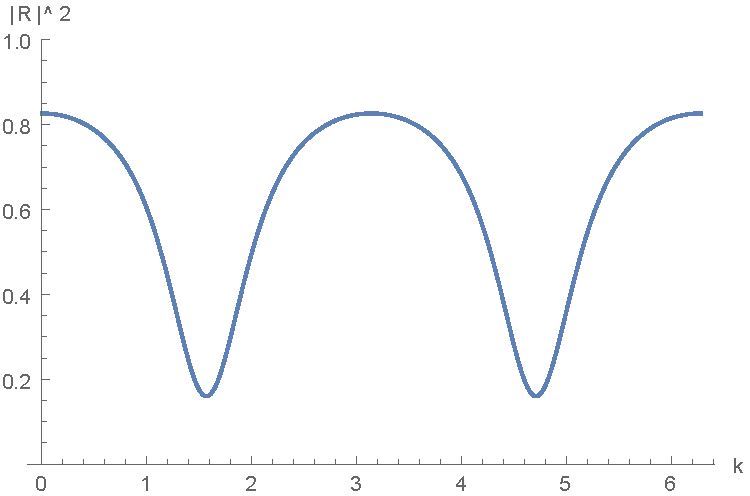
\includegraphics[width=1\textwidth]{img/2gen_reflection_l=1_b1=3_b2=7}
    \caption{$b_1=7, b_2=3$}
  \end{subfigure}
  \begin{subfigure}[t]{0.5\textwidth}
    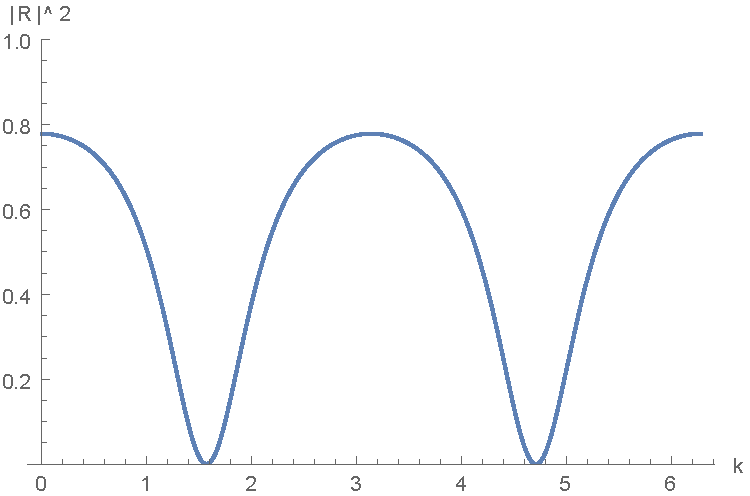
\includegraphics[width=1\textwidth]{img/2gen_reflection_l=1_b1=b2=4}
    \caption{$b_1=b_2=4$}
  \end{subfigure}
  \\
  \begin{subfigure}[t]{0.5\textwidth}
    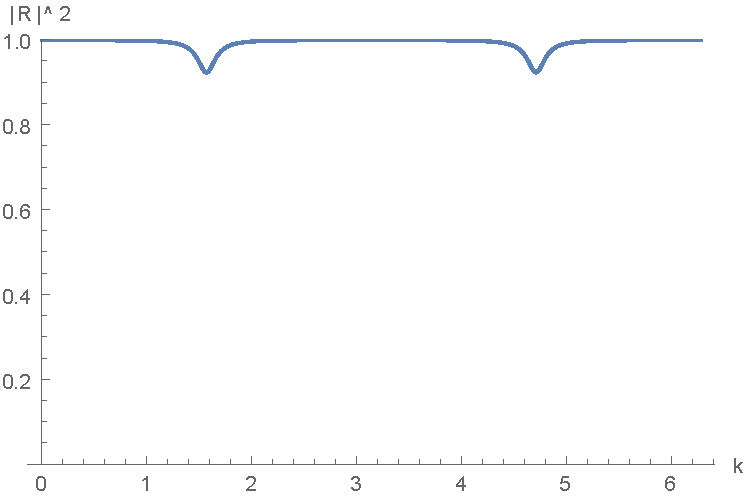
\includegraphics[width=1\textwidth]{img/2gen_reflection_l=1_b1=500_b2=10}
    \caption{$b_1=500, b_2=10$}
  \end{subfigure}
  \begin{subfigure}[t]{0.5\textwidth}
    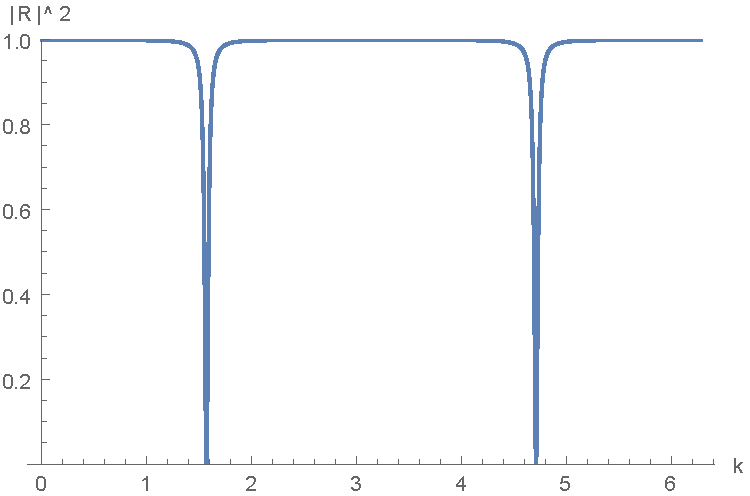
\includegraphics[width=1\textwidth]{img/2gen_reflection_l=1_b1=100_b2=100}
    \caption{$b_1=b_2=100$}
    \label{fig: 2 gen reflection gap}
  \end{subfigure}
  \caption{Reflection $\abs{R}^2$ from 2 generation radial quantum tree graph with inner edge length $\ell_1=1$ and varying branching numbers $b_1$ and $b_2$.}
  \label{fig: 2 gen reflection}
\end{figure}

Let us now consider what happens in the limiting case when one branching number grows large. As we have seen, $b_1$ and $b_2$ occurs symmetrically in the expression for $\abs{R}^2$. Hence we can without loss of generality keep $b_1$ fixed and let $b_2 \to \infty$, then from \eqref{eq: 2 gen reflection probability minimum} we see that the minimal reflection approaces 1, and thus $\abs{R} \to 1$ for all $k$. Similar to the case of the one generation radial quantum tree graph, we have the somewhat counterintuitive result that the probability of getting a reflection increases when the wave has more edges to propagate through. Keep in mind, though, that for $b_1 = b_2$ we always get zero reflection at the points $k = (2n+1)\pi/\ell_1, n = 1,2,3,\ldots$, but the interval for low reflection around these points gets smaller with increasing branching numbers, cf.\ figure~\ref{fig: 2 gen reflection gap}.

To continue this process for an arbitrary number $n$ of generations is unwieldy because one needs to calculate the determinant of a $2n \times 2n$ matrix. Instead, we will in the following chapter develop another method which makes the problem more tractable, and furthermore also gives a better insight into the scattering inside the graph.



% \section{Reflection from radial graphs with $n$ generations}

% General solutions to $Lu=u$ are
% \begin{equation}
%   \psi_j(x) = T_je^{ikx}+R_je^{-ikx}
% \end{equation}
% where $0\leq j\leq n$ is the generation number and $T_0=1, R_n=0$. The standard matching conditions give the system of equations
% \begin{equation}
%   \begin{dcases}
%     \psi_{j-1}(t_j) = \psi_j(t_j) \\
%     -\frac{d}{dx}\psi_{j-1}(t_j) + b_j\frac{d}{dx}\psi_j(t_j) = 0
%   \end{dcases}
%   \quad 1\leq j\leq n
% \end{equation}
% That is
% \begin{equation}
%   \begin{aligned}
%     % j=1: & \begin{cases}
%     %   e^{ikt_j} + R_{j-1} e^{-ikt_j} = T_j e^{ikt_j} + R_j e^{-ikt_j} \\
%     %   -ik(e^{ikt_j} - R_{j-1} e^{-ikt_j}) + b_j ik (T_j e^{ikt_j} - R_j e^{-ikt_j}) = 0
%     % \end{cases}\\
%     % 2\leq j\leq n-1: &
%     \begin{cases}
%       T_{j-1} e^{ikt_j} + R_{j-1} e^{-ikt_j} = T_j e^{ikt_j} + R_j e^{-ikt_j} \\
%       -ik(T_{j-1} e^{ikt_j} - R_{j-1} e^{-ikt_j}) + b_j ik (T_j e^{ikt_j} - R_j e^{-ikt_j}) = 0
%     \end{cases} \\
%     % j=n: & \begin{cases}
%     %   T_{j-1} e^{ikt_j} + R_{j-1} e^{-ikt_j} = T_j e^{ikt_j} \\
%     %   -ik(T_{j-1} e^{ikt_j} - R_{j-1} e^{-ikt_j}) + b_j ik T_j e^{ikt_j} = 0.
%     % \end{cases}
%   \end{aligned}
% \end{equation}
% As a matrix equation for 3 generations
% \begin{equation}
%   \begin{pmatrix}
%     -e^{-ikt_0}  & e^{ikt_0}      & e^{-ikt_0}       & 0              & 0                & 0             \\
%     ike^{-ikt_0} & b_0ike^{ikt_0} & -b_0ike^{-ikt_0} & 0              & 0                & 0             \\
%     0            & -e^{ikt_1}     & -e^{-ikt_1}      & e^{ikt_1}      & e^{-ikt_1}       & 0             \\
%     0            & -ike^{ikt_1}   & ike^{-ikt_1}     & b_1ike^{ikt_1} & -b_1ike^{-ikt_1} & 0             \\
%     0            & 0              & 0                & -e^{ikt_2}     & e^{ikt_2}        & e^{-ikt_2}    \\
%     0            & 0              & 0                & -e^{ikt_2}     & -b_2e^{ikt_2}    & b_2e^{-ikt_2} \\
%   \end{pmatrix}
%   \begin{pmatrix}
%     R \\ A \\ B \\ T_2 \\ R_2 \\ T
%   \end{pmatrix}
%   =
%   \begin{pmatrix}
%     e^{ikt_0} \\ ike^{ikt_0} \\ 0 \\ 0 \\ 0 \\ 0
%   \end{pmatrix}.
% \end{equation}


% Some observations

% \begin{itemize}
%   \item For 3 generations with equal edge lengths $\ell$ and equal branching numbers $m$ we get zero reflection iff
%   \begin{equation}
%     \cos 2k\ell = -\frac{1+m^2}{(1+m)^2}
%   \end{equation}
%   \item For any number of generations with equal length and branching number it appears to always be possible to get zero reflection.
%   \item With $m=2$ and 3 generations, zero reflection is given by at least $\ell_1=2\ell_2$ and $\ell_1=7\ell_2$, and symmetric between $\ell_1$ and $\ell_2$.
%   \item For 3 generations with equal branching number, $|R|^2$ is symmetric between the lengths.
% \end{itemize}


% \section{Minimal average reflection}


\clearpage

\chapter{The snowflake graph}\label{sec: snowflake}
\documentclass[a4paper,11pt]{report}

\usepackage[utf8]{inputenc}
\usepackage[T1]{fontenc}
\usepackage[hidelinks]{hyperref}
\usepackage[nottoc]{tocbibind}
\usepackage{caption}
\usepackage[labelformat=simple]{subcaption}
\renewcommand\thesubfigure{(\alph{subfigure})}

\usepackage{titlesec}

\usepackage{fancyhdr}


% Make section text look nice in header.
% (Only needed for article, not report.)
\makeatletter
\newcommand{\rightorleftmark}{%
  \begingroup\protected@edef\x{\rightmark}%
  \ifx\x\@empty
    \endgroup\leftmark
  \else
    \endgroup\rightmark
  \fi}
\makeatother

% hline in the footer, just like header.
\renewcommand{\footrulewidth}{0.4pt}

\pagestyle{fancy}
\renewcommand{\sectionmark}[1]{\markboth{\thesection~~~{#1}}{}}
\fancyhf{}
\lhead{\textsl{\rightorleftmark}}
\rhead{\thepage}
\lfoot{\textsc{Quantum Snowflake}}
\rfoot{\textsl{Viktor Qvarfordt}}
% \fancypagestyle{plain}{%
%   \fancyhf{}%
%   \renewcommand{\headrulewidth}{0pt}%
% }

\usepackage{mathtools,amssymb,amsthm,enumerate,cleveref}

\usepackage{tikz,tikzscale}
\usetikzlibrary{calc}

% Set up thm, def, etc.
\theoremstyle{plain}
\newtheorem{theorem}{Theorem}[chapter]
\newtheorem{proposition}[theorem]{Proposition}
\newtheorem{lemma}[theorem]{Lemma}
\newtheorem{corollary}[theorem]{Corollary}

\theoremstyle{definition}
\newtheorem{definition}{Definition}[chapter]
% \declaretheorem[name=Example,]{Ex}
\newtheorem{example}{Example}[chapter]
\AtEndEnvironment{example}{\hspace*{0pt}\hfill\ensuremath{\diamondsuit}}

\theoremstyle{remark}
\newtheorem{remark}{Remark}[chapter]

\numberwithin{equation}{chapter}

% \usepackage{showlabels}

\newcommand{\exclude}[1]{}

%% custom commands
\newcommand{\Dom}{\operatorname{Dom}}
\newcommand{\Ran}{\operatorname{Ran}}
\newcommand{\Ker}{\operatorname{Ker}}
\newcommand{\Tr}{\operatorname{Tr}}
\newcommand{\norm}[1]{\left\lVert#1\right\rVert}
\newcommand{\Norm}[1]{\lVert#1\rVert}
\newcommand{\abs}[1]{\left\lvert#1\right\rvert}
\newcommand{\ip}[2]{\ensuremath{\langle #1, #2 \rangle}}

\newcommand{\Z}{\mathbb{Z}}
\newcommand{\R}{\mathbb{R}}
\newcommand{\C}{\mathbb{C}}
\renewcommand{\H}{\mathcal{H}}

\newcommand{\D}[2]{\frac{d#1}{d#2}}
\newcommand{\pD}[2]{\frac{\partial#1}{\partial#2}}

\newcommand{\Dn}[3]{\frac{d^#3#1}{d#2^#3}}
\newcommand{\pDn}[3]{\frac{\partial^#3#1}{\partial#2^#3}}

\newcommand{\Dop}[1]{\frac{d}{d#1}}
\newcommand{\pDop}[1]{\frac{\partial}{\partial#1}}

\newcommand{\Dopn}[2]{\frac{d^#2}{d#1^#2}}
\newcommand{\pDopn}[2]{\frac{\partial^#2}{\partial#1^#2}}


\newcommand{\g}[1]{\left(#1\right)}


\title{Quantum Snowflake}
\author{Viktor Qvarfordt}


\begin{document}

\begin{titlepage}
  \thispagestyle{empty}
  % \null\vskip{-2em}
  % \noindent \large{\textbf{Stockholm University \hfill Fysikum}}
  % \vskip 7em
  \centering
  \null
  \vspace{3cm}
  {\huge\bf Quantum Snowflake} \\
  \vspace{1cm}
  {\Large\sl Viktor Qvarfordt} \\
  \vspace{0.5cm}
  {\Large May 2015} \\
  \vspace{4cm}
  {\Large Bachelor’s Thesis --- 15 ECTS} \\
  \vspace{0.5cm}
  \Large
  Supervisor: Pavel Kurasov \\
  \vspace{5cm}
  Department of Mathematics, Department of Physics \\
  \vspace{0.5cm}
  Stockholm University \\
  \vfill
  {\tiny Revised \today}
  \vspace{-1cm}
\end{titlepage}

\begin{abstract}
  Quantum graphs are defined and various general properties are explored. In particular, the Schrödinger equation is solved on the quantum snowflake graph, an infinite self-similar tree, in order to determine the graph's scattering properties. I.e.\ reflection and absorption for waves of varying energies that are sent into the snowflake graph are characterized.

By using the self-similarity and symmetries of the snowflake graph, a method is developed for reducing the snowflake graph to a line graph with special matching conditions. On this line graph, the complexity is further reduced by combining vertices into one meta-vertex. This procedure greatly simplifies the study of self-similar trees and gives a better understanding of the internal scattering of the graph.

Furthermore, it is shown that the periodic snowflake graph admits band gap structure, similar to crystalline materials. A recursive expression for the scattering coefficient for the general snowflake graph with $n$ generations is found.

\end{abstract}
% \thispagestyle{empty}
\clearpage

% \renewcommand{\abstractname}{Acknowledgments}
% \begin{abstract}
%   TODO

% \end{abstract}
% \thispagestyle{empty}
% \newpage

% \begin{figure}
%   \centering
%   \includegraphics[angle=90,width=\textwidth]{img/{snowflake_4_0.35_7_4_0.5}.pdf}
% \end{figure}

\fancypagestyle{snowflake}{\lhead{\textsl{Illustration of a quantum snowflake}}}
\thispagestyle{snowflake}
\setcounter{page}{3}
\begin{figure}
  \centering
  \includegraphics[width=\textwidth]{img/{snowflake_2_0.6_13_4_0.8}.pdf}
\end{figure}

\clearpage

{
\titleformat{\chapter}[display]{\normalfont\huge\bfseries}{\chaptertitlename~\thechapter}{20pt}{\Huge}
\titlespacing*{\chapter}{0pt}{-50pt}{25pt}
\tableofcontents
\clearpage
}

\chapter{Introduction}\label{sec: physical interpretation}\label{sec: introduction}
% \section{Preliminaries}

As the name suggests, quantum graphs model quantum mechanical particles on graph-like objects, edges joined in vertices. From a physical point of view, a quantum graph can be considered to be a network of thin (approximately one-dimensional) conductive wires on which quantum mechanical phenomena occur. On the graph, an electric and/or magnetic potential may be present. The main objective is to study how quantum mechanical particles---it is natural to consider electrons---propagate through the graph. The study of quantum graphs originated in 1930s as models for free electrons in molecules, and materials such as graphene have been modeled by quantum graphs.

% Note that we are not restricted to only quantum mechanics, in the sense that any wave-like phenomena described by sine and cosine functions or complex exponentials, such as waves in a fluid, can be modeled by the eigenfunctions of $L u = \lambda u$, where $L = - \Dopn{x}{2}$ and $\lambda$ represents the energy or frequency of the wave.

% Quantum graphs are studied both for their purely mathematical properties, and also because they are models for certain physical systems. Typical examples are systems that can be approximated as thin one-dimensional networks on which quantum mechanical phenomena occur. Indeed, quantum graphs originated as models for free electrons in molecules, and materials such as graphene have been modeled by quantum graphs.

Mathematically quantum graphs are defined as metric graphs, where edges are joined at vertices, along with a differential operator acting on functions defined on the metric graph. Most commonly one studies the eigenvalue problem of the magnetic Schrödinger operator
\[
  L_{q,a} = \g{i\Dop{x}+a(x)}^2+q(x).
\]
That is, one solves the time-independent Schrödinger equation
\[
  L_{q,a} \psi = \lambda \psi
\]
for a quantum mechanical particle living on the graph, where an electric potential $q(x)$ and magnetic potential $a(x)$ is applied. A metric graph is depicted in \cref{fig: basic quantum graph}.

\begin{figure}[h]
 \centering
  \begin{tikzpicture}[vertex/.style={draw,circle,minimum size=1.3mm,inner sep=0pt,outer sep=0pt,fill=black},scale=2, line width=0.8pt]
    \coordinate (p1) at (0,0);
    \coordinate (p2) at (1,0);
    \coordinate (p3) at (2,0);
    \coordinate (p4) at (2,1);
    \coordinate (p5) at (1.5,-0.5);
    \coordinate (p6) at (3,0.5);
    \coordinate (p7) at (2.75,-0.25);
    \coordinate (p8) at (0.75,0.75);
    % \coordinate (p9) at (3.5,0.5);
    \draw (p1)--(p2)--(p3)--(p4)--(p6);
    \draw (p2)--(p4);
    \draw (p3)--(p5);
    \draw (p2)--(p5);
    \draw (p3)--(p6);
    \draw (p3)--(p7);
    \draw (p2)--(p8);
    \draw (3.25,0.5) circle (0.25);
    \node[vertex] at (p1) {};
    \node[vertex] at (p2) {};
    \node[vertex] at (p3) {};
    \node[vertex] at (p4) {};
    \node[vertex] at (p5) {};
    \node[vertex] at (p6) {};
    \node[vertex] at (p7) {};
    \node[vertex] at (p8) {};
    % \node[vertex] at (p9) {};
  \end{tikzpicture}
  \caption{A graph.}
  \label{fig: basic quantum graph}
\end{figure}


For the equation to represent a physical system with real energies $\lambda$ one requires the operator $L_{q,a}$ to be self-adjoint. In particular this puts constraints on what can happen at the vertices, we must have certain matching conditions. The standard matching condition requires the functions to be continuous at every vertex, and in addition the sum of the outgoing derivatives from a vertex must be zero. This gives that the quantum probability of the wave is preserved after propagation through a vertex.

The purpose of this chapter is to bridge the gap between the point of view of readers more familiar with either mathematics or physics. We will introduce the aspects of quantum mechanics relevant for the study of quantum graphs and translate from the language of quantum mechanics to that of quantum graphs. More advanced concepts are deferred to the subsequent sections. In \cref{sec: defining quantum graphs} we properly define quantum graphs and further discuss metric graphs, differential operators, self-adjointness and matching conditions. In \cref{sec: properties} we explore various properties of quantum graphs and give several examples. All this builds up to \cref{sec: snowflake} where we introduce the snowflake graph, the central object of this thesis.

The quantum snowflake is defined as an infinite radial quantum tree graph that is also self-similar. By radial we mean that all properties of the graph, such as edge lengths and matching conditions, depend only on the distance from the root of the tree. The graph is self-similar in the sense that if one picks a vertex and cuts off the part of the graph that contains the root vertex, the remaining infinite subgraph is structurally identical to the original graph. In particular we require the length of every edge $e$ to be given by $\ell\beta^n$ where $n$ is the number of edges between $e$ and the root vertex, for $0<\beta<1$ we get a graph with finite depth $\ell/(1-\beta)$. On the graph we shall have standard matching conditions and no potentials.

The main objective will be to study the scattering properties of the quantum snowflake. Scattering phenomena is discussed in a more general context in \cref{sec: properties} and should be thought of as describing what information one can get out of a graph by physically examining it. To ``look'' at any object, in particular one described by a quantum graph, one shoots radiation, such as electrons, towards the object and observes how it scatters from the object. That is, we will characterize reflection and absorption for waves of varying energies that are sent into the snowflake graph.

We shall study the rotational symmetry of the snowflake graph, from which it will be possible to represent all eigenfunctions on the graph as a sum of quasi rotation invariant functions. This will allow us to collapse all edges in one generation into only one edge, from which the function values on all other edges can be reconstructed. Using this together with the self-similarity of the graph we can reduce the entire snowflake graph to a line graph with special snowflake matching conditions.

On the resulting line graph we shall further reduce the complexity by combining all vertices into one meta-vertex. This will lead to a recursive expression for the scattering coefficient for the general snowflake of $n$ generations.

This reduction of the graph greatly simplifies the study of the quantum snowflake and gives a better understanding of the internal scattering. It will be shown how the total scattering emerges from reflections on each edge of the graph.

As we will see, the general structure of the scattering from the snowflake graph is highly irregular. For the special case when the graph is periodic, i.e.\ all edges are of equal length, much more can be said. We shall show that the periodic snowflake gives rise to a band gap structure, similar to that of crystalline materials. This phenomena should be understood as arising from the fact that there exist energies that are not realizable inside the graph, therefore giving total reflection.

Finally the thesis is concluded with \cref{sec: conclusion} where we discuss of the obtained results and give indications for possible improvements and further research.




% \section{Physical interpretation}

% One should keep in mind that the mathematical models and assumptions ultimately stem from observations of nature, and can in principle not be derived mathematically. Oh really? Think about the Mathematical Universe Hypothesis.



\section{The Schrödinger equation}

It is well known that the Schrödinger equation describes the motion and behavior of quantum mechanical particles. The Schrödinger equation is often stated to be the result of empirical observations and therefore not possible to derive mathematically. However, one can arrive at the Schrödinger equation by starting from classical mechanics and imposing certain correspondence rules. In this section we motivate the Schrödinger equation by assuming that matter particles possess wave-like properties. By matter particle we mean the particles of which ordinary matter consists of, more specifically one may talk about fermions, the points is to distinguish from photons which we already know possesses wave-like properties. A more elaborate derivation of the Schrödinger equation starting from electromagnetic waves can be found in \cite{SE derivaiton}. There are indeed many ways to approach quantum mechanics and the Schrödinger equation, for instance quantization of classical mechanics or Feynman's path integral formulation, cf.\ \cite{feynman quantum mechanics}.

The following is a very naive derivation of the Schrödinger equation, illustrating how the equation arises from adding a wave-like property to classical particles, inspired by that of photons.

Let us consider a classical particle with mass $m$ and momentum $p$, the total energy is then $E = T + V$ where $T = \frac{p^2}{2m}$ is the kinetic energy and $V$ is the potential energy (from, say, an electric field) which we can leave unspecified, i.e.
\begin{equation}\label{eq: total energy}
  E = \frac{p^2}{2m} + V.
\end{equation}

We now introduce de Broglie's hypothesis, namely that matter particles possess wave-like properties just like photons. For photons we have the Planck--Einstein relation
\begin{equation}\label{eq: planck-einstein relation}
  E = h\nu
\end{equation}
relating the total energy $E$ to the frequency $\nu$ of the electromagnetic wave, where $h$ is Planck's constant. Furthermore, the energy--momentum relation states that
\begin{equation}\label{eq: energy-momentum relation}
  E^2 = (pc)^2 + (mc^2)^2
\end{equation}
for any particle, where $m$ is the intrinsic rest mass of the particle. Photons have no rest mass so this reduces to $E = pc$, where the velocity $c$ is given by $\lambda \nu$, where $\lambda$ is the wavelength. Using this we can combine the relations \eqref{eq: planck-einstein relation} and \eqref{eq: energy-momentum relation} to get
\begin{equation}\label{eq: de broglie relation}
  E = h \nu = pc = p \lambda \nu \iff p = \frac{h}{\lambda}.
\end{equation}
De Broglie's insight was that the wave-like property (which we are now introducing) of matter particles also obeys this relation, namely $p = h/\lambda$. The wavelength $\lambda$ is then interpreted as the wavelength of the matter wave associated with the particle, described by its wave function $\psi$. With no additional restrictions on the wave function it would take the general form of d'Alembert waves
\[ \psi(x, t) = f(x - vt) + g(x + vt) \]
but we will for now consider the case of simple plane waves
\[ \psi(x, t) = Ae^{i(kx - \omega t)} + Be^{i(-kx - \omega t)}. \]
(Plane waves corresponds to freely propagating waves, we will see more on this in section~\ref{sec: stationary states}.)
The wave number $k$ is related to the wavelength $\lambda$ by $k = \frac{2\pi}{\lambda}$. Using the de Broglie relation \eqref{eq: de broglie relation} we then have
\begin{equation}\label{eq: k-p relation}
  k = \frac{p}{\hbar}
\end{equation}
where $\hbar = \frac{h}{2\pi}$ is the reduced Planck constant.
Differentiating $\psi$ with respect to the spatial coordinate gives
\[ \pD{\psi}{x}(x, t) = ik\psi(x, y) = i\frac{p}{\hbar} \psi(x, t), \]
hence we have the momentum operator relation
\[ p = -i\hbar\pDop{x}. \]
We only see that this holds for plane waves $\psi(x, t) = Ae^{i(kx - \omega t)} + Be^{i(-kx - \omega t)}$, but this is indeed a general result.
Now, we can write equation \eqref{eq: total energy} as
\begin{equation}\label{eq: tise}
  E \psi = -\frac{\hbar^2}{2m}\pDn{\psi}{x}{2} + V\psi.
\end{equation}
We have arrived at the time-independent Schrödinger equation, TISE.

Furthermore, if we relate $E$ to the temporal frequency $\frac{\omega}{2\pi}$ of the wave function via the Planck--Einstein relation \eqref{eq: planck-einstein relation}---which we can use since we have assumed a wave-like property matter particles similar to that of photons---we have
\[ E = \hbar \omega. \]
Differentiating $\psi$ with respect to the temporal coordinate, and using the above relation, gives
\[ \pD{\psi}{t}(x,t) = -iw\psi(x,t) = \frac{-iE}{\hbar} \psi(x,t), \]
that is
\begin{equation}
  E\psi(x,t) = i \hbar \pD{\psi}{t}(x,t).
\end{equation}
Substituting this for the left hand side in the time-independent Schrödinger equation \eqref{eq: tise} gives
\begin{equation}\label{eq: tdse}
  i \hbar \pD{\psi}{t} = -\frac{\hbar^2}{2m}\pDn{\psi}{x}{2} + V\psi,
\end{equation}
the time-dependent Schrödinger equation, TDSE.

In our example we can introduce the Hamiltonian $H$ as the operator defined by the expression
\[ H = \widehat{T} + \widehat{V} = -\frac{\hbar^2}{2m}\pDopn{x}{2} + V(x) \]
where
\[ \widehat{T} = -\frac{\hbar^2}{2m}\pDopn{x}{2} = \frac{\widehat{p}^2}{2m} \]
is identified as the kinetic energy operator with
\[ \widehat{p} = -i \hbar \pDop{x} \]
being the momentum operator and $\widehat{V} = V(x)$ is the potential energy operator. The TDSE can then be written more compactly as
\[ i\hbar \pD{\psi}{t} = H\psi \]
and the TISE becomes an eigenvalue equation for the operator $H$
\[ H\psi = E\psi. \]
The Hamiltonian recovered above is the usual Hamiltonian for a particle propagating under the influence of a potential $V(x)$, but for other particular systems the Hamiltonian may take another form.
If we use natural units where $\hbar=1$ and let the $m = 1/2$, so that $\frac{\hbar^2}{2m} = 1$, and denote the energy in these normalized units by $\lambda$, then the TISE for the usual Hamiltonian can be written as
\[ L_q\psi = \lambda\psi. \]
That is $H = L_q$ where $L_q$ was defined in \eqref{eq: magnetic schrödinger operator}. The magnetic potential is taken into account by letting
\[ \widehat{p} = -i \pDop{x} - a(x), \]
then $H = L_{q,a}$. In the subsequent sections we will only use normalized units, as described above.



\section{Quantum states and interpretations of quantum mechanics}\label{sec: quantum states and interpretations of quantum mechanics}

Classically, properties of an object, or the \emph{state} of an object, is characterized by its position and momentum. In quantum mechanics the state of a particle is instead specified by its wave function, containing information about both the position and momentum of the particle. The Schrödinger equation gives the possible such states, their corresponding energies, and how they evolve over time.

A fundamental property of quantum mechanics is that quantities such as energy for a particle can be constrained to discrete values, for example the energy of an electron bound to an atom. However, a freely propagating electron can take energies from a continuous spectrum. Recall from section~\ref{sec: spectrum} that the spectrum of linear operators may have this property, namely the spectrum can be both discrete and continuous. It is therefore a postulate of quantum mechanics that to each dynamical variable, ``observable'', there corresponds a linear operator such that all possible values of the variable are given by the spectrum of the operator.

The \emph{ground state energy} (zero-point energy) is the lowest positive eigenvalue $\lambda_0$, the higher eigenvalues are called excited state energies.

% For many graphs also $\lambda = 0$ is an eigenvalue, however this energy is not physically realizable because of the uncertainty principle. As can be shown, the wave function $\psi(x)$ in position space and wave function $\widetilde{\psi}(p)$ in momentum space are Fourier transform duals of each other. Hence we have $\sigma_x\sigma_p \le 1$, where $\sigma_a$ denotes the standard deviation of a variable $a$, (the lower bound depends on which particular definition of the Fourier transform that is being used, and what units we assume). From this we see that $E=0$ is not possible, since this is implies zero kinetic energy, i.e.\ zero momentum, hence $E>0$.

The statistical interpretation of quantum mechanics, introduced by Max Born in \cite{born statistical interpretation}, originally motivated entirely by observation, states that the probability of observing a quantum mechanical particle at a particular location $x$ and time $t$ is given by the probability density function $\abs{\psi(x,t)}^2$, this fact is known as the Born rule.
% This also exemplifies why one requires $\psi \in L^2$, so that the total probability equals unity.

Although this thesis primarily deals with the mathematical properties of quantum graphs, we will broaden our view of the physical significance of the mathematics and highlight questions that arise when interpreting the models by making a slight detour into the interpretation of quantum mechanics, by discussing the so called measurement problem.

Quantum mechanical particles are often spread out in space, in the sense that $\psi(x)$ is non-zero on some interval (in fact, time evolution tends to smear out the wave function), while on the other hand, a measurement of the position of a particle always yields a specific position, in accordance with the Born rule. The wave-like property can only be implicitly detected by studying interference of the wave function.
% In the context of quantum graphs, the stationary states of any graph have a wave function that is non-zero almost everywhere on the entire graph, while any attempt to measure the position of the particle will yield a specific position.

This seemingly collapse of the wave function, from being smeared out to becoming highly localized, is not in any way described by the mathematics of quantum mechanics. The text-book approach of describing this is by adding a postulate to the model, namely that the wave function collapses (i.e.\ becomes highly localized) to the measured value. This is what is known as the Copenhagen interpretation. This interpretation arguably has several issues, for example, what precisely constitutes a measurement? Any interaction of particles is in a sense a measurement. Einstein's objection is often quoted as ``God does not throw dice'', pointing out that the random collapse of the wave function is ill-justified and not consistent with our otherwise deterministic model of reality. Other so called collapse theories exist, perhaps most noteworthy is the Ghirardi--Rimini--Weber theory, postulating that the wave function undergoes spontaneous collapse and random yet very frequent points in time. This avoids the problem of what denotes a measurement in the Copenhagen interpretation while still giving predictions that are in agreement with observations.

Any collapse theory will necessarily contain fundamental randomness. This may seem unavoidable if the Born rule is to be satisfied, but this is not the case. The mathematically simplest interpretation is to not add any additional postulates, contrary to the other interpretations, that is to say that the wave function never collapses, it continues to evolve deterministically according to the Schrödinger equation. In this interpretation every measurement entangles the ``observer'' to the measured system, thus entering a superposition state. Measurements are then not distinguished from any other form of interaction between particles, unlike in the Copenhagen interpretation.

This entails that the entire environment gets entangled to the quantum state being measured, from which the classical state emerges as an apparent collapse of the wave function, an effect called decoherence. In this interpretation every possible classical state exists in a superposition. This gives rise to the Many Worlds Interpretation originally introduced by Hugh Everett, in which, by the effect of decoherence, non-interacting branches of the wave-function (and in extension reality) get created. The Born rule is then an emerging property in every decohered slice of reality \cite{carroll EQM probability, wallace born rule}.

One may argue that the interpretation is not important, since all interpretations give equal predictions, but this is not necessarily the case. There are contrived gedanken experiments for which, for example, collapse theories and the many world theory gives different predictions \cite{vaidman mwi}.

A radically different approach is Quantum Bayesianism, in which one assumes that quantum states do not represent elements of physical reality \cite{qbism introduction, qbism and the greeks}. This is a rather pragmatic approach in which quantum mechanics is merely a tool for making statistical predictions, in this way avoiding the problematic implications of interpreting quantum states as representations of physical reality.

Towards the other extreme we have the Mathematical Universe Hypothesis by Max Tegmark \cite{tegmark}, essentially extending from the Many worlds interpretation, postulating that the physical world is an abstract mathematical structure. Hence stating that quantum states truly are elements of physical reality (provided that quantum mechanics is a correct description of reality).

There is no consensus on how quantum mechanics is to be interpreted, and the discussion quickly becomes philosophical. There is however no doubt in that it is a very successful theory in the sense that all predictions so far are in perfect agreement with empirical results.
% In what follows we will generally not be concerned with interpretations and when necessary we will apply the Born rule without further ado.



\section{Stationary states}\label{sec: stationary states}

Stationary states are states that do not evolve over time, in the sense that $\abs{\psi(x,t)}^2$ is constant in $t$, stationary. This allows for a time dependence of the probability amplitude $\psi(x,t)$ only as a phase shift $e^{i\theta(t)}$, where $\theta(t) \in \R$. As we will see in equation \ref{eq: time-separated solution}, the phase is given by $\theta(t) = -\lambda t$. Stationary states are important since they are the states of equilibrium, states reached after some time when the system has settled.
% The study of quantum graphs mainly focuses on such states.
% General solutions to the Schrödinger equation can be expressed as a series of stationary states, therefore most attention is directed towards stationary states.
Considering only stationary states greatly simplifies matters, since the TISE is an ordinary differential equation while the TDSE is a partial differential equations. On the other hand, every solution to the TDSE can be written as a superposition of stationary states, showing that it is essentially sufficient to consider such states.

The stationary solutions to the time-dependent Schrödinger equation \eqref{eq: tdse} can be found by using separation of variables with the Ansatz
\[ \psi(x,t) = u(x) T(t). \]
This then gives, with $q(x) \equiv a(x) \equiv 0$ for convenience,
\[
  i \Dop{t} u(x) T(t) = - \Dopn{x}{2} u(x) T(t) \iff
  i \frac{\D{T}{t}(t)}{T(t)} = - \frac{\Dn{u}{x}{2}(x)}{u(x)} = \lambda,
\]
for some constant $\lambda$. That is,
\begin{align*}
  i \D{T}{t}(t) &= \lambda T(t) \\
  - \Dopn{x}{2}u(x) &= \lambda u(x).
\end{align*}
The second equation is precisely the time-independent Schrödinger equation for the spatial component $u(x)$, justifying that the constant $\lambda$ is to be interpreted as the energy of the system (in normalized units). With $k^2 = \lambda$ we can write the solutions for $u(x)$ as
\[ u(x) = Ae^{ikx} + Be^{-ikx} \]
and the solution for the time component $T(t)$ as
\begin{equation}\label{eq: time-separated solution}
  T(t) = e^{-i\lambda t}.
\end{equation}
Hence the solution to the TDSE is given by
\begin{equation}\label{eq: left right waves}
  \psi(x,t) = Ae^{i(kx-\lambda t)} + Be^{i(-kx-\lambda t)},
\end{equation}
showing that the two terms can be interpreted as right and left traveling waves, respectively. The constants $A$ and $B$ and possible values of $\lambda$ are to be determined by the particular situation, see for instance example~\ref{ex: particle in a box}.

The wave function of a stationary state is given by standing waves, evolving in time only by changing the phase shift.

The criteria of $H$ being self-adjoint, discussed in \ref{sec: differential operators}, is important in the quantum mechanical interpretation. It ensure that the model is physical in the sense that the eigenvalues of $H$ are real, which is necessary since this represents the energy of the system. Furthermore, the eigenvectors of $H$ are then orthogonal and can be chosen so that they form an orthonormal basis of the state space. This, together with the linearity of the equation, allows any solution of the TDSE to be written as a linear combination of stationary states, showing that it is sufficient, without loss of generality, to consider only the stationary states.



\clearpage

\fancypagestyle{automatic}{\lhead{\textsl{\rightorleftmark}}}
\pagestyle{automatic}

\chapter{Defining quantum graphs}\label{sec: defining quantum graphs}
This section is devoted to defining and discussing quantum graphs and the components that it consists of. A more thorough introduction and characterization of quantum graphs can be found in the survey article \cite{introduction and brief survey} or the books \cite{pavel book} and \cite{berkolaiko kuchment book}. We begin by defining exactly what is meant by a quantum graph. The meaning of the terms will be explained in the following sections.

\begin{definition}
  A \emph{quantum graph} is a triple $(\Gamma, L, \text{MC})$, where
  \begin{itemize}
    \item $\Gamma$ is a \emph{metric graph},
    \item $L$ is a \emph{differential expression} defined on a function space on $\Gamma$, and
    \item MC is a set of equations, \emph{matching conditions}, relating the limit values  of the functions defined on the edges of $\Gamma$.
  \end{itemize}
\end{definition}

Similar to how, in abstract algebra, one talks about a group $(G,*)$ by referring to its underlying set $G$, we will often talk about a given quantum graph $(\Gamma, L, \text{MC})$ by referring to the metric graph $\Gamma$, often called the \emph{underlying (metric) graph}.

Initially the quantum graph is only given a differential expression $L$. Next, one defines a corresponding differential operator whose action is given by the differential expression, furthermore one must determine the domain of the operator, so that the operator satisfies desired properties such as being self-adjoint. The domain of the operator is not known \textit{a priori}, therefore we only include a differential expression in the definition of a quantum graph.
% Usually one chooses $L$ so that the eigenvalue problem $L\psi=\lambda\psi$ is the Schrödinger equation, or some other equation of interest.
The three components in the definition are dependent of each other in the sense that one often defines the underlying metric graph from the geometry of the problem. The differential operator is then defined as acting on functions defined on the edges of this graph, satisfying the matching conditions to ensure self-adjointness and other properties of interest.

As we will see in \cref{sec: snowflake}, two graphs of different geometry, i.e.\ having different underlying metric graphs, can be equivalent by a certain choice of matching conditions for the ``geometrically altered'' graph. This turns out to be a powerful method of simplifying studies of more complicated graphs.

It is natural to begin our discussion with metric graphs, which we now proceed to define.



\section{Metric graphs}\label{sec: metric graphs}

In discrete mathematics, combinatorial graphs are defined as vertices connected to each other through edges. The edges merely reflect the relation between vertices, which are the main objects of the graph. Metric graphs can then be defined as combinatorial graphs with weights assigned to each vertex, but it is useful to change the point of view slightly.

In contrast to combinatorial graphs, the main objects of metric graphs are the edges, while the vertices merely reflect the relation between edges. Let us now formally define a metric graph, note how we still have vertices and edges, but they play a very different role.

\begin{definition}
  A \emph{metric graph} is a tuple $(E,V)$ where
  \begin{itemize}
    \item $E = \{e_n\}_{n=1}^N$ is a set of intervals $[x_{2n-1}, x_{2n}] \subset \R$ called \emph{edges}, where $x_{2n-1} < x_{2n}$. At least one end-point of each interval must be finite. If both end-points are finite then the edge is called compact, otherwise it is called semi-infinite.
    \item $V = \{v_m\}_{m=1}^M$ is a partition of the set of all end-points of edges in $E$, each element in $V$ is called a \emph{vertex}. End-points belonging to the same vertex (partition) are identified as the same point.
  \end{itemize}
\end{definition}

It is this construction of the vertices that defines the connection between the otherwise completely independent edges in $E$. The partition of endpoints into vertices, or the equivalence relation giving rise to it, can thus be viewed as defining the geometry of the graph, or vice versa.

It is useful to think of metric graphs as intervals of the real line, being the edges, joined together at some of their end-points, being the vertices. The physical interpretation could then be thin metal wires welded together at some points, we will come back to this after we have introduced the differential operator acting on the graph.

Similar to combinatorial graphs, we define the \emph{degree} $\deg v_m$ of a vertex $v_m$ to be the number of edges connected through this vertex. Equivalently it is the number of edges containing the vertex, i.e.\ the degree is simply $\abs{v_m}$, the number of end-points belonging to the vertex.

A metric graph $\Gamma$ is said to be connected if there exists a continuous path in $\Gamma$ connecting $x$ and $y$ for every $x, y \in \Gamma$. If this does not hold for every $x$ and $y$ the graph is considered to be split into a number of disconnected subgraphs or connected components, each being a connected graph containing at least one edge. If a graph has several connected components, they can be considered to be completely independent graphs, in this text we shall only be interested in connected graphs.

Unlike combinatorial graphs, edges $e_n$ in metric graphs have the notion of length, simply defined as $\ell_n = x_{2n} - x_{2n-1}$. From this we can define the total length of a graph as $\mathcal{L} = \sum_{n=1}^{N} l_n$. We also introduce a distance $d(x, y)$ between any two points $x$ and $y$ in a connected metric graph as the length of the shortest path between $x$ and $y$.

We now define what is meant by a function being defined on the graph, we often consider functions from the following functions spaces.

\begin{definition}[Function spaces on metric graphs]
  Let $\Gamma$ be a metric graph, the Hilbert space $L_2(\Gamma)$ is then the direct sum of the $L_2$ spaces on each edge of $\Gamma$. That is the set of all functions that are square integrable on each edge:
  \[
    L_2(\Gamma) = \bigoplus_{e \in E} L_2(e).
  \]
  Similarly we define the Sobolev space $W_2^2(\Gamma\setminus V)$ as the set of all square integrable functions with weak derivatives up to order 2 being square integrable:
  \[
    W_2^2(\Gamma\setminus V) = \bigoplus_{e \in E} W_2^2(e).
  \]
  Analogously we define $C^\infty_0(\Gamma\setminus V)$ as the set of smooth functions with support separated from the vertices of $\Gamma$.
\end{definition}

We will also need the notion of inner product between two functions on the graph.

\begin{definition}[$L_2$ inner product and norm on metric graphs]\label{def: inner product on graph}
  The $L_2$ inner product on a metric graph $\Gamma$ is given by
  \[
    \ip{f}{g}_{L_2(\Gamma)} =
    \sum_{e \in E} \ip{f}{g}_{L_2(e)} =
    \sum_{e \in E} \int_e f(x)\overline{g}(x)\,dx
  \]
  which we can write as $\int_\Gamma f(x)\overline{g}(x)\,dx$, where $\overline{z}$ denotes complex conjugation of $z$.
  The $L_2(\Gamma)$ norm is then naturally defined by
  \[
    \norm{f}_{L_2(\Gamma)} = \ip{f}{f}_{L_2(\Gamma)} = \int_{\Gamma} \abs{f(x)}^2 dx.
  \]
\end{definition}

These definitions are very natural generalizations of the same concepts on intervals of $\R$, further adding to the notion that metric graphs are merely sets of intervals of $\R$ that share some end-points.

A function $f$ defined on $\Gamma$ is simply a function defined independently on each edge. This leads to the problem of $f(x_j)$ not being well defined where $x_j \in v$ for some vertex $v$. Points in $v$ are by definition identified as the same point but the definition of $f$ does not reflect this. If $f$ is continuous on each edge we can define $f(x_j)$ as
\begin{align*}
  f(x_{2n}) &= \lim_{x \to x_{2n}^-} f(x) \\
  f(x_{2n-1}) &= \lim_{x \to x_{2n-1}^+} f(x),
\end{align*}
that is, the limits are taken as one-sided limits from the inside of the edge. Later we will consider functions continuous on the entire graph, in which case even $f(v)$ will be well defined.

As we've seen it is natural to consider limits at a vertex as the one-sided limit taken from inside the edge. Motivated by this we introduce the following.

\begin{definition}
  The \emph{normal derivative} $\partial f(x_j)$ of a function $f$ on a metric graph $\Gamma$ at an end-point $x_j$ of an edge is given by
  \begin{align}
    \partial f(x_j) =
    \begin{dcases}
      \lim_{x \to x_j}   \Dop{x} f(x) & j = 2n-1 \\
      \lim_{x \to x_j} - \Dop{x} f(x) & j = 2n
    \end{dcases}
  \end{align}
\end{definition}

This should be understood as taking the derivative in the direction into the edge, out from the vertex given by the end-point $x_j$. This is a useful concept since it allows us to disregard the direction of parametrization of the edge. For this graph it is indeed only the length of an edge that is of relevance, in section~\ref{sec: edge parametrization} we will consider how edge parametrization affects graphs in general.



\section{Differential operators}\label{sec: differential operators}

We now introduce the differential operator acting on function from the function space of the underlying metric graph. The differential operator can be seen as defining which phenomena is being studied on the graph. The most simple and common operator is the \emph{Laplace operator}
\begin{equation}\label{eq: laplacian}
  L = - \Dopn{x}{2}.
\end{equation}
Note that the domain of the operator must be carefully defined, as we shall see in section~\ref{sec: self-adjoint operators}, the domain plays a very important role for properties of the operator, such as self-adjointness. Until then, let us consider the simple case $\Dom L = C^2(\R)$, in order to get a preliminary understanding of the operators that will come into play. The eigenfunctions $u(x)$ of $L$, satisfying
\[ Lu = \lambda u, \] are complex waves which can be written as
\[ u(x) = Ae^{ikx} + Be^{-ikx}, \quad k^2 = \lambda. \]
Solving the eigenvalue problem $Lu=\lambda u$ amounts to studying wave propagation through one-dimensional structures connected at the vertices, being the graph $\Gamma$. In order to do this properly we must define matching conditions at the vertices, as we shall do in section~\ref{sec: mc}.

Because of the relation
\[
  Ae^{ikx} + Be^{-ikx} = C\cos kx + D\sin kx
\]
for complex constants $A, B, C$ and $D$ such that $C=A+B$ and $D=i(A-B)$, we can chose to represent the eigenfunctions of $L$ as complex exponentials or trigonometric functions. We will see that in different contexts one representation may be more convenient than the other. If one wants to emphasize the evenness or oddness of the eigenfunction, c.f.~\ref{ex: even odd eigenfunctions}, the trigonometric representation is superior. On the other hand the complex exponential form splits the eigenfunction into left and right traveling waves, c.f.~\ref{eq: left right waves}.

More generally one introduces the \emph{Magnetic Schrödinger operator}
\begin{equation}\label{eq: magnetic schrödinger operator}
  L_{q,a} = \left(i\Dop{x} + a(x)\right)^2 + q(x)
\end{equation}
where $a(x)$ is the magnetic potential and $q(x)$ is the electric potential present on the graph. With no magnetic potential we denote $L_{q,0} = L_q$ simply as the \emph{Schrödinger operator}. Note also that $L_{0,0} = L$. The eigenfunctions of $L_{q,a}$ describe the stationary states of quantum mechanical particles on the graph under the influence of electric and magnetic potential. In particular, $L_q \psi = \lambda \psi$ is the standard time-independent Schrödinger equation, see \cref{sec: physical interpretation} for more details on the physical interpretation.

Before we proceed we shall formalize the notion of operators and consider some of their properties.
% We outline only the basics and important notions that will later be used. More information can be found in any book on functional analysis.


\subsection{Operator formalism}

Let us first recall that an operator $A$ is a mapping between two linear vector spaces $X$ and $Y$ with scalars in $\C$,
\[ A : X \to Y. \]
The operator is said to be linear if $A(\alpha x + \beta y) = \alpha A x + \beta A y$ where $x,y \in X$ and $\alpha, \beta \in \C$.
We shall mostly be concerned with the case when $X$ and $Y$ are function spaces, such as the introduced Sobolev space $W_2^2(\Gamma\setminus V)$. In this case we write $(Af)(x)$, i.e. $A$ operates on a function $f \in X$ and gives a function $Af \in Y$, which in turn is applied to an element $x$ from the domain of functions in $Y$.
Composition $(ABf)(x)$ of two operators $A$ and $B$ is to be understood as $A(B(f(x)))$.
The following example shows how to work with operator expressions and that, in general, operators do not commutative.

\begin{example}
  Let $A$ and $B$ be two operators defined on the same function space, the equation
  \[ A = B \]
  should be understood as
  \begin{enumerate}[i)]
    \item $\Dom A = \Dom B$
    \item $Af = Bf$ for every function $f$ in the domain.
  \end{enumerate}
  The importance of this is exemplified by considering the operators
  \[ A = \Dop{x}, \quad B = g(x), \]
  where $A$ is the derivative operator and $B$ is simply pointwise multiplication by a continuously differentiable function $g(x)$. Let the domain of both operators be $C^1(\R)$. It is not true that
  \begin{equation*}
    AB = \frac{d}{dx}g(x) = g'(x),
  \end{equation*}
  which is clear if we let $AB$ act on a function
  \begin{align*}
    (ABf)(x) &= \big(A(Bf)\big)(x) \\
    &= \frac{d}{dx}\Big(g(x)f(x)\Big) \\
    &= g'(x)f(x)+g(x)f'(x) \\
    &= \left(g'(x)+g(x)\Dop{x}\right)f(x).
  \end{align*}
  That is,
  \[ AB = g'(x)+g(x)\frac{d}{dx}, \]
  which shows that caution must be exercised when dealing with operator expressions.
  On the other hand we have
  \[ (BAf)(x) = g(x)f'(x), \]
  showing that
  \[
    BA = g(x)\Dop{x}
  \]
  In conclusion we have that the commutator between $A$ and $B$ is given by
  \[
    AB-BA = g'(x).
  \]
\end{example}

We now state some important definitions.

\begin{definition}[Bounded operator]
  An operator $A: X \to Y$ is said to be \emph{bounded} if there exists a constant $C$ such that
  \[
    \norm{Ax} \le C \norm{x} \quad \forall x\in X.
  \]
  Furthermore, the infimum over all such constants $C$ is called the \emph{norm} of $A$, denoted by $\norm{A}$. If no such $C$ exists, we say that $A$ is unbounded.
\end{definition}

\begin{definition}[Isometric operator]
  An operator $A: X \to Y$ is said to be \emph{isometric (norm preserving)} if
  \[ \norm{Ax}_Y = \norm{x}_X \quad \forall x \in X. \]
\end{definition}

\begin{definition}[Unitary operator]
  An operator $A: X \to Y$ is said to be \emph{unitary} if it is defined on the whole space $X$, is isometric and surjective. In particular this gives that $A$ is invertible and
  \[ AA^* = A^*A = I. \]
\end{definition}

To properly define an operator $L: X \to Y$, its domain $\Dom(L) \subseteq Y$ must be specified. As it turns out, the domain of an operator plays a very important role for the properties of the operator.

\begin{example}[Shift operator]
  Consider the space $\ell^2$ consisting of all infinite sequences $\vec{x}=(x_1, x_2, \ldots)$ with
  \[
    \norm{\vec{x}}_2 = \sqrt{\sum_{n=1}^{\infty} \abs{x_n}^2} < \infty.
  \]
  Define the \emph{shift operator} $S$ on $\ell^2$ by
  \[
    S(x_1, x_2, \ldots) = (0, x_1, x_2, \ldots).
  \]
  Clearly $S$ is an isometry, the norm of $\vec{x}$ is preserved for every $\vec{x} \in \ell^2$:
  \[
    \norm{S(\vec{x})}
    = \norm{(0,x_1,x_2,\ldots)}
    = \sqrt{\sum_{n=1}^{\infty} \abs{x_n}^2 }
    = \norm{(x_1, x_2, \ldots)}
    = \norm{\vec{x}}.
  \]
  However, $\Ran S \ne \ell^2$ since any element $\vec{x} = (x_1, x_2, \ldots)$ with $x_1 \ne 0$ is not contained in $\Ran S$. Hence, the shift operator $S$ is not surjective and thus not unitary.
\end{example}




\subsection{Self-adjoint, symmetric and hermitian operators}\label{sec: self-adjoint operators}

\begin{quote}\itshape
  ``In the 1960s Friedrichs met Heisenberg, and used the occasion to express to him the deep gratitude of the community of mathematicians for having created quantum mechanics, which gave birth to the beautiful theory of operators in Hilbert space. Heisenberg allowed that this was so; Friedrichs then added that the mathematicians have, in some measure, returned the favor. Heisenberg looked noncommittal, so Friedrichs pointed out that it was a mathematician, von Neumann, who clarified the difference between a self-adjoint operator and one that is merely symmetric. `What's the difference', said Heisenberg.'' \normalfont\cite[p.~414]{lax}
\end{quote}

As the quote above indicates, there is often confusion regarding the concepts of self-adjoint, symmetric and hermitian operators. The topic of functional analysis, operator theory and in particular unbounded self-adjoint operators is deep, and we shall only touch upon the topics directly related to the study of quantum graphs, further details can be found in \cite{teschl-fa, teschl-schroe, schmudgen}. What is presented below is mainly taken from \cite[section 1.2]{schmudgen} and \cite[section 5.1]{pedersen}. Recall first that a Hilbert space is a complete inner-product space.
% The difficulty arises when the operator is unbounded, which also is the most interesting case since the operators $L_{q,a}$ we are working with are unbounded operators.

Let $\H_1$ and $\H_2$ be Hilbert spaces and let $T$ be a linear operator from $\H_1$ to $\H_2$ such that the domain $\Dom T$ is a linear subspace that is dense in $\H_1$, that is $\overline{\Dom T} = \H_1$ where $\overline{\Dom T}$ denotes the closure of $\Dom T$. Set
\[
  \Dom T^* = \{y \in \H_1 \mid \text{the functional } x \mapsto \ip{Tx}{y}_2 \text{ on } \Dom T \text{ is bounded} \}.
\]
Since $\Dom T$ is dense in $\H_1$, the functional $x \mapsto \ip{Tx}{y}_2$ extends by continuity to $\H_1$ (a linear functional is bounded if and only if it is continuous \cite[theorem 4.4.2]{friedman}). By Riesz's theorem \cite[theorem 6.2.4]{friedman} there exists a unique element $z \in \H_1$ such that $\ip{Tx}{y}_2 = \ip{x}{z}_1$. Hence we can set $T^*y = z$ to obtain a well-defined mapping $T^*$ from $\H_1$ to $\H_2$, and we have
\begin{equation}\label{eq: adjoint symmetric relation}
  \ip{Tx}{y}_2 = \ip{x}{T^*y}_1 \quad \forall x \in \Dom T, \; y \in \Dom T^*.
\end{equation}

\begin{definition}[Adjoint operator]
  Let $T$ be a densely defined linear operator from $\H_1$ to $\H_2$, both being Hilbert spaces.
  The operator $T^*$ as described above is called the \emph{adjoint} operator of $T$.
\end{definition}

If $S$ and $T$ are two linear operators from $\H_1$ to $\H_2$ we say that $S = T$ if and only if their domains coincide, i.e.\ $\Dom S = \Dom T$, and additionally $S(x) = T(x)$ for all $x$ in the domain. If $\Dom S \subseteq \Dom T$, and if the operators agree on the common domain, that is $S(x) = T(X)$ for all $x \in \Dom S$, then we say that $S$ is a restriction of $T$ or equivalently that $T$ is an extension of $T$, and write $S \subseteq T$.

\begin{definition}[Symmetric operator]
  Let $T$ be a densely defined linear operator on a Hilbert space, then $T$ is called \emph{symmetric} if $T \subseteq T^*$.
\end{definition}

\begin{definition}[Self-adjoint operator]
  Let $T$ be a densely defined linear operator on a Hilbert space, then $T$ is called \emph{self-adjoint} if $T = T^*$.
\end{definition}

% \begin{definition}[Symmetric operator]
%   An operator $T$ defined on a Hilbert $\H$ space is called symmetric if
%   \[
%     \ip{Tx}{y} = \ip{x}{Ty} \quad \text{ for all } x, y \in \Dom(T) \subseteq \H.
%   \]
% \end{definition}

% \begin{definition}[Adjoint]
%   Let $T$ and $T^*$ be operators on a Hilbert space $\H$ space such that
%   \begin{equation*}
%     \ip{Tx}{y} = \ip{x}{T^*y} \quad \text{ for all } x, y \in \H,
%   \end{equation*}
%   then $T^*$ is called the \emph{adjoint} of $T$. If $T$ is everywhere defined and in particular $T=T^*$ we say that $T$ is self-adjoint.
% \end{definition}


The definition of Hermitian operators is not as well standardized, often it is used interchangeably with symmetric or self-adjoint operators. Sometimes it is only used for finite-dimensional spaces where the matrix representation of the adjoint of an operator $A$ equals the hermitian conjugate of the matrix representation of $A$.

Some important properties of self-adjoint operators are that the eigenvalues are always real \cite[p.~16]{ballentine} and eigenvectors corresponding to distinct distinct eigenvalues can always be chosen to be orthogonal \cite[p.~17]{ballentine}.

Note that in the above definitions, the condition that $\Dom T$ is dense in $\H$ along with the uniqueness of Riesz's theorem is necessary to conclude that the adjoint operator $T^*$ of $T$ is unique.
% Indeed, if $\overline{\Dom T} \ne \H$ then $\ip{Tx,y} = \ip{x,T^*y} = \ip{x,T^*y+w}$, where $w$ is any element orthogonal to

\exclude{
The following example illustrates the relation between symmetric and self-adjoint operators.

\begin{example}\label{ex: self-adjoint example 1}
  Let $L = -\Dopn{x}{2}$ and let the domain of $L$ be
  \[
    \Dom L = \{u \in L_2([0, \infty)): u(0) = u'(0) = 0 \}.
  \]
  We now verify that $L$ is symmetric by partial integration:
  \begin{align*}
    \ip{Lu}{v}
    &= \int_{0}^{\infty} (Lu)(x)\overline{v(x)} dx \\
    &= \int_{0}^{\infty} (-u''(x))\overline{v(x)} dx \\
    &= \int_{0}^{\infty} u'(x)\overline{v'(x)} dx - \left[u'(x)\overline{v(x)}\right]_{0}^{\infty} \\
    &= \int_{0}^{\infty} u(x)(-\overline{v''(x)}) dx + \left[u(x)\overline{v'(x)} - u'(x)\overline{v(x)}\right]_{0}^{\infty}.
  \end{align*}
  Note that the final integral is precisely $\ip{u}{Lu}$ and since the functions are square integrable they must vanish for $x\to\infty$, thus we get
  \[
    \ip{Lu}{v} = \ip{u}{Lv} - u(0)\overline{v'(0)} + u'(0)\overline{v(0)}.
  \]
  The boundary terms $-u(0)\overline{v'(0)} + u'(0)\overline{v(0)}$ vanish by the assumption on $\Dom L$, namely that the functions $u$ satisfy $u(0) = u'(0) = 0$.
  The domain of $L^*$ is the set of all $v \in L_2$ for which $L^*$ is a bounded linear functional. Since we have $u(0)=u'(0)=0$, we must have $v(0)=v'(0)=0$ for otherwise $L^*$ would be unbounded since

  This is given by the set of all $v \in L_2$ for which the boundary terms vanish, so that
  \[
    \ip{Lu,v} = {u,L^*v} \quad \forall x \in \Dom T, \; y \in \Dom T^*,
  \]
  c.f.\ equation \eqref{eq: adjoint symmetric relation}. As we see from the above calculation, we do not need to put any additional constraints on the functions $v$, the boundary terms vanish by definition of $\Dom L$. Hence we have $\Dom L \subset \Dom L^*$, that is $L \subset L^*$ showing that $L$ is symmetric but not self-adjoint.
\end{example}

\begin{example}
  Consider again $L = -\Dopn{x}{2}$ but with the domain of $L$ given by
  \[
    \Dom L = \{u \in L_2([0, \infty)) : u'(0) = h u(0) \},
  \]
  for fixed $h\in\C$.
  By similar calculations as in example~\ref{ex: self-adjoint example 1} we have
  \begin{align*}
    \ip{Lu}{v} = \int_{0}^{\infty} u(x)(-\overline{v''(x)} dx + u(0)\overline{v'(0)} - u'(0)\overline{v(0)}
  \end{align*}
  where the boundary terms can be written as
  \begin{align*}
    u(0)\overline{v'(0)} - u'(0)\overline{v(0)} = u(0) \g{\overline{v'(0)}-h\overline{v(0)}}.
  \end{align*}
  The boundary terms vanish for all $u$ and $v$ if and only if
  \begin{equation}\label{eq: self-adjoint example 2 boundary terms}
    \overline{v'(0)} = h\overline{v(0)} \iff v'(0) = \overline{h} v(0).
  \end{equation}
  That is, the domain of $L^*$ is
  \[
    \Dom L^* = \{ v \in L_2([0,\infty]) : v'(0) = \overline{h} v(0). \}
  \]
  Hence we see that the domains of $L$ and $L^*$ coincide if and only if $h \in \R$, that is $L$ is self-adjoint if and only if $h\in\R$.
\end{example}
}


We now leave the general discussion of self-adjoint operators and return to the context of quantum graphs. Introduce $L^\text{min}$ as the operator associated with the differential expression $L = -\Dopn{x}{2}$ having the minimal domain $\Dom(L^\text{min}) = C^\infty_0(\Gamma\setminus V)$. Similarly, the maximal operator $L^\text{max}$ has the largest domain for which functions $u$ in the domain still lie in the domain after operating with $L$ on $u$. Hence $\Dom(L^\text{max}) = W^2_2(\Gamma\setminus V)$ and we see that $\Dom(L^\text{min}) \subset \Dom(L^\text{max})$.

Let us consider under which conditions any operator $L$ associated with the differential expression $L=-\Dopn{x}{2}$ is symmetric.
\begin{equation}\label{eq:self-adjoint_boundary_terms}
  \begin{aligned}
    \ip{Lu}{v}_{L_2(e)}
    &= \sum_{e_n \in E} \int_{e_n} (-u'')\overline{v}\,dx \\
    &= \sum_{e_n \in E} \int_{e_n} u'\overline{v}' dx - \Big[u'\overline{v}\Big]_{x_{2n-1}}^{x_{2n}} \\
    &= \sum_{e_n \in E} \int_{e_n} u(-\overline{v}'') dx + \Big[u\overline{v}' - u'\overline{v}\Big]_{x_{2n-1}}^{x_{2n}} \\
    &= \ip{u}{Lu} + \sum_{e_n \in E} \Big[u\overline{v}' - u'\overline{v}\Big]_{x_{2n-1}}^{x_{2n}} \\
    &= \ip{u}{Lu} + \sum_{m=1}^{M} \sum_{x \in v_m} \partial u(x)\overline{v}(x) - u(x)\partial\overline{v}(x)
  \end{aligned}
\end{equation}
For $L^\text{min}$ the boundary terms $\partial u(x)\overline{v}(x) - u(x)\partial\overline{v}(x)$ necessarily vanish since by definition every function in $\Dom(L^\text{min})$ vanishes at the endpoints. This shows that the minimal operator is symmetric. Similarly, the maximal operator $L^\text{max}$ is not symmetric, since because of its greater domain we no longer have that the boundary terms vanish.

It can be shown that the maximal operator is the adjoint of the minimal operator and by using extension theory of symmetric operators one can show that $L$ can be made self-adjoint by restricting the domain of $L^\text{max}$ so that the boundary terms in \ref{eq:self-adjoint_boundary_terms} sum up to zero.

The extension theory of operators is beyond the scope of this text, we merely note that the domain of the self-adjoint restriction has a domain that contains $C^\infty_0(\Gamma)$ and is included in $W^2_2(\Gamma)$, and that it satisfies certain conditions at the vertices so that the boundary terms in \ref{eq:self-adjoint_boundary_terms} vanish. It is precisely these conditions that are the matching conditions, and through these conditions the geometry of the graph is reflected by the operator. This will be considered further in section~\ref{sec: mc}.



\subsection{The spectrum}\label{sec: spectrum}

When studying quantum graphs one is often interested in finding the eigenvalues $\lambda$ and the corresponding eigenfunctions $u$ for the operator $L$ defined for functions on the graph. That is, $\lambda$ and $u$ satisfying the eigenvalue equation
\[ Lu = \lambda u. \]
The physical importance of this is discussed in \cref{sec: physical interpretation}. We call the set of all such $\lambda$ the \emph{spectrum} of $L$. Similar to the theory of eigenvalues for matrices in the finite dimensional case, the spectrum are given by all $\lambda$ such that the resolvent $(L-\lambda I)^{-1}$ does not have a bounded inverse.

In the theory of infinite dimensional spaces, the situation is more delicate. The spectrum of an operator can be divided into three parts, the discrete spectrum (or point spectrum), the continuous spectrum and the residual spectrum. In particular, the discrete spectrum corresponds to quantum states bound by a potential, and the continuous spectrum corresponds to unbound quantum states, particles propagating freely.
% On quantum graphs these phenomena are obtained for compact graphs (graphs with no semi-infinite edges) and for infinite graphs, respectively.



\section{Matching conditions}\label{sec: mc}

As we saw in the previous section, the purpose of the matching conditions are to make sure that boundary terms in \eqref{eq:self-adjoint_boundary_terms} vanish, so that the operator symmetric is symmetric, that is
\begin{equation}\label{eq: mc boundary terms}
  \ip{Lu}{v} - \ip{u}{Lv} = \sum_{m=1}^{M} \sum_{x \in v_m} \partial u(x)\overline{v}(x) - u(x)\partial\overline{v}(x) = 0.
\end{equation}
Furthermore one requires the matching conditions to be local, in the sense that only limit values of functions in the same vertex are related, i.e.\ each inner sum in \eqref{eq: mc boundary terms} vanishes. It is sometimes convenient to distinguish between matching conditions, defined for inner vertices, that is, vertices of degree $\ge$ 2, and boundary conditions, defined for outer vertices, that is, vertices of degree 1, alltogether they are referred to as vertex conditions. We will use matching conditions synonymously with vertex conditions when there is no need for such a distinction.

% The matching conditions at a vertex can be be characterized in full generality via scattering matrices at the given vertex. This is somewhat outside the scope of this text and can be found in  \cite{pavel book} and \cite{berkolaiko kuchment book}.

% \todo{?}Present the general characterization of MC for star graph via matrices A and B and also via the scattering matrix. Or just cite \cite{berkolaiko kuchment book} and \cite{pavel book} since this is somewhat outside the scope of this text.

We define the \emph{standard matching conditions}, for a vertex $v$ in the graph, as
\begin{equation}
  \begin{dcases}
    u(x) = u(y) \text{ for all } x, y \in v \\
    \sum_{x \in v} \partial u(x) = 0.
  \end{dcases}
\end{equation}
% These conditions are standard in the sense that any wave, in particular the wave function of a quantum state (cf.\ \cref{sec: physical interpretation}), should be continuous, the first condition, making $u(v)$ well defined. The second condition states that the wave is ``conserved'' at each vertex, the wave does not dissipate at the vertex.

% We will also talk of \emph{Dirichlet conditions} at a vertex, requiring the eigenfunction $u$ to take some given value, most often zero, while imposing no condition on the derivative $\partial u$. Furthermore we have the \emph{Neumann conditions}, in some sense playing a dual role of the Dirichlet condition. The normal derivative $\partial u(x)$ is required to take some given value, most often zero, while the function value $u$ at the given vertex is unspecified. These matching conditions come into play through some examples in section~\ref{sec: physical interpretation mc}.

\begin{example}[Removal of vertices of degree 2]\label{ex: remove vertex smc}
  For a quantum graph $\Gamma$, any vertex $v$ of degree 2 with standard matching conditions can be added or removed without altering the functions on the graph in any way. Removing such a vertex $v$ should be understood in the sense that two edges joined by $v$ is be replaced by one edge with length equal to the sum of the lengths of the two edges being replaced, and conversely for adding an edge.

  This follows from that the condition imposed by the standard matching conditions at $v$ simply require the function and its derivative to be continuous, indeed
  \[ \sum_{x\in v} \partial u(x) = 0 \]
  can be written as
  \[ \Dop{x} u(x_j) = \Dop{x} u(x_{j+1}) \]
  where $x_j$ and $x_{j+1}$ are the two end-points in $v$. This also illustrates the benefit of working with normal derivatives, we did not need to consider the parametrization of the edges. Now, this condition is actually satisfied at any point in the graph, thus also at $v$, for all functions in the domain $\Dom(L) = W^2_2(\Gamma \setminus V)$. In particular it can be shown that the first order derivatives of $W^2_2$ are Hölder continuous due to the Sobolev embedding theorem to Hölder spaces \cite{adams sobolev spaces}. Hence, the spectral properties of $\Gamma$ are completely invariant when adding or removing such vertices when standard matching conditions are used.
\end{example}

There are many possible matching conditions, they are often introduced to reflect the physics of the graph, which we discuss further in section~\ref{sec: physical interpretation mc}. Furthermore, quantum graphs with complicated or unwieldy underlying metric graphs can sometimes be studied via a simpler graph with special matching conditions that reflect the structure of the original graph. This technique will come to play a central role in chapter~\ref{sec: snowflake}.

\clearpage

\chapter{Properties of quantum graphs}\label{sec: properties}
In this section we explore some ideas of how to study properties of quantum graphs and introduce concepts that will be play a central role in \cref{sec: snowflake}.



\section{Physical phenomena represented by the vertex conditions}\label{sec: physical interpretation mc}

In quantum mechanics, the wave function $\psi$ is required to be continuous and continuously differentiable (for finite potentials), i.e.\ $\psi \in C^1$. The function must also be normalizable, i.e.\ $\psi \in L^2$, to satisfy the requirement that the total probability of detecting the particle \emph{anywhere} equals unity, that is
\[
  \int \abs{\psi}^2 dx = 1.
\]
The normalizability condition can in some sense be weakened for semi-infinite edges, we will return to this when we encounter such graphs. What remains is then to consider how the wave function behaves at the vertices, and what requirements to impose so that the graph properly reflects the physics. In section~\ref{sec: mc} we introduced the standard matching conditions and showed why it is natural to impose such conditions from a physical point of view. We will now explore other vertex conditions and through various examples see how they reflect the physics at play.

It is instructive, both for the readers already familiar with the basics of quantum mechanics and for those who are not, to consider the classical example of a particle in a box in the language of quantum graphs.


\begin{example}[Finite line graph with Dirichlet conditions: particle in a box]\label{ex: particle in a box}
  The problem constitutes of finding the stationary states of a quantum mechanical particle confined in a one-dimensional box with impenetrable walls, i.e.\ an infinitely strong potential outside the boundary of the box. Inside the box, represented as an interval parametrized from 0 to $\ell$, the particle propagates freely, c.f.\ figure~\ref{fig: finite line graph}.

  \begin{figure}[!h]
   \centering
    \begin{tikzpicture}[vertex/.style={draw,circle,minimum size=1.3mm,inner sep=0pt,outer sep=0pt,fill=black},scale=4]
      \draw (0, 0) -- (1, 0);
      \node[vertex] at (0, 0) {};
      \node[vertex] at (1, 0) {};
      \node[below] at (0, 0) {$0$};
      \node[below] at (1, 0) {$\ell$};
    \end{tikzpicture}
    \caption{Finite line graph of length $\ell$, parametrized from $0$ to $\ell$.}
    \label{fig: finite line graph}
  \end{figure}

  This example illustrates that the standard matching conditions do not necessarily reflect the physics for the outer vertices, instead one considers the \emph{Dirichlet condition} for the outer vertices $v$,
  \[ u(v) = 0. \]
  When the graph is interpreted as a physical object, the probability of finding the particle outside of the graph is 0, hence the continuity condition actually reduces to the Diriclet condition. Requiring this for every vertex, or only for the outer vertices with standard matching conditions for the inner vertices (if such are present in the graph), clearly causes the boundary terms \ref{eq: mc boundary terms} to vanish, so there exists a self-adjoint extension of $L^{min}$ in this case also.

  Hence, the stationary states with energy $\lambda$ are given by the eigenfunctions $u(x)$ to the Laplace operator satisfying the Diriclet condition. That is,
  \[ Lu(x) = \lambda u(x), \quad u(0) = u(\ell) = 0. \]
  For $\lambda = 0$ we get
  \[ u(x) = ax + b, \quad u(0) = b = 0, \quad u(\ell) = a\ell = 0, \]
  which is just the trivial solution.
  For $\lambda = k^2 > 0$ the general solution is
  \[ u(x) = A \sin kx + B \cos kx. \]
  The vertex condition gives
  \[ u(0) = B = 0 \]
  and then,
  \[ u(\ell) = A \sin k\ell = 0 \]
  With $A=0$ we get the trivial solution, so we require $A \ne 0$, then $k\ell = \pi n$ for $n=1,2,\ldots$. That is, we have the eigenfunctions with corresponding eigenvalues
  % \[ u(x) = A \sin kx, \quad \lambda = k^2 = \frac{\pi^2}{\ell^2}n^2. \tag*{$\blacksquare$} \]
  \[ u(x) = A \sin kx, \quad \lambda = k^2 = \frac{\pi^2}{\ell^2}n^2, n=1,2,\ldots. \]
  Finally the case $\lambda < 0$ is not possible since the operator is positive, this can also be seen by direct calculation.
\end{example}


\begin{example}[Finite line graph with Neumann conditions: waves in a fluid]
  Consider again the line graph described in example~\ref{ex: particle in a box}, but now with standard matching conditions. The continuity condition is trivially satisfied since the vertices have degree 1. The condition on the derivatives reduces to the so called \emph{Neumann condition} at each vertex $v$:
  \[ \partial u(v) = 0. \]
  These conditions correspond to waves in a fluid being reflected from a wall. In this case the eigenfunctions $u(x)$ and eigenvalues $\lambda = k^2 > 0$ of $L$ are given by
  \[ u(x) = A \cos kx, \quad \lambda = k^2 = \frac{\pi^2}{\ell^2}n^2, n=0,1,2,\ldots. \]
  Note that we get different eigenfunctions as example~\ref{ex: particle in a box} while the spectrum is the same, except that one additional point is included in the spectrum when we have Neumann conditions. The ground state is allowed to have zero energy because the constant function $u(x) \equiv 1$ is a solution to $Lu=0$ with Neumann conditions.
\end{example}


Other matching conditions are often studied also for the inner vertices, for example the $\delta$-conditions at vertex $v$, where the condition on the derivatives in the standard matching conditions is changed. The $\delta$-conditions at a vertex $v$ are defined by
\begin{equation}
  \left\lbrace\begin{aligned}
    &u(x) = u(y) \text{ for all } x, y \in v\\
    &\sum_{x \in v} \partial u(x) = \alpha u(v)
  \end{aligned}\right.
\end{equation}
For $\alpha = 0$ we get back the standard matching conditions, so the delta conditions can be seen as a generalization of the standard conditions. These conditions can be shown to represent a Dirac delta potential at the vertex $v$ of strength $\alpha$. Physically this can be seen as an approximation of a graph where the edges consist of conducting material---say thin metal wires---such that the edges are connected at the vertices via some thin non-conducting interface, for example air if the edges are not properly aligned. An electron propagating through this graph will then experience a potential resembling a delta function at the vertices, through which the electron tunnels.

In chapter~\ref{sec: snowflake} we will encounter vertex conditions that do not directly represent any physical phenomenon. However, the graph will be equivalent to a geometrically different graph, in the sense that the two graphs have identical scattering properties.

As we've seen there is an interplay between the geometry of the graph and the vertex conditions, both of which affect the operator of the graph, for example its domain. The line graph that we studied above can be seen as the simplest non-trivial graph, it served well for bridging the gap between the language of quantum mechanics and that of quantum graphs, which was the ambition of this section. In subsequent sections we will encounter graphs of more interesting geometry, for example the star graph considered in section~\ref{sec: star graph} can be seen as a natural generalization of the line graph.




\section{Scattering phenomena and inverse problems}\label{sec: scattering phenomena}

Scattering phenomena are general physical processes where particles, or more generally some form of radiation, is being deflected from its natural trajectory. Scattering can be used to study properties of objects, by sending radiation towards the object and measuring the scattering, i.e.\ the spread, angle and intensity of the deflected radiation. Such problems, where one tries to reconstruct the structure of an object from, are generally called inverse problems. In the context of quantum graphs one consider what can be said about the graph based on known spectral properties or scattering properties.

\begin{figure}[h]
  \centering
  \begin{tikzpicture}[vertex/.style={draw,circle,minimum size=1.3mm,inner sep=0pt,outer sep=0pt,fill=black},scale=0.6]
    \node[vertex] at (0,0) (v0) {};
    \node[vertex] at (3,-2) (v1) {};
    \node[vertex] at (3,2) (v2) {};
    \node[vertex] at (6,0) (v3) {};
    \draw
      (v0) -- (v1)
      (v0) -- (v2)
      (v1) -- (v2)
      (v1) -- (v3)
      (v2) -- (v3);
    \draw[dash pattern=on 5pt off 2pt]
      (-7,1) -- (v0)
      (v2) -- (9,7)
      (v3) -- (12,1);

    \draw[->, thick] (-4.75,{5/7+0.5}) -- (-3.75,{4/7+0.5});
    \draw[->, thick] (-2.25,{2.5/7+0.5}) -- (-3.25,{3.5/7+0.5});
    \draw[->, thick] (5.5,{5/6*5.5-1/2+1/2}) -- (6.5,{5/6*6.5-1/2+1/2});
    \draw[->, thick] (8.5,{1/6*8.5-1+1/2}) -- (9.5,{1/6*9.5-1+1/2});

    \node at (-3.5,{3.5/7-0.5}) {$e_1$};
    \node at (6.3,{5/6*6-1/2-0.5}) {$e_2$};
    \node at (9,{1/6*9-1-0.5}) {$e_3$};

    \node at (-0.2,0.6) {$v_1$};
    \node at (2.7,2.6) {$v_2$};
    \node at (6.2,-0.7) {$v_3$};
  \end{tikzpicture}
  \caption{Scattering from an incoming wave on edge $e_1$.}
  \label{fig: scattering graph}
\end{figure}

Consider the graph in figure~\ref{fig: scattering graph}, the dashed edges should be regarded as ways in to the graph and the vertices $v_1, v_2$ and $v_3$ are the contact points. The figure illustrates how an incoming wave $\psi_1(x) = A_1e^{ikx}+B_1e^{-ikx}$ on edge $e_1$ gets scattered.
If we choose a parametrization for $e_1, e_2$ and $e_3$ directed away from the graph, for example a parametrization from $0$ to $\infty$, the amplitude for the incoming wave on edge $e_i$ is $A_i$ and the amplitude for the outgoing is $B_i$. To take all edges into account at once we define
\[
  \Psi_{in} =
  \begin{pmatrix}
    A_1 \\ A_2 \\ A_3
  \end{pmatrix} e^{ikx}, \quad
  \Psi_{out} =
  \begin{pmatrix}
    B_1 \\ B_2 \\ B_3
  \end{pmatrix} e^{-ikx}.
\]
To completely characterize the scattering from the graph, we need information about how an incoming wave on each of the edges $e_1, e_2$ and $e_3$ is scattered at the graph, that is, how much of the wave that is being reflected and transmitted via the two remaining edges. For this purpose we introduce the $S$-matrix as satisfying the relation
\[
  \Psi_{out} = S \Psi_{in}.
\]
For the graph in figure~\ref{fig: scattering graph} the $S$-matrix is given by
\[
  S =
  \begin{pmatrix}
    S_{11} & S_{12} & S_{13} \\
    S_{21} & S_{22} & S_{23} \\
    S_{31} & S_{32} & S_{33}.
  \end{pmatrix}
\]
Note that for a wave incoming from edge $e_i$ the coefficient $S_{ii}$ is the reflection coefficient, i.e.\ $\abs{S_{ii}}^2$ is the probability of the wave being reflected, and $S_{ji}$ is the transmission coefficient from edge $e_i$ to edge $e_j$, where $j \ne i$.

Recall the discussion on probabilities for quantum states in section~\ref{sec: quantum states and interpretations of quantum mechanics}, the squared modulus of the reflection and transmission coefficients correspond precisely to the probability of a quantum mechanical particle undergoing scattering as described to get reflected or transmitted. Due to
probability conservation we have $\norm{A}^2 = \norm{B}^2$, which means that the $S$-matrix is unitary.

Furthermore, note that the graph in figure~\ref{fig: scattering graph} possesses a mirror symmetry along edge $e_2$, i.e.\ reflecting the graph along the axis given by $e_2$ we get back an equivalent graph, though this is not directly evident from the graphical representation of the graph, as the angle of edge $e_1$ is not preserved. However, a quantum graph is not embedded in any space, there is no concept of angles between edges. Therefore, when we embed a graph in space, when we draw a picture of the graph, the angles between the edges play no role. The drawing in figure~\ref{fig: scattering graph} is intentionally drawn asymmetric to emphasize that symmetries of graphs are not dependent on the graphical representation.

Thus we conclude that, for the graph in figure~\ref{fig: scattering graph}, a wave incoming from $e_1$ propagates through the graph just as a wave incoming from $e_3$ does, after applying the mirror symmetry. Similarly, a wave incoming from edge $e_2$ gets transmitted as much into edges $e_1$ as into edge $e_3$. That is, the scattering coefficients $S_{ij}, i=1,2,3$ are unchanged if, for the indexes $i$ and $j$, $1$ is replaced with $3$ and vice versa.

Symmetries of the graph can often be used to extract information from a graph and to simplify calculations, in the following sections we explore this further and introduce a theorem that will later be useful.



\section{Graph symmetries}\label{sec: graph symmetries}

It can be very difficult to analyze a graph and characterize its properties without paying attention to the graph symmetries. In this section we properly define what is meant by a symmetry of a graph and explore how graph symmetries can be used. As we have seen in chapter~\ref{sec: defining quantum graphs}, the matching conditions reflect the geometry of the underlying graph. However, it is often very useful to directly exploit the symmetries of a graph to characterize certain properties.

The following definitions are taken from \cite{symmetries boman kurasov}, slightly adjusted as to match the notation introduced in \ref{sec: defining quantum graphs}.

\begin{definition}\label{def: automorphism}
  A permutation $J$ of the set $A$ of all endpoints of a graph $\Gamma$ is called an automorphism if
  \begin{enumerate}[(1)]
    \item $J$ is consistent with the vertex structure in the sense that the equivalence relation induced by the partition $V$ of $A$ is preserved by $J$, and
    \item the pair of endpoints of any edge are mapped to the pair of endpoints of an edge with the same length
  \end{enumerate}
  The automorphism is called non-trivial if the permutation $J$ (as a permutation on $A$) is different from the identity.
\end{definition}

\begin{definition}
  A graph $\Gamma$ is called symmetric if and only if there exists a non-trivial automorphism of $\Gamma$ in the sense of definition~\ref{def: automorphism}. If the automorphism preserves all external edges then we say that the graph has \emph{internal symmetry}.
\end{definition}

It will be natural to assume that the matching conditions respect the symmetry of the graph, i.e\ we get the same set of solutions to the eigenvalue problem before and after after the symmetry has been applied.

\textbf{Rotation symmetries} are a subclass of symmetries that are most easily thought of arising from the fact that if a graph is geometrically rotated around some symmetry axis by some angle, one obtains the same graph. This is of course trivially satisfied for every graph by rotation by $2\pi$ radians, hence we are only interested in rotation symmetries by angles $v$ such that $0 < v < 2\pi$. The concept of rotating the graph is, however, not very meaningful, in the sense that relations between edges are only characterized by how they are connected via vertices. The idea of an angle between two edges arises only when the graph is embedded into the space. This may be useful for physical interpretations of the graph, and to give geometric intuition, but is superfluous when characterizing the graph mathematically. Hence the concept of rotation symmetry is instead formally characterized by a permutation of edges around a vertex for which the graph is invariant. We will see examples of this in section~\ref{sec: star graph} and it will play an important role in chapter~\ref{sec: snowflake}. We will use rotation symmetry interchangeably with permutation symmetry.

\textbf{Reflection symmetries {\normalfont or} mirror symmetries} are given by permutations of edges for which can be represented as mirroring the graph in some plane, in this geometric sense we are as usual not interested in the angles between the edges. Compare to the graph in figure~\ref{fig: scattering graph}, which possesses a mirror symmetry.

We now introduce a very useful theorem for commuting operators.

\begin{theorem}[Commuting operators share eigenfunctions]\label{thm: commuting operators share eigenfunctions}
  If $A$ and $B$ are self-adjoint operators, each of which possesses a complete set of eigenvectors, and if $AB = BA$, then there exists a complete set of vectors which are eigenvectors of both $A$ and $B$.
\end{theorem}
We will not go into the details of the theorem, the proof can be found in \cite[p.~24]{ballentine}. The following example shows how this theorem can be used to exploit certain symmetries.

\begin{example}[Even and odd eigenfunctions]\label{ex: even odd eigenfunctions}
  Let $L = - \Dopn{x}{2}$ be the laplacian operator and let $A$ be the operator defined on an edge $e$ such that
  \[
    A: \Gamma_0 \to \Gamma_0, f(x) \mapsto f(-x),
  \]
  i.e.\ $A$ reverses the direction of functions on $e$. Clearly $A^2 = I$ so the eigenvalues $\mu$ of $A$ must be $\pm 1$, as seen from
  \[
    g = A^2g = \mu^2g \quad\implies\quad \mu = \pm 1.
  \]
  Furthermore the eigenfunctions $g^\pm$ corresponding to eigenvalue $\pm 1$ satisfy
  \begin{align*}
    (Ag^+)(x) =  g(x)\phantom{-} &\iff \phantom{-}g^+(-x) = g(x) \\
    (Ag^-)(x) = -g(x) &\iff -g^-(-x) = g(x)
  \end{align*}
  which uniquely characterizes even and odd functions respectively. That is, $A$ has eigenvalues $\pm 1$ with the corresponding eigenfunctions being even or odd functions.

  Next, we have that $L$ and $A$ are commuting operators, this is clear from
  \begin{align*}
    (LAf)(x) &= Lf(-x) = -\Dopn{x}{2}f(-x) = -f''(-x) \\
    (ALf)(x) &= A(-f''(x)) = -f''(-x).
  \end{align*}
  That is, $(AL)f = (LA)f$ and by the above theorem we can choose the eigenfunctions of $L$ so that they also are eigenfunction of $A$. That is, the solutions $f$ to the eigenvalue problem
  \[
    Lf = \lambda f
  \]
  can always be chosen to be even or odd functions. Since we know that the eigenfunctions of $L$ can in general be written as $A\cos kx + B\sin kx$. This example shows that we can choose the eigenfunctions on $e$ to be either $A\cos kx$ or $B\sin kx$ if the graph possesses a symmetry such that the graph is invariant when the direction of functions are reversed on edge $e$.
\end{example}

We will now introduce the star graph, for which we will see explicit use of symmetry arguments through examples. Star graphs are an important class of graphs that arises in many contexts and can be seen as a basic building block to construct arbitrary graphs.
% the simplest case of the class of graphs that we introduce in section~\ref{sec: radial graphs}, and then continue to study in chapter~\ref{sec: snowflake}.



\section{Star graphs}\label{sec: star graph}

A \emph{star graph} of degree $d$ is a graph consisting of $d$ edges, all connected at one inner vertex (of degree $d$), and the outer end-points of every finite edge has degree 1. Often one considers rotationally symmetric star graphs, for which all edges are of equal length.

One reason for star graphs being important is that, for any vertex $v$ in any graph, the subgraph consisting of all edges containing $v$ is a star graph. If there are looped edges attached to $v$ we still get a star graph by considering only the parts of the edges that are in some sufficiently small neighborhood of the vertex $v$. Hence one can say that every graph, locally around a vertex, is a star graph. Depending on the context, both finite and infinite star graphs can be of interest. In the following examples we investigate both types of star graphs, the third example also serves as starting point for the next sections.



\subsection{Finite star graph}\label{sec: finite star graph}

Consider a finite star graph of degree $d$ with all edges $e_1, \ldots, e_d$ having length $\ell$ and standard matching conditions at all vertices, c.f.\ figure~\ref{fig: finite star graph}.

\begin{figure}[h]
  \centering
  \begin{tikzpicture}[vertex/.style={draw,circle,minimum size=1.3mm,inner sep=0pt,outer sep=0pt,fill=black},scale=3]
    \pgfmathsetmacro{\n}{5}
    \pgfmathsetmacro{\m}{4}
    \pgfmathsetmacro{\labeloffset}{0.15}
    \foreach \k in {1, ..., \n} {
      \draw (0, 0) -- ({cos(180+\k*360/\n)}, {sin(180+\k*360/\n)});
      \node[vertex] at ({cos(180+\k*360/\n)}, {sin(180+\k*360/\n)}) {};
    }
    \foreach \k in {1, ..., \m} {
      \pgfmathsetmacro{\j}{\k+1}
      \node at ({cos(180+\k*360/\n)+\labeloffset}, {sin(180+\k*360/\n)}) {$v_{\pgfmathprintnumber{\j}}$};
      \node at ({0.5*cos(180+\k*360/\n)+\labeloffset}, {0.5*sin(180+\k*360/\n)}) {$e_{\pgfmathprintnumber{\j}}$};
    }
    \node at (-1, 0.1) {$v_1$};
    \node at (-0.5, 0.1) {$e_1$};
    \node[vertex] at (0, 0) {};
  \end{tikzpicture}
  \caption{Finite star graph of degree $5$ with all edges haveing equal length.}
  \label{fig: finite star graph}
\end{figure}


First we find the general eigenfunctions $u_j$ as solutions to $Lu_j = \lambda u_j$ for $\lambda = k^2 > 0$ on the $j$:th edge to be
\[ u_j(x) = A_j\cos kx + B_j \sin kx, \quad 1 \le j \le d. \]
We parametrize every edge so that $x=0$ at the outer vertices and $x=\ell$ at the inner vertex.
The standard matching conditions at the outer verices reduce to Neumann conditions, requiring the normal derivative to vanish, i.e.
\[
  u_j(0) = k B_j \cos 0 = 0 \implies B_j = 0,
\]
since $k \ne 0$.
The continuity condition at the inner vertex, i.e.\ for $x = \ell$, is given by
\begin{align*}
  u_j(\ell) &= u_{j'}(\ell), \quad \text{for all } j \ne j', \\ \iff
  A_j \cos k\ell &= A_{j'} \cos k\ell, \quad \text{for all } j \ne j'.
\end{align*}
Assume first that $\cos k\ell \ne 0$, we then have
\[
  A_j = A, \quad \text{for all } j,
\]
for some constant $A$.
Next we have the flow continuity condition at the inner vertex, namely
\[
  \sum_{j=1}^{d} \partial u_j(\ell) = - d k A \sin(k\ell) = 0 \implies \sin k\ell = 0,
\]
since $k \ne 0$ and $A \ne 0$ to avoid the trivial solution. This gives the possible eigenvalues $\lambda_n$ with corresponding eigenfunctions $f_n$:
\begin{align*}
  \lambda_n &= k_n^2 = \left(\frac{n \pi}{\ell}\right)^2, \quad n = 1, 2, \ldots \\
  f_n(x) &= A\cos k_n x
\end{align*}

Next, if $\cos k\ell = 0$ the continuity condition for the inner vertex is trivially satisfied, hence the constants $A_j$ on each vertex need not coincide. The condition on the derivatives now reads
\[
  0 = \sum_{j=1}^{d} \partial u_j(\ell) = - k \sin(k\ell) \sum_{j=1}^{d} A_j \implies \sum_{j=1}^{d} A_j = 0,
\]
since we are assuming $k \ne 0$ and $\cos k\ell = 0$. This equation has $d-1$ linearly independent solutions, since one $A_j$ can always be solved for in terms of the others, e.g\ $A_d = -(\sum_{j=1}^{d-1} A_j)$. This is a degenerate energy level, there are $(d-1)$ eigenstates with the same energy, given by $\cos k\ell = 0$, that is
\[
  \lambda_n = k_n^2 = \g{\frac{\pi}{2\ell} + \frac{n\pi}{\ell}}^2, \quad n = 1, 2, \ldots
\]

Finally we consider the case $\lambda = 0$. The corresponding eigenfunction satisfying $Lu_j = 0$ is then on the form $u_j(x) = a_jx + b_j$ on edge $e_j$ for some constants $a_j$ and $b_j$, $j=1,\ldots,d$. From the matching conditions at the outer vertices we get $a_j = 0$ for all $j$, hence $u_j(x) = b_j$ and at the inner vertex we must have
\[
  u_j(\ell) = u_{j'}(\ell) \implies b_j = b \quad \text{ for all } j
\]
for some constant $b$. Thus the solution for zero energy is a constant function on the entire graph.

Note that the majority (the fraction $(d-1)/d$) of the eigenvalues (counting with multiplicity) come from the case of $\cos k\ell = 0$. The corresponding eigenfunctions have subtle symmetry that one could easily overlook by only considering the simplest rotational symmetry. This non-trivial rotational symmetry, arising from $\sum_{j=1}^{d} A_j = 0$, will play a central role in section~\ref{sec: snowflake rotational symmetry}. The relation between $\sum_{j=1}^{d} A_j = 0$ and rotational symmetry of the graph is showed in proposition~\ref{prop: lin-indep waves rotational symmetry}.

We can order all eigenvalues as
\begin{align*}
  \lambda_0 &= 0 \\
  \lambda_{dn} &= \g{\frac{dn\pi}{\ell}}^2, \quad n = 1,2,\ldots \\
  \lambda_{dn+j} &= \g{\frac{\pi}{2\ell} + \frac{dn\pi}{\ell}}^2, \quad j = 1,\ldots,(d-1), \quad n = 1,2,\ldots
\end{align*}
where $d$ is the degree of the graph.
Hence the $m$:th eigenvalue grows as
\[
  \lambda_m \sim \frac{\pi^2}{(d\ell)^2}m^2 \quad \text{ as } \quad m \to \infty.
\]
Note that the total graph length is precisely $d\ell$, hence we see that eigenvalues satisfy the Weyl asymptotic law.




\subsection{Infinite star graph and scattering}\label{sec: infinite star graph}\label{sec: scattering from infinite star graph}

Consider an infinite star graph of degree $d$ with all edges $e_1, \ldots, e_d$ being semi-infinite. Denote the inner (and only) vertex by $v$ and give it standard matching conditions.

First consider the case $\lambda = k^2 > 0$. It will be convenient to represent the eigenfunctions to $Lu = \lambda u$ as complex exponentials
\[
  u_j(x) = A_je^{ikx} + B_je^{-ikx},
\]
on edge $e_j, j=1,\ldots,d$, rather than trigonometric functions as in the previous example. Parametrize the edges with as $[0,\infty)$ with $x=0$ at $v$. The continuity condition at $v$ then gives
\[
  u_j(0) = u_{j'}(0) \iff  A_j + B_j = A_{j'} + B_{j'}, \quad\text{ for all } j, j' = 1, \ldots d.
\]
The condition on the derivatives reads
\[
  0 = \sum_{j=1}^{d} \partial u_j(0) = -ik(A_j-B_j) = 0 \implies \sum_{j=1}^{d} A_j-B_j = 0,
\]
since we assume $k\ne 0$. Note that altogether this is only $d$ equations while we have $2d$ unknown parameters $A_j$ and $B_j$ for $j=1,\ldots,d$. To proceed from here one observes that we are dealing with a scattering problem, the spectrum is continuous $[0,\infty)$ as we will see.



% Hence $A=B$ and we can write
% \[
%   u(x) = A(e^{ikx}+e^{-ikx}) = 2A\cos kx.
% \]
% There are no restrictions on $A$ or $k$, hence we have a continuous spectrum, in agreement to what one expects to see for a quantum mechanical particle not influenced by any potential. Recall that a finite edge can be interpreted as an infinite potential outside the edge, cf.\ example~\ref{ex: particle in a box}.

% So far we have considered the infinite star graph strictly mathematically. Physically one might object to the infinite length of the edges, but this is merely an approximation of ``very long edges''. In the light of the discussion on stationary states in section~\ref{sec: stationary states} we see that the two terms of the general eigenfunction are to be interpreted as left and right traveling waves. This means that the situation so far considered involves quantum particles propagating ``from infinity'' towards the inner vertex, represented by the $e^{ikx}$ and particles propagating in the other direction represented by $e^{-ikx}$, provided that we have chosen a parametrization in the direction towards the inner vertex. Note that by the rotational symmetry we have assumed that these particles are identical and propagate in phase. This situation is not of great physical interest, it is rather contrived due to the enforced symmetry. It is more interesting to break the rotational symmetry and to consider only one incoming wave, with the objective to study how this wave gets reflected and transmitted through the inner vertex.



% \subsection{Scattering from infinite star graph}

\begin{figure}[h]
  \centering
  \begin{tikzpicture}[vertex/.style={draw,circle,minimum size=1.3mm,inner sep=0pt,outer sep=0pt,fill=black},scale=0.7]
    \draw (-5.5,0) -- (0,0);
    \node[vertex] at (0,0) {};
    \draw plot [smooth,tension=1] coordinates{(0,0) (2.5,1.6)  (6.5,2.25)};
    \draw plot [smooth,tension=1] coordinates{(0,0) (2.5,0.6)  (6.5,0.75)};
    \draw plot [smooth,tension=1] coordinates{(0,0) (2.5,-0.6) (6.5,-0.75)};
    \draw plot [smooth,tension=1] coordinates{(0,0) (2.5,-1.6) (6.5,-2.25)};
    \node[above] at (-2.75,0)   {$\overrightarrow{e^{ikx}}+\overleftarrow{Re^{-ikx}}$};
    \node at (4.5,2.6)  {$\overrightarrow{Te^{ikx}}$};
    \node[above] at (4.5,0.75)  {$\overrightarrow{Te^{ikx}}$};
    \node[above] at (4.5,-0.75) {$\overrightarrow{Te^{ikx}}$};
    \node at (4.5,-1.5) {$\overrightarrow{Te^{ikx}}$};
    \node at (-6.3,0) {$-\infty$};
    \node at (0,-0.6) {$0$};
    \node at (7.3,0) {$\infty$};
  \end{tikzpicture}
  \caption{Infinite star graph with one incoming wave being transmitted and reflected at the inner vertex.}
  \label{fig: scattering from infinite star graph}
\end{figure}

% We remain in the setting of the previous example, namely considering an infinite star graph of degree $d$.

Let us now consider a slightly different situation, where we have a wave incoming towards the vertex $v$ only on one of the edges edge, say $e_1$, the remaining edges are still identical. This should be thought of as physically approaching the graph at edge $e_1$ where one continuously sends in a stationary wave. We are then interested in how much of the wave gets transmitted via the inner vertex to the other edges, and how much of the wave gets reflected back on $e_1$. We thus write the general eigenfunctions on the $j$:th edge as
\[
  u_j(x) =
  \begin{cases}
    e^{ikx} + Re^{-ikx}, & j = 0 \\
    Te^{ikx}, & 1 \le j \le d-1,
  \end{cases}
\]
where we have chosen the normalized coefficient $1$ for the incoming wave, any other choice would simply rescale the solutions. The coefficients $R$ and $T$ are reflection and transmission coefficients, and the corresponding probabilities $\abs{R}^2$ and $\abs{T}^2$ should be interpreted as the fraction, ``how much'', of the wave that gets reflected and transmitted, respectively. It is not a priori clear that the eigenfunctions $u_j$ for $1 \le j \le d-1$ coincide, this was for instance not the case for the finite star graph, we will however see that this is the case here. With the parametrization of the edges as indicated by figure~\ref{fig: scattering from infinite star graph} we can write the standard matching conditions at the inner vertex as
\[
  \begin{dcases}
    u_j(x) = u_{j'}(x) \quad \text{for all } j, j' \\
    \sum_{j=0}^{d-1} \partial u_j(x) = 0
  \end{dcases}
  \iff
  \begin{dcases}
    R+1 = T_j, \quad j = 1, \ldots, d-1 \\
    -ik(1-R)+ik\sum_{j=1}^{d-1} T_j = 0.
  \end{dcases}
\]
From the first equation we immediately have all $T_j = T$ for some $T$ and the system is easily solved
\[
  \begin{cases}
    T = 2/d \\
    R = -1 + 2/d.
  \end{cases}
\]
We see that the spectrum is continuous, the reflection and transmission coefficients $R$ and $T$ depend only on the degree $d$ of the star graph, there is no dependence $k$. This will always be the case for scattering phenomena, more generally this always holds when a quantum mechanical particle not influenced by any potential --- recall that a finite edge can be regarded as a potential, c.f.\ example \label{ex: particle in a box}.

The probability that the wave will get reflected is given by
\[
  \abs{R}^2 = \left(\frac{d-2}{d}\right)^2
\]
which is monotonically increasing in $d$ and approaches $1$. This is a rather counterintuitive observation: when there are more edges for the wave to get transmitted through, the probability of the wave getting reflected increases. Since we are considering scattering phenomena, we can verify that this solution preserves probabilities, as discussed in section~\ref{sec: scattering phenomena}. The incoming wave was normalized and we have one reflected wave and $(d-1)$ transmitted waves. Hence we get
\[
  (d-1)T^2 + R^2 = (d-1)\frac{4}{d^2} + \frac{4}{d^2} - \frac{4}{d} + 1 = 1,
\]
showing that the probability is conserved after scattering at the vertex.



\section{Edge parametrization and interference}\label{sec: edge parametrization}

Before we proceed we will take a closer look at edge parametrization and consider how edge parametrization affects our calculations, in particular in relation to scattering. As we will see, in general we are free to parametrize the edges however we want without affecting the graph in any distinguishable way (see in particular example~\ref{ex: phase shift due to edge parametrization}). The important characteristics of an edge is its length, and of course which vertices it is connected to.

Typically one chooses a parametrization of an edge with length $\ell$ such that $0 \le x \le \ell$, this is convenient both because $u(0)$ is particularly easy to work with, and that $\ell$ then enters naturally when working with the matching conditions. When the graph is considered to be a medium through which a wave propagates, it can be
natural to use a continuous parametrization as illustrated in figure~\ref{fig: edge parametrization}.

\begin{figure}[h]
  \centering
  \begin{tikzpicture}[vertex/.style={draw,circle,minimum size=1.3mm,inner sep=0pt,outer sep=0pt,fill=black},scale=2]
    \draw (0,0) -- (3,0);
    \node[vertex] at (0,0) {};
    \node[vertex] at (1,0) {};
    \node[vertex] at (2,0) {};
    \node[vertex] at (3,0) {};

    \node at (0,0.2) {$0$};
    \node at (0.9,0.2) {$\ell_1$};
    \node at (1.1,0.2) {$0$};
    \node at (1.9,0.2) {$\ell_2$};
    \node at (2.1,0.2) {$0$};
    \node at (3,0.2) {$\ell_3$};

    \node at (0,-0.2) {$t_0$};
    \node at (1,-0.2) {$t_1$};
    \node at (2,-0.2) {$t_2$};
    \node at (3,-0.2) {$t_3$};

    \node at (0.5,-0.12) {$e_1$};
    \node at (1.5,-0.12) {$e_2$};
    \node at (2.5,-0.12) {$e_3$};
  \end{tikzpicture}
  \caption{Two types of edge parametrization. Natural edge parametrization above and continuous parametrization below, where $t_n = \sum_{j=1}^{n} \ell_j$.}
  \label{fig: edge parametrization}
\end{figure}

\begin{example}\label{ex: phase shift due to edge parametrization}
  We now consider how a discontinuous parametrization introduces a phase shift, and show that it is not of physical significance. Consider a quantum graph with standard matching conditions consisting of two semi-infinite edges with parametrization $(-\infty,0]$ and $[a,\infty)$, as illustrated in figure~\ref{fig: discontinuous parametrization of the line}.
  \begin{figure}[h]
    \centering
    \begin{tikzpicture}[vertex/.style={draw,circle,minimum size=1.3mm,inner sep=0pt,outer sep=0pt,fill=black},scale=2]
      \draw (0,0) -- (3,0);
      \node[vertex] at (1.5,0) {};
      \node[left] at (0,0) {$-\infty$};
      \node[right] at (3,0) {$\infty$};
      \node[above] at (1.4,0) {$0$};
      \node[above] at (1.6,0) {$c$};
      \node[above] at (0.75,0) {$\overrightarrow{e^{ikx}}$};
      \node[above] at (2.25,0) {$\overrightarrow{Ae^{ikx}}$};
    \end{tikzpicture}
    \caption{Discontinuous edge parametrization introduces a phase shift $A = e^{-ika}$ of the wave, to ensure continuity.}
    \label{fig: discontinuous parametrization of the line}
  \end{figure}
  From the continuity condition we directly have $1 = Ae^{ikc}$ hence $A = e^{-ikc}$, the condition on the derivative gives nothing more. The discontinuous parametrization can be seen as the edges not being aligned, however the standard matching conditions require the wave to be continuous and the jump of the wave is compensated by shifting the wave by a phase $ka$ corresponding to the apparent separation of the edges due to the parametrization.

  We now show that this effect is not of physical significance. Consider the same graph but with an additional edge of length $\ell$ inserted between the two semi-infinite edges, parametrize it by $x \in [a,b]$ where $a < b < c$. On the middle edge we then have the wave $e^{-ika}e^{ikx}$ by the argument above. Let the wave on the right edge be $Te^{ikx}$, then by the continuity condition at the right vertex we have $e^{-ika}e^{ikb} = Te^{ikc}$. Hence $T = e^{ik\big((b-a)-c\big)}$, showing that only the length $b-a = \ell$ of the middle edge comes into play and that we are free to choose the parametrization as we like.
  Furthermore, recall that it is only the squared absolute value of the probability amplitude that can be directly measured.
\end{example}

From the above example we see that there is an interplay between introducing a phase shift and discontinuous edge parametrization. The situation is more interesting if we have two sources as we shall see in the next example.
% if two waves with different phase join up on one edge we get interference due to the phase shift of the two waves.

\begin{example}
  Consider an infinite star graph with 3 edges $e_1, e_2$ and $e_3$, along the edges $e_1$ and $e_2$ we send in waves (of the same energy $\lambda = k^2$), each with the amplitude $A_1$ and $A_2$ respectively, cf.\ figure~\ref{fig: infinite star graph interference}. Due to normalization we have $\abs{A_1}^2+\abs{A_2}^2=1$.
  % From normalization we then know $\abs{A_1}^2+\abs{A_2}^2 = 1$.
  \begin{figure}[h]
    \centering
    \begin{tikzpicture}[vertex/.style={draw,circle,minimum size=1.3mm,inner sep=0pt,outer sep=0pt,fill=black},scale=1.5]
      \node[vertex] at (0,0) {};
      \node at (0.1,-0.2) {$0$};
      \draw (0,0) -- (2,0);
      \draw plot [smooth,tension=1] coordinates{(-3.5,0.5) (-1,0.4) (0,0)};
      \draw plot [smooth,tension=1] coordinates{(-3.5,-0.5) (-1,-0.4) (0,0)};
      \node[above] at (-2.1,0.5) {$\overrightarrow{A_1e^{ikx}}+\overleftarrow{B_1e^{-ikx}}$};
      \node[above] at (-2.1,-0.4) {$\overrightarrow{A_2e^{ikx}}+\overleftarrow{B_2e^{-ikx}}$};
      \node[above] at (1,0) {$\overrightarrow{B_3e^{ikx}}$};
      \node[left] at (-3.5,0.5) {$-\infty$};
      \node[left] at (-3.5,-0.5) {$-\infty$};
      \node[right] at (2,0) {$\infty$};
    \end{tikzpicture}
    \caption{Infinite star graph with two wave sources causing interference.}
    \label{fig: infinite star graph interference}
  \end{figure}
  From section~\ref{sec: scattering from infinite star graph} we know that for each wave source we have transmission coefficient $T=A2/d$ and reflection coefficient $R=A(2/d-1)$ where $A$ is the amplitude of the incoming wave and $d$ is the degree of the star graph, 3 in our case. Note that the wave with coefficient $B_3$ contains transmission from both sources and $B_1$ contains transmission from $A_2$ and reflection from $A_1$ and vice versa. Hence we have
  \begin{align*}
    B_1 &= \frac{1}{3}\big(2A_1-A_2\big) \\
    B_2 &= \frac{1}{3}\big(2A_2-A_1\big) \\
    B_3 &= \frac{2}{3}\big(A_1+A_2\big).
  \end{align*}

  Without loss of generality we can write $A_j = e^{i\theta_j}a_j, j=1,2$ where $\theta_j$ and $a_j$ are real. The total transition probability is then given by
  \begin{align*}
    \abs{B_3}^2 &=
    \frac{4}{9}\big(A_1+A_2\big)\overline{\big(A_1+A_2\big)} \\ &=
    \frac{4}{9}\big(e^{i\theta_1}a_1+e^{i\theta_2}a_2\big)\big(e^{-i\theta_1}a_1+e^{-i\theta_2}a_2\big) \\ &=
    \frac{4}{9}\g{\underbrace{a_1^2+a_2^2}_{=1}+a_1a_2\g{e^{i(\theta_2-\theta_1)}+e^{-i(\theta_2-\theta_1)}}} \\ &=
    \frac{4}{9}\big(1+2a_1\sqrt{a_1^2-1}\cos (\theta_2-\theta_1)\big),
  \end{align*}
  where we in the last step used that $a_1^2+a_2^2=1$ due to normalization.
  This transition probability depends on how the initial wave is distributed between edge $e_1$ and $e_2$, in particular $\abs{B_3}^2$ is maximized for $a_1=1/\sqrt{2}$, i.e.\ $\abs{A_1}^2+\abs{A_2}^2=1/2$, equal amounts on both edges, for which $\abs{B_3}^2=8/9$ if the phases $\theta_1$ and $\theta_2$ coincide.

  We shall now see that by introducing a discontinuous edge parametrization for say edge $e_2$, that is, the right end-point will correspond to $x = a \ne 0$, will lead to interference. Indeed, as we have seen, such a parametrization is the same as adding a phase factor $ak$ to the amplitude of the wave, that is $A_2 \to e^{ika}A_2$, giving
  \begin{align*}
    \abs{B_3}^2 &=
    \frac{4}{9}\big(A_1+e^{ika}A_2\big)\overline{\big(A_1+e^{ika}A_2\big)} \\ &=
    \frac{4}{9}\big(e^{i\theta_1}a_1+e^{i(\theta_2+ka)}a_2\big)\big(e^{-i\theta_1}a_1+e^{-i(\theta_2+ka)}a_2\big) \\ &=
    \frac{4}{9}\g{a_1^2+a_2^2+a_1a_2\g{e^{i(ka+\theta_2-\theta_1)}+e^{-i(ka+\theta_2-\theta_1)}}} \\ &=
    \frac{4}{9}\g{a_1^2+a_2^2+2a_1a_2\cos(ka+\theta_2-\theta_1)} \\ &=
    \frac{4}{9}\g{1+2a_1\sqrt{a_1^2-1}\cos(ka+\theta_2-\theta_1)}
  \end{align*}
  and we see that we get an energy-dependent interference from the factor $\cos(ka+\theta_2-\theta_1)$.

  This example illustrates that when dealing with multiple wave sources one must make sure not to introduce interfering phase factors from parametrization. Note however, this is not in violation with the more general discussion in that parametrization can be chosen freely, since the change of parametrization here discussed is actually more than just an alternative parametrization, as we record in the following lemma.
\end{example}

\begin{lemma}
  As shown in the above two examples, using a discontinuous parametrization with distance $a$ introduces a phase shift $e^{ika}$. This phase shift is significant only if there are two wave sources, in which case the discontinuous edge parametrization should be understood as changing the length of one source edge. Thereby giving a different graph, which exhibits interference phenomena.
\end{lemma}



\section{Radial quantum tree graphs}\label{sec: radial graphs}

This section generalizes section~\ref{sec: scattering from infinite star graph} and serve as an introduction to chapter~\ref{sec: snowflake}. We will be interested in how the reflection $R$ from a radial quantum tree graph depends on the energy of the wave and the geometry of the graph. We begin with the definition.

\begin{definition}\label{def: radial quantum tree graph}
  A \emph{radial quantum tree graph} $\Gamma$ is a quantum graph where the underlying metric graph is a radial tree, meaning that the following properties are satisfied:
  \begin{itemize}
    \item The graph is a \emph{tree}, i.e\ it is connected and has no cycles.
    \item The graph is \emph{radial}, i.e\ all properties (such as edge length) of the graph depend only on the distance from one vertex, the root vertex.
  \end{itemize}
  For such graphs we define the following terminology.
  \begin{itemize}
    \item The $n$:th \emph{generation} is the set of all edges being $n-1$ edges away from the root edge. Note that, since the graph is radial, all edges belonging to the same generation has the same length.
    \item The \emph{branching number} of the $n$:th generation is the number $b \ge 1$ of edges connected to each edge in generation $n-1$. For the first generation the branching number is simply the number of edges in that generation.
    \item A \emph{branch} is a subgraph of $\Gamma$ that is itself a radial quantum tree graph.
  \end{itemize}
  The notation is illustrated in figure~\ref{fig: radial quantum tree graph} where a radial quantum tree graph with 3 generations is depicted.
\end{definition}

\begin{figure}[h]
  \centering
  \begin{tikzpicture}[vertex/.style={draw,circle,minimum size=1.3mm,inner sep=0pt,outer sep=0pt,fill=black},scale=1.2]
    \path
      (0.25,0) node[vertex] (0)   {}
      (2,0)    node[vertex] (p0)  {}
      (3.5,1)  node[vertex] (p11) {}
      (3.5,-1) node[vertex] (p12) {}
      (5,1.5)  node[vertex] (p21) {}
      (5,0.5)  node[vertex] (p22) {}
      (5,-0.5) node[vertex] (p23) {}
      (5,-1.5) node[vertex] (p24) {};
    \node[right=0.2cm] at (p0) {$b_1$};
    \node[right=0.4cm] at (p12) {$b_2$};
    \node[right=0.4cm] at (p24) {$b_3$};
    \node[above right] at (2.75,-0.6) {$\ell_1$};
    \node at (4.25,-0.45) {$\ell_2$};
    \node at (1.125,0.3) {$u_0(x)$};
    \node at (2.6,0.85) {$u_1(x)$};
    \node at (4.2,1.55) {$u_2(x)$};
    \node at (6,2) {$u_3(x)$};
    \draw
      (-0.5,0) -- (0)
      (0)   -- (p0)
      (p0)  -- (p11)
      (p0)  -- (p12)
      (p11) -- (p21)
      (p11) -- (p22)
      (p12) -- (p23)
      (p12) -- (p24);
    \draw plot [smooth,tension=1] coordinates{(p21) (5.8,1.7) (7,1.75)};
    \draw plot [smooth,tension=1] coordinates{(p21) (5.8,1.3) (7,1.25)};
    \draw plot [smooth,tension=1] coordinates{(p22) (5.8,0.7) (7,0.75)};
    \draw plot [smooth,tension=1] coordinates{(p22) (5.8,0.3) (7,0.25)};
    \draw plot [smooth,tension=1] coordinates{(p23) (5.8,-0.7) (7,-0.75)};
    \draw plot [smooth,tension=1] coordinates{(p23) (5.8,-0.3) (7,-0.25)};
    \draw plot [smooth,tension=1] coordinates{(p24) (5.8,-1.7) (7,-1.75)};
    \draw plot [smooth,tension=1] coordinates{(p24) (5.8,-1.3) (7,-1.25)};
    \draw[dotted]
      (0.25,0) -- (0.25,-2.5)
      (p0)     -- (2,-2.5)
      (p11)    -- (3.5,-2.5)
      (p21)    -- (5,-2.5);
    \draw[<->] (-0.5,-2.5) -- (7.25,-2.5);
    \node[below] (t0) at (0.25,-2.5) {$t_0$};
    \node[below] (t1) at (2,-2.5) {$t_1$};
    \node[below] (t2) at (3.5,-2.5) {$t_2$};
    \node[below] (t3) at (5,-2.5) {$t_3$};
    \node[left]  (-infty) at (-0.5,-2.5) {$-\infty$};
    \node[right] (intfy) at (7.25,-2.5) {$\infty$};
    \node[above] at (1.125,-2.5) {gen 0};
    \node[above] at (2.75,-2.5) {gen 1};
    \node[above] at (4.25,-2.5) {gen 2};
    \node[above] at (6,-2.5) {gen 3};
  \end{tikzpicture}
  \caption{Radial quantum tree graph with semi-infinite edges in the final generation and a semi-infinite edge attached to the root edge.}
  \label{fig: radial quantum tree graph}
\end{figure}

% \begin{remark}[Notation]
%   Let $I_{j,k}$ denote the $k$:th interval on the $j$:th generation. The short-hand notation $I_j$ for $I_{j,1}$ will be convenient in section~\ref{sec:symmetry}. Let the left and right endpoints of $I_{j,k}$ be $x_{j,k}^0$ and $x_{j,k}^1$, respectively, with $x_j^0$ and $x_j^1$ as shorthand for $x_{j,1}^0$ and $x_{j,1}^1$, respectively.
% \end{remark}

\begin{remark}\label{rem: semi-infinite edges for scattering}
  Since we are considering scattering phenomena we require the edge $e_0$ to be semi-infinite. This edge $e_0$ should be thought of as our way in to the graph, the edge on which the incoming wave propagates. This is clearly not physically realizable, but such an edge is a good model for a source ``far away'' from the graph, where the source is not part of the graph. In particular a semi-infinite edge has only one end-point, allowing us to not have any matching conditions ``outside'' the graph being considered.

  Likewise we require the edges in the final generation to be semi-infinite. Otherwise the the entire wave necessarily gets reflected, indeed the wave has nowhere else to go. If we choose the parametrization so that $x=0$ at the vertex joining $e_0$ with the graph, we get precisely $R=1$.

  Finally, note that there is another possibility, namely that there is no last generation.

  Thus we will we will only consider radial quantum tree graphs with a semi-infinite edge attached to the root vertex, and semi-infinite edges attached at the last generation, or infinitely many generations.
\end{remark}

In this section we use a direct approach to study the reflection of radial quantum tree graphs, which will be a source of intuition and comparison to the results in chapter~\ref{sec: snowflake} where we consider a specific type of radial quantum tree graph of infinite number of generations.

In section~\ref{sec: scattering from infinite star graph} we have already studied radial graphs of one generation. We will now consider the reflection of a radial quantum tree graph with 2 generations.



\subsection{Reflection from 2 generations}\label{sec: 2 gen matrix}

Let the first generation have length $\ell_1$ and contain $b_1$ edges. The second generation contains $b_1b_2$ number of semi-infinite edges.

Since all edges belonging to the same generation are identical, we have that, for an incoming wave on the root edge $e_0$, the eigenfunctions of $L$ on the graph are
\begin{equation}
  u(x) = \begin{cases}
       e^{ikx} + Re^{-ikx}   & \text{generation 0} \\
    Ae^{ikx} + Be^{-ikx} & \text{generation 1} \\
    Te^{ikx}                 & \text{generation 2}.
  \end{cases}
\end{equation}
We are interested in how the coefficient $R$ depends on the properties of the graph, the coefficients $B$ and $A$ are intermediate reflection and transmission coefficients on the middle edge. By the radial structure of the graph, the matching conditions at each vertex belonging to the same generation will be identical. Hence the standard matching condition gives us the set of four equations
\begin{align}
  & \begin{cases}
    1+R = A+B \\
    -ik(1-R) + b_1 ik(A-B) = 0
  \end{cases} \\
  & \begin{cases}
    Ae^{ik\ell_1} + Be^{-ik\ell_1} = Te^{ik\ell_1} \\
    -ik(Ae^{ik\ell_1}-Be^{-ik\ell_1}) + b_2 ikTe^{ik\ell_1} = 0
  \end{cases}
\end{align}
where the first two equations come from the vertex connecting generation 0 and 1, while the last two equations come from any vertex connecting generations 1 and 2. This is a linear system of equations which we most conveniently represented as a matrix equation
\begin{equation}
  \begin{pmatrix}
    -1 & 1             & 1             & 0                \\
    1  & b_1           & -b_1          & 0                \\
    0  & e^{ik\ell_1}  & e^{-ik\ell_1} & -e^{ik\ell_1}    \\
    0  & -e^{ik\ell_1} & e^{-ik\ell_1} & b_2 e^{ik\ell_1}
  \end{pmatrix}
  \begin{pmatrix}
    R \\ A \\ B \\ T
  \end{pmatrix}
  =
  \begin{pmatrix}
    1 \\ 1 \\ 0 \\ 0
  \end{pmatrix}
\end{equation}
and solve for $R$ using using Cramer's rule, as follows
\begin{equation}\label{eq: 2gen R}
  \begin{aligned}
    R(k) &= \frac{
      \begin{vmatrix}
        1 & 1             & 1             & 0                \\
        1 & b_1           & -b_1          & 0                \\
        0 & e^{ik\ell_1}  & e^{-ik\ell_1} & -e^{ik\ell_1}    \\
        0 & -e^{ik\ell_1} & e^{-ik\ell_1} & b_2 e^{ik\ell_1}
      \end{vmatrix}
    }{
      \begin{vmatrix}
        -1 & 1             & 1             & 0                \\
        1  & b_1           & -b_1          & 0                \\
        0  & e^{ik\ell_1}  & e^{-ik\ell_1} & -e^{ik\ell_1}    \\
        0  & -e^{ik\ell_1} & e^{-ik\ell_1} & b_2 e^{ik\ell_1}
      \end{vmatrix}
    } \\
    &= -\frac{(b_1-1) (b_2+1)+(b_1+1) (b_2-1) e^{2 i k \ell_1}}{(b_1+1) (b_2+1)+(b_1-1) (b_2-1) e^{2 i k \ell_1}}.
  \end{aligned}
\end{equation}
We are not interested in the explicit expression for $T(k)$, since we can always calculate $\abs{T}^2$ from the relation $\abs{R}^2 + b_1b_2\abs{T}^2 = 1$.

Recall that for a one-generation radial tree the reflection amplitude was independent of the energy, for two generations we see that the situation is quite different. From the expression of $R$ we see that the reflection coefficient is periodic in $k$ with period $\pi/\ell_1$. This fact can be understood as coming from that all reflected components of the wave interfere constructively and destructively for different energies. However, note that this interference  In section~\ref{sec: scattering in the snowflake} we will consider such internal reflections and generalize the concept.

If we set one of the branching numbers $b_1$ or $b_2$ equal to 1, say $b_1=1$, then the graph effectively becomes a star graph of degree $b_2+1$ since the vertices of degree 2 can be removed, as we have seen in example \ref{ex: remove vertex smc}. Hence we expect to get back the result found in section~\ref{sec: scattering from infinite star graph}, at least up to some phase shift factor $e^{i\phi}$, which does not affect the reflection probability. For a star graph of degree $d$ we found the reflection coefficient to be $R = 2/d - 1$. With $b_1 = 1$ we have $d = b_2 + 1$ and the expression for $R(k)$ becomes
\[
  R(k) = - \frac{2(b_2-1)}{2(b_2+1)} e^{2ik\ell_1} = \left( \frac{2}{b_2+1} - 1 \right) e^{2ik\ell_1}
\]
similarly, for $b_2=1$ we get
\[
  R(k) = - \frac{(b_1-1)2}{(b_1+1)2} = \frac{2}{b_1+1} - 1.
\]
The phase shift emerges from that the choice of parametrization differs from that of section~\ref{sec: scattering from infinite star graph}, recall the discussion in section~\ref{sec: edge parametrization}.

We get a similar result by considering zero energy, that is $k=0$, for which we have
\[
  R(0) = -\frac{(b_1-1)(b_2+1)+(b_1+1)(b_2-1)}{(b_1+1)(b_2+1)+(b_1-1)(b_2-1)} = -\frac{b_1b_2-1}{b_2b_2+1} = \frac{2}{b_1b_2+1} - 1.
\]
This is precisely the reflection coefficient of a star graph of degree $d = b_1b_2 + 1$, where $b_1b_2$ is the number of edges in final generation. This can be interpreted as that the wave does not ``see'' the middle vertices when it has very low energy. In \cref{res: R(0)} we show that this holds also for graphs with higher number of generations. Since we have found $R(k)$ to be periodic for $n=2$ generations, with period $\pi/\ell_1$, we must have the same reflection for $k=n\pi/\ell_1$ where $n=1,2,3,\ldots$.

Let us now consider the reflection probability for general energies, namely $\abs{R(k)}^2$, it can be written as
%% See bottom of 2gen.nb.
\begin{equation}\label{eq: 2 gen reflection probability}
  \abs{R(k)}^2 = \frac{(b_1-b_2)^2 \sin ^2(k \ell_1)+(b_1 b_2-1)^2 \cos ^2(k \ell_1)}{(b_1+b_2)^2 \sin ^2(k \ell_1)+(b_1 b_2+1)^2 \cos ^2(k \ell_1)}.
\end{equation}
Evidently this expression is invariant when interchanging $b_1$ and $b_2$. This gives another interesting result:
\begin{theorem}\label{res: isoscattering graphs}
  Let $\Gamma$ be a radial quantum tree graph with two generations of edges and branching numbers $b_1$ and $b_2$. Construct $\widehat{\Gamma}$ by interchanging $b_1$ and $b_2$ in $\Gamma$. The probability of getting reflection from the two graphs $\Gamma$ and $\widehat{\Gamma}$ is identical, they graphs cannot be distinguished by measuring the probability of reflection from the root of the graphs.
\end{theorem}

From the derivative of the reflection probability,
\[
  \Dop{k} \abs{R(k)}^2 = -\frac{4 b_1 \left(b_1^2-1\right) b_2\left(b_2^2-1\right) \ell_1 \sin (2 k\ell_1)}{\left((b_1+b_2)^2 \sin ^2(k\ell_1)+(b_1 b_2+1)^2 \cos ^2(k\ell_1)\right)^2},
\]
we see that we get minimal or maximal reflection for $\sin 2k\ell_1 = 0$ that is $k = \frac{\pi}{2\ell}n$. For these values of $k$ we have
\begin{align}
  \abs{R\left(\frac{\pi}{2\ell_1}(2m)\right)}^2 &=
  \left(\frac{b_1b_2-1}{b_1b_2+1}\right)^2 = \left(\frac{1}{b_1b_2+1} - 1\right)^2 \\
  \abs{R\left(\frac{\pi}{2\ell_1}(2m+1)\right)}^2 &=
  \left(\frac{b_1-b_2}{b_1+b_2}\right)^2 = \left(\frac{2b_2}{b_1+b_2} - 1\right)^2. \label{eq: 2 gen reflection probability minimum}
\end{align}
It is clear that the former is the maxima and the latter is the minima. In figure~\ref{fig: 2 gen reflection} we plot $\abs{R(k)}^2$ as a function of $k\ell_1$ for different branching numbers.

\begin{figure}[h]
  \begin{subfigure}[t]{0.5\textwidth}
    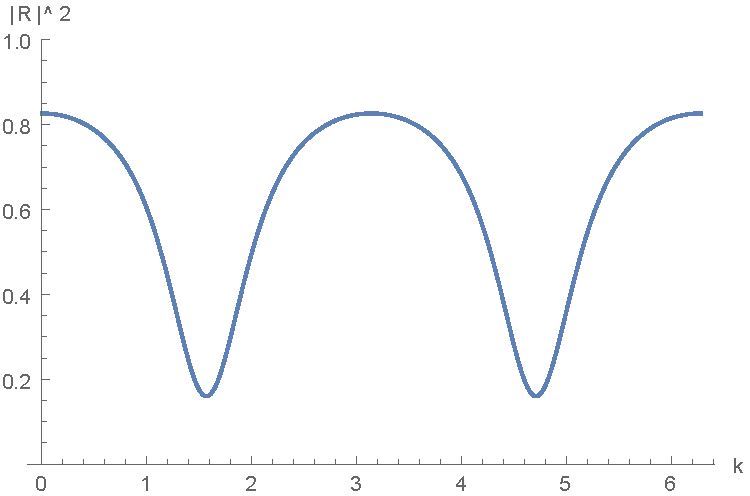
\includegraphics[width=1\textwidth]{img/2gen_reflection_l=1_b1=3_b2=7}
    \caption{$b_1=7, b_2=3$}
  \end{subfigure}
  \begin{subfigure}[t]{0.5\textwidth}
    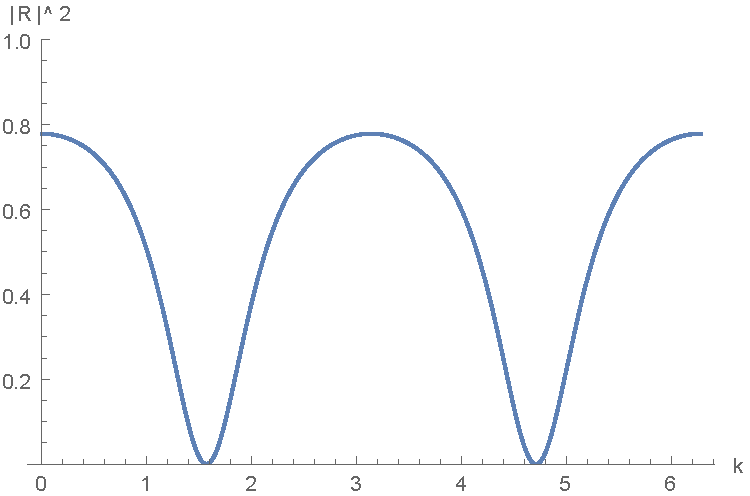
\includegraphics[width=1\textwidth]{img/2gen_reflection_l=1_b1=b2=4}
    \caption{$b_1=b_2=4$}
  \end{subfigure}
  \\
  \begin{subfigure}[t]{0.5\textwidth}
    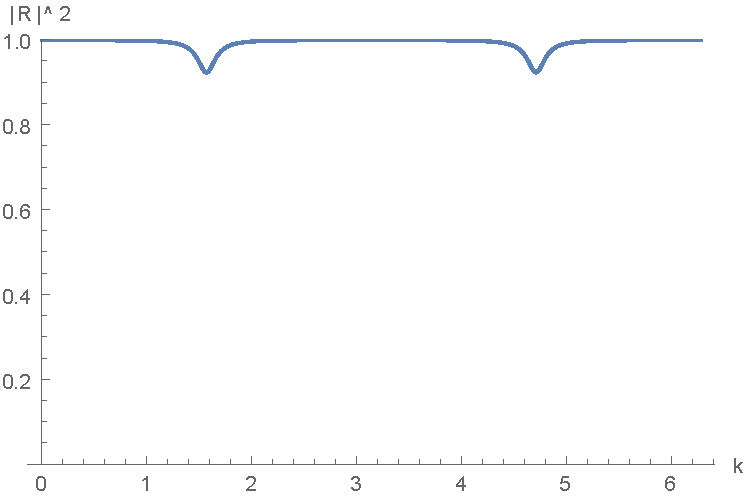
\includegraphics[width=1\textwidth]{img/2gen_reflection_l=1_b1=500_b2=10}
    \caption{$b_1=500, b_2=10$}
  \end{subfigure}
  \begin{subfigure}[t]{0.5\textwidth}
    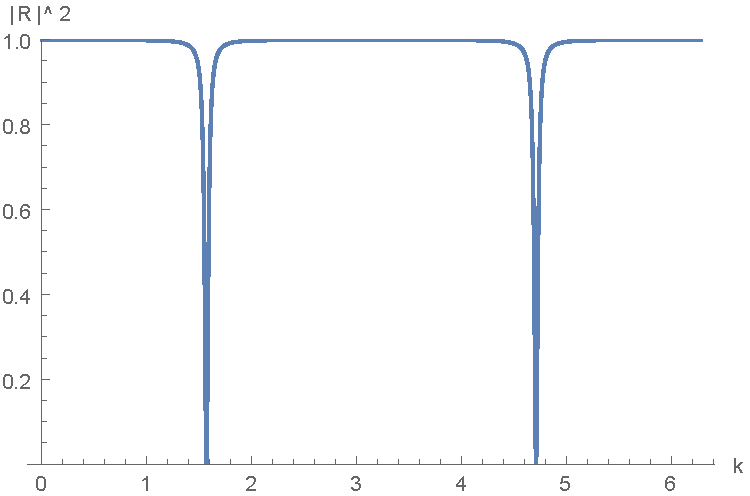
\includegraphics[width=1\textwidth]{img/2gen_reflection_l=1_b1=100_b2=100}
    \caption{$b_1=b_2=100$}
    \label{fig: 2 gen reflection gap}
  \end{subfigure}
  \caption{Reflection $\abs{R}^2$ from 2 generation radial quantum tree graph with inner edge length $\ell_1=1$ and varying branching numbers $b_1$ and $b_2$.}
  \label{fig: 2 gen reflection}
\end{figure}

Let us now consider what happens in the limiting case when one branching number grows large. As we have seen, $b_1$ and $b_2$ occurs symmetrically in the expression for $\abs{R}^2$. Hence we can without loss of generality keep $b_1$ fixed and let $b_2 \to \infty$, then from \eqref{eq: 2 gen reflection probability minimum} we see that the minimal reflection approaces 1, and thus $\abs{R} \to 1$ for all $k$. Similar to the case of the one generation radial quantum tree graph, we have the somewhat counterintuitive result that the probability of getting a reflection increases when the wave has more edges to propagate through. Keep in mind, though, that for $b_1 = b_2$ we always get zero reflection at the points $k = (2n+1)\pi/\ell_1, n = 1,2,3,\ldots$, but the interval for low reflection around these points gets smaller with increasing branching numbers, cf.\ figure~\ref{fig: 2 gen reflection gap}.

To continue this process for an arbitrary number $n$ of generations is unwieldy because one needs to calculate the determinant of a $2n \times 2n$ matrix. Instead, we will in the following chapter develop another method which makes the problem more tractable, and furthermore also gives a better insight into the scattering inside the graph.



% \section{Reflection from radial graphs with $n$ generations}

% General solutions to $Lu=u$ are
% \begin{equation}
%   \psi_j(x) = T_je^{ikx}+R_je^{-ikx}
% \end{equation}
% where $0\leq j\leq n$ is the generation number and $T_0=1, R_n=0$. The standard matching conditions give the system of equations
% \begin{equation}
%   \begin{dcases}
%     \psi_{j-1}(t_j) = \psi_j(t_j) \\
%     -\frac{d}{dx}\psi_{j-1}(t_j) + b_j\frac{d}{dx}\psi_j(t_j) = 0
%   \end{dcases}
%   \quad 1\leq j\leq n
% \end{equation}
% That is
% \begin{equation}
%   \begin{aligned}
%     % j=1: & \begin{cases}
%     %   e^{ikt_j} + R_{j-1} e^{-ikt_j} = T_j e^{ikt_j} + R_j e^{-ikt_j} \\
%     %   -ik(e^{ikt_j} - R_{j-1} e^{-ikt_j}) + b_j ik (T_j e^{ikt_j} - R_j e^{-ikt_j}) = 0
%     % \end{cases}\\
%     % 2\leq j\leq n-1: &
%     \begin{cases}
%       T_{j-1} e^{ikt_j} + R_{j-1} e^{-ikt_j} = T_j e^{ikt_j} + R_j e^{-ikt_j} \\
%       -ik(T_{j-1} e^{ikt_j} - R_{j-1} e^{-ikt_j}) + b_j ik (T_j e^{ikt_j} - R_j e^{-ikt_j}) = 0
%     \end{cases} \\
%     % j=n: & \begin{cases}
%     %   T_{j-1} e^{ikt_j} + R_{j-1} e^{-ikt_j} = T_j e^{ikt_j} \\
%     %   -ik(T_{j-1} e^{ikt_j} - R_{j-1} e^{-ikt_j}) + b_j ik T_j e^{ikt_j} = 0.
%     % \end{cases}
%   \end{aligned}
% \end{equation}
% As a matrix equation for 3 generations
% \begin{equation}
%   \begin{pmatrix}
%     -e^{-ikt_0}  & e^{ikt_0}      & e^{-ikt_0}       & 0              & 0                & 0             \\
%     ike^{-ikt_0} & b_0ike^{ikt_0} & -b_0ike^{-ikt_0} & 0              & 0                & 0             \\
%     0            & -e^{ikt_1}     & -e^{-ikt_1}      & e^{ikt_1}      & e^{-ikt_1}       & 0             \\
%     0            & -ike^{ikt_1}   & ike^{-ikt_1}     & b_1ike^{ikt_1} & -b_1ike^{-ikt_1} & 0             \\
%     0            & 0              & 0                & -e^{ikt_2}     & e^{ikt_2}        & e^{-ikt_2}    \\
%     0            & 0              & 0                & -e^{ikt_2}     & -b_2e^{ikt_2}    & b_2e^{-ikt_2} \\
%   \end{pmatrix}
%   \begin{pmatrix}
%     R \\ A \\ B \\ T_2 \\ R_2 \\ T
%   \end{pmatrix}
%   =
%   \begin{pmatrix}
%     e^{ikt_0} \\ ike^{ikt_0} \\ 0 \\ 0 \\ 0 \\ 0
%   \end{pmatrix}.
% \end{equation}


% Some observations

% \begin{itemize}
%   \item For 3 generations with equal edge lengths $\ell$ and equal branching numbers $m$ we get zero reflection iff
%   \begin{equation}
%     \cos 2k\ell = -\frac{1+m^2}{(1+m)^2}
%   \end{equation}
%   \item For any number of generations with equal length and branching number it appears to always be possible to get zero reflection.
%   \item With $m=2$ and 3 generations, zero reflection is given by at least $\ell_1=2\ell_2$ and $\ell_1=7\ell_2$, and symmetric between $\ell_1$ and $\ell_2$.
%   \item For 3 generations with equal branching number, $|R|^2$ is symmetric between the lengths.
% \end{itemize}


% \section{Minimal average reflection}


\clearpage

\chapter{The snowflake graph}\label{sec: snowflake}
\documentclass[a4paper,11pt]{report}

\usepackage[utf8]{inputenc}
\usepackage[T1]{fontenc}
\usepackage[hidelinks]{hyperref}
\usepackage[nottoc]{tocbibind}
\usepackage{caption}
\usepackage[labelformat=simple]{subcaption}
\renewcommand\thesubfigure{(\alph{subfigure})}

\usepackage{titlesec}

\usepackage{fancyhdr}


% Make section text look nice in header.
% (Only needed for article, not report.)
\makeatletter
\newcommand{\rightorleftmark}{%
  \begingroup\protected@edef\x{\rightmark}%
  \ifx\x\@empty
    \endgroup\leftmark
  \else
    \endgroup\rightmark
  \fi}
\makeatother

% hline in the footer, just like header.
\renewcommand{\footrulewidth}{0.4pt}

\pagestyle{fancy}
\renewcommand{\sectionmark}[1]{\markboth{\thesection~~~{#1}}{}}
\fancyhf{}
\lhead{\textsl{\rightorleftmark}}
\rhead{\thepage}
\lfoot{\textsc{Quantum Snowflake}}
\rfoot{\textsl{Viktor Qvarfordt}}
% \fancypagestyle{plain}{%
%   \fancyhf{}%
%   \renewcommand{\headrulewidth}{0pt}%
% }

\usepackage{mathtools,amssymb,amsthm,enumerate,cleveref}

\usepackage{tikz,tikzscale}
\usetikzlibrary{calc}

% Set up thm, def, etc.
\theoremstyle{plain}
\newtheorem{theorem}{Theorem}[chapter]
\newtheorem{proposition}[theorem]{Proposition}
\newtheorem{lemma}[theorem]{Lemma}
\newtheorem{corollary}[theorem]{Corollary}

\theoremstyle{definition}
\newtheorem{definition}{Definition}[chapter]
% \declaretheorem[name=Example,]{Ex}
\newtheorem{example}{Example}[chapter]
\AtEndEnvironment{example}{\hspace*{0pt}\hfill\ensuremath{\diamondsuit}}

\theoremstyle{remark}
\newtheorem{remark}{Remark}[chapter]

\numberwithin{equation}{chapter}

% \usepackage{showlabels}

\newcommand{\exclude}[1]{}

%% custom commands
\newcommand{\Dom}{\operatorname{Dom}}
\newcommand{\Ran}{\operatorname{Ran}}
\newcommand{\Ker}{\operatorname{Ker}}
\newcommand{\Tr}{\operatorname{Tr}}
\newcommand{\norm}[1]{\left\lVert#1\right\rVert}
\newcommand{\Norm}[1]{\lVert#1\rVert}
\newcommand{\abs}[1]{\left\lvert#1\right\rvert}
\newcommand{\ip}[2]{\ensuremath{\langle #1, #2 \rangle}}

\newcommand{\Z}{\mathbb{Z}}
\newcommand{\R}{\mathbb{R}}
\newcommand{\C}{\mathbb{C}}
\renewcommand{\H}{\mathcal{H}}

\newcommand{\D}[2]{\frac{d#1}{d#2}}
\newcommand{\pD}[2]{\frac{\partial#1}{\partial#2}}

\newcommand{\Dn}[3]{\frac{d^#3#1}{d#2^#3}}
\newcommand{\pDn}[3]{\frac{\partial^#3#1}{\partial#2^#3}}

\newcommand{\Dop}[1]{\frac{d}{d#1}}
\newcommand{\pDop}[1]{\frac{\partial}{\partial#1}}

\newcommand{\Dopn}[2]{\frac{d^#2}{d#1^#2}}
\newcommand{\pDopn}[2]{\frac{\partial^#2}{\partial#1^#2}}


\newcommand{\g}[1]{\left(#1\right)}


\title{Quantum Snowflake}
\author{Viktor Qvarfordt}


\begin{document}

\begin{titlepage}
  \thispagestyle{empty}
  % \null\vskip{-2em}
  % \noindent \large{\textbf{Stockholm University \hfill Fysikum}}
  % \vskip 7em
  \centering
  \null
  \vspace{3cm}
  {\huge\bf Quantum Snowflake} \\
  \vspace{1cm}
  {\Large\sl Viktor Qvarfordt} \\
  \vspace{0.5cm}
  {\Large May 2015} \\
  \vspace{4cm}
  {\Large Bachelor’s Thesis --- 15 ECTS} \\
  \vspace{0.5cm}
  \Large
  Supervisor: Pavel Kurasov \\
  \vspace{5cm}
  Department of Mathematics, Department of Physics \\
  \vspace{0.5cm}
  Stockholm University \\
  \vfill
  {\tiny Revised \today}
  \vspace{-1cm}
\end{titlepage}

\begin{abstract}
  Quantum graphs are defined and various general properties are explored. In particular, the Schrödinger equation is solved on the quantum snowflake graph, an infinite self-similar tree, in order to determine the graph's scattering properties. I.e.\ reflection and absorption for waves of varying energies that are sent into the snowflake graph are characterized.

By using the self-similarity and symmetries of the snowflake graph, a method is developed for reducing the snowflake graph to a line graph with special matching conditions. On this line graph, the complexity is further reduced by combining vertices into one meta-vertex. This procedure greatly simplifies the study of self-similar trees and gives a better understanding of the internal scattering of the graph.

Furthermore, it is shown that the periodic snowflake graph admits band gap structure, similar to crystalline materials. A recursive expression for the scattering coefficient for the general snowflake graph with $n$ generations is found.

\end{abstract}
% \thispagestyle{empty}
\clearpage

% \renewcommand{\abstractname}{Acknowledgments}
% \begin{abstract}
%   TODO

% \end{abstract}
% \thispagestyle{empty}
% \newpage

% \begin{figure}
%   \centering
%   \includegraphics[angle=90,width=\textwidth]{img/{snowflake_4_0.35_7_4_0.5}.pdf}
% \end{figure}

\fancypagestyle{snowflake}{\lhead{\textsl{Illustration of a quantum snowflake}}}
\thispagestyle{snowflake}
\setcounter{page}{3}
\begin{figure}
  \centering
  \includegraphics[width=\textwidth]{img/{snowflake_2_0.6_13_4_0.8}.pdf}
\end{figure}

\clearpage

{
\titleformat{\chapter}[display]{\normalfont\huge\bfseries}{\chaptertitlename~\thechapter}{20pt}{\Huge}
\titlespacing*{\chapter}{0pt}{-50pt}{25pt}
\tableofcontents
\clearpage
}

\chapter{Introduction}\label{sec: physical interpretation}\label{sec: introduction}
% \section{Preliminaries}

As the name suggests, quantum graphs model quantum mechanical particles on graph-like objects, edges joined in vertices. From a physical point of view, a quantum graph can be considered to be a network of thin (approximately one-dimensional) conductive wires on which quantum mechanical phenomena occur. On the graph, an electric and/or magnetic potential may be present. The main objective is to study how quantum mechanical particles---it is natural to consider electrons---propagate through the graph. The study of quantum graphs originated in 1930s as models for free electrons in molecules, and materials such as graphene have been modeled by quantum graphs.

% Note that we are not restricted to only quantum mechanics, in the sense that any wave-like phenomena described by sine and cosine functions or complex exponentials, such as waves in a fluid, can be modeled by the eigenfunctions of $L u = \lambda u$, where $L = - \Dopn{x}{2}$ and $\lambda$ represents the energy or frequency of the wave.

% Quantum graphs are studied both for their purely mathematical properties, and also because they are models for certain physical systems. Typical examples are systems that can be approximated as thin one-dimensional networks on which quantum mechanical phenomena occur. Indeed, quantum graphs originated as models for free electrons in molecules, and materials such as graphene have been modeled by quantum graphs.

Mathematically quantum graphs are defined as metric graphs, where edges are joined at vertices, along with a differential operator acting on functions defined on the metric graph. Most commonly one studies the eigenvalue problem of the magnetic Schrödinger operator
\[
  L_{q,a} = \g{i\Dop{x}+a(x)}^2+q(x).
\]
That is, one solves the time-independent Schrödinger equation
\[
  L_{q,a} \psi = \lambda \psi
\]
for a quantum mechanical particle living on the graph, where an electric potential $q(x)$ and magnetic potential $a(x)$ is applied. A metric graph is depicted in \cref{fig: basic quantum graph}.

\begin{figure}[h]
 \centering
  \begin{tikzpicture}[vertex/.style={draw,circle,minimum size=1.3mm,inner sep=0pt,outer sep=0pt,fill=black},scale=2, line width=0.8pt]
    \coordinate (p1) at (0,0);
    \coordinate (p2) at (1,0);
    \coordinate (p3) at (2,0);
    \coordinate (p4) at (2,1);
    \coordinate (p5) at (1.5,-0.5);
    \coordinate (p6) at (3,0.5);
    \coordinate (p7) at (2.75,-0.25);
    \coordinate (p8) at (0.75,0.75);
    % \coordinate (p9) at (3.5,0.5);
    \draw (p1)--(p2)--(p3)--(p4)--(p6);
    \draw (p2)--(p4);
    \draw (p3)--(p5);
    \draw (p2)--(p5);
    \draw (p3)--(p6);
    \draw (p3)--(p7);
    \draw (p2)--(p8);
    \draw (3.25,0.5) circle (0.25);
    \node[vertex] at (p1) {};
    \node[vertex] at (p2) {};
    \node[vertex] at (p3) {};
    \node[vertex] at (p4) {};
    \node[vertex] at (p5) {};
    \node[vertex] at (p6) {};
    \node[vertex] at (p7) {};
    \node[vertex] at (p8) {};
    % \node[vertex] at (p9) {};
  \end{tikzpicture}
  \caption{A graph.}
  \label{fig: basic quantum graph}
\end{figure}


For the equation to represent a physical system with real energies $\lambda$ one requires the operator $L_{q,a}$ to be self-adjoint. In particular this puts constraints on what can happen at the vertices, we must have certain matching conditions. The standard matching condition requires the functions to be continuous at every vertex, and in addition the sum of the outgoing derivatives from a vertex must be zero. This gives that the quantum probability of the wave is preserved after propagation through a vertex.

The purpose of this chapter is to bridge the gap between the point of view of readers more familiar with either mathematics or physics. We will introduce the aspects of quantum mechanics relevant for the study of quantum graphs and translate from the language of quantum mechanics to that of quantum graphs. More advanced concepts are deferred to the subsequent sections. In \cref{sec: defining quantum graphs} we properly define quantum graphs and further discuss metric graphs, differential operators, self-adjointness and matching conditions. In \cref{sec: properties} we explore various properties of quantum graphs and give several examples. All this builds up to \cref{sec: snowflake} where we introduce the snowflake graph, the central object of this thesis.

The quantum snowflake is defined as an infinite radial quantum tree graph that is also self-similar. By radial we mean that all properties of the graph, such as edge lengths and matching conditions, depend only on the distance from the root of the tree. The graph is self-similar in the sense that if one picks a vertex and cuts off the part of the graph that contains the root vertex, the remaining infinite subgraph is structurally identical to the original graph. In particular we require the length of every edge $e$ to be given by $\ell\beta^n$ where $n$ is the number of edges between $e$ and the root vertex, for $0<\beta<1$ we get a graph with finite depth $\ell/(1-\beta)$. On the graph we shall have standard matching conditions and no potentials.

The main objective will be to study the scattering properties of the quantum snowflake. Scattering phenomena is discussed in a more general context in \cref{sec: properties} and should be thought of as describing what information one can get out of a graph by physically examining it. To ``look'' at any object, in particular one described by a quantum graph, one shoots radiation, such as electrons, towards the object and observes how it scatters from the object. That is, we will characterize reflection and absorption for waves of varying energies that are sent into the snowflake graph.

We shall study the rotational symmetry of the snowflake graph, from which it will be possible to represent all eigenfunctions on the graph as a sum of quasi rotation invariant functions. This will allow us to collapse all edges in one generation into only one edge, from which the function values on all other edges can be reconstructed. Using this together with the self-similarity of the graph we can reduce the entire snowflake graph to a line graph with special snowflake matching conditions.

On the resulting line graph we shall further reduce the complexity by combining all vertices into one meta-vertex. This will lead to a recursive expression for the scattering coefficient for the general snowflake of $n$ generations.

This reduction of the graph greatly simplifies the study of the quantum snowflake and gives a better understanding of the internal scattering. It will be shown how the total scattering emerges from reflections on each edge of the graph.

As we will see, the general structure of the scattering from the snowflake graph is highly irregular. For the special case when the graph is periodic, i.e.\ all edges are of equal length, much more can be said. We shall show that the periodic snowflake gives rise to a band gap structure, similar to that of crystalline materials. This phenomena should be understood as arising from the fact that there exist energies that are not realizable inside the graph, therefore giving total reflection.

Finally the thesis is concluded with \cref{sec: conclusion} where we discuss of the obtained results and give indications for possible improvements and further research.




% \section{Physical interpretation}

% One should keep in mind that the mathematical models and assumptions ultimately stem from observations of nature, and can in principle not be derived mathematically. Oh really? Think about the Mathematical Universe Hypothesis.



\section{The Schrödinger equation}

It is well known that the Schrödinger equation describes the motion and behavior of quantum mechanical particles. The Schrödinger equation is often stated to be the result of empirical observations and therefore not possible to derive mathematically. However, one can arrive at the Schrödinger equation by starting from classical mechanics and imposing certain correspondence rules. In this section we motivate the Schrödinger equation by assuming that matter particles possess wave-like properties. By matter particle we mean the particles of which ordinary matter consists of, more specifically one may talk about fermions, the points is to distinguish from photons which we already know possesses wave-like properties. A more elaborate derivation of the Schrödinger equation starting from electromagnetic waves can be found in \cite{SE derivaiton}. There are indeed many ways to approach quantum mechanics and the Schrödinger equation, for instance quantization of classical mechanics or Feynman's path integral formulation, cf.\ \cite{feynman quantum mechanics}.

The following is a very naive derivation of the Schrödinger equation, illustrating how the equation arises from adding a wave-like property to classical particles, inspired by that of photons.

Let us consider a classical particle with mass $m$ and momentum $p$, the total energy is then $E = T + V$ where $T = \frac{p^2}{2m}$ is the kinetic energy and $V$ is the potential energy (from, say, an electric field) which we can leave unspecified, i.e.
\begin{equation}\label{eq: total energy}
  E = \frac{p^2}{2m} + V.
\end{equation}

We now introduce de Broglie's hypothesis, namely that matter particles possess wave-like properties just like photons. For photons we have the Planck--Einstein relation
\begin{equation}\label{eq: planck-einstein relation}
  E = h\nu
\end{equation}
relating the total energy $E$ to the frequency $\nu$ of the electromagnetic wave, where $h$ is Planck's constant. Furthermore, the energy--momentum relation states that
\begin{equation}\label{eq: energy-momentum relation}
  E^2 = (pc)^2 + (mc^2)^2
\end{equation}
for any particle, where $m$ is the intrinsic rest mass of the particle. Photons have no rest mass so this reduces to $E = pc$, where the velocity $c$ is given by $\lambda \nu$, where $\lambda$ is the wavelength. Using this we can combine the relations \eqref{eq: planck-einstein relation} and \eqref{eq: energy-momentum relation} to get
\begin{equation}\label{eq: de broglie relation}
  E = h \nu = pc = p \lambda \nu \iff p = \frac{h}{\lambda}.
\end{equation}
De Broglie's insight was that the wave-like property (which we are now introducing) of matter particles also obeys this relation, namely $p = h/\lambda$. The wavelength $\lambda$ is then interpreted as the wavelength of the matter wave associated with the particle, described by its wave function $\psi$. With no additional restrictions on the wave function it would take the general form of d'Alembert waves
\[ \psi(x, t) = f(x - vt) + g(x + vt) \]
but we will for now consider the case of simple plane waves
\[ \psi(x, t) = Ae^{i(kx - \omega t)} + Be^{i(-kx - \omega t)}. \]
(Plane waves corresponds to freely propagating waves, we will see more on this in section~\ref{sec: stationary states}.)
The wave number $k$ is related to the wavelength $\lambda$ by $k = \frac{2\pi}{\lambda}$. Using the de Broglie relation \eqref{eq: de broglie relation} we then have
\begin{equation}\label{eq: k-p relation}
  k = \frac{p}{\hbar}
\end{equation}
where $\hbar = \frac{h}{2\pi}$ is the reduced Planck constant.
Differentiating $\psi$ with respect to the spatial coordinate gives
\[ \pD{\psi}{x}(x, t) = ik\psi(x, y) = i\frac{p}{\hbar} \psi(x, t), \]
hence we have the momentum operator relation
\[ p = -i\hbar\pDop{x}. \]
We only see that this holds for plane waves $\psi(x, t) = Ae^{i(kx - \omega t)} + Be^{i(-kx - \omega t)}$, but this is indeed a general result.
Now, we can write equation \eqref{eq: total energy} as
\begin{equation}\label{eq: tise}
  E \psi = -\frac{\hbar^2}{2m}\pDn{\psi}{x}{2} + V\psi.
\end{equation}
We have arrived at the time-independent Schrödinger equation, TISE.

Furthermore, if we relate $E$ to the temporal frequency $\frac{\omega}{2\pi}$ of the wave function via the Planck--Einstein relation \eqref{eq: planck-einstein relation}---which we can use since we have assumed a wave-like property matter particles similar to that of photons---we have
\[ E = \hbar \omega. \]
Differentiating $\psi$ with respect to the temporal coordinate, and using the above relation, gives
\[ \pD{\psi}{t}(x,t) = -iw\psi(x,t) = \frac{-iE}{\hbar} \psi(x,t), \]
that is
\begin{equation}
  E\psi(x,t) = i \hbar \pD{\psi}{t}(x,t).
\end{equation}
Substituting this for the left hand side in the time-independent Schrödinger equation \eqref{eq: tise} gives
\begin{equation}\label{eq: tdse}
  i \hbar \pD{\psi}{t} = -\frac{\hbar^2}{2m}\pDn{\psi}{x}{2} + V\psi,
\end{equation}
the time-dependent Schrödinger equation, TDSE.

In our example we can introduce the Hamiltonian $H$ as the operator defined by the expression
\[ H = \widehat{T} + \widehat{V} = -\frac{\hbar^2}{2m}\pDopn{x}{2} + V(x) \]
where
\[ \widehat{T} = -\frac{\hbar^2}{2m}\pDopn{x}{2} = \frac{\widehat{p}^2}{2m} \]
is identified as the kinetic energy operator with
\[ \widehat{p} = -i \hbar \pDop{x} \]
being the momentum operator and $\widehat{V} = V(x)$ is the potential energy operator. The TDSE can then be written more compactly as
\[ i\hbar \pD{\psi}{t} = H\psi \]
and the TISE becomes an eigenvalue equation for the operator $H$
\[ H\psi = E\psi. \]
The Hamiltonian recovered above is the usual Hamiltonian for a particle propagating under the influence of a potential $V(x)$, but for other particular systems the Hamiltonian may take another form.
If we use natural units where $\hbar=1$ and let the $m = 1/2$, so that $\frac{\hbar^2}{2m} = 1$, and denote the energy in these normalized units by $\lambda$, then the TISE for the usual Hamiltonian can be written as
\[ L_q\psi = \lambda\psi. \]
That is $H = L_q$ where $L_q$ was defined in \eqref{eq: magnetic schrödinger operator}. The magnetic potential is taken into account by letting
\[ \widehat{p} = -i \pDop{x} - a(x), \]
then $H = L_{q,a}$. In the subsequent sections we will only use normalized units, as described above.



\section{Quantum states and interpretations of quantum mechanics}\label{sec: quantum states and interpretations of quantum mechanics}

Classically, properties of an object, or the \emph{state} of an object, is characterized by its position and momentum. In quantum mechanics the state of a particle is instead specified by its wave function, containing information about both the position and momentum of the particle. The Schrödinger equation gives the possible such states, their corresponding energies, and how they evolve over time.

A fundamental property of quantum mechanics is that quantities such as energy for a particle can be constrained to discrete values, for example the energy of an electron bound to an atom. However, a freely propagating electron can take energies from a continuous spectrum. Recall from section~\ref{sec: spectrum} that the spectrum of linear operators may have this property, namely the spectrum can be both discrete and continuous. It is therefore a postulate of quantum mechanics that to each dynamical variable, ``observable'', there corresponds a linear operator such that all possible values of the variable are given by the spectrum of the operator.

The \emph{ground state energy} (zero-point energy) is the lowest positive eigenvalue $\lambda_0$, the higher eigenvalues are called excited state energies.

% For many graphs also $\lambda = 0$ is an eigenvalue, however this energy is not physically realizable because of the uncertainty principle. As can be shown, the wave function $\psi(x)$ in position space and wave function $\widetilde{\psi}(p)$ in momentum space are Fourier transform duals of each other. Hence we have $\sigma_x\sigma_p \le 1$, where $\sigma_a$ denotes the standard deviation of a variable $a$, (the lower bound depends on which particular definition of the Fourier transform that is being used, and what units we assume). From this we see that $E=0$ is not possible, since this is implies zero kinetic energy, i.e.\ zero momentum, hence $E>0$.

The statistical interpretation of quantum mechanics, introduced by Max Born in \cite{born statistical interpretation}, originally motivated entirely by observation, states that the probability of observing a quantum mechanical particle at a particular location $x$ and time $t$ is given by the probability density function $\abs{\psi(x,t)}^2$, this fact is known as the Born rule.
% This also exemplifies why one requires $\psi \in L^2$, so that the total probability equals unity.

Although this thesis primarily deals with the mathematical properties of quantum graphs, we will broaden our view of the physical significance of the mathematics and highlight questions that arise when interpreting the models by making a slight detour into the interpretation of quantum mechanics, by discussing the so called measurement problem.

Quantum mechanical particles are often spread out in space, in the sense that $\psi(x)$ is non-zero on some interval (in fact, time evolution tends to smear out the wave function), while on the other hand, a measurement of the position of a particle always yields a specific position, in accordance with the Born rule. The wave-like property can only be implicitly detected by studying interference of the wave function.
% In the context of quantum graphs, the stationary states of any graph have a wave function that is non-zero almost everywhere on the entire graph, while any attempt to measure the position of the particle will yield a specific position.

This seemingly collapse of the wave function, from being smeared out to becoming highly localized, is not in any way described by the mathematics of quantum mechanics. The text-book approach of describing this is by adding a postulate to the model, namely that the wave function collapses (i.e.\ becomes highly localized) to the measured value. This is what is known as the Copenhagen interpretation. This interpretation arguably has several issues, for example, what precisely constitutes a measurement? Any interaction of particles is in a sense a measurement. Einstein's objection is often quoted as ``God does not throw dice'', pointing out that the random collapse of the wave function is ill-justified and not consistent with our otherwise deterministic model of reality. Other so called collapse theories exist, perhaps most noteworthy is the Ghirardi--Rimini--Weber theory, postulating that the wave function undergoes spontaneous collapse and random yet very frequent points in time. This avoids the problem of what denotes a measurement in the Copenhagen interpretation while still giving predictions that are in agreement with observations.

Any collapse theory will necessarily contain fundamental randomness. This may seem unavoidable if the Born rule is to be satisfied, but this is not the case. The mathematically simplest interpretation is to not add any additional postulates, contrary to the other interpretations, that is to say that the wave function never collapses, it continues to evolve deterministically according to the Schrödinger equation. In this interpretation every measurement entangles the ``observer'' to the measured system, thus entering a superposition state. Measurements are then not distinguished from any other form of interaction between particles, unlike in the Copenhagen interpretation.

This entails that the entire environment gets entangled to the quantum state being measured, from which the classical state emerges as an apparent collapse of the wave function, an effect called decoherence. In this interpretation every possible classical state exists in a superposition. This gives rise to the Many Worlds Interpretation originally introduced by Hugh Everett, in which, by the effect of decoherence, non-interacting branches of the wave-function (and in extension reality) get created. The Born rule is then an emerging property in every decohered slice of reality \cite{carroll EQM probability, wallace born rule}.

One may argue that the interpretation is not important, since all interpretations give equal predictions, but this is not necessarily the case. There are contrived gedanken experiments for which, for example, collapse theories and the many world theory gives different predictions \cite{vaidman mwi}.

A radically different approach is Quantum Bayesianism, in which one assumes that quantum states do not represent elements of physical reality \cite{qbism introduction, qbism and the greeks}. This is a rather pragmatic approach in which quantum mechanics is merely a tool for making statistical predictions, in this way avoiding the problematic implications of interpreting quantum states as representations of physical reality.

Towards the other extreme we have the Mathematical Universe Hypothesis by Max Tegmark \cite{tegmark}, essentially extending from the Many worlds interpretation, postulating that the physical world is an abstract mathematical structure. Hence stating that quantum states truly are elements of physical reality (provided that quantum mechanics is a correct description of reality).

There is no consensus on how quantum mechanics is to be interpreted, and the discussion quickly becomes philosophical. There is however no doubt in that it is a very successful theory in the sense that all predictions so far are in perfect agreement with empirical results.
% In what follows we will generally not be concerned with interpretations and when necessary we will apply the Born rule without further ado.



\section{Stationary states}\label{sec: stationary states}

Stationary states are states that do not evolve over time, in the sense that $\abs{\psi(x,t)}^2$ is constant in $t$, stationary. This allows for a time dependence of the probability amplitude $\psi(x,t)$ only as a phase shift $e^{i\theta(t)}$, where $\theta(t) \in \R$. As we will see in equation \ref{eq: time-separated solution}, the phase is given by $\theta(t) = -\lambda t$. Stationary states are important since they are the states of equilibrium, states reached after some time when the system has settled.
% The study of quantum graphs mainly focuses on such states.
% General solutions to the Schrödinger equation can be expressed as a series of stationary states, therefore most attention is directed towards stationary states.
Considering only stationary states greatly simplifies matters, since the TISE is an ordinary differential equation while the TDSE is a partial differential equations. On the other hand, every solution to the TDSE can be written as a superposition of stationary states, showing that it is essentially sufficient to consider such states.

The stationary solutions to the time-dependent Schrödinger equation \eqref{eq: tdse} can be found by using separation of variables with the Ansatz
\[ \psi(x,t) = u(x) T(t). \]
This then gives, with $q(x) \equiv a(x) \equiv 0$ for convenience,
\[
  i \Dop{t} u(x) T(t) = - \Dopn{x}{2} u(x) T(t) \iff
  i \frac{\D{T}{t}(t)}{T(t)} = - \frac{\Dn{u}{x}{2}(x)}{u(x)} = \lambda,
\]
for some constant $\lambda$. That is,
\begin{align*}
  i \D{T}{t}(t) &= \lambda T(t) \\
  - \Dopn{x}{2}u(x) &= \lambda u(x).
\end{align*}
The second equation is precisely the time-independent Schrödinger equation for the spatial component $u(x)$, justifying that the constant $\lambda$ is to be interpreted as the energy of the system (in normalized units). With $k^2 = \lambda$ we can write the solutions for $u(x)$ as
\[ u(x) = Ae^{ikx} + Be^{-ikx} \]
and the solution for the time component $T(t)$ as
\begin{equation}\label{eq: time-separated solution}
  T(t) = e^{-i\lambda t}.
\end{equation}
Hence the solution to the TDSE is given by
\begin{equation}\label{eq: left right waves}
  \psi(x,t) = Ae^{i(kx-\lambda t)} + Be^{i(-kx-\lambda t)},
\end{equation}
showing that the two terms can be interpreted as right and left traveling waves, respectively. The constants $A$ and $B$ and possible values of $\lambda$ are to be determined by the particular situation, see for instance example~\ref{ex: particle in a box}.

The wave function of a stationary state is given by standing waves, evolving in time only by changing the phase shift.

The criteria of $H$ being self-adjoint, discussed in \ref{sec: differential operators}, is important in the quantum mechanical interpretation. It ensure that the model is physical in the sense that the eigenvalues of $H$ are real, which is necessary since this represents the energy of the system. Furthermore, the eigenvectors of $H$ are then orthogonal and can be chosen so that they form an orthonormal basis of the state space. This, together with the linearity of the equation, allows any solution of the TDSE to be written as a linear combination of stationary states, showing that it is sufficient, without loss of generality, to consider only the stationary states.



\clearpage

\fancypagestyle{automatic}{\lhead{\textsl{\rightorleftmark}}}
\pagestyle{automatic}

\chapter{Defining quantum graphs}\label{sec: defining quantum graphs}
This section is devoted to defining and discussing quantum graphs and the components that it consists of. A more thorough introduction and characterization of quantum graphs can be found in the survey article \cite{introduction and brief survey} or the books \cite{pavel book} and \cite{berkolaiko kuchment book}. We begin by defining exactly what is meant by a quantum graph. The meaning of the terms will be explained in the following sections.

\begin{definition}
  A \emph{quantum graph} is a triple $(\Gamma, L, \text{MC})$, where
  \begin{itemize}
    \item $\Gamma$ is a \emph{metric graph},
    \item $L$ is a \emph{differential expression} defined on a function space on $\Gamma$, and
    \item MC is a set of equations, \emph{matching conditions}, relating the limit values  of the functions defined on the edges of $\Gamma$.
  \end{itemize}
\end{definition}

Similar to how, in abstract algebra, one talks about a group $(G,*)$ by referring to its underlying set $G$, we will often talk about a given quantum graph $(\Gamma, L, \text{MC})$ by referring to the metric graph $\Gamma$, often called the \emph{underlying (metric) graph}.

Initially the quantum graph is only given a differential expression $L$. Next, one defines a corresponding differential operator whose action is given by the differential expression, furthermore one must determine the domain of the operator, so that the operator satisfies desired properties such as being self-adjoint. The domain of the operator is not known \textit{a priori}, therefore we only include a differential expression in the definition of a quantum graph.
% Usually one chooses $L$ so that the eigenvalue problem $L\psi=\lambda\psi$ is the Schrödinger equation, or some other equation of interest.
The three components in the definition are dependent of each other in the sense that one often defines the underlying metric graph from the geometry of the problem. The differential operator is then defined as acting on functions defined on the edges of this graph, satisfying the matching conditions to ensure self-adjointness and other properties of interest.

As we will see in \cref{sec: snowflake}, two graphs of different geometry, i.e.\ having different underlying metric graphs, can be equivalent by a certain choice of matching conditions for the ``geometrically altered'' graph. This turns out to be a powerful method of simplifying studies of more complicated graphs.

It is natural to begin our discussion with metric graphs, which we now proceed to define.



\section{Metric graphs}\label{sec: metric graphs}

In discrete mathematics, combinatorial graphs are defined as vertices connected to each other through edges. The edges merely reflect the relation between vertices, which are the main objects of the graph. Metric graphs can then be defined as combinatorial graphs with weights assigned to each vertex, but it is useful to change the point of view slightly.

In contrast to combinatorial graphs, the main objects of metric graphs are the edges, while the vertices merely reflect the relation between edges. Let us now formally define a metric graph, note how we still have vertices and edges, but they play a very different role.

\begin{definition}
  A \emph{metric graph} is a tuple $(E,V)$ where
  \begin{itemize}
    \item $E = \{e_n\}_{n=1}^N$ is a set of intervals $[x_{2n-1}, x_{2n}] \subset \R$ called \emph{edges}, where $x_{2n-1} < x_{2n}$. At least one end-point of each interval must be finite. If both end-points are finite then the edge is called compact, otherwise it is called semi-infinite.
    \item $V = \{v_m\}_{m=1}^M$ is a partition of the set of all end-points of edges in $E$, each element in $V$ is called a \emph{vertex}. End-points belonging to the same vertex (partition) are identified as the same point.
  \end{itemize}
\end{definition}

It is this construction of the vertices that defines the connection between the otherwise completely independent edges in $E$. The partition of endpoints into vertices, or the equivalence relation giving rise to it, can thus be viewed as defining the geometry of the graph, or vice versa.

It is useful to think of metric graphs as intervals of the real line, being the edges, joined together at some of their end-points, being the vertices. The physical interpretation could then be thin metal wires welded together at some points, we will come back to this after we have introduced the differential operator acting on the graph.

Similar to combinatorial graphs, we define the \emph{degree} $\deg v_m$ of a vertex $v_m$ to be the number of edges connected through this vertex. Equivalently it is the number of edges containing the vertex, i.e.\ the degree is simply $\abs{v_m}$, the number of end-points belonging to the vertex.

A metric graph $\Gamma$ is said to be connected if there exists a continuous path in $\Gamma$ connecting $x$ and $y$ for every $x, y \in \Gamma$. If this does not hold for every $x$ and $y$ the graph is considered to be split into a number of disconnected subgraphs or connected components, each being a connected graph containing at least one edge. If a graph has several connected components, they can be considered to be completely independent graphs, in this text we shall only be interested in connected graphs.

Unlike combinatorial graphs, edges $e_n$ in metric graphs have the notion of length, simply defined as $\ell_n = x_{2n} - x_{2n-1}$. From this we can define the total length of a graph as $\mathcal{L} = \sum_{n=1}^{N} l_n$. We also introduce a distance $d(x, y)$ between any two points $x$ and $y$ in a connected metric graph as the length of the shortest path between $x$ and $y$.

We now define what is meant by a function being defined on the graph, we often consider functions from the following functions spaces.

\begin{definition}[Function spaces on metric graphs]
  Let $\Gamma$ be a metric graph, the Hilbert space $L_2(\Gamma)$ is then the direct sum of the $L_2$ spaces on each edge of $\Gamma$. That is the set of all functions that are square integrable on each edge:
  \[
    L_2(\Gamma) = \bigoplus_{e \in E} L_2(e).
  \]
  Similarly we define the Sobolev space $W_2^2(\Gamma\setminus V)$ as the set of all square integrable functions with weak derivatives up to order 2 being square integrable:
  \[
    W_2^2(\Gamma\setminus V) = \bigoplus_{e \in E} W_2^2(e).
  \]
  Analogously we define $C^\infty_0(\Gamma\setminus V)$ as the set of smooth functions with support separated from the vertices of $\Gamma$.
\end{definition}

We will also need the notion of inner product between two functions on the graph.

\begin{definition}[$L_2$ inner product and norm on metric graphs]\label{def: inner product on graph}
  The $L_2$ inner product on a metric graph $\Gamma$ is given by
  \[
    \ip{f}{g}_{L_2(\Gamma)} =
    \sum_{e \in E} \ip{f}{g}_{L_2(e)} =
    \sum_{e \in E} \int_e f(x)\overline{g}(x)\,dx
  \]
  which we can write as $\int_\Gamma f(x)\overline{g}(x)\,dx$, where $\overline{z}$ denotes complex conjugation of $z$.
  The $L_2(\Gamma)$ norm is then naturally defined by
  \[
    \norm{f}_{L_2(\Gamma)} = \ip{f}{f}_{L_2(\Gamma)} = \int_{\Gamma} \abs{f(x)}^2 dx.
  \]
\end{definition}

These definitions are very natural generalizations of the same concepts on intervals of $\R$, further adding to the notion that metric graphs are merely sets of intervals of $\R$ that share some end-points.

A function $f$ defined on $\Gamma$ is simply a function defined independently on each edge. This leads to the problem of $f(x_j)$ not being well defined where $x_j \in v$ for some vertex $v$. Points in $v$ are by definition identified as the same point but the definition of $f$ does not reflect this. If $f$ is continuous on each edge we can define $f(x_j)$ as
\begin{align*}
  f(x_{2n}) &= \lim_{x \to x_{2n}^-} f(x) \\
  f(x_{2n-1}) &= \lim_{x \to x_{2n-1}^+} f(x),
\end{align*}
that is, the limits are taken as one-sided limits from the inside of the edge. Later we will consider functions continuous on the entire graph, in which case even $f(v)$ will be well defined.

As we've seen it is natural to consider limits at a vertex as the one-sided limit taken from inside the edge. Motivated by this we introduce the following.

\begin{definition}
  The \emph{normal derivative} $\partial f(x_j)$ of a function $f$ on a metric graph $\Gamma$ at an end-point $x_j$ of an edge is given by
  \begin{align}
    \partial f(x_j) =
    \begin{dcases}
      \lim_{x \to x_j}   \Dop{x} f(x) & j = 2n-1 \\
      \lim_{x \to x_j} - \Dop{x} f(x) & j = 2n
    \end{dcases}
  \end{align}
\end{definition}

This should be understood as taking the derivative in the direction into the edge, out from the vertex given by the end-point $x_j$. This is a useful concept since it allows us to disregard the direction of parametrization of the edge. For this graph it is indeed only the length of an edge that is of relevance, in section~\ref{sec: edge parametrization} we will consider how edge parametrization affects graphs in general.



\section{Differential operators}\label{sec: differential operators}

We now introduce the differential operator acting on function from the function space of the underlying metric graph. The differential operator can be seen as defining which phenomena is being studied on the graph. The most simple and common operator is the \emph{Laplace operator}
\begin{equation}\label{eq: laplacian}
  L = - \Dopn{x}{2}.
\end{equation}
Note that the domain of the operator must be carefully defined, as we shall see in section~\ref{sec: self-adjoint operators}, the domain plays a very important role for properties of the operator, such as self-adjointness. Until then, let us consider the simple case $\Dom L = C^2(\R)$, in order to get a preliminary understanding of the operators that will come into play. The eigenfunctions $u(x)$ of $L$, satisfying
\[ Lu = \lambda u, \] are complex waves which can be written as
\[ u(x) = Ae^{ikx} + Be^{-ikx}, \quad k^2 = \lambda. \]
Solving the eigenvalue problem $Lu=\lambda u$ amounts to studying wave propagation through one-dimensional structures connected at the vertices, being the graph $\Gamma$. In order to do this properly we must define matching conditions at the vertices, as we shall do in section~\ref{sec: mc}.

Because of the relation
\[
  Ae^{ikx} + Be^{-ikx} = C\cos kx + D\sin kx
\]
for complex constants $A, B, C$ and $D$ such that $C=A+B$ and $D=i(A-B)$, we can chose to represent the eigenfunctions of $L$ as complex exponentials or trigonometric functions. We will see that in different contexts one representation may be more convenient than the other. If one wants to emphasize the evenness or oddness of the eigenfunction, c.f.~\ref{ex: even odd eigenfunctions}, the trigonometric representation is superior. On the other hand the complex exponential form splits the eigenfunction into left and right traveling waves, c.f.~\ref{eq: left right waves}.

More generally one introduces the \emph{Magnetic Schrödinger operator}
\begin{equation}\label{eq: magnetic schrödinger operator}
  L_{q,a} = \left(i\Dop{x} + a(x)\right)^2 + q(x)
\end{equation}
where $a(x)$ is the magnetic potential and $q(x)$ is the electric potential present on the graph. With no magnetic potential we denote $L_{q,0} = L_q$ simply as the \emph{Schrödinger operator}. Note also that $L_{0,0} = L$. The eigenfunctions of $L_{q,a}$ describe the stationary states of quantum mechanical particles on the graph under the influence of electric and magnetic potential. In particular, $L_q \psi = \lambda \psi$ is the standard time-independent Schrödinger equation, see \cref{sec: physical interpretation} for more details on the physical interpretation.

Before we proceed we shall formalize the notion of operators and consider some of their properties.
% We outline only the basics and important notions that will later be used. More information can be found in any book on functional analysis.


\subsection{Operator formalism}

Let us first recall that an operator $A$ is a mapping between two linear vector spaces $X$ and $Y$ with scalars in $\C$,
\[ A : X \to Y. \]
The operator is said to be linear if $A(\alpha x + \beta y) = \alpha A x + \beta A y$ where $x,y \in X$ and $\alpha, \beta \in \C$.
We shall mostly be concerned with the case when $X$ and $Y$ are function spaces, such as the introduced Sobolev space $W_2^2(\Gamma\setminus V)$. In this case we write $(Af)(x)$, i.e. $A$ operates on a function $f \in X$ and gives a function $Af \in Y$, which in turn is applied to an element $x$ from the domain of functions in $Y$.
Composition $(ABf)(x)$ of two operators $A$ and $B$ is to be understood as $A(B(f(x)))$.
The following example shows how to work with operator expressions and that, in general, operators do not commutative.

\begin{example}
  Let $A$ and $B$ be two operators defined on the same function space, the equation
  \[ A = B \]
  should be understood as
  \begin{enumerate}[i)]
    \item $\Dom A = \Dom B$
    \item $Af = Bf$ for every function $f$ in the domain.
  \end{enumerate}
  The importance of this is exemplified by considering the operators
  \[ A = \Dop{x}, \quad B = g(x), \]
  where $A$ is the derivative operator and $B$ is simply pointwise multiplication by a continuously differentiable function $g(x)$. Let the domain of both operators be $C^1(\R)$. It is not true that
  \begin{equation*}
    AB = \frac{d}{dx}g(x) = g'(x),
  \end{equation*}
  which is clear if we let $AB$ act on a function
  \begin{align*}
    (ABf)(x) &= \big(A(Bf)\big)(x) \\
    &= \frac{d}{dx}\Big(g(x)f(x)\Big) \\
    &= g'(x)f(x)+g(x)f'(x) \\
    &= \left(g'(x)+g(x)\Dop{x}\right)f(x).
  \end{align*}
  That is,
  \[ AB = g'(x)+g(x)\frac{d}{dx}, \]
  which shows that caution must be exercised when dealing with operator expressions.
  On the other hand we have
  \[ (BAf)(x) = g(x)f'(x), \]
  showing that
  \[
    BA = g(x)\Dop{x}
  \]
  In conclusion we have that the commutator between $A$ and $B$ is given by
  \[
    AB-BA = g'(x).
  \]
\end{example}

We now state some important definitions.

\begin{definition}[Bounded operator]
  An operator $A: X \to Y$ is said to be \emph{bounded} if there exists a constant $C$ such that
  \[
    \norm{Ax} \le C \norm{x} \quad \forall x\in X.
  \]
  Furthermore, the infimum over all such constants $C$ is called the \emph{norm} of $A$, denoted by $\norm{A}$. If no such $C$ exists, we say that $A$ is unbounded.
\end{definition}

\begin{definition}[Isometric operator]
  An operator $A: X \to Y$ is said to be \emph{isometric (norm preserving)} if
  \[ \norm{Ax}_Y = \norm{x}_X \quad \forall x \in X. \]
\end{definition}

\begin{definition}[Unitary operator]
  An operator $A: X \to Y$ is said to be \emph{unitary} if it is defined on the whole space $X$, is isometric and surjective. In particular this gives that $A$ is invertible and
  \[ AA^* = A^*A = I. \]
\end{definition}

To properly define an operator $L: X \to Y$, its domain $\Dom(L) \subseteq Y$ must be specified. As it turns out, the domain of an operator plays a very important role for the properties of the operator.

\begin{example}[Shift operator]
  Consider the space $\ell^2$ consisting of all infinite sequences $\vec{x}=(x_1, x_2, \ldots)$ with
  \[
    \norm{\vec{x}}_2 = \sqrt{\sum_{n=1}^{\infty} \abs{x_n}^2} < \infty.
  \]
  Define the \emph{shift operator} $S$ on $\ell^2$ by
  \[
    S(x_1, x_2, \ldots) = (0, x_1, x_2, \ldots).
  \]
  Clearly $S$ is an isometry, the norm of $\vec{x}$ is preserved for every $\vec{x} \in \ell^2$:
  \[
    \norm{S(\vec{x})}
    = \norm{(0,x_1,x_2,\ldots)}
    = \sqrt{\sum_{n=1}^{\infty} \abs{x_n}^2 }
    = \norm{(x_1, x_2, \ldots)}
    = \norm{\vec{x}}.
  \]
  However, $\Ran S \ne \ell^2$ since any element $\vec{x} = (x_1, x_2, \ldots)$ with $x_1 \ne 0$ is not contained in $\Ran S$. Hence, the shift operator $S$ is not surjective and thus not unitary.
\end{example}




\subsection{Self-adjoint, symmetric and hermitian operators}\label{sec: self-adjoint operators}

\begin{quote}\itshape
  ``In the 1960s Friedrichs met Heisenberg, and used the occasion to express to him the deep gratitude of the community of mathematicians for having created quantum mechanics, which gave birth to the beautiful theory of operators in Hilbert space. Heisenberg allowed that this was so; Friedrichs then added that the mathematicians have, in some measure, returned the favor. Heisenberg looked noncommittal, so Friedrichs pointed out that it was a mathematician, von Neumann, who clarified the difference between a self-adjoint operator and one that is merely symmetric. `What's the difference', said Heisenberg.'' \normalfont\cite[p.~414]{lax}
\end{quote}

As the quote above indicates, there is often confusion regarding the concepts of self-adjoint, symmetric and hermitian operators. The topic of functional analysis, operator theory and in particular unbounded self-adjoint operators is deep, and we shall only touch upon the topics directly related to the study of quantum graphs, further details can be found in \cite{teschl-fa, teschl-schroe, schmudgen}. What is presented below is mainly taken from \cite[section 1.2]{schmudgen} and \cite[section 5.1]{pedersen}. Recall first that a Hilbert space is a complete inner-product space.
% The difficulty arises when the operator is unbounded, which also is the most interesting case since the operators $L_{q,a}$ we are working with are unbounded operators.

Let $\H_1$ and $\H_2$ be Hilbert spaces and let $T$ be a linear operator from $\H_1$ to $\H_2$ such that the domain $\Dom T$ is a linear subspace that is dense in $\H_1$, that is $\overline{\Dom T} = \H_1$ where $\overline{\Dom T}$ denotes the closure of $\Dom T$. Set
\[
  \Dom T^* = \{y \in \H_1 \mid \text{the functional } x \mapsto \ip{Tx}{y}_2 \text{ on } \Dom T \text{ is bounded} \}.
\]
Since $\Dom T$ is dense in $\H_1$, the functional $x \mapsto \ip{Tx}{y}_2$ extends by continuity to $\H_1$ (a linear functional is bounded if and only if it is continuous \cite[theorem 4.4.2]{friedman}). By Riesz's theorem \cite[theorem 6.2.4]{friedman} there exists a unique element $z \in \H_1$ such that $\ip{Tx}{y}_2 = \ip{x}{z}_1$. Hence we can set $T^*y = z$ to obtain a well-defined mapping $T^*$ from $\H_1$ to $\H_2$, and we have
\begin{equation}\label{eq: adjoint symmetric relation}
  \ip{Tx}{y}_2 = \ip{x}{T^*y}_1 \quad \forall x \in \Dom T, \; y \in \Dom T^*.
\end{equation}

\begin{definition}[Adjoint operator]
  Let $T$ be a densely defined linear operator from $\H_1$ to $\H_2$, both being Hilbert spaces.
  The operator $T^*$ as described above is called the \emph{adjoint} operator of $T$.
\end{definition}

If $S$ and $T$ are two linear operators from $\H_1$ to $\H_2$ we say that $S = T$ if and only if their domains coincide, i.e.\ $\Dom S = \Dom T$, and additionally $S(x) = T(x)$ for all $x$ in the domain. If $\Dom S \subseteq \Dom T$, and if the operators agree on the common domain, that is $S(x) = T(X)$ for all $x \in \Dom S$, then we say that $S$ is a restriction of $T$ or equivalently that $T$ is an extension of $T$, and write $S \subseteq T$.

\begin{definition}[Symmetric operator]
  Let $T$ be a densely defined linear operator on a Hilbert space, then $T$ is called \emph{symmetric} if $T \subseteq T^*$.
\end{definition}

\begin{definition}[Self-adjoint operator]
  Let $T$ be a densely defined linear operator on a Hilbert space, then $T$ is called \emph{self-adjoint} if $T = T^*$.
\end{definition}

% \begin{definition}[Symmetric operator]
%   An operator $T$ defined on a Hilbert $\H$ space is called symmetric if
%   \[
%     \ip{Tx}{y} = \ip{x}{Ty} \quad \text{ for all } x, y \in \Dom(T) \subseteq \H.
%   \]
% \end{definition}

% \begin{definition}[Adjoint]
%   Let $T$ and $T^*$ be operators on a Hilbert space $\H$ space such that
%   \begin{equation*}
%     \ip{Tx}{y} = \ip{x}{T^*y} \quad \text{ for all } x, y \in \H,
%   \end{equation*}
%   then $T^*$ is called the \emph{adjoint} of $T$. If $T$ is everywhere defined and in particular $T=T^*$ we say that $T$ is self-adjoint.
% \end{definition}


The definition of Hermitian operators is not as well standardized, often it is used interchangeably with symmetric or self-adjoint operators. Sometimes it is only used for finite-dimensional spaces where the matrix representation of the adjoint of an operator $A$ equals the hermitian conjugate of the matrix representation of $A$.

Some important properties of self-adjoint operators are that the eigenvalues are always real \cite[p.~16]{ballentine} and eigenvectors corresponding to distinct distinct eigenvalues can always be chosen to be orthogonal \cite[p.~17]{ballentine}.

Note that in the above definitions, the condition that $\Dom T$ is dense in $\H$ along with the uniqueness of Riesz's theorem is necessary to conclude that the adjoint operator $T^*$ of $T$ is unique.
% Indeed, if $\overline{\Dom T} \ne \H$ then $\ip{Tx,y} = \ip{x,T^*y} = \ip{x,T^*y+w}$, where $w$ is any element orthogonal to

\exclude{
The following example illustrates the relation between symmetric and self-adjoint operators.

\begin{example}\label{ex: self-adjoint example 1}
  Let $L = -\Dopn{x}{2}$ and let the domain of $L$ be
  \[
    \Dom L = \{u \in L_2([0, \infty)): u(0) = u'(0) = 0 \}.
  \]
  We now verify that $L$ is symmetric by partial integration:
  \begin{align*}
    \ip{Lu}{v}
    &= \int_{0}^{\infty} (Lu)(x)\overline{v(x)} dx \\
    &= \int_{0}^{\infty} (-u''(x))\overline{v(x)} dx \\
    &= \int_{0}^{\infty} u'(x)\overline{v'(x)} dx - \left[u'(x)\overline{v(x)}\right]_{0}^{\infty} \\
    &= \int_{0}^{\infty} u(x)(-\overline{v''(x)}) dx + \left[u(x)\overline{v'(x)} - u'(x)\overline{v(x)}\right]_{0}^{\infty}.
  \end{align*}
  Note that the final integral is precisely $\ip{u}{Lu}$ and since the functions are square integrable they must vanish for $x\to\infty$, thus we get
  \[
    \ip{Lu}{v} = \ip{u}{Lv} - u(0)\overline{v'(0)} + u'(0)\overline{v(0)}.
  \]
  The boundary terms $-u(0)\overline{v'(0)} + u'(0)\overline{v(0)}$ vanish by the assumption on $\Dom L$, namely that the functions $u$ satisfy $u(0) = u'(0) = 0$.
  The domain of $L^*$ is the set of all $v \in L_2$ for which $L^*$ is a bounded linear functional. Since we have $u(0)=u'(0)=0$, we must have $v(0)=v'(0)=0$ for otherwise $L^*$ would be unbounded since

  This is given by the set of all $v \in L_2$ for which the boundary terms vanish, so that
  \[
    \ip{Lu,v} = {u,L^*v} \quad \forall x \in \Dom T, \; y \in \Dom T^*,
  \]
  c.f.\ equation \eqref{eq: adjoint symmetric relation}. As we see from the above calculation, we do not need to put any additional constraints on the functions $v$, the boundary terms vanish by definition of $\Dom L$. Hence we have $\Dom L \subset \Dom L^*$, that is $L \subset L^*$ showing that $L$ is symmetric but not self-adjoint.
\end{example}

\begin{example}
  Consider again $L = -\Dopn{x}{2}$ but with the domain of $L$ given by
  \[
    \Dom L = \{u \in L_2([0, \infty)) : u'(0) = h u(0) \},
  \]
  for fixed $h\in\C$.
  By similar calculations as in example~\ref{ex: self-adjoint example 1} we have
  \begin{align*}
    \ip{Lu}{v} = \int_{0}^{\infty} u(x)(-\overline{v''(x)} dx + u(0)\overline{v'(0)} - u'(0)\overline{v(0)}
  \end{align*}
  where the boundary terms can be written as
  \begin{align*}
    u(0)\overline{v'(0)} - u'(0)\overline{v(0)} = u(0) \g{\overline{v'(0)}-h\overline{v(0)}}.
  \end{align*}
  The boundary terms vanish for all $u$ and $v$ if and only if
  \begin{equation}\label{eq: self-adjoint example 2 boundary terms}
    \overline{v'(0)} = h\overline{v(0)} \iff v'(0) = \overline{h} v(0).
  \end{equation}
  That is, the domain of $L^*$ is
  \[
    \Dom L^* = \{ v \in L_2([0,\infty]) : v'(0) = \overline{h} v(0). \}
  \]
  Hence we see that the domains of $L$ and $L^*$ coincide if and only if $h \in \R$, that is $L$ is self-adjoint if and only if $h\in\R$.
\end{example}
}


We now leave the general discussion of self-adjoint operators and return to the context of quantum graphs. Introduce $L^\text{min}$ as the operator associated with the differential expression $L = -\Dopn{x}{2}$ having the minimal domain $\Dom(L^\text{min}) = C^\infty_0(\Gamma\setminus V)$. Similarly, the maximal operator $L^\text{max}$ has the largest domain for which functions $u$ in the domain still lie in the domain after operating with $L$ on $u$. Hence $\Dom(L^\text{max}) = W^2_2(\Gamma\setminus V)$ and we see that $\Dom(L^\text{min}) \subset \Dom(L^\text{max})$.

Let us consider under which conditions any operator $L$ associated with the differential expression $L=-\Dopn{x}{2}$ is symmetric.
\begin{equation}\label{eq:self-adjoint_boundary_terms}
  \begin{aligned}
    \ip{Lu}{v}_{L_2(e)}
    &= \sum_{e_n \in E} \int_{e_n} (-u'')\overline{v}\,dx \\
    &= \sum_{e_n \in E} \int_{e_n} u'\overline{v}' dx - \Big[u'\overline{v}\Big]_{x_{2n-1}}^{x_{2n}} \\
    &= \sum_{e_n \in E} \int_{e_n} u(-\overline{v}'') dx + \Big[u\overline{v}' - u'\overline{v}\Big]_{x_{2n-1}}^{x_{2n}} \\
    &= \ip{u}{Lu} + \sum_{e_n \in E} \Big[u\overline{v}' - u'\overline{v}\Big]_{x_{2n-1}}^{x_{2n}} \\
    &= \ip{u}{Lu} + \sum_{m=1}^{M} \sum_{x \in v_m} \partial u(x)\overline{v}(x) - u(x)\partial\overline{v}(x)
  \end{aligned}
\end{equation}
For $L^\text{min}$ the boundary terms $\partial u(x)\overline{v}(x) - u(x)\partial\overline{v}(x)$ necessarily vanish since by definition every function in $\Dom(L^\text{min})$ vanishes at the endpoints. This shows that the minimal operator is symmetric. Similarly, the maximal operator $L^\text{max}$ is not symmetric, since because of its greater domain we no longer have that the boundary terms vanish.

It can be shown that the maximal operator is the adjoint of the minimal operator and by using extension theory of symmetric operators one can show that $L$ can be made self-adjoint by restricting the domain of $L^\text{max}$ so that the boundary terms in \ref{eq:self-adjoint_boundary_terms} sum up to zero.

The extension theory of operators is beyond the scope of this text, we merely note that the domain of the self-adjoint restriction has a domain that contains $C^\infty_0(\Gamma)$ and is included in $W^2_2(\Gamma)$, and that it satisfies certain conditions at the vertices so that the boundary terms in \ref{eq:self-adjoint_boundary_terms} vanish. It is precisely these conditions that are the matching conditions, and through these conditions the geometry of the graph is reflected by the operator. This will be considered further in section~\ref{sec: mc}.



\subsection{The spectrum}\label{sec: spectrum}

When studying quantum graphs one is often interested in finding the eigenvalues $\lambda$ and the corresponding eigenfunctions $u$ for the operator $L$ defined for functions on the graph. That is, $\lambda$ and $u$ satisfying the eigenvalue equation
\[ Lu = \lambda u. \]
The physical importance of this is discussed in \cref{sec: physical interpretation}. We call the set of all such $\lambda$ the \emph{spectrum} of $L$. Similar to the theory of eigenvalues for matrices in the finite dimensional case, the spectrum are given by all $\lambda$ such that the resolvent $(L-\lambda I)^{-1}$ does not have a bounded inverse.

In the theory of infinite dimensional spaces, the situation is more delicate. The spectrum of an operator can be divided into three parts, the discrete spectrum (or point spectrum), the continuous spectrum and the residual spectrum. In particular, the discrete spectrum corresponds to quantum states bound by a potential, and the continuous spectrum corresponds to unbound quantum states, particles propagating freely.
% On quantum graphs these phenomena are obtained for compact graphs (graphs with no semi-infinite edges) and for infinite graphs, respectively.



\section{Matching conditions}\label{sec: mc}

As we saw in the previous section, the purpose of the matching conditions are to make sure that boundary terms in \eqref{eq:self-adjoint_boundary_terms} vanish, so that the operator symmetric is symmetric, that is
\begin{equation}\label{eq: mc boundary terms}
  \ip{Lu}{v} - \ip{u}{Lv} = \sum_{m=1}^{M} \sum_{x \in v_m} \partial u(x)\overline{v}(x) - u(x)\partial\overline{v}(x) = 0.
\end{equation}
Furthermore one requires the matching conditions to be local, in the sense that only limit values of functions in the same vertex are related, i.e.\ each inner sum in \eqref{eq: mc boundary terms} vanishes. It is sometimes convenient to distinguish between matching conditions, defined for inner vertices, that is, vertices of degree $\ge$ 2, and boundary conditions, defined for outer vertices, that is, vertices of degree 1, alltogether they are referred to as vertex conditions. We will use matching conditions synonymously with vertex conditions when there is no need for such a distinction.

% The matching conditions at a vertex can be be characterized in full generality via scattering matrices at the given vertex. This is somewhat outside the scope of this text and can be found in  \cite{pavel book} and \cite{berkolaiko kuchment book}.

% \todo{?}Present the general characterization of MC for star graph via matrices A and B and also via the scattering matrix. Or just cite \cite{berkolaiko kuchment book} and \cite{pavel book} since this is somewhat outside the scope of this text.

We define the \emph{standard matching conditions}, for a vertex $v$ in the graph, as
\begin{equation}
  \begin{dcases}
    u(x) = u(y) \text{ for all } x, y \in v \\
    \sum_{x \in v} \partial u(x) = 0.
  \end{dcases}
\end{equation}
% These conditions are standard in the sense that any wave, in particular the wave function of a quantum state (cf.\ \cref{sec: physical interpretation}), should be continuous, the first condition, making $u(v)$ well defined. The second condition states that the wave is ``conserved'' at each vertex, the wave does not dissipate at the vertex.

% We will also talk of \emph{Dirichlet conditions} at a vertex, requiring the eigenfunction $u$ to take some given value, most often zero, while imposing no condition on the derivative $\partial u$. Furthermore we have the \emph{Neumann conditions}, in some sense playing a dual role of the Dirichlet condition. The normal derivative $\partial u(x)$ is required to take some given value, most often zero, while the function value $u$ at the given vertex is unspecified. These matching conditions come into play through some examples in section~\ref{sec: physical interpretation mc}.

\begin{example}[Removal of vertices of degree 2]\label{ex: remove vertex smc}
  For a quantum graph $\Gamma$, any vertex $v$ of degree 2 with standard matching conditions can be added or removed without altering the functions on the graph in any way. Removing such a vertex $v$ should be understood in the sense that two edges joined by $v$ is be replaced by one edge with length equal to the sum of the lengths of the two edges being replaced, and conversely for adding an edge.

  This follows from that the condition imposed by the standard matching conditions at $v$ simply require the function and its derivative to be continuous, indeed
  \[ \sum_{x\in v} \partial u(x) = 0 \]
  can be written as
  \[ \Dop{x} u(x_j) = \Dop{x} u(x_{j+1}) \]
  where $x_j$ and $x_{j+1}$ are the two end-points in $v$. This also illustrates the benefit of working with normal derivatives, we did not need to consider the parametrization of the edges. Now, this condition is actually satisfied at any point in the graph, thus also at $v$, for all functions in the domain $\Dom(L) = W^2_2(\Gamma \setminus V)$. In particular it can be shown that the first order derivatives of $W^2_2$ are Hölder continuous due to the Sobolev embedding theorem to Hölder spaces \cite{adams sobolev spaces}. Hence, the spectral properties of $\Gamma$ are completely invariant when adding or removing such vertices when standard matching conditions are used.
\end{example}

There are many possible matching conditions, they are often introduced to reflect the physics of the graph, which we discuss further in section~\ref{sec: physical interpretation mc}. Furthermore, quantum graphs with complicated or unwieldy underlying metric graphs can sometimes be studied via a simpler graph with special matching conditions that reflect the structure of the original graph. This technique will come to play a central role in chapter~\ref{sec: snowflake}.

\clearpage

\chapter{Properties of quantum graphs}\label{sec: properties}
In this section we explore some ideas of how to study properties of quantum graphs and introduce concepts that will be play a central role in \cref{sec: snowflake}.



\section{Physical phenomena represented by the vertex conditions}\label{sec: physical interpretation mc}

In quantum mechanics, the wave function $\psi$ is required to be continuous and continuously differentiable (for finite potentials), i.e.\ $\psi \in C^1$. The function must also be normalizable, i.e.\ $\psi \in L^2$, to satisfy the requirement that the total probability of detecting the particle \emph{anywhere} equals unity, that is
\[
  \int \abs{\psi}^2 dx = 1.
\]
The normalizability condition can in some sense be weakened for semi-infinite edges, we will return to this when we encounter such graphs. What remains is then to consider how the wave function behaves at the vertices, and what requirements to impose so that the graph properly reflects the physics. In section~\ref{sec: mc} we introduced the standard matching conditions and showed why it is natural to impose such conditions from a physical point of view. We will now explore other vertex conditions and through various examples see how they reflect the physics at play.

It is instructive, both for the readers already familiar with the basics of quantum mechanics and for those who are not, to consider the classical example of a particle in a box in the language of quantum graphs.


\begin{example}[Finite line graph with Dirichlet conditions: particle in a box]\label{ex: particle in a box}
  The problem constitutes of finding the stationary states of a quantum mechanical particle confined in a one-dimensional box with impenetrable walls, i.e.\ an infinitely strong potential outside the boundary of the box. Inside the box, represented as an interval parametrized from 0 to $\ell$, the particle propagates freely, c.f.\ figure~\ref{fig: finite line graph}.

  \begin{figure}[!h]
   \centering
    \begin{tikzpicture}[vertex/.style={draw,circle,minimum size=1.3mm,inner sep=0pt,outer sep=0pt,fill=black},scale=4]
      \draw (0, 0) -- (1, 0);
      \node[vertex] at (0, 0) {};
      \node[vertex] at (1, 0) {};
      \node[below] at (0, 0) {$0$};
      \node[below] at (1, 0) {$\ell$};
    \end{tikzpicture}
    \caption{Finite line graph of length $\ell$, parametrized from $0$ to $\ell$.}
    \label{fig: finite line graph}
  \end{figure}

  This example illustrates that the standard matching conditions do not necessarily reflect the physics for the outer vertices, instead one considers the \emph{Dirichlet condition} for the outer vertices $v$,
  \[ u(v) = 0. \]
  When the graph is interpreted as a physical object, the probability of finding the particle outside of the graph is 0, hence the continuity condition actually reduces to the Diriclet condition. Requiring this for every vertex, or only for the outer vertices with standard matching conditions for the inner vertices (if such are present in the graph), clearly causes the boundary terms \ref{eq: mc boundary terms} to vanish, so there exists a self-adjoint extension of $L^{min}$ in this case also.

  Hence, the stationary states with energy $\lambda$ are given by the eigenfunctions $u(x)$ to the Laplace operator satisfying the Diriclet condition. That is,
  \[ Lu(x) = \lambda u(x), \quad u(0) = u(\ell) = 0. \]
  For $\lambda = 0$ we get
  \[ u(x) = ax + b, \quad u(0) = b = 0, \quad u(\ell) = a\ell = 0, \]
  which is just the trivial solution.
  For $\lambda = k^2 > 0$ the general solution is
  \[ u(x) = A \sin kx + B \cos kx. \]
  The vertex condition gives
  \[ u(0) = B = 0 \]
  and then,
  \[ u(\ell) = A \sin k\ell = 0 \]
  With $A=0$ we get the trivial solution, so we require $A \ne 0$, then $k\ell = \pi n$ for $n=1,2,\ldots$. That is, we have the eigenfunctions with corresponding eigenvalues
  % \[ u(x) = A \sin kx, \quad \lambda = k^2 = \frac{\pi^2}{\ell^2}n^2. \tag*{$\blacksquare$} \]
  \[ u(x) = A \sin kx, \quad \lambda = k^2 = \frac{\pi^2}{\ell^2}n^2, n=1,2,\ldots. \]
  Finally the case $\lambda < 0$ is not possible since the operator is positive, this can also be seen by direct calculation.
\end{example}


\begin{example}[Finite line graph with Neumann conditions: waves in a fluid]
  Consider again the line graph described in example~\ref{ex: particle in a box}, but now with standard matching conditions. The continuity condition is trivially satisfied since the vertices have degree 1. The condition on the derivatives reduces to the so called \emph{Neumann condition} at each vertex $v$:
  \[ \partial u(v) = 0. \]
  These conditions correspond to waves in a fluid being reflected from a wall. In this case the eigenfunctions $u(x)$ and eigenvalues $\lambda = k^2 > 0$ of $L$ are given by
  \[ u(x) = A \cos kx, \quad \lambda = k^2 = \frac{\pi^2}{\ell^2}n^2, n=0,1,2,\ldots. \]
  Note that we get different eigenfunctions as example~\ref{ex: particle in a box} while the spectrum is the same, except that one additional point is included in the spectrum when we have Neumann conditions. The ground state is allowed to have zero energy because the constant function $u(x) \equiv 1$ is a solution to $Lu=0$ with Neumann conditions.
\end{example}


Other matching conditions are often studied also for the inner vertices, for example the $\delta$-conditions at vertex $v$, where the condition on the derivatives in the standard matching conditions is changed. The $\delta$-conditions at a vertex $v$ are defined by
\begin{equation}
  \left\lbrace\begin{aligned}
    &u(x) = u(y) \text{ for all } x, y \in v\\
    &\sum_{x \in v} \partial u(x) = \alpha u(v)
  \end{aligned}\right.
\end{equation}
For $\alpha = 0$ we get back the standard matching conditions, so the delta conditions can be seen as a generalization of the standard conditions. These conditions can be shown to represent a Dirac delta potential at the vertex $v$ of strength $\alpha$. Physically this can be seen as an approximation of a graph where the edges consist of conducting material---say thin metal wires---such that the edges are connected at the vertices via some thin non-conducting interface, for example air if the edges are not properly aligned. An electron propagating through this graph will then experience a potential resembling a delta function at the vertices, through which the electron tunnels.

In chapter~\ref{sec: snowflake} we will encounter vertex conditions that do not directly represent any physical phenomenon. However, the graph will be equivalent to a geometrically different graph, in the sense that the two graphs have identical scattering properties.

As we've seen there is an interplay between the geometry of the graph and the vertex conditions, both of which affect the operator of the graph, for example its domain. The line graph that we studied above can be seen as the simplest non-trivial graph, it served well for bridging the gap between the language of quantum mechanics and that of quantum graphs, which was the ambition of this section. In subsequent sections we will encounter graphs of more interesting geometry, for example the star graph considered in section~\ref{sec: star graph} can be seen as a natural generalization of the line graph.




\section{Scattering phenomena and inverse problems}\label{sec: scattering phenomena}

Scattering phenomena are general physical processes where particles, or more generally some form of radiation, is being deflected from its natural trajectory. Scattering can be used to study properties of objects, by sending radiation towards the object and measuring the scattering, i.e.\ the spread, angle and intensity of the deflected radiation. Such problems, where one tries to reconstruct the structure of an object from, are generally called inverse problems. In the context of quantum graphs one consider what can be said about the graph based on known spectral properties or scattering properties.

\begin{figure}[h]
  \centering
  \begin{tikzpicture}[vertex/.style={draw,circle,minimum size=1.3mm,inner sep=0pt,outer sep=0pt,fill=black},scale=0.6]
    \node[vertex] at (0,0) (v0) {};
    \node[vertex] at (3,-2) (v1) {};
    \node[vertex] at (3,2) (v2) {};
    \node[vertex] at (6,0) (v3) {};
    \draw
      (v0) -- (v1)
      (v0) -- (v2)
      (v1) -- (v2)
      (v1) -- (v3)
      (v2) -- (v3);
    \draw[dash pattern=on 5pt off 2pt]
      (-7,1) -- (v0)
      (v2) -- (9,7)
      (v3) -- (12,1);

    \draw[->, thick] (-4.75,{5/7+0.5}) -- (-3.75,{4/7+0.5});
    \draw[->, thick] (-2.25,{2.5/7+0.5}) -- (-3.25,{3.5/7+0.5});
    \draw[->, thick] (5.5,{5/6*5.5-1/2+1/2}) -- (6.5,{5/6*6.5-1/2+1/2});
    \draw[->, thick] (8.5,{1/6*8.5-1+1/2}) -- (9.5,{1/6*9.5-1+1/2});

    \node at (-3.5,{3.5/7-0.5}) {$e_1$};
    \node at (6.3,{5/6*6-1/2-0.5}) {$e_2$};
    \node at (9,{1/6*9-1-0.5}) {$e_3$};

    \node at (-0.2,0.6) {$v_1$};
    \node at (2.7,2.6) {$v_2$};
    \node at (6.2,-0.7) {$v_3$};
  \end{tikzpicture}
  \caption{Scattering from an incoming wave on edge $e_1$.}
  \label{fig: scattering graph}
\end{figure}

Consider the graph in figure~\ref{fig: scattering graph}, the dashed edges should be regarded as ways in to the graph and the vertices $v_1, v_2$ and $v_3$ are the contact points. The figure illustrates how an incoming wave $\psi_1(x) = A_1e^{ikx}+B_1e^{-ikx}$ on edge $e_1$ gets scattered.
If we choose a parametrization for $e_1, e_2$ and $e_3$ directed away from the graph, for example a parametrization from $0$ to $\infty$, the amplitude for the incoming wave on edge $e_i$ is $A_i$ and the amplitude for the outgoing is $B_i$. To take all edges into account at once we define
\[
  \Psi_{in} =
  \begin{pmatrix}
    A_1 \\ A_2 \\ A_3
  \end{pmatrix} e^{ikx}, \quad
  \Psi_{out} =
  \begin{pmatrix}
    B_1 \\ B_2 \\ B_3
  \end{pmatrix} e^{-ikx}.
\]
To completely characterize the scattering from the graph, we need information about how an incoming wave on each of the edges $e_1, e_2$ and $e_3$ is scattered at the graph, that is, how much of the wave that is being reflected and transmitted via the two remaining edges. For this purpose we introduce the $S$-matrix as satisfying the relation
\[
  \Psi_{out} = S \Psi_{in}.
\]
For the graph in figure~\ref{fig: scattering graph} the $S$-matrix is given by
\[
  S =
  \begin{pmatrix}
    S_{11} & S_{12} & S_{13} \\
    S_{21} & S_{22} & S_{23} \\
    S_{31} & S_{32} & S_{33}.
  \end{pmatrix}
\]
Note that for a wave incoming from edge $e_i$ the coefficient $S_{ii}$ is the reflection coefficient, i.e.\ $\abs{S_{ii}}^2$ is the probability of the wave being reflected, and $S_{ji}$ is the transmission coefficient from edge $e_i$ to edge $e_j$, where $j \ne i$.

Recall the discussion on probabilities for quantum states in section~\ref{sec: quantum states and interpretations of quantum mechanics}, the squared modulus of the reflection and transmission coefficients correspond precisely to the probability of a quantum mechanical particle undergoing scattering as described to get reflected or transmitted. Due to
probability conservation we have $\norm{A}^2 = \norm{B}^2$, which means that the $S$-matrix is unitary.

Furthermore, note that the graph in figure~\ref{fig: scattering graph} possesses a mirror symmetry along edge $e_2$, i.e.\ reflecting the graph along the axis given by $e_2$ we get back an equivalent graph, though this is not directly evident from the graphical representation of the graph, as the angle of edge $e_1$ is not preserved. However, a quantum graph is not embedded in any space, there is no concept of angles between edges. Therefore, when we embed a graph in space, when we draw a picture of the graph, the angles between the edges play no role. The drawing in figure~\ref{fig: scattering graph} is intentionally drawn asymmetric to emphasize that symmetries of graphs are not dependent on the graphical representation.

Thus we conclude that, for the graph in figure~\ref{fig: scattering graph}, a wave incoming from $e_1$ propagates through the graph just as a wave incoming from $e_3$ does, after applying the mirror symmetry. Similarly, a wave incoming from edge $e_2$ gets transmitted as much into edges $e_1$ as into edge $e_3$. That is, the scattering coefficients $S_{ij}, i=1,2,3$ are unchanged if, for the indexes $i$ and $j$, $1$ is replaced with $3$ and vice versa.

Symmetries of the graph can often be used to extract information from a graph and to simplify calculations, in the following sections we explore this further and introduce a theorem that will later be useful.



\section{Graph symmetries}\label{sec: graph symmetries}

It can be very difficult to analyze a graph and characterize its properties without paying attention to the graph symmetries. In this section we properly define what is meant by a symmetry of a graph and explore how graph symmetries can be used. As we have seen in chapter~\ref{sec: defining quantum graphs}, the matching conditions reflect the geometry of the underlying graph. However, it is often very useful to directly exploit the symmetries of a graph to characterize certain properties.

The following definitions are taken from \cite{symmetries boman kurasov}, slightly adjusted as to match the notation introduced in \ref{sec: defining quantum graphs}.

\begin{definition}\label{def: automorphism}
  A permutation $J$ of the set $A$ of all endpoints of a graph $\Gamma$ is called an automorphism if
  \begin{enumerate}[(1)]
    \item $J$ is consistent with the vertex structure in the sense that the equivalence relation induced by the partition $V$ of $A$ is preserved by $J$, and
    \item the pair of endpoints of any edge are mapped to the pair of endpoints of an edge with the same length
  \end{enumerate}
  The automorphism is called non-trivial if the permutation $J$ (as a permutation on $A$) is different from the identity.
\end{definition}

\begin{definition}
  A graph $\Gamma$ is called symmetric if and only if there exists a non-trivial automorphism of $\Gamma$ in the sense of definition~\ref{def: automorphism}. If the automorphism preserves all external edges then we say that the graph has \emph{internal symmetry}.
\end{definition}

It will be natural to assume that the matching conditions respect the symmetry of the graph, i.e\ we get the same set of solutions to the eigenvalue problem before and after after the symmetry has been applied.

\textbf{Rotation symmetries} are a subclass of symmetries that are most easily thought of arising from the fact that if a graph is geometrically rotated around some symmetry axis by some angle, one obtains the same graph. This is of course trivially satisfied for every graph by rotation by $2\pi$ radians, hence we are only interested in rotation symmetries by angles $v$ such that $0 < v < 2\pi$. The concept of rotating the graph is, however, not very meaningful, in the sense that relations between edges are only characterized by how they are connected via vertices. The idea of an angle between two edges arises only when the graph is embedded into the space. This may be useful for physical interpretations of the graph, and to give geometric intuition, but is superfluous when characterizing the graph mathematically. Hence the concept of rotation symmetry is instead formally characterized by a permutation of edges around a vertex for which the graph is invariant. We will see examples of this in section~\ref{sec: star graph} and it will play an important role in chapter~\ref{sec: snowflake}. We will use rotation symmetry interchangeably with permutation symmetry.

\textbf{Reflection symmetries {\normalfont or} mirror symmetries} are given by permutations of edges for which can be represented as mirroring the graph in some plane, in this geometric sense we are as usual not interested in the angles between the edges. Compare to the graph in figure~\ref{fig: scattering graph}, which possesses a mirror symmetry.

We now introduce a very useful theorem for commuting operators.

\begin{theorem}[Commuting operators share eigenfunctions]\label{thm: commuting operators share eigenfunctions}
  If $A$ and $B$ are self-adjoint operators, each of which possesses a complete set of eigenvectors, and if $AB = BA$, then there exists a complete set of vectors which are eigenvectors of both $A$ and $B$.
\end{theorem}
We will not go into the details of the theorem, the proof can be found in \cite[p.~24]{ballentine}. The following example shows how this theorem can be used to exploit certain symmetries.

\begin{example}[Even and odd eigenfunctions]\label{ex: even odd eigenfunctions}
  Let $L = - \Dopn{x}{2}$ be the laplacian operator and let $A$ be the operator defined on an edge $e$ such that
  \[
    A: \Gamma_0 \to \Gamma_0, f(x) \mapsto f(-x),
  \]
  i.e.\ $A$ reverses the direction of functions on $e$. Clearly $A^2 = I$ so the eigenvalues $\mu$ of $A$ must be $\pm 1$, as seen from
  \[
    g = A^2g = \mu^2g \quad\implies\quad \mu = \pm 1.
  \]
  Furthermore the eigenfunctions $g^\pm$ corresponding to eigenvalue $\pm 1$ satisfy
  \begin{align*}
    (Ag^+)(x) =  g(x)\phantom{-} &\iff \phantom{-}g^+(-x) = g(x) \\
    (Ag^-)(x) = -g(x) &\iff -g^-(-x) = g(x)
  \end{align*}
  which uniquely characterizes even and odd functions respectively. That is, $A$ has eigenvalues $\pm 1$ with the corresponding eigenfunctions being even or odd functions.

  Next, we have that $L$ and $A$ are commuting operators, this is clear from
  \begin{align*}
    (LAf)(x) &= Lf(-x) = -\Dopn{x}{2}f(-x) = -f''(-x) \\
    (ALf)(x) &= A(-f''(x)) = -f''(-x).
  \end{align*}
  That is, $(AL)f = (LA)f$ and by the above theorem we can choose the eigenfunctions of $L$ so that they also are eigenfunction of $A$. That is, the solutions $f$ to the eigenvalue problem
  \[
    Lf = \lambda f
  \]
  can always be chosen to be even or odd functions. Since we know that the eigenfunctions of $L$ can in general be written as $A\cos kx + B\sin kx$. This example shows that we can choose the eigenfunctions on $e$ to be either $A\cos kx$ or $B\sin kx$ if the graph possesses a symmetry such that the graph is invariant when the direction of functions are reversed on edge $e$.
\end{example}

We will now introduce the star graph, for which we will see explicit use of symmetry arguments through examples. Star graphs are an important class of graphs that arises in many contexts and can be seen as a basic building block to construct arbitrary graphs.
% the simplest case of the class of graphs that we introduce in section~\ref{sec: radial graphs}, and then continue to study in chapter~\ref{sec: snowflake}.



\section{Star graphs}\label{sec: star graph}

A \emph{star graph} of degree $d$ is a graph consisting of $d$ edges, all connected at one inner vertex (of degree $d$), and the outer end-points of every finite edge has degree 1. Often one considers rotationally symmetric star graphs, for which all edges are of equal length.

One reason for star graphs being important is that, for any vertex $v$ in any graph, the subgraph consisting of all edges containing $v$ is a star graph. If there are looped edges attached to $v$ we still get a star graph by considering only the parts of the edges that are in some sufficiently small neighborhood of the vertex $v$. Hence one can say that every graph, locally around a vertex, is a star graph. Depending on the context, both finite and infinite star graphs can be of interest. In the following examples we investigate both types of star graphs, the third example also serves as starting point for the next sections.



\subsection{Finite star graph}\label{sec: finite star graph}

Consider a finite star graph of degree $d$ with all edges $e_1, \ldots, e_d$ having length $\ell$ and standard matching conditions at all vertices, c.f.\ figure~\ref{fig: finite star graph}.

\begin{figure}[h]
  \centering
  \begin{tikzpicture}[vertex/.style={draw,circle,minimum size=1.3mm,inner sep=0pt,outer sep=0pt,fill=black},scale=3]
    \pgfmathsetmacro{\n}{5}
    \pgfmathsetmacro{\m}{4}
    \pgfmathsetmacro{\labeloffset}{0.15}
    \foreach \k in {1, ..., \n} {
      \draw (0, 0) -- ({cos(180+\k*360/\n)}, {sin(180+\k*360/\n)});
      \node[vertex] at ({cos(180+\k*360/\n)}, {sin(180+\k*360/\n)}) {};
    }
    \foreach \k in {1, ..., \m} {
      \pgfmathsetmacro{\j}{\k+1}
      \node at ({cos(180+\k*360/\n)+\labeloffset}, {sin(180+\k*360/\n)}) {$v_{\pgfmathprintnumber{\j}}$};
      \node at ({0.5*cos(180+\k*360/\n)+\labeloffset}, {0.5*sin(180+\k*360/\n)}) {$e_{\pgfmathprintnumber{\j}}$};
    }
    \node at (-1, 0.1) {$v_1$};
    \node at (-0.5, 0.1) {$e_1$};
    \node[vertex] at (0, 0) {};
  \end{tikzpicture}
  \caption{Finite star graph of degree $5$ with all edges haveing equal length.}
  \label{fig: finite star graph}
\end{figure}


First we find the general eigenfunctions $u_j$ as solutions to $Lu_j = \lambda u_j$ for $\lambda = k^2 > 0$ on the $j$:th edge to be
\[ u_j(x) = A_j\cos kx + B_j \sin kx, \quad 1 \le j \le d. \]
We parametrize every edge so that $x=0$ at the outer vertices and $x=\ell$ at the inner vertex.
The standard matching conditions at the outer verices reduce to Neumann conditions, requiring the normal derivative to vanish, i.e.
\[
  u_j(0) = k B_j \cos 0 = 0 \implies B_j = 0,
\]
since $k \ne 0$.
The continuity condition at the inner vertex, i.e.\ for $x = \ell$, is given by
\begin{align*}
  u_j(\ell) &= u_{j'}(\ell), \quad \text{for all } j \ne j', \\ \iff
  A_j \cos k\ell &= A_{j'} \cos k\ell, \quad \text{for all } j \ne j'.
\end{align*}
Assume first that $\cos k\ell \ne 0$, we then have
\[
  A_j = A, \quad \text{for all } j,
\]
for some constant $A$.
Next we have the flow continuity condition at the inner vertex, namely
\[
  \sum_{j=1}^{d} \partial u_j(\ell) = - d k A \sin(k\ell) = 0 \implies \sin k\ell = 0,
\]
since $k \ne 0$ and $A \ne 0$ to avoid the trivial solution. This gives the possible eigenvalues $\lambda_n$ with corresponding eigenfunctions $f_n$:
\begin{align*}
  \lambda_n &= k_n^2 = \left(\frac{n \pi}{\ell}\right)^2, \quad n = 1, 2, \ldots \\
  f_n(x) &= A\cos k_n x
\end{align*}

Next, if $\cos k\ell = 0$ the continuity condition for the inner vertex is trivially satisfied, hence the constants $A_j$ on each vertex need not coincide. The condition on the derivatives now reads
\[
  0 = \sum_{j=1}^{d} \partial u_j(\ell) = - k \sin(k\ell) \sum_{j=1}^{d} A_j \implies \sum_{j=1}^{d} A_j = 0,
\]
since we are assuming $k \ne 0$ and $\cos k\ell = 0$. This equation has $d-1$ linearly independent solutions, since one $A_j$ can always be solved for in terms of the others, e.g\ $A_d = -(\sum_{j=1}^{d-1} A_j)$. This is a degenerate energy level, there are $(d-1)$ eigenstates with the same energy, given by $\cos k\ell = 0$, that is
\[
  \lambda_n = k_n^2 = \g{\frac{\pi}{2\ell} + \frac{n\pi}{\ell}}^2, \quad n = 1, 2, \ldots
\]

Finally we consider the case $\lambda = 0$. The corresponding eigenfunction satisfying $Lu_j = 0$ is then on the form $u_j(x) = a_jx + b_j$ on edge $e_j$ for some constants $a_j$ and $b_j$, $j=1,\ldots,d$. From the matching conditions at the outer vertices we get $a_j = 0$ for all $j$, hence $u_j(x) = b_j$ and at the inner vertex we must have
\[
  u_j(\ell) = u_{j'}(\ell) \implies b_j = b \quad \text{ for all } j
\]
for some constant $b$. Thus the solution for zero energy is a constant function on the entire graph.

Note that the majority (the fraction $(d-1)/d$) of the eigenvalues (counting with multiplicity) come from the case of $\cos k\ell = 0$. The corresponding eigenfunctions have subtle symmetry that one could easily overlook by only considering the simplest rotational symmetry. This non-trivial rotational symmetry, arising from $\sum_{j=1}^{d} A_j = 0$, will play a central role in section~\ref{sec: snowflake rotational symmetry}. The relation between $\sum_{j=1}^{d} A_j = 0$ and rotational symmetry of the graph is showed in proposition~\ref{prop: lin-indep waves rotational symmetry}.

We can order all eigenvalues as
\begin{align*}
  \lambda_0 &= 0 \\
  \lambda_{dn} &= \g{\frac{dn\pi}{\ell}}^2, \quad n = 1,2,\ldots \\
  \lambda_{dn+j} &= \g{\frac{\pi}{2\ell} + \frac{dn\pi}{\ell}}^2, \quad j = 1,\ldots,(d-1), \quad n = 1,2,\ldots
\end{align*}
where $d$ is the degree of the graph.
Hence the $m$:th eigenvalue grows as
\[
  \lambda_m \sim \frac{\pi^2}{(d\ell)^2}m^2 \quad \text{ as } \quad m \to \infty.
\]
Note that the total graph length is precisely $d\ell$, hence we see that eigenvalues satisfy the Weyl asymptotic law.




\subsection{Infinite star graph and scattering}\label{sec: infinite star graph}\label{sec: scattering from infinite star graph}

Consider an infinite star graph of degree $d$ with all edges $e_1, \ldots, e_d$ being semi-infinite. Denote the inner (and only) vertex by $v$ and give it standard matching conditions.

First consider the case $\lambda = k^2 > 0$. It will be convenient to represent the eigenfunctions to $Lu = \lambda u$ as complex exponentials
\[
  u_j(x) = A_je^{ikx} + B_je^{-ikx},
\]
on edge $e_j, j=1,\ldots,d$, rather than trigonometric functions as in the previous example. Parametrize the edges with as $[0,\infty)$ with $x=0$ at $v$. The continuity condition at $v$ then gives
\[
  u_j(0) = u_{j'}(0) \iff  A_j + B_j = A_{j'} + B_{j'}, \quad\text{ for all } j, j' = 1, \ldots d.
\]
The condition on the derivatives reads
\[
  0 = \sum_{j=1}^{d} \partial u_j(0) = -ik(A_j-B_j) = 0 \implies \sum_{j=1}^{d} A_j-B_j = 0,
\]
since we assume $k\ne 0$. Note that altogether this is only $d$ equations while we have $2d$ unknown parameters $A_j$ and $B_j$ for $j=1,\ldots,d$. To proceed from here one observes that we are dealing with a scattering problem, the spectrum is continuous $[0,\infty)$ as we will see.



% Hence $A=B$ and we can write
% \[
%   u(x) = A(e^{ikx}+e^{-ikx}) = 2A\cos kx.
% \]
% There are no restrictions on $A$ or $k$, hence we have a continuous spectrum, in agreement to what one expects to see for a quantum mechanical particle not influenced by any potential. Recall that a finite edge can be interpreted as an infinite potential outside the edge, cf.\ example~\ref{ex: particle in a box}.

% So far we have considered the infinite star graph strictly mathematically. Physically one might object to the infinite length of the edges, but this is merely an approximation of ``very long edges''. In the light of the discussion on stationary states in section~\ref{sec: stationary states} we see that the two terms of the general eigenfunction are to be interpreted as left and right traveling waves. This means that the situation so far considered involves quantum particles propagating ``from infinity'' towards the inner vertex, represented by the $e^{ikx}$ and particles propagating in the other direction represented by $e^{-ikx}$, provided that we have chosen a parametrization in the direction towards the inner vertex. Note that by the rotational symmetry we have assumed that these particles are identical and propagate in phase. This situation is not of great physical interest, it is rather contrived due to the enforced symmetry. It is more interesting to break the rotational symmetry and to consider only one incoming wave, with the objective to study how this wave gets reflected and transmitted through the inner vertex.



% \subsection{Scattering from infinite star graph}

\begin{figure}[h]
  \centering
  \begin{tikzpicture}[vertex/.style={draw,circle,minimum size=1.3mm,inner sep=0pt,outer sep=0pt,fill=black},scale=0.7]
    \draw (-5.5,0) -- (0,0);
    \node[vertex] at (0,0) {};
    \draw plot [smooth,tension=1] coordinates{(0,0) (2.5,1.6)  (6.5,2.25)};
    \draw plot [smooth,tension=1] coordinates{(0,0) (2.5,0.6)  (6.5,0.75)};
    \draw plot [smooth,tension=1] coordinates{(0,0) (2.5,-0.6) (6.5,-0.75)};
    \draw plot [smooth,tension=1] coordinates{(0,0) (2.5,-1.6) (6.5,-2.25)};
    \node[above] at (-2.75,0)   {$\overrightarrow{e^{ikx}}+\overleftarrow{Re^{-ikx}}$};
    \node at (4.5,2.6)  {$\overrightarrow{Te^{ikx}}$};
    \node[above] at (4.5,0.75)  {$\overrightarrow{Te^{ikx}}$};
    \node[above] at (4.5,-0.75) {$\overrightarrow{Te^{ikx}}$};
    \node at (4.5,-1.5) {$\overrightarrow{Te^{ikx}}$};
    \node at (-6.3,0) {$-\infty$};
    \node at (0,-0.6) {$0$};
    \node at (7.3,0) {$\infty$};
  \end{tikzpicture}
  \caption{Infinite star graph with one incoming wave being transmitted and reflected at the inner vertex.}
  \label{fig: scattering from infinite star graph}
\end{figure}

% We remain in the setting of the previous example, namely considering an infinite star graph of degree $d$.

Let us now consider a slightly different situation, where we have a wave incoming towards the vertex $v$ only on one of the edges edge, say $e_1$, the remaining edges are still identical. This should be thought of as physically approaching the graph at edge $e_1$ where one continuously sends in a stationary wave. We are then interested in how much of the wave gets transmitted via the inner vertex to the other edges, and how much of the wave gets reflected back on $e_1$. We thus write the general eigenfunctions on the $j$:th edge as
\[
  u_j(x) =
  \begin{cases}
    e^{ikx} + Re^{-ikx}, & j = 0 \\
    Te^{ikx}, & 1 \le j \le d-1,
  \end{cases}
\]
where we have chosen the normalized coefficient $1$ for the incoming wave, any other choice would simply rescale the solutions. The coefficients $R$ and $T$ are reflection and transmission coefficients, and the corresponding probabilities $\abs{R}^2$ and $\abs{T}^2$ should be interpreted as the fraction, ``how much'', of the wave that gets reflected and transmitted, respectively. It is not a priori clear that the eigenfunctions $u_j$ for $1 \le j \le d-1$ coincide, this was for instance not the case for the finite star graph, we will however see that this is the case here. With the parametrization of the edges as indicated by figure~\ref{fig: scattering from infinite star graph} we can write the standard matching conditions at the inner vertex as
\[
  \begin{dcases}
    u_j(x) = u_{j'}(x) \quad \text{for all } j, j' \\
    \sum_{j=0}^{d-1} \partial u_j(x) = 0
  \end{dcases}
  \iff
  \begin{dcases}
    R+1 = T_j, \quad j = 1, \ldots, d-1 \\
    -ik(1-R)+ik\sum_{j=1}^{d-1} T_j = 0.
  \end{dcases}
\]
From the first equation we immediately have all $T_j = T$ for some $T$ and the system is easily solved
\[
  \begin{cases}
    T = 2/d \\
    R = -1 + 2/d.
  \end{cases}
\]
We see that the spectrum is continuous, the reflection and transmission coefficients $R$ and $T$ depend only on the degree $d$ of the star graph, there is no dependence $k$. This will always be the case for scattering phenomena, more generally this always holds when a quantum mechanical particle not influenced by any potential --- recall that a finite edge can be regarded as a potential, c.f.\ example \label{ex: particle in a box}.

The probability that the wave will get reflected is given by
\[
  \abs{R}^2 = \left(\frac{d-2}{d}\right)^2
\]
which is monotonically increasing in $d$ and approaches $1$. This is a rather counterintuitive observation: when there are more edges for the wave to get transmitted through, the probability of the wave getting reflected increases. Since we are considering scattering phenomena, we can verify that this solution preserves probabilities, as discussed in section~\ref{sec: scattering phenomena}. The incoming wave was normalized and we have one reflected wave and $(d-1)$ transmitted waves. Hence we get
\[
  (d-1)T^2 + R^2 = (d-1)\frac{4}{d^2} + \frac{4}{d^2} - \frac{4}{d} + 1 = 1,
\]
showing that the probability is conserved after scattering at the vertex.



\section{Edge parametrization and interference}\label{sec: edge parametrization}

Before we proceed we will take a closer look at edge parametrization and consider how edge parametrization affects our calculations, in particular in relation to scattering. As we will see, in general we are free to parametrize the edges however we want without affecting the graph in any distinguishable way (see in particular example~\ref{ex: phase shift due to edge parametrization}). The important characteristics of an edge is its length, and of course which vertices it is connected to.

Typically one chooses a parametrization of an edge with length $\ell$ such that $0 \le x \le \ell$, this is convenient both because $u(0)$ is particularly easy to work with, and that $\ell$ then enters naturally when working with the matching conditions. When the graph is considered to be a medium through which a wave propagates, it can be
natural to use a continuous parametrization as illustrated in figure~\ref{fig: edge parametrization}.

\begin{figure}[h]
  \centering
  \begin{tikzpicture}[vertex/.style={draw,circle,minimum size=1.3mm,inner sep=0pt,outer sep=0pt,fill=black},scale=2]
    \draw (0,0) -- (3,0);
    \node[vertex] at (0,0) {};
    \node[vertex] at (1,0) {};
    \node[vertex] at (2,0) {};
    \node[vertex] at (3,0) {};

    \node at (0,0.2) {$0$};
    \node at (0.9,0.2) {$\ell_1$};
    \node at (1.1,0.2) {$0$};
    \node at (1.9,0.2) {$\ell_2$};
    \node at (2.1,0.2) {$0$};
    \node at (3,0.2) {$\ell_3$};

    \node at (0,-0.2) {$t_0$};
    \node at (1,-0.2) {$t_1$};
    \node at (2,-0.2) {$t_2$};
    \node at (3,-0.2) {$t_3$};

    \node at (0.5,-0.12) {$e_1$};
    \node at (1.5,-0.12) {$e_2$};
    \node at (2.5,-0.12) {$e_3$};
  \end{tikzpicture}
  \caption{Two types of edge parametrization. Natural edge parametrization above and continuous parametrization below, where $t_n = \sum_{j=1}^{n} \ell_j$.}
  \label{fig: edge parametrization}
\end{figure}

\begin{example}\label{ex: phase shift due to edge parametrization}
  We now consider how a discontinuous parametrization introduces a phase shift, and show that it is not of physical significance. Consider a quantum graph with standard matching conditions consisting of two semi-infinite edges with parametrization $(-\infty,0]$ and $[a,\infty)$, as illustrated in figure~\ref{fig: discontinuous parametrization of the line}.
  \begin{figure}[h]
    \centering
    \begin{tikzpicture}[vertex/.style={draw,circle,minimum size=1.3mm,inner sep=0pt,outer sep=0pt,fill=black},scale=2]
      \draw (0,0) -- (3,0);
      \node[vertex] at (1.5,0) {};
      \node[left] at (0,0) {$-\infty$};
      \node[right] at (3,0) {$\infty$};
      \node[above] at (1.4,0) {$0$};
      \node[above] at (1.6,0) {$c$};
      \node[above] at (0.75,0) {$\overrightarrow{e^{ikx}}$};
      \node[above] at (2.25,0) {$\overrightarrow{Ae^{ikx}}$};
    \end{tikzpicture}
    \caption{Discontinuous edge parametrization introduces a phase shift $A = e^{-ika}$ of the wave, to ensure continuity.}
    \label{fig: discontinuous parametrization of the line}
  \end{figure}
  From the continuity condition we directly have $1 = Ae^{ikc}$ hence $A = e^{-ikc}$, the condition on the derivative gives nothing more. The discontinuous parametrization can be seen as the edges not being aligned, however the standard matching conditions require the wave to be continuous and the jump of the wave is compensated by shifting the wave by a phase $ka$ corresponding to the apparent separation of the edges due to the parametrization.

  We now show that this effect is not of physical significance. Consider the same graph but with an additional edge of length $\ell$ inserted between the two semi-infinite edges, parametrize it by $x \in [a,b]$ where $a < b < c$. On the middle edge we then have the wave $e^{-ika}e^{ikx}$ by the argument above. Let the wave on the right edge be $Te^{ikx}$, then by the continuity condition at the right vertex we have $e^{-ika}e^{ikb} = Te^{ikc}$. Hence $T = e^{ik\big((b-a)-c\big)}$, showing that only the length $b-a = \ell$ of the middle edge comes into play and that we are free to choose the parametrization as we like.
  Furthermore, recall that it is only the squared absolute value of the probability amplitude that can be directly measured.
\end{example}

From the above example we see that there is an interplay between introducing a phase shift and discontinuous edge parametrization. The situation is more interesting if we have two sources as we shall see in the next example.
% if two waves with different phase join up on one edge we get interference due to the phase shift of the two waves.

\begin{example}
  Consider an infinite star graph with 3 edges $e_1, e_2$ and $e_3$, along the edges $e_1$ and $e_2$ we send in waves (of the same energy $\lambda = k^2$), each with the amplitude $A_1$ and $A_2$ respectively, cf.\ figure~\ref{fig: infinite star graph interference}. Due to normalization we have $\abs{A_1}^2+\abs{A_2}^2=1$.
  % From normalization we then know $\abs{A_1}^2+\abs{A_2}^2 = 1$.
  \begin{figure}[h]
    \centering
    \begin{tikzpicture}[vertex/.style={draw,circle,minimum size=1.3mm,inner sep=0pt,outer sep=0pt,fill=black},scale=1.5]
      \node[vertex] at (0,0) {};
      \node at (0.1,-0.2) {$0$};
      \draw (0,0) -- (2,0);
      \draw plot [smooth,tension=1] coordinates{(-3.5,0.5) (-1,0.4) (0,0)};
      \draw plot [smooth,tension=1] coordinates{(-3.5,-0.5) (-1,-0.4) (0,0)};
      \node[above] at (-2.1,0.5) {$\overrightarrow{A_1e^{ikx}}+\overleftarrow{B_1e^{-ikx}}$};
      \node[above] at (-2.1,-0.4) {$\overrightarrow{A_2e^{ikx}}+\overleftarrow{B_2e^{-ikx}}$};
      \node[above] at (1,0) {$\overrightarrow{B_3e^{ikx}}$};
      \node[left] at (-3.5,0.5) {$-\infty$};
      \node[left] at (-3.5,-0.5) {$-\infty$};
      \node[right] at (2,0) {$\infty$};
    \end{tikzpicture}
    \caption{Infinite star graph with two wave sources causing interference.}
    \label{fig: infinite star graph interference}
  \end{figure}
  From section~\ref{sec: scattering from infinite star graph} we know that for each wave source we have transmission coefficient $T=A2/d$ and reflection coefficient $R=A(2/d-1)$ where $A$ is the amplitude of the incoming wave and $d$ is the degree of the star graph, 3 in our case. Note that the wave with coefficient $B_3$ contains transmission from both sources and $B_1$ contains transmission from $A_2$ and reflection from $A_1$ and vice versa. Hence we have
  \begin{align*}
    B_1 &= \frac{1}{3}\big(2A_1-A_2\big) \\
    B_2 &= \frac{1}{3}\big(2A_2-A_1\big) \\
    B_3 &= \frac{2}{3}\big(A_1+A_2\big).
  \end{align*}

  Without loss of generality we can write $A_j = e^{i\theta_j}a_j, j=1,2$ where $\theta_j$ and $a_j$ are real. The total transition probability is then given by
  \begin{align*}
    \abs{B_3}^2 &=
    \frac{4}{9}\big(A_1+A_2\big)\overline{\big(A_1+A_2\big)} \\ &=
    \frac{4}{9}\big(e^{i\theta_1}a_1+e^{i\theta_2}a_2\big)\big(e^{-i\theta_1}a_1+e^{-i\theta_2}a_2\big) \\ &=
    \frac{4}{9}\g{\underbrace{a_1^2+a_2^2}_{=1}+a_1a_2\g{e^{i(\theta_2-\theta_1)}+e^{-i(\theta_2-\theta_1)}}} \\ &=
    \frac{4}{9}\big(1+2a_1\sqrt{a_1^2-1}\cos (\theta_2-\theta_1)\big),
  \end{align*}
  where we in the last step used that $a_1^2+a_2^2=1$ due to normalization.
  This transition probability depends on how the initial wave is distributed between edge $e_1$ and $e_2$, in particular $\abs{B_3}^2$ is maximized for $a_1=1/\sqrt{2}$, i.e.\ $\abs{A_1}^2+\abs{A_2}^2=1/2$, equal amounts on both edges, for which $\abs{B_3}^2=8/9$ if the phases $\theta_1$ and $\theta_2$ coincide.

  We shall now see that by introducing a discontinuous edge parametrization for say edge $e_2$, that is, the right end-point will correspond to $x = a \ne 0$, will lead to interference. Indeed, as we have seen, such a parametrization is the same as adding a phase factor $ak$ to the amplitude of the wave, that is $A_2 \to e^{ika}A_2$, giving
  \begin{align*}
    \abs{B_3}^2 &=
    \frac{4}{9}\big(A_1+e^{ika}A_2\big)\overline{\big(A_1+e^{ika}A_2\big)} \\ &=
    \frac{4}{9}\big(e^{i\theta_1}a_1+e^{i(\theta_2+ka)}a_2\big)\big(e^{-i\theta_1}a_1+e^{-i(\theta_2+ka)}a_2\big) \\ &=
    \frac{4}{9}\g{a_1^2+a_2^2+a_1a_2\g{e^{i(ka+\theta_2-\theta_1)}+e^{-i(ka+\theta_2-\theta_1)}}} \\ &=
    \frac{4}{9}\g{a_1^2+a_2^2+2a_1a_2\cos(ka+\theta_2-\theta_1)} \\ &=
    \frac{4}{9}\g{1+2a_1\sqrt{a_1^2-1}\cos(ka+\theta_2-\theta_1)}
  \end{align*}
  and we see that we get an energy-dependent interference from the factor $\cos(ka+\theta_2-\theta_1)$.

  This example illustrates that when dealing with multiple wave sources one must make sure not to introduce interfering phase factors from parametrization. Note however, this is not in violation with the more general discussion in that parametrization can be chosen freely, since the change of parametrization here discussed is actually more than just an alternative parametrization, as we record in the following lemma.
\end{example}

\begin{lemma}
  As shown in the above two examples, using a discontinuous parametrization with distance $a$ introduces a phase shift $e^{ika}$. This phase shift is significant only if there are two wave sources, in which case the discontinuous edge parametrization should be understood as changing the length of one source edge. Thereby giving a different graph, which exhibits interference phenomena.
\end{lemma}



\section{Radial quantum tree graphs}\label{sec: radial graphs}

This section generalizes section~\ref{sec: scattering from infinite star graph} and serve as an introduction to chapter~\ref{sec: snowflake}. We will be interested in how the reflection $R$ from a radial quantum tree graph depends on the energy of the wave and the geometry of the graph. We begin with the definition.

\begin{definition}\label{def: radial quantum tree graph}
  A \emph{radial quantum tree graph} $\Gamma$ is a quantum graph where the underlying metric graph is a radial tree, meaning that the following properties are satisfied:
  \begin{itemize}
    \item The graph is a \emph{tree}, i.e\ it is connected and has no cycles.
    \item The graph is \emph{radial}, i.e\ all properties (such as edge length) of the graph depend only on the distance from one vertex, the root vertex.
  \end{itemize}
  For such graphs we define the following terminology.
  \begin{itemize}
    \item The $n$:th \emph{generation} is the set of all edges being $n-1$ edges away from the root edge. Note that, since the graph is radial, all edges belonging to the same generation has the same length.
    \item The \emph{branching number} of the $n$:th generation is the number $b \ge 1$ of edges connected to each edge in generation $n-1$. For the first generation the branching number is simply the number of edges in that generation.
    \item A \emph{branch} is a subgraph of $\Gamma$ that is itself a radial quantum tree graph.
  \end{itemize}
  The notation is illustrated in figure~\ref{fig: radial quantum tree graph} where a radial quantum tree graph with 3 generations is depicted.
\end{definition}

\begin{figure}[h]
  \centering
  \begin{tikzpicture}[vertex/.style={draw,circle,minimum size=1.3mm,inner sep=0pt,outer sep=0pt,fill=black},scale=1.2]
    \path
      (0.25,0) node[vertex] (0)   {}
      (2,0)    node[vertex] (p0)  {}
      (3.5,1)  node[vertex] (p11) {}
      (3.5,-1) node[vertex] (p12) {}
      (5,1.5)  node[vertex] (p21) {}
      (5,0.5)  node[vertex] (p22) {}
      (5,-0.5) node[vertex] (p23) {}
      (5,-1.5) node[vertex] (p24) {};
    \node[right=0.2cm] at (p0) {$b_1$};
    \node[right=0.4cm] at (p12) {$b_2$};
    \node[right=0.4cm] at (p24) {$b_3$};
    \node[above right] at (2.75,-0.6) {$\ell_1$};
    \node at (4.25,-0.45) {$\ell_2$};
    \node at (1.125,0.3) {$u_0(x)$};
    \node at (2.6,0.85) {$u_1(x)$};
    \node at (4.2,1.55) {$u_2(x)$};
    \node at (6,2) {$u_3(x)$};
    \draw
      (-0.5,0) -- (0)
      (0)   -- (p0)
      (p0)  -- (p11)
      (p0)  -- (p12)
      (p11) -- (p21)
      (p11) -- (p22)
      (p12) -- (p23)
      (p12) -- (p24);
    \draw plot [smooth,tension=1] coordinates{(p21) (5.8,1.7) (7,1.75)};
    \draw plot [smooth,tension=1] coordinates{(p21) (5.8,1.3) (7,1.25)};
    \draw plot [smooth,tension=1] coordinates{(p22) (5.8,0.7) (7,0.75)};
    \draw plot [smooth,tension=1] coordinates{(p22) (5.8,0.3) (7,0.25)};
    \draw plot [smooth,tension=1] coordinates{(p23) (5.8,-0.7) (7,-0.75)};
    \draw plot [smooth,tension=1] coordinates{(p23) (5.8,-0.3) (7,-0.25)};
    \draw plot [smooth,tension=1] coordinates{(p24) (5.8,-1.7) (7,-1.75)};
    \draw plot [smooth,tension=1] coordinates{(p24) (5.8,-1.3) (7,-1.25)};
    \draw[dotted]
      (0.25,0) -- (0.25,-2.5)
      (p0)     -- (2,-2.5)
      (p11)    -- (3.5,-2.5)
      (p21)    -- (5,-2.5);
    \draw[<->] (-0.5,-2.5) -- (7.25,-2.5);
    \node[below] (t0) at (0.25,-2.5) {$t_0$};
    \node[below] (t1) at (2,-2.5) {$t_1$};
    \node[below] (t2) at (3.5,-2.5) {$t_2$};
    \node[below] (t3) at (5,-2.5) {$t_3$};
    \node[left]  (-infty) at (-0.5,-2.5) {$-\infty$};
    \node[right] (intfy) at (7.25,-2.5) {$\infty$};
    \node[above] at (1.125,-2.5) {gen 0};
    \node[above] at (2.75,-2.5) {gen 1};
    \node[above] at (4.25,-2.5) {gen 2};
    \node[above] at (6,-2.5) {gen 3};
  \end{tikzpicture}
  \caption{Radial quantum tree graph with semi-infinite edges in the final generation and a semi-infinite edge attached to the root edge.}
  \label{fig: radial quantum tree graph}
\end{figure}

% \begin{remark}[Notation]
%   Let $I_{j,k}$ denote the $k$:th interval on the $j$:th generation. The short-hand notation $I_j$ for $I_{j,1}$ will be convenient in section~\ref{sec:symmetry}. Let the left and right endpoints of $I_{j,k}$ be $x_{j,k}^0$ and $x_{j,k}^1$, respectively, with $x_j^0$ and $x_j^1$ as shorthand for $x_{j,1}^0$ and $x_{j,1}^1$, respectively.
% \end{remark}

\begin{remark}\label{rem: semi-infinite edges for scattering}
  Since we are considering scattering phenomena we require the edge $e_0$ to be semi-infinite. This edge $e_0$ should be thought of as our way in to the graph, the edge on which the incoming wave propagates. This is clearly not physically realizable, but such an edge is a good model for a source ``far away'' from the graph, where the source is not part of the graph. In particular a semi-infinite edge has only one end-point, allowing us to not have any matching conditions ``outside'' the graph being considered.

  Likewise we require the edges in the final generation to be semi-infinite. Otherwise the the entire wave necessarily gets reflected, indeed the wave has nowhere else to go. If we choose the parametrization so that $x=0$ at the vertex joining $e_0$ with the graph, we get precisely $R=1$.

  Finally, note that there is another possibility, namely that there is no last generation.

  Thus we will we will only consider radial quantum tree graphs with a semi-infinite edge attached to the root vertex, and semi-infinite edges attached at the last generation, or infinitely many generations.
\end{remark}

In this section we use a direct approach to study the reflection of radial quantum tree graphs, which will be a source of intuition and comparison to the results in chapter~\ref{sec: snowflake} where we consider a specific type of radial quantum tree graph of infinite number of generations.

In section~\ref{sec: scattering from infinite star graph} we have already studied radial graphs of one generation. We will now consider the reflection of a radial quantum tree graph with 2 generations.



\subsection{Reflection from 2 generations}\label{sec: 2 gen matrix}

Let the first generation have length $\ell_1$ and contain $b_1$ edges. The second generation contains $b_1b_2$ number of semi-infinite edges.

Since all edges belonging to the same generation are identical, we have that, for an incoming wave on the root edge $e_0$, the eigenfunctions of $L$ on the graph are
\begin{equation}
  u(x) = \begin{cases}
       e^{ikx} + Re^{-ikx}   & \text{generation 0} \\
    Ae^{ikx} + Be^{-ikx} & \text{generation 1} \\
    Te^{ikx}                 & \text{generation 2}.
  \end{cases}
\end{equation}
We are interested in how the coefficient $R$ depends on the properties of the graph, the coefficients $B$ and $A$ are intermediate reflection and transmission coefficients on the middle edge. By the radial structure of the graph, the matching conditions at each vertex belonging to the same generation will be identical. Hence the standard matching condition gives us the set of four equations
\begin{align}
  & \begin{cases}
    1+R = A+B \\
    -ik(1-R) + b_1 ik(A-B) = 0
  \end{cases} \\
  & \begin{cases}
    Ae^{ik\ell_1} + Be^{-ik\ell_1} = Te^{ik\ell_1} \\
    -ik(Ae^{ik\ell_1}-Be^{-ik\ell_1}) + b_2 ikTe^{ik\ell_1} = 0
  \end{cases}
\end{align}
where the first two equations come from the vertex connecting generation 0 and 1, while the last two equations come from any vertex connecting generations 1 and 2. This is a linear system of equations which we most conveniently represented as a matrix equation
\begin{equation}
  \begin{pmatrix}
    -1 & 1             & 1             & 0                \\
    1  & b_1           & -b_1          & 0                \\
    0  & e^{ik\ell_1}  & e^{-ik\ell_1} & -e^{ik\ell_1}    \\
    0  & -e^{ik\ell_1} & e^{-ik\ell_1} & b_2 e^{ik\ell_1}
  \end{pmatrix}
  \begin{pmatrix}
    R \\ A \\ B \\ T
  \end{pmatrix}
  =
  \begin{pmatrix}
    1 \\ 1 \\ 0 \\ 0
  \end{pmatrix}
\end{equation}
and solve for $R$ using using Cramer's rule, as follows
\begin{equation}\label{eq: 2gen R}
  \begin{aligned}
    R(k) &= \frac{
      \begin{vmatrix}
        1 & 1             & 1             & 0                \\
        1 & b_1           & -b_1          & 0                \\
        0 & e^{ik\ell_1}  & e^{-ik\ell_1} & -e^{ik\ell_1}    \\
        0 & -e^{ik\ell_1} & e^{-ik\ell_1} & b_2 e^{ik\ell_1}
      \end{vmatrix}
    }{
      \begin{vmatrix}
        -1 & 1             & 1             & 0                \\
        1  & b_1           & -b_1          & 0                \\
        0  & e^{ik\ell_1}  & e^{-ik\ell_1} & -e^{ik\ell_1}    \\
        0  & -e^{ik\ell_1} & e^{-ik\ell_1} & b_2 e^{ik\ell_1}
      \end{vmatrix}
    } \\
    &= -\frac{(b_1-1) (b_2+1)+(b_1+1) (b_2-1) e^{2 i k \ell_1}}{(b_1+1) (b_2+1)+(b_1-1) (b_2-1) e^{2 i k \ell_1}}.
  \end{aligned}
\end{equation}
We are not interested in the explicit expression for $T(k)$, since we can always calculate $\abs{T}^2$ from the relation $\abs{R}^2 + b_1b_2\abs{T}^2 = 1$.

Recall that for a one-generation radial tree the reflection amplitude was independent of the energy, for two generations we see that the situation is quite different. From the expression of $R$ we see that the reflection coefficient is periodic in $k$ with period $\pi/\ell_1$. This fact can be understood as coming from that all reflected components of the wave interfere constructively and destructively for different energies. However, note that this interference  In section~\ref{sec: scattering in the snowflake} we will consider such internal reflections and generalize the concept.

If we set one of the branching numbers $b_1$ or $b_2$ equal to 1, say $b_1=1$, then the graph effectively becomes a star graph of degree $b_2+1$ since the vertices of degree 2 can be removed, as we have seen in example \ref{ex: remove vertex smc}. Hence we expect to get back the result found in section~\ref{sec: scattering from infinite star graph}, at least up to some phase shift factor $e^{i\phi}$, which does not affect the reflection probability. For a star graph of degree $d$ we found the reflection coefficient to be $R = 2/d - 1$. With $b_1 = 1$ we have $d = b_2 + 1$ and the expression for $R(k)$ becomes
\[
  R(k) = - \frac{2(b_2-1)}{2(b_2+1)} e^{2ik\ell_1} = \left( \frac{2}{b_2+1} - 1 \right) e^{2ik\ell_1}
\]
similarly, for $b_2=1$ we get
\[
  R(k) = - \frac{(b_1-1)2}{(b_1+1)2} = \frac{2}{b_1+1} - 1.
\]
The phase shift emerges from that the choice of parametrization differs from that of section~\ref{sec: scattering from infinite star graph}, recall the discussion in section~\ref{sec: edge parametrization}.

We get a similar result by considering zero energy, that is $k=0$, for which we have
\[
  R(0) = -\frac{(b_1-1)(b_2+1)+(b_1+1)(b_2-1)}{(b_1+1)(b_2+1)+(b_1-1)(b_2-1)} = -\frac{b_1b_2-1}{b_2b_2+1} = \frac{2}{b_1b_2+1} - 1.
\]
This is precisely the reflection coefficient of a star graph of degree $d = b_1b_2 + 1$, where $b_1b_2$ is the number of edges in final generation. This can be interpreted as that the wave does not ``see'' the middle vertices when it has very low energy. In \cref{res: R(0)} we show that this holds also for graphs with higher number of generations. Since we have found $R(k)$ to be periodic for $n=2$ generations, with period $\pi/\ell_1$, we must have the same reflection for $k=n\pi/\ell_1$ where $n=1,2,3,\ldots$.

Let us now consider the reflection probability for general energies, namely $\abs{R(k)}^2$, it can be written as
%% See bottom of 2gen.nb.
\begin{equation}\label{eq: 2 gen reflection probability}
  \abs{R(k)}^2 = \frac{(b_1-b_2)^2 \sin ^2(k \ell_1)+(b_1 b_2-1)^2 \cos ^2(k \ell_1)}{(b_1+b_2)^2 \sin ^2(k \ell_1)+(b_1 b_2+1)^2 \cos ^2(k \ell_1)}.
\end{equation}
Evidently this expression is invariant when interchanging $b_1$ and $b_2$. This gives another interesting result:
\begin{theorem}\label{res: isoscattering graphs}
  Let $\Gamma$ be a radial quantum tree graph with two generations of edges and branching numbers $b_1$ and $b_2$. Construct $\widehat{\Gamma}$ by interchanging $b_1$ and $b_2$ in $\Gamma$. The probability of getting reflection from the two graphs $\Gamma$ and $\widehat{\Gamma}$ is identical, they graphs cannot be distinguished by measuring the probability of reflection from the root of the graphs.
\end{theorem}

From the derivative of the reflection probability,
\[
  \Dop{k} \abs{R(k)}^2 = -\frac{4 b_1 \left(b_1^2-1\right) b_2\left(b_2^2-1\right) \ell_1 \sin (2 k\ell_1)}{\left((b_1+b_2)^2 \sin ^2(k\ell_1)+(b_1 b_2+1)^2 \cos ^2(k\ell_1)\right)^2},
\]
we see that we get minimal or maximal reflection for $\sin 2k\ell_1 = 0$ that is $k = \frac{\pi}{2\ell}n$. For these values of $k$ we have
\begin{align}
  \abs{R\left(\frac{\pi}{2\ell_1}(2m)\right)}^2 &=
  \left(\frac{b_1b_2-1}{b_1b_2+1}\right)^2 = \left(\frac{1}{b_1b_2+1} - 1\right)^2 \\
  \abs{R\left(\frac{\pi}{2\ell_1}(2m+1)\right)}^2 &=
  \left(\frac{b_1-b_2}{b_1+b_2}\right)^2 = \left(\frac{2b_2}{b_1+b_2} - 1\right)^2. \label{eq: 2 gen reflection probability minimum}
\end{align}
It is clear that the former is the maxima and the latter is the minima. In figure~\ref{fig: 2 gen reflection} we plot $\abs{R(k)}^2$ as a function of $k\ell_1$ for different branching numbers.

\begin{figure}[h]
  \begin{subfigure}[t]{0.5\textwidth}
    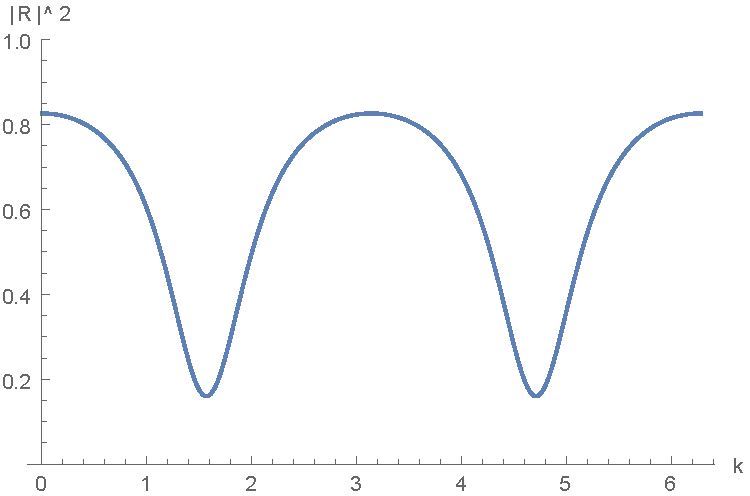
\includegraphics[width=1\textwidth]{img/2gen_reflection_l=1_b1=3_b2=7}
    \caption{$b_1=7, b_2=3$}
  \end{subfigure}
  \begin{subfigure}[t]{0.5\textwidth}
    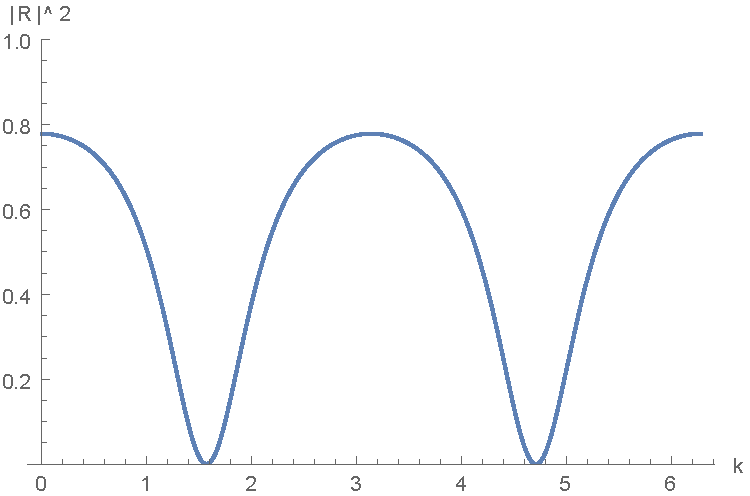
\includegraphics[width=1\textwidth]{img/2gen_reflection_l=1_b1=b2=4}
    \caption{$b_1=b_2=4$}
  \end{subfigure}
  \\
  \begin{subfigure}[t]{0.5\textwidth}
    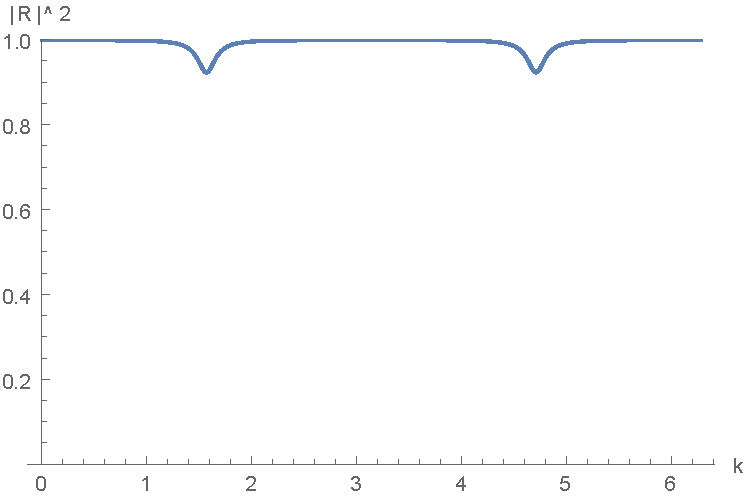
\includegraphics[width=1\textwidth]{img/2gen_reflection_l=1_b1=500_b2=10}
    \caption{$b_1=500, b_2=10$}
  \end{subfigure}
  \begin{subfigure}[t]{0.5\textwidth}
    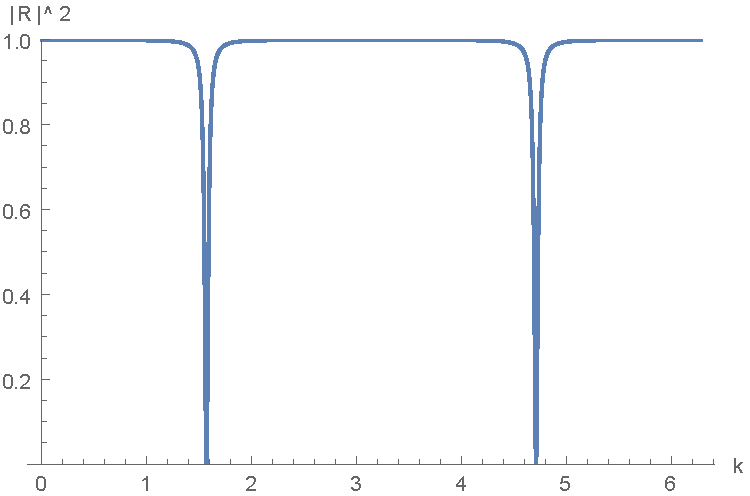
\includegraphics[width=1\textwidth]{img/2gen_reflection_l=1_b1=100_b2=100}
    \caption{$b_1=b_2=100$}
    \label{fig: 2 gen reflection gap}
  \end{subfigure}
  \caption{Reflection $\abs{R}^2$ from 2 generation radial quantum tree graph with inner edge length $\ell_1=1$ and varying branching numbers $b_1$ and $b_2$.}
  \label{fig: 2 gen reflection}
\end{figure}

Let us now consider what happens in the limiting case when one branching number grows large. As we have seen, $b_1$ and $b_2$ occurs symmetrically in the expression for $\abs{R}^2$. Hence we can without loss of generality keep $b_1$ fixed and let $b_2 \to \infty$, then from \eqref{eq: 2 gen reflection probability minimum} we see that the minimal reflection approaces 1, and thus $\abs{R} \to 1$ for all $k$. Similar to the case of the one generation radial quantum tree graph, we have the somewhat counterintuitive result that the probability of getting a reflection increases when the wave has more edges to propagate through. Keep in mind, though, that for $b_1 = b_2$ we always get zero reflection at the points $k = (2n+1)\pi/\ell_1, n = 1,2,3,\ldots$, but the interval for low reflection around these points gets smaller with increasing branching numbers, cf.\ figure~\ref{fig: 2 gen reflection gap}.

To continue this process for an arbitrary number $n$ of generations is unwieldy because one needs to calculate the determinant of a $2n \times 2n$ matrix. Instead, we will in the following chapter develop another method which makes the problem more tractable, and furthermore also gives a better insight into the scattering inside the graph.



% \section{Reflection from radial graphs with $n$ generations}

% General solutions to $Lu=u$ are
% \begin{equation}
%   \psi_j(x) = T_je^{ikx}+R_je^{-ikx}
% \end{equation}
% where $0\leq j\leq n$ is the generation number and $T_0=1, R_n=0$. The standard matching conditions give the system of equations
% \begin{equation}
%   \begin{dcases}
%     \psi_{j-1}(t_j) = \psi_j(t_j) \\
%     -\frac{d}{dx}\psi_{j-1}(t_j) + b_j\frac{d}{dx}\psi_j(t_j) = 0
%   \end{dcases}
%   \quad 1\leq j\leq n
% \end{equation}
% That is
% \begin{equation}
%   \begin{aligned}
%     % j=1: & \begin{cases}
%     %   e^{ikt_j} + R_{j-1} e^{-ikt_j} = T_j e^{ikt_j} + R_j e^{-ikt_j} \\
%     %   -ik(e^{ikt_j} - R_{j-1} e^{-ikt_j}) + b_j ik (T_j e^{ikt_j} - R_j e^{-ikt_j}) = 0
%     % \end{cases}\\
%     % 2\leq j\leq n-1: &
%     \begin{cases}
%       T_{j-1} e^{ikt_j} + R_{j-1} e^{-ikt_j} = T_j e^{ikt_j} + R_j e^{-ikt_j} \\
%       -ik(T_{j-1} e^{ikt_j} - R_{j-1} e^{-ikt_j}) + b_j ik (T_j e^{ikt_j} - R_j e^{-ikt_j}) = 0
%     \end{cases} \\
%     % j=n: & \begin{cases}
%     %   T_{j-1} e^{ikt_j} + R_{j-1} e^{-ikt_j} = T_j e^{ikt_j} \\
%     %   -ik(T_{j-1} e^{ikt_j} - R_{j-1} e^{-ikt_j}) + b_j ik T_j e^{ikt_j} = 0.
%     % \end{cases}
%   \end{aligned}
% \end{equation}
% As a matrix equation for 3 generations
% \begin{equation}
%   \begin{pmatrix}
%     -e^{-ikt_0}  & e^{ikt_0}      & e^{-ikt_0}       & 0              & 0                & 0             \\
%     ike^{-ikt_0} & b_0ike^{ikt_0} & -b_0ike^{-ikt_0} & 0              & 0                & 0             \\
%     0            & -e^{ikt_1}     & -e^{-ikt_1}      & e^{ikt_1}      & e^{-ikt_1}       & 0             \\
%     0            & -ike^{ikt_1}   & ike^{-ikt_1}     & b_1ike^{ikt_1} & -b_1ike^{-ikt_1} & 0             \\
%     0            & 0              & 0                & -e^{ikt_2}     & e^{ikt_2}        & e^{-ikt_2}    \\
%     0            & 0              & 0                & -e^{ikt_2}     & -b_2e^{ikt_2}    & b_2e^{-ikt_2} \\
%   \end{pmatrix}
%   \begin{pmatrix}
%     R \\ A \\ B \\ T_2 \\ R_2 \\ T
%   \end{pmatrix}
%   =
%   \begin{pmatrix}
%     e^{ikt_0} \\ ike^{ikt_0} \\ 0 \\ 0 \\ 0 \\ 0
%   \end{pmatrix}.
% \end{equation}


% Some observations

% \begin{itemize}
%   \item For 3 generations with equal edge lengths $\ell$ and equal branching numbers $m$ we get zero reflection iff
%   \begin{equation}
%     \cos 2k\ell = -\frac{1+m^2}{(1+m)^2}
%   \end{equation}
%   \item For any number of generations with equal length and branching number it appears to always be possible to get zero reflection.
%   \item With $m=2$ and 3 generations, zero reflection is given by at least $\ell_1=2\ell_2$ and $\ell_1=7\ell_2$, and symmetric between $\ell_1$ and $\ell_2$.
%   \item For 3 generations with equal branching number, $|R|^2$ is symmetric between the lengths.
% \end{itemize}


% \section{Minimal average reflection}


\clearpage

\chapter{The snowflake graph}\label{sec: snowflake}
\documentclass[a4paper,11pt]{report}

\usepackage[utf8]{inputenc}
\usepackage[T1]{fontenc}
\usepackage[hidelinks]{hyperref}
\usepackage[nottoc]{tocbibind}
\usepackage{caption}
\usepackage[labelformat=simple]{subcaption}
\renewcommand\thesubfigure{(\alph{subfigure})}

\usepackage{titlesec}

\usepackage{fancyhdr}


% Make section text look nice in header.
% (Only needed for article, not report.)
\makeatletter
\newcommand{\rightorleftmark}{%
  \begingroup\protected@edef\x{\rightmark}%
  \ifx\x\@empty
    \endgroup\leftmark
  \else
    \endgroup\rightmark
  \fi}
\makeatother

% hline in the footer, just like header.
\renewcommand{\footrulewidth}{0.4pt}

\pagestyle{fancy}
\renewcommand{\sectionmark}[1]{\markboth{\thesection~~~{#1}}{}}
\fancyhf{}
\lhead{\textsl{\rightorleftmark}}
\rhead{\thepage}
\lfoot{\textsc{Quantum Snowflake}}
\rfoot{\textsl{Viktor Qvarfordt}}
% \fancypagestyle{plain}{%
%   \fancyhf{}%
%   \renewcommand{\headrulewidth}{0pt}%
% }

\usepackage{mathtools,amssymb,amsthm,enumerate,cleveref}

\usepackage{tikz,tikzscale}
\usetikzlibrary{calc}

% Set up thm, def, etc.
\theoremstyle{plain}
\newtheorem{theorem}{Theorem}[chapter]
\newtheorem{proposition}[theorem]{Proposition}
\newtheorem{lemma}[theorem]{Lemma}
\newtheorem{corollary}[theorem]{Corollary}

\theoremstyle{definition}
\newtheorem{definition}{Definition}[chapter]
% \declaretheorem[name=Example,]{Ex}
\newtheorem{example}{Example}[chapter]
\AtEndEnvironment{example}{\hspace*{0pt}\hfill\ensuremath{\diamondsuit}}

\theoremstyle{remark}
\newtheorem{remark}{Remark}[chapter]

\numberwithin{equation}{chapter}

% \usepackage{showlabels}

\newcommand{\exclude}[1]{}

%% custom commands
\newcommand{\Dom}{\operatorname{Dom}}
\newcommand{\Ran}{\operatorname{Ran}}
\newcommand{\Ker}{\operatorname{Ker}}
\newcommand{\Tr}{\operatorname{Tr}}
\newcommand{\norm}[1]{\left\lVert#1\right\rVert}
\newcommand{\Norm}[1]{\lVert#1\rVert}
\newcommand{\abs}[1]{\left\lvert#1\right\rvert}
\newcommand{\ip}[2]{\ensuremath{\langle #1, #2 \rangle}}

\newcommand{\Z}{\mathbb{Z}}
\newcommand{\R}{\mathbb{R}}
\newcommand{\C}{\mathbb{C}}
\renewcommand{\H}{\mathcal{H}}

\newcommand{\D}[2]{\frac{d#1}{d#2}}
\newcommand{\pD}[2]{\frac{\partial#1}{\partial#2}}

\newcommand{\Dn}[3]{\frac{d^#3#1}{d#2^#3}}
\newcommand{\pDn}[3]{\frac{\partial^#3#1}{\partial#2^#3}}

\newcommand{\Dop}[1]{\frac{d}{d#1}}
\newcommand{\pDop}[1]{\frac{\partial}{\partial#1}}

\newcommand{\Dopn}[2]{\frac{d^#2}{d#1^#2}}
\newcommand{\pDopn}[2]{\frac{\partial^#2}{\partial#1^#2}}


\newcommand{\g}[1]{\left(#1\right)}


\title{Quantum Snowflake}
\author{Viktor Qvarfordt}


\begin{document}

\begin{titlepage}
  \thispagestyle{empty}
  % \null\vskip{-2em}
  % \noindent \large{\textbf{Stockholm University \hfill Fysikum}}
  % \vskip 7em
  \centering
  \null
  \vspace{3cm}
  {\huge\bf Quantum Snowflake} \\
  \vspace{1cm}
  {\Large\sl Viktor Qvarfordt} \\
  \vspace{0.5cm}
  {\Large May 2015} \\
  \vspace{4cm}
  {\Large Bachelor’s Thesis --- 15 ECTS} \\
  \vspace{0.5cm}
  \Large
  Supervisor: Pavel Kurasov \\
  \vspace{5cm}
  Department of Mathematics, Department of Physics \\
  \vspace{0.5cm}
  Stockholm University \\
  \vfill
  {\tiny Revised \today}
  \vspace{-1cm}
\end{titlepage}

\begin{abstract}
  \input{content/abstract}
\end{abstract}
% \thispagestyle{empty}
\clearpage

% \renewcommand{\abstractname}{Acknowledgments}
% \begin{abstract}
%   \input{content/acknowledgments}
% \end{abstract}
% \thispagestyle{empty}
% \newpage

% \begin{figure}
%   \centering
%   \includegraphics[angle=90,width=\textwidth]{img/{snowflake_4_0.35_7_4_0.5}.pdf}
% \end{figure}

\fancypagestyle{snowflake}{\lhead{\textsl{Illustration of a quantum snowflake}}}
\thispagestyle{snowflake}
\setcounter{page}{3}
\begin{figure}
  \centering
  \includegraphics[width=\textwidth]{img/{snowflake_2_0.6_13_4_0.8}.pdf}
\end{figure}

\clearpage

{
\titleformat{\chapter}[display]{\normalfont\huge\bfseries}{\chaptertitlename~\thechapter}{20pt}{\Huge}
\titlespacing*{\chapter}{0pt}{-50pt}{25pt}
\tableofcontents
\clearpage
}

\chapter{Introduction}\label{sec: physical interpretation}\label{sec: introduction}
\input{content/introduction}
\clearpage

\fancypagestyle{automatic}{\lhead{\textsl{\rightorleftmark}}}
\pagestyle{automatic}

\chapter{Defining quantum graphs}\label{sec: defining quantum graphs}
\input{content/quantum_graphs}
\clearpage

\chapter{Properties of quantum graphs}\label{sec: properties}
\input{content/properties_of_quantum_graphs}
\clearpage

\chapter{The snowflake graph}\label{sec: snowflake}
\input{content/snowflake}
\clearpage

\fancypagestyle{conclusion}{\lhead{\textsl{Conclusion}}}
\pagestyle{conclusion}
\chapter{Conclusion}\label{sec: conclusion}
\input{content/conclusion}
\clearpage

\thispagestyle{snowflake}
\begin{figure}
  \centering
  \includegraphics[angle=90,width=\textwidth]{img/{snowflake_4_0.35_7_4_0.5}.pdf}
\end{figure}

\fancypagestyle{bibliography}{\lhead{\textsl{Bibliography}}}
\pagestyle{bibliography}
\input{content/bibliography}

\end{document}

\clearpage

\fancypagestyle{conclusion}{\lhead{\textsl{Conclusion}}}
\pagestyle{conclusion}
\chapter{Conclusion}\label{sec: conclusion}
In \cref{sec: introduction} we gave a broad background to the physics that underpin the motivation for studying quantum graphs. In \cref{sec: defining quantum graphs} we defined quantum graphs and discussed the three components: metric graphs, differential operators and matching conditions. In \cref{sec: properties} we studied various properties of quantum graphs that formed the basis for \cref{sec: snowflake}, including scattering phenomena, exploitation of graph symmetries and the introduction of radial quantum tree graphs as generalizations of star graphs.

Scattering properties of radial quantum tree graphs with two generations where studied via a direct method of calculating the scattering amplitude, found to be given by
\[
  R_2(k) = -\frac{(b_1-1) (b_2+1)+(b_1+1) (b_2-1) e^{2 i k \ell}}{(b_1+1) (b_2+1)+(b_1-1) (b_2-1) e^{2 i k \ell}}
\]
for an incoming wave with energy $\lambda = k^2$.
Already for this simple graph interesting results where found: The above expression is invariant when interchanging the branching numbers $b_1$ and $b_2$, showing that the corresponding two different graphs exhibit identical scattering properties and can thus not be distinguished by external measurements of the graph.

The simple method of calculating the reflection amplitude proved to be limited when generalizing to radial graphs of higher number of generations. For this reason the snowflake graph was introduced as the central object of study in \cref{sec: snowflake}.

The quantum snowflake is defined as a radial quantum tree graph with infinite number of generations, where all branching numbers equal $m$, and the length of edges in generation $n$ are given by $\ell\beta^n$ for constants $\ell$ and $\beta$. By construction the snowflake graph exhibits self-similarity and has a finite depth $\ell/(1-\beta)$ if $\beta < 1$.

By exploiting the rotational symmetry and self-similarity of the snowflake graph, we decomposed every eigenfunction $f$ to the Laplace operator $L=-\Dopn{x}{2}$ on the graph into $m$ quasi rotation invariant components
\[
  f^n_j = \frac{1}{m} \sum_{k=0}^{m-1} z^{-nk} f_{j+1}, \quad j=1,2,\ldots,m.
\]
$f_j$ denotes the restriction of $f$ to the $j$:th edge and $z=e^{\frac{2\pi}{m}i}$ is the first eigenvalue to the rotation operator $R: e_j \mapsto e_{j+1}$.
The functions $f^n_j$ are eigenfunctions to the rotation operator $R$ and sum to $f_j = \sum_{n=0}^{m-1} f_j^n$.

Based on this decomposition of eigenfunctions on the snowflake graph $\Gamma$ we developed a  method for transforming $\Gamma$ with standard matching conditions into a line graph $\widetilde{\Gamma}$ with snowflake matching conditions. At vertex $v$ we have the conditions
\begin{align*}
  \!\begin{array}{c}
    \Gamma \\
    \text{standard} \\
    \text{conditions}
  \end{array}\!\!\!:
  \begin{dcases}
    f(x) = f(y) \quad \forall x \in v \\
    \sum_{x\in v}  \partial f(x) = 0
  \end{dcases}
  &&
  \!\!\!\!\begin{array}{c}
    \widetilde{\Gamma} \\
    \text{snowflake} \\
    \text{conditions}
  \end{array}\!\!\!:
  \begin{dcases}
    f_0(v) = \frac{1}{\sqrt{m}} f_1(v) \\
    \partial f_0(v) + \sqrt{m} \partial f_1(v) = 0.
  \end{dcases}
\end{align*}
Under these conditions the two graphs $\Gamma$ and $\widetilde{\Gamma}$ have identical scattering properties, allowing us to consider only the simpler graph $\widetilde{\Gamma}$.

For $\widetilde{\Gamma}$ we developed a method for combining several vertices into one vertex, which allowed us characterize the internal scattering of the snowflake graph. From this the total reflection $R_n(k) = S_{ll,n}(k)$ of a snowflake graph with $n$ generations was found to be given recursively by
\begin{align*}
  \left\lbrace\!
  \begin{aligned}
    S_{ll,1} &= \frac{1-m}{1+m} \\
    S_{rl,1} &= \frac{2\sqrt{m}}{1+m} \\
    S_{rr,1} &= -S_{ll,1} \\
    S_{lr,1} &= S_{rl,1}
  \end{aligned}\right.
  &&
  \left\lbrace\!
  \begin{aligned}
    S_{ll,n+1} &= S_{ll,n} + \frac{e^{2ik\ell_n} S_{rl,n} S_{ll,1} S_{lr,n}}{1 - e^{2ik\ell_n} S_{rr,n} S_{ll,1}} \\
    S_{rl,n+1} &= \frac{e^{ik\ell_n} S_{rl,n} S_{rl,1}}{1 - e^{2ik\ell_n} S_{ll,1} S_{rr,n}} \\
    S_{rr,n+1} &= S_{rr,1} + \frac{e^{2ik\ell_n} S_{lr,1} S_{rr,n} S_{rl,1}}{1 - e^{2ik\ell_n} S_{ll,1} S_{rr,n}} \\
    S_{lr,n+1} &= \frac{e^{ik\ell_n} S_{lr,1}S_{lr,n}}{1 - e^{2ik\ell_n} S_{rr,n} S_{ll,1}}
  \end{aligned}\right.
\end{align*}
where $S_{ij_n}, i,j=r,l$ denotes the transition amplitude from $j$ to $i$ for a combined vertex consisting of $n$ ordinary vertices.

This allowed us to formulate several results: For any snowflake graph with $n$ generations and branching number $m$, the reflection of an incoming wave with zero energy is given by
\[
  S_{ll,n}(0) = \frac{1-m^n}{1+m^n} = \frac{2}{m^n+1} - 1,
\]
precisely that of a star graph with degree $m^n+1$. That is, for very low energies the incoming wave does not ``see'' the inner edges.

We also found that if the branching number $m$ increases, then also the reflection probability $\abs{S_{ll,n}(k)}^2$ increases, except for the case when it is 0 or~1.

Furthermore we showed that the the periodic snowflake graph, i.e.\ with $\beta=1$, behaves as a crystalline material and admits a periodic band gap structure. If the periodic snowflake graph has edge lengths $\ell$ and branching number $m$, then only energies $\lambda = k^2$ satisfying
\[
  \abs{\cos k\ell} < \frac{2\sqrt{m}}{m+1}
\]
are realizable in the graph. Incoming waves with energies not satisfying this inequality are totally reflected.

However, a complete characterization of the reflection amplitude $R(k) = \lim_{n\to\infty} S_{ll,n}$ for arbitrary $0<\beta<1$ could no be found. In general $R(k)$ is not periodic and appears to vary very irregularly with $k$.

Although the recursive expression for $R_n$ in principle determines the reflection amplitude in the general case, it is very difficult to work with. Improvements can be made to the method of combining vertices, the fact that the graph is self-similar is currently not being used. The ambition should be to find a closed form expression for $R_{n,m,\beta}(k)$.

Furthermore it would be interesting to study the average reflection
\[
  \frac{1}{k_1} \int_{0}^{k_1} R(k) \, dk.
\]
From a physical or practical point of view this particularly interesting: It is generally not possible to have precise control of the energy of the wave that is sent to the graph, most often one has waves from a range of energies. The numerically calculated result
\[
  \frac{1}{2\pi\ell} \int_{0}^{2\pi\ell} \abs{R(k)}^2 dk = \frac{m-1}{m+1} = \abs{R_1(0)}
\]
for $n\to\infty$, $\beta=1$ and branching number $m$, indicates that strong regularity can be found for the average reflection.

\clearpage

\thispagestyle{snowflake}
\begin{figure}
  \centering
  \includegraphics[angle=90,width=\textwidth]{img/{snowflake_4_0.35_7_4_0.5}.pdf}
\end{figure}

\fancypagestyle{bibliography}{\lhead{\textsl{Bibliography}}}
\pagestyle{bibliography}
\begin{thebibliography}{99}

  \bibitem{pavel book}
  Pavel Kurasov,
  \textit{Quantum graphs: Spectral theory and inverse problems},
  To be published

  \bibitem{symmetries boman kurasov}
  Jan Boman, Pavel Kurasov,
  \textit{Symmetries of quantum graphs and the inverse scattering problem},
  Advances in Applied Mathematics 35 (2005) 58-70

  \bibitem{introduction and brief survey}
  Peter Kuchment,
  \textit{Quantum graphs: an introduction and a brief survey},
  \texttt{arXiv:0802.3442}

  \bibitem{berkolaiko kuchment book}
  Gregory Berkolaiko, Peter Kuchment,
  \textit{Introduction to Quantum Graphs},
  AMS 2013

  \bibitem{schmudgen}
  Konrad Schmüdgen,
  \textit{Unbounded Self-adjoint Operators on Hilbert Space},
  Springer 2012

  \bibitem{pedersen}
  Gert K. Pedersen,
  \textit{Analysis Now},
  Springer 1989

  \bibitem{teschl-fa}
  Gerald Teschl,
  \textit{Topics in Real and Functional Analysis},
  \url{http://www.mat.univie.ac.at/~gerald/ftp/book-fa/fa.pdf} 2015

  \bibitem{teschl-schroe}
  Gerald Teschl,
  \textit{Mathematical Methods in Quantum Mechanics: With applications to Schrödinger operators},
  AMS 2009

  \bibitem{friedman}
  Avner Friedman,
  \textit{Foundations of modern analysis},
  Dover Publications, 1982

  \bibitem{adams sobolev spaces}
  Robert A. Adams,
  \textit{Sobolev Spaces},
  Academic Press, 1975

  \bibitem{ballentine}
  Leslie E. Ballentine,
  \textit{Quantum Mechanics: A modern development},
  World Scientific Publishing 1998

  \bibitem{}
  Peter D. Hislop, Olaf Post,
  \textit{Anderson Localization for radial tree-like random quantum graphs},
  \texttt{arXiv:math-ph/0611022} 2008

  \bibitem{SE derivaiton}
  David W. Ward, Sabine Volkmer,
  \textit{How to Derive the Schrödinger Equation},
  \texttt{arXiv:physics/0610121}

  \bibitem{lax}
  Peter D. Lax,
  \textit{Functional analysis},
  John Wiley \& Sons, Inc. 2002

  \bibitem{born statistical interpretation}
  Max Born,
  \textit{On the quantum mechanics of collisions},
  \url{http://hermes.ffn.ub.es/luisnavarro/nuevo_maletin/Born_1926_statistical_interpretation.pdf}

  \bibitem{vaidman mwi}
  Lev Vaidman,
  \textit{On schizophrenic experiences of the neutron or why we should believe in the many-worlds interpretation of quantum theory}
  \url{http://xxx.lanl.gov/pdf/quant-ph/9609006.pdf}

  \bibitem{carroll EQM probability}
  Charles T. Sebens and Sean M. Carroll,
  \textit{Self-Locating Uncertainty and the Origin of Probability in Everettian Quantum Mechanics},
  \texttt{arXiv:1405.7577}

  \bibitem{wallace born rule}
  David Wallace,
  \textit{A formal proof of the Born rule from decision-theoretic assumptions},
  \texttt{arXiv:0906.2718}

  \bibitem{tegmark}
  Max Tegmark,
  \textit{The Mathematical Universe},
  \texttt{arXiv:0704.0646}

  \bibitem{qbism and the greeks}
  Christopher A. Fuchs and Rüdiger Schack,
  \textit{QBism and the Greeks: why a quantum state does not represent an element of physical reality},
  \texttt{arXiv:1412.4211}

  \bibitem{qbism introduction}
  Christopher A. Fuchs, N. David Mermin and Rüdiger Schack,
  \textit{An Introduction to QBism with an Application to the Locality of Quantum Mechanics},
  \texttt{arXiv:1311.5253}

  \bibitem{feynman quantum mechanics}
  Richard P. Feynman,
  \textit{Space-Time Approach to Non-Relativistic Quantum Mechanics},
  \url{http://web.ihep.su/dbserv/compas/src/feynman48c/eng.pdf}


\end{thebibliography}


\end{document}

\clearpage

\fancypagestyle{conclusion}{\lhead{\textsl{Conclusion}}}
\pagestyle{conclusion}
\chapter{Conclusion}\label{sec: conclusion}
In \cref{sec: introduction} we gave a broad background to the physics that underpin the motivation for studying quantum graphs. In \cref{sec: defining quantum graphs} we defined quantum graphs and discussed the three components: metric graphs, differential operators and matching conditions. In \cref{sec: properties} we studied various properties of quantum graphs that formed the basis for \cref{sec: snowflake}, including scattering phenomena, exploitation of graph symmetries and the introduction of radial quantum tree graphs as generalizations of star graphs.

Scattering properties of radial quantum tree graphs with two generations where studied via a direct method of calculating the scattering amplitude, found to be given by
\[
  R_2(k) = -\frac{(b_1-1) (b_2+1)+(b_1+1) (b_2-1) e^{2 i k \ell}}{(b_1+1) (b_2+1)+(b_1-1) (b_2-1) e^{2 i k \ell}}
\]
for an incoming wave with energy $\lambda = k^2$.
Already for this simple graph interesting results where found: The above expression is invariant when interchanging the branching numbers $b_1$ and $b_2$, showing that the corresponding two different graphs exhibit identical scattering properties and can thus not be distinguished by external measurements of the graph.

The simple method of calculating the reflection amplitude proved to be limited when generalizing to radial graphs of higher number of generations. For this reason the snowflake graph was introduced as the central object of study in \cref{sec: snowflake}.

The quantum snowflake is defined as a radial quantum tree graph with infinite number of generations, where all branching numbers equal $m$, and the length of edges in generation $n$ are given by $\ell\beta^n$ for constants $\ell$ and $\beta$. By construction the snowflake graph exhibits self-similarity and has a finite depth $\ell/(1-\beta)$ if $\beta < 1$.

By exploiting the rotational symmetry and self-similarity of the snowflake graph, we decomposed every eigenfunction $f$ to the Laplace operator $L=-\Dopn{x}{2}$ on the graph into $m$ quasi rotation invariant components
\[
  f^n_j = \frac{1}{m} \sum_{k=0}^{m-1} z^{-nk} f_{j+1}, \quad j=1,2,\ldots,m.
\]
$f_j$ denotes the restriction of $f$ to the $j$:th edge and $z=e^{\frac{2\pi}{m}i}$ is the first eigenvalue to the rotation operator $R: e_j \mapsto e_{j+1}$.
The functions $f^n_j$ are eigenfunctions to the rotation operator $R$ and sum to $f_j = \sum_{n=0}^{m-1} f_j^n$.

Based on this decomposition of eigenfunctions on the snowflake graph $\Gamma$ we developed a  method for transforming $\Gamma$ with standard matching conditions into a line graph $\widetilde{\Gamma}$ with snowflake matching conditions. At vertex $v$ we have the conditions
\begin{align*}
  \!\begin{array}{c}
    \Gamma \\
    \text{standard} \\
    \text{conditions}
  \end{array}\!\!\!:
  \begin{dcases}
    f(x) = f(y) \quad \forall x \in v \\
    \sum_{x\in v}  \partial f(x) = 0
  \end{dcases}
  &&
  \!\!\!\!\begin{array}{c}
    \widetilde{\Gamma} \\
    \text{snowflake} \\
    \text{conditions}
  \end{array}\!\!\!:
  \begin{dcases}
    f_0(v) = \frac{1}{\sqrt{m}} f_1(v) \\
    \partial f_0(v) + \sqrt{m} \partial f_1(v) = 0.
  \end{dcases}
\end{align*}
Under these conditions the two graphs $\Gamma$ and $\widetilde{\Gamma}$ have identical scattering properties, allowing us to consider only the simpler graph $\widetilde{\Gamma}$.

For $\widetilde{\Gamma}$ we developed a method for combining several vertices into one vertex, which allowed us characterize the internal scattering of the snowflake graph. From this the total reflection $R_n(k) = S_{ll,n}(k)$ of a snowflake graph with $n$ generations was found to be given recursively by
\begin{align*}
  \left\lbrace\!
  \begin{aligned}
    S_{ll,1} &= \frac{1-m}{1+m} \\
    S_{rl,1} &= \frac{2\sqrt{m}}{1+m} \\
    S_{rr,1} &= -S_{ll,1} \\
    S_{lr,1} &= S_{rl,1}
  \end{aligned}\right.
  &&
  \left\lbrace\!
  \begin{aligned}
    S_{ll,n+1} &= S_{ll,n} + \frac{e^{2ik\ell_n} S_{rl,n} S_{ll,1} S_{lr,n}}{1 - e^{2ik\ell_n} S_{rr,n} S_{ll,1}} \\
    S_{rl,n+1} &= \frac{e^{ik\ell_n} S_{rl,n} S_{rl,1}}{1 - e^{2ik\ell_n} S_{ll,1} S_{rr,n}} \\
    S_{rr,n+1} &= S_{rr,1} + \frac{e^{2ik\ell_n} S_{lr,1} S_{rr,n} S_{rl,1}}{1 - e^{2ik\ell_n} S_{ll,1} S_{rr,n}} \\
    S_{lr,n+1} &= \frac{e^{ik\ell_n} S_{lr,1}S_{lr,n}}{1 - e^{2ik\ell_n} S_{rr,n} S_{ll,1}}
  \end{aligned}\right.
\end{align*}
where $S_{ij_n}, i,j=r,l$ denotes the transition amplitude from $j$ to $i$ for a combined vertex consisting of $n$ ordinary vertices.

This allowed us to formulate several results: For any snowflake graph with $n$ generations and branching number $m$, the reflection of an incoming wave with zero energy is given by
\[
  S_{ll,n}(0) = \frac{1-m^n}{1+m^n} = \frac{2}{m^n+1} - 1,
\]
precisely that of a star graph with degree $m^n+1$. That is, for very low energies the incoming wave does not ``see'' the inner edges.

We also found that if the branching number $m$ increases, then also the reflection probability $\abs{S_{ll,n}(k)}^2$ increases, except for the case when it is 0 or~1.

Furthermore we showed that the the periodic snowflake graph, i.e.\ with $\beta=1$, behaves as a crystalline material and admits a periodic band gap structure. If the periodic snowflake graph has edge lengths $\ell$ and branching number $m$, then only energies $\lambda = k^2$ satisfying
\[
  \abs{\cos k\ell} < \frac{2\sqrt{m}}{m+1}
\]
are realizable in the graph. Incoming waves with energies not satisfying this inequality are totally reflected.

However, a complete characterization of the reflection amplitude $R(k) = \lim_{n\to\infty} S_{ll,n}$ for arbitrary $0<\beta<1$ could no be found. In general $R(k)$ is not periodic and appears to vary very irregularly with $k$.

Although the recursive expression for $R_n$ in principle determines the reflection amplitude in the general case, it is very difficult to work with. Improvements can be made to the method of combining vertices, the fact that the graph is self-similar is currently not being used. The ambition should be to find a closed form expression for $R_{n,m,\beta}(k)$.

Furthermore it would be interesting to study the average reflection
\[
  \frac{1}{k_1} \int_{0}^{k_1} R(k) \, dk.
\]
From a physical or practical point of view this particularly interesting: It is generally not possible to have precise control of the energy of the wave that is sent to the graph, most often one has waves from a range of energies. The numerically calculated result
\[
  \frac{1}{2\pi\ell} \int_{0}^{2\pi\ell} \abs{R(k)}^2 dk = \frac{m-1}{m+1} = \abs{R_1(0)}
\]
for $n\to\infty$, $\beta=1$ and branching number $m$, indicates that strong regularity can be found for the average reflection.

\clearpage

\thispagestyle{snowflake}
\begin{figure}
  \centering
  \includegraphics[angle=90,width=\textwidth]{img/{snowflake_4_0.35_7_4_0.5}.pdf}
\end{figure}

\fancypagestyle{bibliography}{\lhead{\textsl{Bibliography}}}
\pagestyle{bibliography}
\begin{thebibliography}{99}

  \bibitem{pavel book}
  Pavel Kurasov,
  \textit{Quantum graphs: Spectral theory and inverse problems},
  To be published

  \bibitem{symmetries boman kurasov}
  Jan Boman, Pavel Kurasov,
  \textit{Symmetries of quantum graphs and the inverse scattering problem},
  Advances in Applied Mathematics 35 (2005) 58-70

  \bibitem{introduction and brief survey}
  Peter Kuchment,
  \textit{Quantum graphs: an introduction and a brief survey},
  \texttt{arXiv:0802.3442}

  \bibitem{berkolaiko kuchment book}
  Gregory Berkolaiko, Peter Kuchment,
  \textit{Introduction to Quantum Graphs},
  AMS 2013

  \bibitem{schmudgen}
  Konrad Schmüdgen,
  \textit{Unbounded Self-adjoint Operators on Hilbert Space},
  Springer 2012

  \bibitem{pedersen}
  Gert K. Pedersen,
  \textit{Analysis Now},
  Springer 1989

  \bibitem{teschl-fa}
  Gerald Teschl,
  \textit{Topics in Real and Functional Analysis},
  \url{http://www.mat.univie.ac.at/~gerald/ftp/book-fa/fa.pdf} 2015

  \bibitem{teschl-schroe}
  Gerald Teschl,
  \textit{Mathematical Methods in Quantum Mechanics: With applications to Schrödinger operators},
  AMS 2009

  \bibitem{friedman}
  Avner Friedman,
  \textit{Foundations of modern analysis},
  Dover Publications, 1982

  \bibitem{adams sobolev spaces}
  Robert A. Adams,
  \textit{Sobolev Spaces},
  Academic Press, 1975

  \bibitem{ballentine}
  Leslie E. Ballentine,
  \textit{Quantum Mechanics: A modern development},
  World Scientific Publishing 1998

  \bibitem{}
  Peter D. Hislop, Olaf Post,
  \textit{Anderson Localization for radial tree-like random quantum graphs},
  \texttt{arXiv:math-ph/0611022} 2008

  \bibitem{SE derivaiton}
  David W. Ward, Sabine Volkmer,
  \textit{How to Derive the Schrödinger Equation},
  \texttt{arXiv:physics/0610121}

  \bibitem{lax}
  Peter D. Lax,
  \textit{Functional analysis},
  John Wiley \& Sons, Inc. 2002

  \bibitem{born statistical interpretation}
  Max Born,
  \textit{On the quantum mechanics of collisions},
  \url{http://hermes.ffn.ub.es/luisnavarro/nuevo_maletin/Born_1926_statistical_interpretation.pdf}

  \bibitem{vaidman mwi}
  Lev Vaidman,
  \textit{On schizophrenic experiences of the neutron or why we should believe in the many-worlds interpretation of quantum theory}
  \url{http://xxx.lanl.gov/pdf/quant-ph/9609006.pdf}

  \bibitem{carroll EQM probability}
  Charles T. Sebens and Sean M. Carroll,
  \textit{Self-Locating Uncertainty and the Origin of Probability in Everettian Quantum Mechanics},
  \texttt{arXiv:1405.7577}

  \bibitem{wallace born rule}
  David Wallace,
  \textit{A formal proof of the Born rule from decision-theoretic assumptions},
  \texttt{arXiv:0906.2718}

  \bibitem{tegmark}
  Max Tegmark,
  \textit{The Mathematical Universe},
  \texttt{arXiv:0704.0646}

  \bibitem{qbism and the greeks}
  Christopher A. Fuchs and Rüdiger Schack,
  \textit{QBism and the Greeks: why a quantum state does not represent an element of physical reality},
  \texttt{arXiv:1412.4211}

  \bibitem{qbism introduction}
  Christopher A. Fuchs, N. David Mermin and Rüdiger Schack,
  \textit{An Introduction to QBism with an Application to the Locality of Quantum Mechanics},
  \texttt{arXiv:1311.5253}

  \bibitem{feynman quantum mechanics}
  Richard P. Feynman,
  \textit{Space-Time Approach to Non-Relativistic Quantum Mechanics},
  \url{http://web.ihep.su/dbserv/compas/src/feynman48c/eng.pdf}


\end{thebibliography}


\end{document}

\clearpage

\fancypagestyle{conclusion}{\lhead{\textsl{Conclusion}}}
\pagestyle{conclusion}
\chapter{Conclusion}\label{sec: conclusion}
In \cref{sec: introduction} we gave a broad background to the physics that underpin the motivation for studying quantum graphs. In \cref{sec: defining quantum graphs} we defined quantum graphs and discussed the three components: metric graphs, differential operators and matching conditions. In \cref{sec: properties} we studied various properties of quantum graphs that formed the basis for \cref{sec: snowflake}, including scattering phenomena, exploitation of graph symmetries and the introduction of radial quantum tree graphs as generalizations of star graphs.

Scattering properties of radial quantum tree graphs with two generations where studied via a direct method of calculating the scattering amplitude, found to be given by
\[
  R_2(k) = -\frac{(b_1-1) (b_2+1)+(b_1+1) (b_2-1) e^{2 i k \ell}}{(b_1+1) (b_2+1)+(b_1-1) (b_2-1) e^{2 i k \ell}}
\]
for an incoming wave with energy $\lambda = k^2$.
Already for this simple graph interesting results where found: The above expression is invariant when interchanging the branching numbers $b_1$ and $b_2$, showing that the corresponding two different graphs exhibit identical scattering properties and can thus not be distinguished by external measurements of the graph.

The simple method of calculating the reflection amplitude proved to be limited when generalizing to radial graphs of higher number of generations. For this reason the snowflake graph was introduced as the central object of study in \cref{sec: snowflake}.

The quantum snowflake is defined as a radial quantum tree graph with infinite number of generations, where all branching numbers equal $m$, and the length of edges in generation $n$ are given by $\ell\beta^n$ for constants $\ell$ and $\beta$. By construction the snowflake graph exhibits self-similarity and has a finite depth $\ell/(1-\beta)$ if $\beta < 1$.

By exploiting the rotational symmetry and self-similarity of the snowflake graph, we decomposed every eigenfunction $f$ to the Laplace operator $L=-\Dopn{x}{2}$ on the graph into $m$ quasi rotation invariant components
\[
  f^n_j = \frac{1}{m} \sum_{k=0}^{m-1} z^{-nk} f_{j+1}, \quad j=1,2,\ldots,m.
\]
$f_j$ denotes the restriction of $f$ to the $j$:th edge and $z=e^{\frac{2\pi}{m}i}$ is the first eigenvalue to the rotation operator $R: e_j \mapsto e_{j+1}$.
The functions $f^n_j$ are eigenfunctions to the rotation operator $R$ and sum to $f_j = \sum_{n=0}^{m-1} f_j^n$.

Based on this decomposition of eigenfunctions on the snowflake graph $\Gamma$ we developed a  method for transforming $\Gamma$ with standard matching conditions into a line graph $\widetilde{\Gamma}$ with snowflake matching conditions. At vertex $v$ we have the conditions
\begin{align*}
  \!\begin{array}{c}
    \Gamma \\
    \text{standard} \\
    \text{conditions}
  \end{array}\!\!\!:
  \begin{dcases}
    f(x) = f(y) \quad \forall x \in v \\
    \sum_{x\in v}  \partial f(x) = 0
  \end{dcases}
  &&
  \!\!\!\!\begin{array}{c}
    \widetilde{\Gamma} \\
    \text{snowflake} \\
    \text{conditions}
  \end{array}\!\!\!:
  \begin{dcases}
    f_0(v) = \frac{1}{\sqrt{m}} f_1(v) \\
    \partial f_0(v) + \sqrt{m} \partial f_1(v) = 0.
  \end{dcases}
\end{align*}
Under these conditions the two graphs $\Gamma$ and $\widetilde{\Gamma}$ have identical scattering properties, allowing us to consider only the simpler graph $\widetilde{\Gamma}$.

For $\widetilde{\Gamma}$ we developed a method for combining several vertices into one vertex, which allowed us characterize the internal scattering of the snowflake graph. From this the total reflection $R_n(k) = S_{ll,n}(k)$ of a snowflake graph with $n$ generations was found to be given recursively by
\begin{align*}
  \left\lbrace\!
  \begin{aligned}
    S_{ll,1} &= \frac{1-m}{1+m} \\
    S_{rl,1} &= \frac{2\sqrt{m}}{1+m} \\
    S_{rr,1} &= -S_{ll,1} \\
    S_{lr,1} &= S_{rl,1}
  \end{aligned}\right.
  &&
  \left\lbrace\!
  \begin{aligned}
    S_{ll,n+1} &= S_{ll,n} + \frac{e^{2ik\ell_n} S_{rl,n} S_{ll,1} S_{lr,n}}{1 - e^{2ik\ell_n} S_{rr,n} S_{ll,1}} \\
    S_{rl,n+1} &= \frac{e^{ik\ell_n} S_{rl,n} S_{rl,1}}{1 - e^{2ik\ell_n} S_{ll,1} S_{rr,n}} \\
    S_{rr,n+1} &= S_{rr,1} + \frac{e^{2ik\ell_n} S_{lr,1} S_{rr,n} S_{rl,1}}{1 - e^{2ik\ell_n} S_{ll,1} S_{rr,n}} \\
    S_{lr,n+1} &= \frac{e^{ik\ell_n} S_{lr,1}S_{lr,n}}{1 - e^{2ik\ell_n} S_{rr,n} S_{ll,1}}
  \end{aligned}\right.
\end{align*}
where $S_{ij_n}, i,j=r,l$ denotes the transition amplitude from $j$ to $i$ for a combined vertex consisting of $n$ ordinary vertices.

This allowed us to formulate several results: For any snowflake graph with $n$ generations and branching number $m$, the reflection of an incoming wave with zero energy is given by
\[
  S_{ll,n}(0) = \frac{1-m^n}{1+m^n} = \frac{2}{m^n+1} - 1,
\]
precisely that of a star graph with degree $m^n+1$. That is, for very low energies the incoming wave does not ``see'' the inner edges.

We also found that if the branching number $m$ increases, then also the reflection probability $\abs{S_{ll,n}(k)}^2$ increases, except for the case when it is 0 or~1.

Furthermore we showed that the the periodic snowflake graph, i.e.\ with $\beta=1$, behaves as a crystalline material and admits a periodic band gap structure. If the periodic snowflake graph has edge lengths $\ell$ and branching number $m$, then only energies $\lambda = k^2$ satisfying
\[
  \abs{\cos k\ell} < \frac{2\sqrt{m}}{m+1}
\]
are realizable in the graph. Incoming waves with energies not satisfying this inequality are totally reflected.

However, a complete characterization of the reflection amplitude $R(k) = \lim_{n\to\infty} S_{ll,n}$ for arbitrary $0<\beta<1$ could no be found. In general $R(k)$ is not periodic and appears to vary very irregularly with $k$.

Although the recursive expression for $R_n$ in principle determines the reflection amplitude in the general case, it is very difficult to work with. Improvements can be made to the method of combining vertices, the fact that the graph is self-similar is currently not being used. The ambition should be to find a closed form expression for $R_{n,m,\beta}(k)$.

Furthermore it would be interesting to study the average reflection
\[
  \frac{1}{k_1} \int_{0}^{k_1} R(k) \, dk.
\]
From a physical or practical point of view this particularly interesting: It is generally not possible to have precise control of the energy of the wave that is sent to the graph, most often one has waves from a range of energies. The numerically calculated result
\[
  \frac{1}{2\pi\ell} \int_{0}^{2\pi\ell} \abs{R(k)}^2 dk = \frac{m-1}{m+1} = \abs{R_1(0)}
\]
for $n\to\infty$, $\beta=1$ and branching number $m$, indicates that strong regularity can be found for the average reflection.

\clearpage

\thispagestyle{snowflake}
\begin{figure}
  \centering
  \includegraphics[angle=90,width=\textwidth]{img/{snowflake_4_0.35_7_4_0.5}.pdf}
\end{figure}

\fancypagestyle{bibliography}{\lhead{\textsl{Bibliography}}}
\pagestyle{bibliography}
\begin{thebibliography}{99}

  \bibitem{pavel book}
  Pavel Kurasov,
  \textit{Quantum graphs: Spectral theory and inverse problems},
  To be published

  \bibitem{symmetries boman kurasov}
  Jan Boman, Pavel Kurasov,
  \textit{Symmetries of quantum graphs and the inverse scattering problem},
  Advances in Applied Mathematics 35 (2005) 58-70

  \bibitem{introduction and brief survey}
  Peter Kuchment,
  \textit{Quantum graphs: an introduction and a brief survey},
  \texttt{arXiv:0802.3442}

  \bibitem{berkolaiko kuchment book}
  Gregory Berkolaiko, Peter Kuchment,
  \textit{Introduction to Quantum Graphs},
  AMS 2013

  \bibitem{schmudgen}
  Konrad Schmüdgen,
  \textit{Unbounded Self-adjoint Operators on Hilbert Space},
  Springer 2012

  \bibitem{pedersen}
  Gert K. Pedersen,
  \textit{Analysis Now},
  Springer 1989

  \bibitem{teschl-fa}
  Gerald Teschl,
  \textit{Topics in Real and Functional Analysis},
  \url{http://www.mat.univie.ac.at/~gerald/ftp/book-fa/fa.pdf} 2015

  \bibitem{teschl-schroe}
  Gerald Teschl,
  \textit{Mathematical Methods in Quantum Mechanics: With applications to Schrödinger operators},
  AMS 2009

  \bibitem{friedman}
  Avner Friedman,
  \textit{Foundations of modern analysis},
  Dover Publications, 1982

  \bibitem{adams sobolev spaces}
  Robert A. Adams,
  \textit{Sobolev Spaces},
  Academic Press, 1975

  \bibitem{ballentine}
  Leslie E. Ballentine,
  \textit{Quantum Mechanics: A modern development},
  World Scientific Publishing 1998

  \bibitem{}
  Peter D. Hislop, Olaf Post,
  \textit{Anderson Localization for radial tree-like random quantum graphs},
  \texttt{arXiv:math-ph/0611022} 2008

  \bibitem{SE derivaiton}
  David W. Ward, Sabine Volkmer,
  \textit{How to Derive the Schrödinger Equation},
  \texttt{arXiv:physics/0610121}

  \bibitem{lax}
  Peter D. Lax,
  \textit{Functional analysis},
  John Wiley \& Sons, Inc. 2002

  \bibitem{born statistical interpretation}
  Max Born,
  \textit{On the quantum mechanics of collisions},
  \url{http://hermes.ffn.ub.es/luisnavarro/nuevo_maletin/Born_1926_statistical_interpretation.pdf}

  \bibitem{vaidman mwi}
  Lev Vaidman,
  \textit{On schizophrenic experiences of the neutron or why we should believe in the many-worlds interpretation of quantum theory}
  \url{http://xxx.lanl.gov/pdf/quant-ph/9609006.pdf}

  \bibitem{carroll EQM probability}
  Charles T. Sebens and Sean M. Carroll,
  \textit{Self-Locating Uncertainty and the Origin of Probability in Everettian Quantum Mechanics},
  \texttt{arXiv:1405.7577}

  \bibitem{wallace born rule}
  David Wallace,
  \textit{A formal proof of the Born rule from decision-theoretic assumptions},
  \texttt{arXiv:0906.2718}

  \bibitem{tegmark}
  Max Tegmark,
  \textit{The Mathematical Universe},
  \texttt{arXiv:0704.0646}

  \bibitem{qbism and the greeks}
  Christopher A. Fuchs and Rüdiger Schack,
  \textit{QBism and the Greeks: why a quantum state does not represent an element of physical reality},
  \texttt{arXiv:1412.4211}

  \bibitem{qbism introduction}
  Christopher A. Fuchs, N. David Mermin and Rüdiger Schack,
  \textit{An Introduction to QBism with an Application to the Locality of Quantum Mechanics},
  \texttt{arXiv:1311.5253}

  \bibitem{feynman quantum mechanics}
  Richard P. Feynman,
  \textit{Space-Time Approach to Non-Relativistic Quantum Mechanics},
  \url{http://web.ihep.su/dbserv/compas/src/feynman48c/eng.pdf}


\end{thebibliography}


\end{document}
